\documentclass[a4paper, 11pt, oneside, german]{article}
\usepackage[ngerman]{babel}
\usepackage[sfdefault]{biolinum}
\usepackage[LGR,T1]{fontenc}
\usepackage{booktabs}
\setlength{\emergencystretch}{15pt}
\usepackage{fancyhdr}
\usepackage{graphicx}
\usepackage{microtype}
\usepackage[titles]{tocloft}
\usepackage{float}
\usepackage{tablefootnote}
\graphicspath{ {./} }
\usepackage{parskip}
\usepackage[dvipsnames]{xcolor}
\usepackage{eso-pic,graphicx}
\usepackage[top=50mm, bottom=54mm, outer=47mm, inner=47mm]{geometry}
\setlength{\columnsep}{90pt}

\definecolor{customColor}{RGB}{218, 231, 228}

% change color of text, example replace all \color{Goldenrod} with \color{lightgray}

\makeatletter % change only the display of \thepage, but not \thepage itself:
\patchcmd{\ps@plain}{\thepage}{\bfseries\color{customColor}{\thepage}}{}{}
\makeatother

\color{customColor}

\usepackage{sectsty}
\usepackage[titles]{tocloft}
\usepackage{setspace}
\onehalfspacing
\begin{document}
\bfseries
\setlength{\parindent}{10pt}
\setlength{\parskip}{3pt}
\setlength{\cftsubsecnumwidth}{3em}
\setlength{\intextsep}{2pt plus 1.0pt minus 1.0pt}
\setlength{\textfloatsep}{2pt plus 1.0pt minus 1.0pt}
\setlength{\textfloatsep}{2pt plus 1.0pt minus 1.0pt}
\renewcommand{\thefootnote}{{\color{customColor}\bfseries\arabic{footnote}}}
\let\oldfootnote\footnote
    \renewcommand{\footnote}[1]{\oldfootnote{\color{customColor}\bfseries#1}}
\AddToShipoutPictureBG{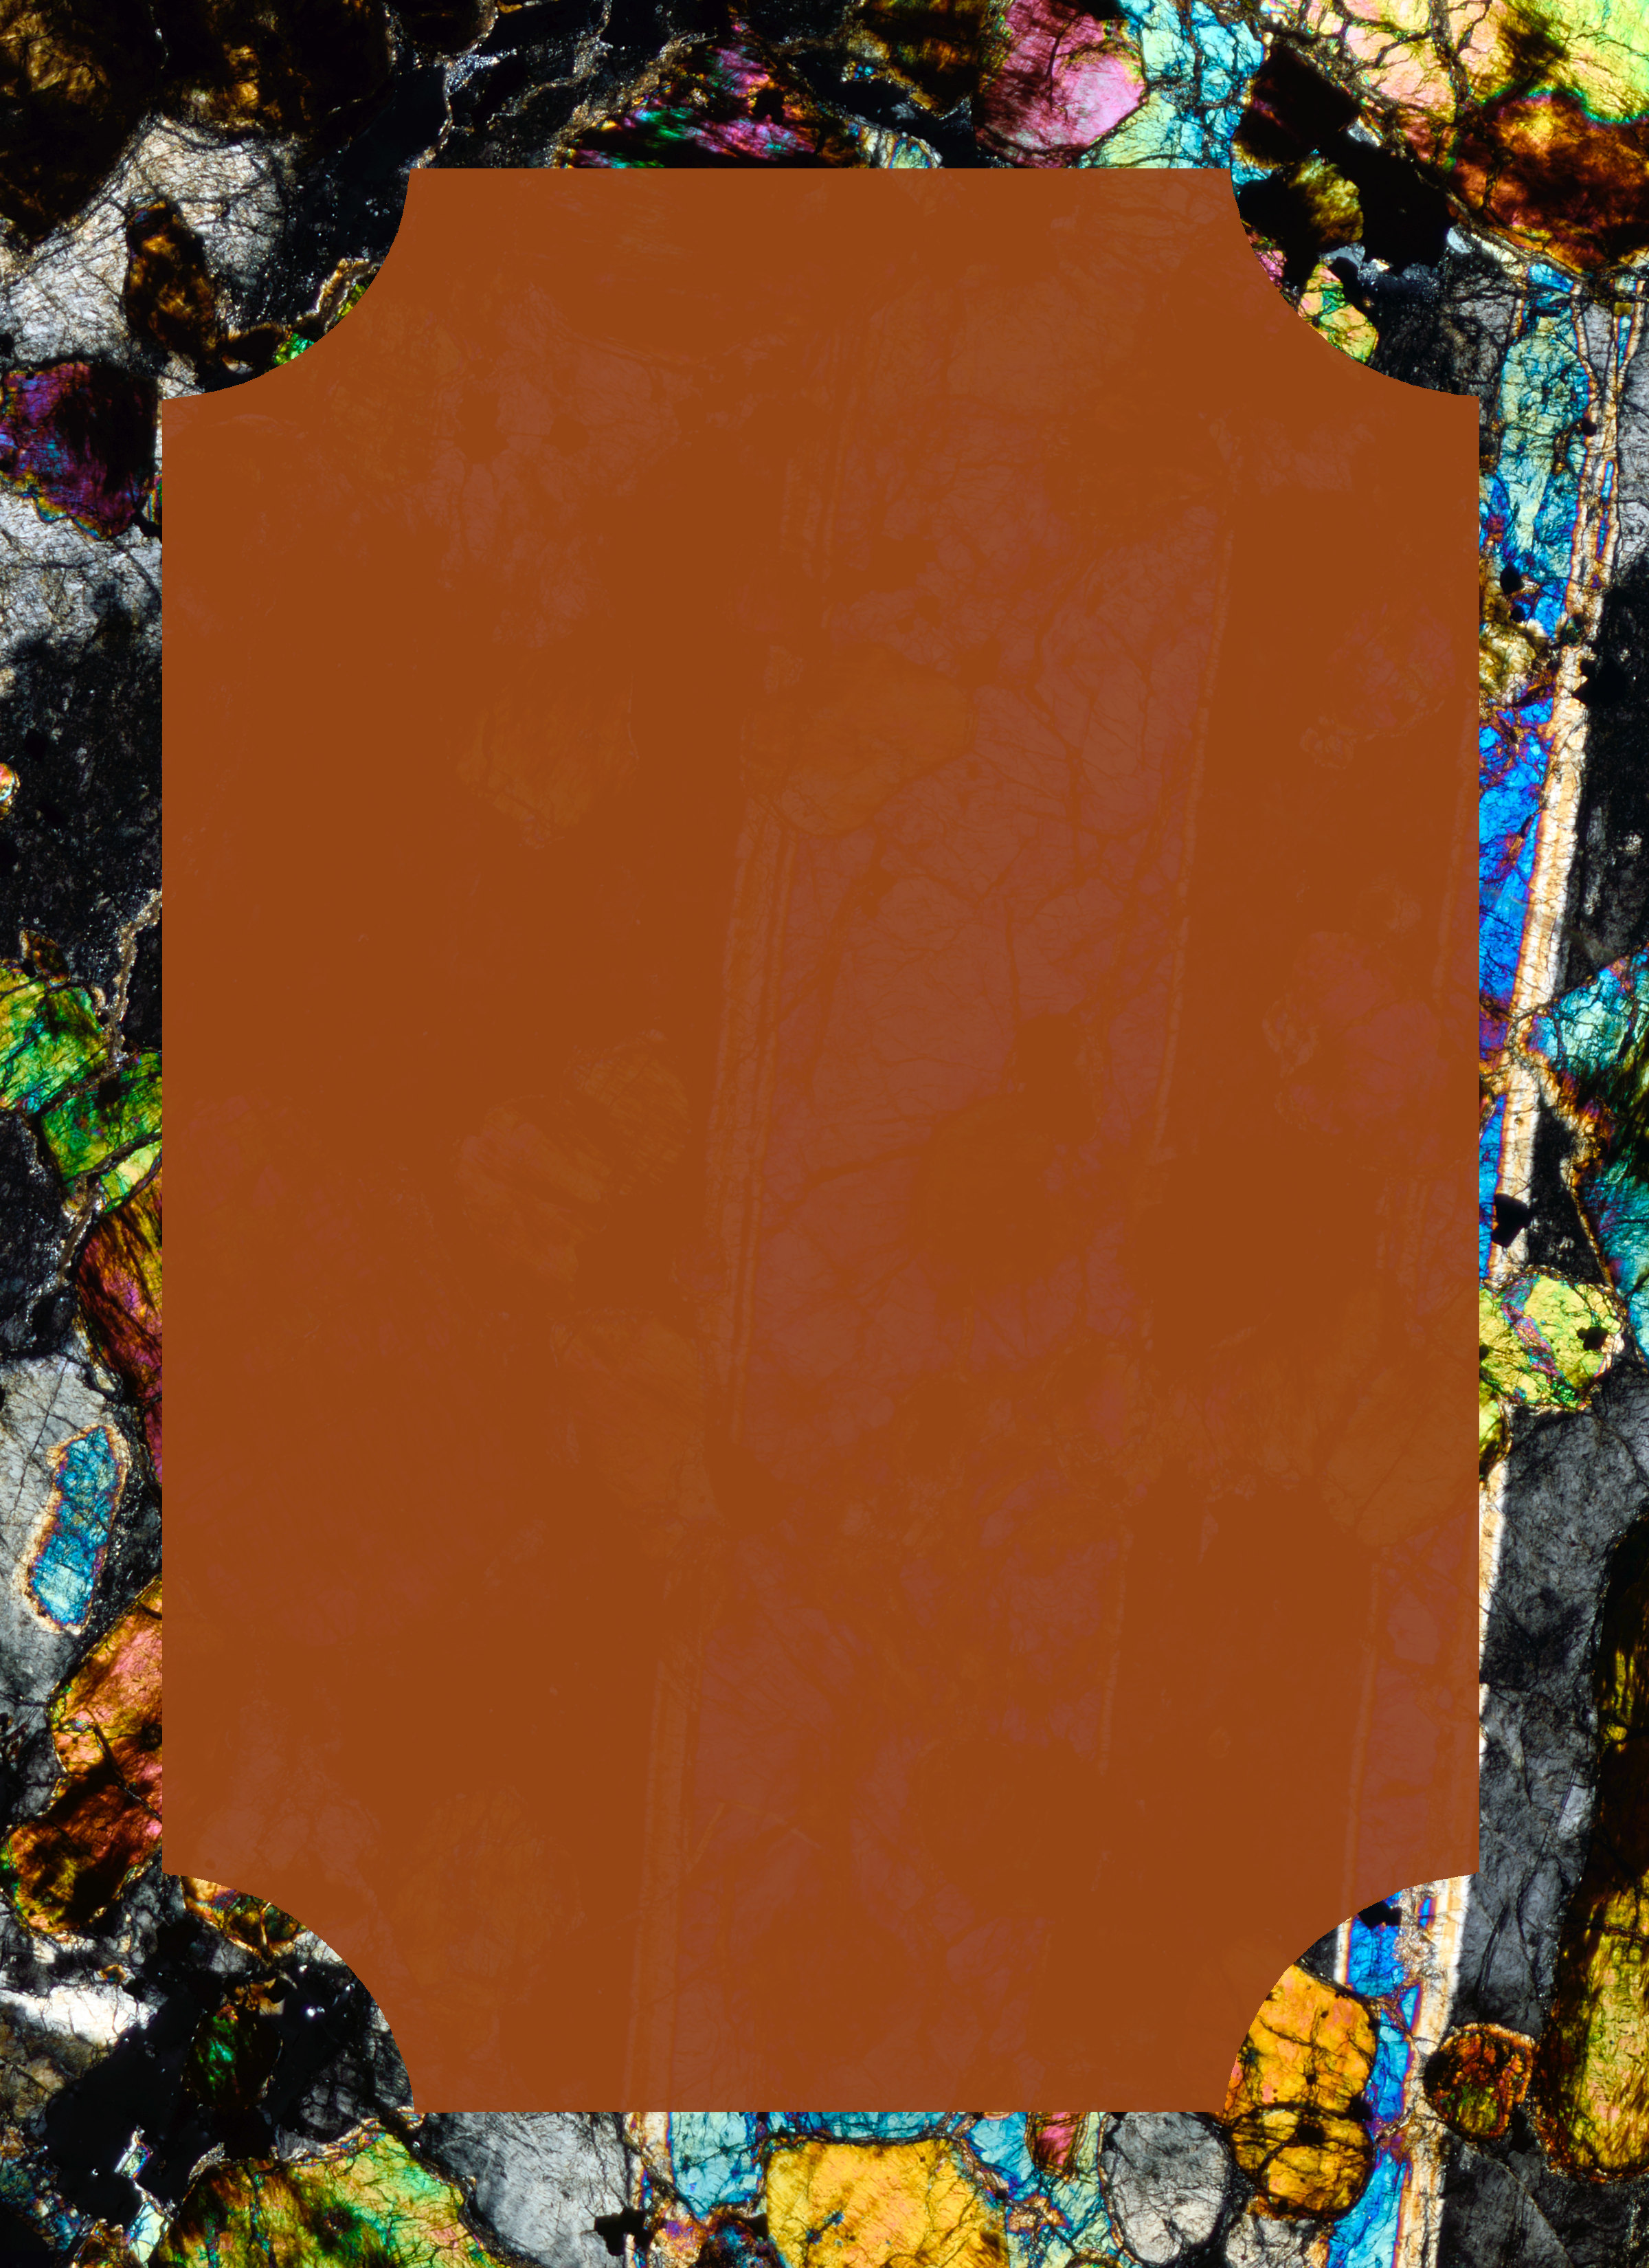
\includegraphics[width=\paperwidth,height=\paperheight]{mars2.jpeg}}
\begin{titlepage} % Suppresses headers and footers on the title page
	\centering % Centre everything on the title page
	%\scshape % Use small caps for all text on the title page

	%------------------------------------------------
	%	Title
	%------------------------------------------------
	
	\rule{\textwidth}{1.6pt}\vspace*{-\baselineskip}\vspace*{2pt} % Thick horizontal rule
	\rule{\textwidth}{0.4pt} % Thin horizontal rule
	
	\vspace{1.5\baselineskip} % Whitespace above the title
	
	{\scshape\LARGE Die Meteoriten in Sammlungen,}
	
	\vspace{1\baselineskip} % Whitespace after the title block

	{\scshape\LARGE ihre Geschichte, Mineralogische}

	\vspace{1\baselineskip} % Whitespace after the title block

	{\scshape\LARGE und Chemische Beschaffenheit.}

	\vspace{1.5\baselineskip} % Whitespace above the title

	\rule{\textwidth}{0.4pt}\vspace*{-\baselineskip}\vspace{3.2pt} % Thin horizontal rule
	\rule{\textwidth}{1.6pt} % Thick horizontal rule
	
	\vspace{1\baselineskip} % Whitespace after the title block
	
	%------------------------------------------------
	%	Subtitle
	%------------------------------------------------
	
	{\scshape von Dr. Otto Buchner.} % Subtitle or further description
	
	\vspace*{1\baselineskip} % Whitespace under the subtitle
	
    % Subtitle or further description
    
	%------------------------------------------------
	%	Editor(s)
	%------------------------------------------------
    \vspace*{\fill}

	\vspace{1\baselineskip}

	{\small\scshape Leipzig, 1863.}
	
	{\small\scshape{Verlag von Wilhelm Engelmann.}}
	
	\vspace{0.5\baselineskip} % Whitespace after the title block

    \scshape Internet Archive Online Edition  % Publication year
	
	{\scshape\small Namensnennung Nicht-kommerziell Weitergabe unter gleichen Bedingungen 4.0 International} % Publisher
\end{titlepage}
\setlength{\parskip}{1mm plus1mm minus1mm}
\clearpage
\large
\tableofcontents
\clearpage
\section*{Vorrede.}
\paragraph{}
Erst von der Zeit an, als Chladni seine bewundernsw"urdig scharfsinnige und geistvolle Theorie der Meteoriten aufgestellt,\footnote{Über den Ursprung der von Pallas gefundenen und anderer ihr "ahnlicher Eisenmassen, und "uber einige damit in Verbindung stehende Naturerscheinungen, von E. F. F. Chladni, Riga 1794. 4º. 63 S.} wurde die Aufmerksamkeit der Gelehrten auf Naturereignisse gelenkt, die vor Chladni und selbst noch geraume Zeit danach f"ur physisch unm"oglich gehalten wurden, weil man sie nicht zu erkl"aren wusste. Der Widerstand, den der Glaube an die M"oglichkeit von Meteoritenf"allen fand und der sich im Institut de France gipfelte, wurde erst durch den Steinfall von L'Aigle und durch Biots Gutachten gebrochen. Von da an stritt man sich nicht mehr um die M"oglichkeit, umso mehr aber um die Erkl"arung dieser Ereignisse. Die fr"uher beobachteten Tatsachen waren zum Teil verdreht und nach hergebrachten Vorurteilen gemodelt worden; man passte sie den theoretischen Ansichten an und was nicht passte, wurde bei Seite gelassen oder willk"urlich ge"andert. Jetzt galt es, die wahren Tatsachen festzustellen. Nur wenige Meteoritenf"alle m"ogen in diesem Jahrhundert in Europa oder sonst einem der Kultur zug"anglichen Teil der Erde beobachtet worden sein, ohne dass die dabei niedergefallenen Massen gesammelt, die Tatsachen vor, w"ahrend und nach dem Ereignis festgestellt wurden. Als eine dieser seltenen Ausnahmen ist der Meteorsteinfall zu Montpreis in Steiermark am 31. Juli 1859 zu betrachten. Es fiel ein zwar nur kleiner Stein in Gegenwart von Augenzeugen, aber die aufgenommenen Bruchst"ucke sind verloren!\footnote{Haidinger Wien. Akad. Ber. 14, 373.} Meistenteils aber wurden gerichtliche und private Urkunden aufgenommen, und die Sammlungen fingen an zu wetteifern in ihrem Reichtum an Meteoriten. Jeder neue Fall, jede neue Lokalit"at war zugleich ein neuer Baustein f"ur die Theorie der Meteoriten. Europa und Amerika lieferten die Baumeister. v. Schreibers, v. Widmannst"atten, Partsch, Berzelius, Haidinger, H"ornes, G. Rose, Rammelsberg, W"ohler, v. Reichenbach, L. Smith, Shepard u. A. waren oder sind noch am t"atigsten. Das wissenschaftliche Material verbreitete sich immer mehr, auch in Privatsammlungen, so dass jetzt keine gr"o"sere Sammlung die eine oder die andere Lokalit"at vermisst. Allerdings konnte es nicht ausbleiben, dass nun auch manche absichtliche oder unabsichtliche Irrt"umer mit unterliefen. Backsteine, Eisensauen, selbst von Ratten angefressene Rhabarberwurzeln wurden als Meteoriten beschrieben, abgebildet und analysiert. Oder "achte Meteoriten wurden unter neuen Namen vorgef"uhrt und so willk"urlich neue Lokalit"aten gebildet. So musste notwendig die neue Abteilung der zweifelhaften und der Pseudo-Meteoriten entstehen. In den letzten Jahren sind manche derselben als unzweifelhaft falsch beseitigt, einige wenige auch als wirklich "acht in die Reihe ihrer Br"uder aufgenommen worden. Den Sachkundigen kann es nicht auffallen, dass immer noch einzelne Lokalit"aten zweifelhaft meteorisch sind. Sie wurden im Folgenden allermeist nicht ber"ucksichtigt, sondern fast nur solche aufgenommen, die unzweifelhaft den Charakter als Meteoriten an sich tragen.

Es ist bemerkenswert, dass die chemischen und oryktognostischen, besonders aber die Strukturverh"altnisse der Meteoriten haupts"achlich in der letzten Zeit einem manchmal bis ins Kleinste gehenden Studium unterworfen wurden. Viele irdische Mineralien sind weniger genau untersucht als die Meteoriten. Allerdings dr"angt sich bei diesen das Material auf wenige hundert Lokalit"aten zusammen; aber trotzdem ist das vergleichende Studium derselben au"serordentlich erschwert; denn einmal ist das Material in vielen Sammlungen zerstreut, ohne dass man wei"s, wo man es suchen kann, dann aber ist die Literatur noch viel zerstreuter, so dass es gro"se Schwierigkeiten macht, alle Quellen zu finden, und manchmal geradezu unm"oglich ist, eine oder die andere derselben nachzuschlagen.

Nur wenige Sammlungen besitzen viele Meteoriten-Lokalit"aten. Diese Himmelssteine sind allermeist zu selten und kostbar, um Handelsgegenstand zu sein; manche sind nur in einer einzigen Sammlung. Da und dort findet sich eine gedruckte Angabe, wo ein gewisser Meteorit aufbewahrt wird. Verzeichnisse von Sammlungen sind nur sp"arlich und meist als fliegende Bl"atter gedruckt, um neue Tauschverbindungen ankn"upfen zu k"onnen. Es war daher meine Aufgabe, m"oglichst viele Kataloge von Sammlungen zu erhalten, um festzustellen, welche Meteoriten aufbewahrt werden und wo sie zu finden sind. Leider war es mir trotz mehrere versandter Zirkulare, trotz meiner Bitte in Poggendorffs Annalen und trotz zahlloser brieflicher Bitten nicht m"oglich, von allen ansehnlicheren Sammlungen Verzeichnisse zu erhalten. Eine Auslassung kann demnach nicht mir zur Last gelegt werden. Immerhin aber antworteten die meisten und gr"o"sten Sammlungen, so dass keine wesentliche L"ucke geblieben ist; manche konnte auch noch durch da und dort zerstreute Literaturangaben ausgef"ullt werden. Es w"are gewiss w"unschenswert, den Ver"anderungen im Bestande der Sammlungen folgen zu k"onnen. Ich werde mir es angelegen sein lassen, von Zeit zu Zeit Nachtr"age zu liefern und bitte daher, mich mit dem n"otigen Material versehen zu wollen.

Es ist dies umso w"unschenswerter, als bei dem raschen Wachsen mancher Sammlungen schon in dem Zeitraum, der f"ur das Zusammenbringen der Kataloge n"otig war, sich Ver"anderungen ergeben haben.

Von den folgenden Sammlungen erhielt ich Meteoritenverzeichnisse; bei der Anzahl der Lokalit"aten wurden die zweifelhaften und unrichtigen nicht mitgez"ahlt, auch nicht die synonymen.
\clearpage
\subsection*{"Offentliche Sammlungen.}
\begin{itemize}
    \item Wien, k. k. Hof-Mineralien-Cabinet (durch Herrn Dr. M. H"ornes). Fallorte 194.

    \item London, britisches Museum (durch Herrn N. S. Maskelyne). Nach der neuesten Angabe von Greg in Philos. Mag. Suppl. Jan. 1863 angewachsen auf Fallorte 190.

    \item Berlin, Universit"at (durch Herrn Professor G. Rose). Fallorte 153. J"ungst wesentlich vermehrt aus der Sammlung von Professor L. Smith in Louisville, N. A.

    \item G"ottingen, Universit"at (durch Herrn Professor W"ohler). Fallorte 125.

    \item Paris, Mus. d'Histoire naturelle (durch freundliche Mitteilung des Herrn Professor Delafosse an Herrn Haidinger [Sept. 1859], der die Benutzung hier gestattete). Fallorte 53.

    \item Paris, Ecole des Mines (durch Vermittlung des Herrn Haidinger, der es durch die G"ute des Herrn v. Sénarmont erhielt). Fallorte 44.

    \item Calcutta, Museum der Asiat. Society of Bengal (durch Herrn Haidinger zusammengestellt). Fallorte 37.

    \item Hudson, Ohio, N.A., Western Reserve College (vermittelt durch die Herren Shepard und Greg). Fallorte 33.

    \item Kopenhagen, Universit"at; fr"uher in den Sammlungen K"onigs Christian 8., des k. naturhistorischen Museums und der Universit"at (durch Herrn Professor Forchhammer), [viele Doubletten]. Fallorte 31.

    \item Stockholm, Reichsmuseum (durch Herrn Professor Nordenski"old). Fallorte 29.

    \item Uppsala, Universit"at (durch Herrn Dr. Thalén). Fallorte 24.

    \item Z"urich, vereinigte Sammlung der Universit"at und des Polytechnikums (durch Herrn Professor Kenngott). Fallorte 23.

    \item Bologna, Universit"at (durch Herrn Professor Bombicci). Fallorte 22.

    \item M"unchen, mineralogische Sammlung des Staats (durch Herrn Professor v. Kobell). Fallorte 20.

    \item Stuttgart, k"onigl. Cabinet (durch Herrn Professor Krauss). Fallorte 20.

    \item Heidelberg, Universit"at (durch Herrn Professor Blum). Fallorte 17.

    \item T"ubingen, Universit"at, ohne die v. Reichenbach'sche Sammlung (im Auftrag des Herrn Professor Quenstedt). Fallorte 17.

    \item Dublin, Trinity College (durch Herrn R. P. Greg in Manchester). Fallorte 16.

    \item Freiberg, mineralogische und geognostische Sammlung der Bergschule (durch Herrn Dr. A. Weisbach). Fallorte 14.

    \item Gotha, herzogl. Naturalien-Cabinet (durch Herrn Dr. A. Hellmann). Fallorte 13.

    \item Edinburgh, Universit"at (durch Vermittlung des Herrn Greg in Manchester). Fallorte 12.

    \item Leipzig, Universit"at (durch Herrn Professor Naumann). Fallorte 10.

    \item Gr"atz, Joanneum (durch Herrn Professor Aichhorn). Fallorte 9.

    \item Kiel, Universit"at (durch Herrn Professor Karsten). Fallorte 9.

    \item Trier, Gesellschaft n"utzlicher Forschungen (durch Herrn Gymnasiallehrer Flesch). Fallorte 9.

    \item Pisa, Universit"at (Professor Meneghini, nach Mitteilung des Herrn Greg in Manchester). Fallorte 7.

    \item Darmstadt, grossh. Naturalien-Cabinet (durch Herrn Ministerialrat Schleiermacher). Fallorte 7.

    \item Clausthal, Bergschule (durch Herrn Dr. R"omer). Fallorte 7.

    \item Prag, b"ohmisches National-Museum (durch Vermittlung des Herrn Dr. H"ornes in Wien). Fallorte 6.

    \item Harlem, Museum der holl"andischen Gesellschaft der Wissenschaften (durch Herrn van Breda). Fallorte 6.

    \item Florenz, naturhistorisches Museum (Sign. Cocci, nach Mitteilung des Herrn Greg in Manchester). Fallorte 6.

    \item Utrecht, Universit"at (durch die k. Akademie der Wissenschaften und deren Sekret"ar Herrn Vrolik in Amsterdam). Fallorte 6.

    \item W"urzburg, Universit"at (durch Herrn Dr. Rumpf). Fallorte 6.

    \item Freiburg, Breisgau, Universit"at (durch Herrn Professor Fischer). Fallorte 6.

    \item Gie"sen, Universit"at (durch Herrn Professor Knop). Fallorte 6.

    \item Bern, Universit"at (durch Vermittlung des Herrn Professor Kenngott in Z"urich). Fallorte 5.

    \item Dorpat, Universit"at (durch Herrn Professor Grewingk). Fallorte 5.

    \item Harlem, Teyler'sche Stiftung (durch die Herren Vrolik in Amsterdam und van Breda). Fallorte 5.

    \item Basel, Universit"at (durch Herrn Professor M"uller). Fallorte 4.

    \item Moskau, Universit"at (durch Herrn Dr. Auerbach). Fallorte 4.

    \item Cassel, h"ohere Gewerbeschule (durch Herrn Dr. Schwaab). Fallorte 4.

    \item Stuttgart, polytechnische Schule (nach Mitteilung des Herrn Professor Krauss). Fallorte 4.

    \item Lemberg, Universit"at (durch Herrn Professor Pebal). Fallorte 4. 3 davon unbestimmt.

    \item Marburg, Universit"at (durch Herrn Professor Dunker). Fallorte 3.

    \item Erlangen, Universit"at (durch Herrn Dr. F. Pfaff). Fallorte 3.

    \item Frankfurt a. M., Senckenbergisches Museum (durch Vermittlung des Herrn Kesselmeyer). Fallorte 2.

    \item Helsingfors, Universit"at (durch Herrn Professor A. E. Arppe). Fallorte 2.

    \item Altenburg, naturforschende Gesellschaft des Osterlandes (durch Herrn Rath Zinkeisen). Fallorte 2.

    \item Krakau, Universit"at (durch Herrn Professor Ritter v. Zepharovich). Fallorte 2.

    \item Leiden, naturhistorisches Museum (durch Vermittlung der k. Akademie der Wissenschaften in Amsterdam, Herrn Vrolik). Fallorte 2.

    \item Mannheim, naturhistorischer Verein (durch Herrn Dr. Hirschbrunn). Fallorte 2.

    \item Gie"sen, Realschule (Dr. Buchner). Fallorte 2.

    \item Kopenhagen, Tierarzneischule (durch Herrn Professor Barfoed). Fallorte 1.

    \item G"orlitz, Realschule (durch Herrn Oberlehrer Fechner). Fallorte 1.

    \item Hamburg, naturhistorisches Museum (nach Vermittlung des Herrn Dr. Zimmermann). Fallorte 1.

    \item Innsbruck, Ferdinandeum (durch Herrn Dr. Lindner). Fallorte 1.

    \item Prag, Universit"at (nach Mitteilung des Herrn Dr. H"ornes in Wien). Fallorte 1.

    \item Rotterdam, Kabinett der batavischen Gesellschaft (durch Vermittlung der k. Akademie der Wissenschaften in Amsterdam, Herrn Vrolik). Fallorte 1.

    \item Washington, Smithsonian Institution (durch Herrn Jos. Henry). Fallorte 1.
\end{itemize}
\clearpage
\subsection*{Privatsammlungen.}
\begin{itemize}
    \item R. P. Greg, Esq. Manchester (1863, Febr. 23). Fallorte 191.

    \item v. Reichenbach, auf Schloss Reisenberg bei Wien. Fallorte 176. Ohne die unter verschiedenen Namen doppelt gez"ahlten; dabei 6 unbekannte (die Sammlung geht sp"ater in den Besitz der Universit"at T"ubingen "uber).

    \item Ch. U. Shepard, Professor am Amherst College New-Haven (die Sammlung ist zur Sicherheit in diesem College aufbewahrt). Fallorte 151. Darunter sehr bedeutende Massen.

    \item Mr. Nevill, Gresham Str. West, London (durch Mitteilung des Herrn Greg). Fallorte 101.

    \item Dr. Auerbach, Professor in Moskau. Fallorte 76.

    \item Dr. K. H. Neumann, k. k. Gubernial- und Commerz-Rath in Prag. Fallorte 61.

    \item Dr. Lawr. Smith, Professor in Louisville (durch g"utige Mitteilung der Herren Haidinger in Wien und Shepard in New-Haven), etwa Fallorte 50. und an gro"sen Massen Fallorte 10. Ist j"ungst wohl gro"senteils in die Berliner Sammlung "ubergegangen.

    \item Duc de Luynes in Dampierre (durch Herrn A. Gory). Fallorte 39. Die Sammlung soll j"ungst an das Musée d'Hist. nat. in Paris "ubergegangen sein.

    \item Dr. Troost in Nashville, jetzt bei Maj. Troost in Mobile, Alabama (nach Mitteilung des Herrn Shepard). Fallorte 9. in sehr gro"sen Exemplaren, au"serdem wohl Fallorte 20. in Bruchst"ucken.

    \item Ferber (Firma Morand \& Co.) in Gera. Fallorte 23.

    \item Dr. K. G. Zimmermann in Hamburg. Fallorte 23.

    \item F"urst Lobkowitz in Bilin (durch Herrn Rubesch). Fallorte 22.

    \item S. K. H. Erzherzog Stephan auf Schaumburg (durch Herrn Siemang\footnote{Ist unterdes gestorben.}). Fallorte 19.

    \item Dr. Buchner in Gie"sen. Fallorte 18.

    \item Dr. med. H. Jordan in Saarbr"ucken (durch Herrn Dr. Weiss). Fallorte 12.

    \item P. A. Kesselmeyer in Frankfurt a. M. Fallorte 12.

    \item Jos. Hieron. Zeidler, Abt des Pr"amonstratenser-Stifts in Prag (durch Herrn Dr. H"ornes in Wien). Fallorte 12.

    \item Dr. Phoebus, Professor in Gie"sen. Fallorte 10.

    \item v. Henikstein in Gr"atz (nach dem Katalog von 1856). Fallorte 9.

    \item Dr. Fischer in Hamburg (durch Herrn Dr. Zimmermann). Fallorte 8.

    \item D. F. Wiser in Z"urich. Fallorte 8.

    \item Dr. v. Baumhauer, Professor in Amsterdam (durch die k. Akademie der Wissenschaften). Fallorte 8.

    \item Dr. R"ossler in Hanau. Fallorte 8.

    \item Kessler, Senator in Frankfurt a. M. (durch Herrn P. A. Kesselmeyer). Fallorte 6.

    \item Max Keller sen. in Freiburg, Breisgau (durch Herrn Professor Fischer). Fallorte 5.

    \item Ulex, Chemiker in Hamburg (durch Herrn Dr. Zimmermann). Fallorte 4.

    \item Dr. Dunker, Professor in Marburg. Fallorte 3.

    \item Dr. van Breda in Harlem. Fallorte 3.

    \item Dr. Osann, Professor in W"urzburg. Fallorte 2.

    \item Meyer, Mineralienh"andler in Hamburg (durch Herrn Dr. Zimmerman). Fallorte 2.
\end{itemize}
\paragraph{}
Die bedeutende Sammlung des Herrn Dr. Krantz in Bonn, deren Verzeichnis mir seiner Zeit ebenfalls vom Besitzer g"utigst mitgeteilt wurde, ging unterdes gr"o"stenteils in andere H"ande "uber und wurde deshalb in der Regel nicht aufgef"uhrt.

Bei dieser Gelegenheit sage ich meinen verbindlichsten Dank allen den hochverehrten G"onnern und F"orderern der Arbeit. Zu ganz besonderem Danke aber bin ich den Herren Haidinger und H"ornes in Wien verpflichtet, welche mich zu dieser Arbeit anregten, fortdauernd mit Literatur und Notizen der verschiedensten Art unterst"utzten, aufmunterten, wenn die Hindernisse scheinbar un"ubersteiglich wurden, und bis zu Ende mit Rat und Tat zur Seite standen. Habe ich eine Arbeit geliefert, die f"ur Forscher und Sammler nicht ganz ohne Nutzen ist, so danke ich es vorzugsweise diesen beiden hochverehrten G"onnern und Freunden.

Trotz meiner Bem"uhungen, keine wichtigere Mitteilung zu vernachl"assigen, w"are es immerhin m"oglich, dass bei der ausgedehnten und "uberall zerstreuten Literatur eine Notiz "ubersehen worden w"are. Dann bitte ich um freundliche Nachsicht und Mitteilung der Auslassung, damit sie an geeignetem Orte nachgetragen werden kann. Es k"onnte mir zum Vorwurf gemacht werden, dass ich v. Reichenbachs ausgedehnte Untersuchungen "uber die Strukturverh"altnisse der Meteoriten, besonders der Eisenmassen, zu sehr vernachl"assigt habe. Doch sind diese Untersuchungen noch zu neu und besonders vom kristallographischen und chemischen Standpunkt aus noch zu wenig best"atigt. Auch G. Rose hat bei seiner neuen Einteilung der Meteoriten der Berliner Sammlung einen anderen Weg betreten.

Bei der "`Literatur"' wurden nur die wichtigsten Quellen vorz"uglich aus den verbreitetsten Zeitschriften angef"uhrt. Partschs klassische Schrift "uber die Meteoriten in Wien (1843) wurde fortw"ahrend zu Grunde gelegt und deshalb nicht regelm"a"sig zitiert. Auch die handschriftlichen Notizen von Partsch, fortgesetzt von H"ornes, wurden mir von Wien mit r"uhmenswerter Bereitwilligkeit und Freundlichkeit zur Benutzung "uberlassen. Wer ausgedehntere Literaturnachweise w"unschen sollte, den erlaube ich mir auf meine beiden Quellenverzeichnisse zur Literatur "uber Meteoriten zu verweisen, die im Band 3 und 4 der Abhandlung gen der Senckenbergischen naturforschenden Gesellschaft in Frankfurt a. M. zu finden sind. Die Theorie der Meteoriten habe ich fr"uher besonders bearbeitet.\footnote{O. Buchner Die Feuermeteore, insbesondere die Meteoriten historisch und naturwissenschaftlich betrachtet. Gie"sen, Ricker, 1859.}

Die Gewichtsangaben wurden auf das franz"osische Grammgewicht reduziert. Eine Verwandlung der L"angenmaasse in das Metermaass lie"s sich nicht durchf"uhren, weil meist selbst nicht mit einiger Gewissheit angenommen werden konnte, welche Meile, welcher Fu"s u. s. w. gemeint war. So blieb da besser die Unbestimmtheit, die sich Jeder ann"ahernd richtig auslegen kann, als dass eine ann"ahernd richtige Übertragung f"ur genau richtig angenommen wird.

Es sind noch viele L"ucken auszuf"ullen. Die von mir nicht verschuldeten sind zugleich ein Fingerzeig f"ur die Forscher. Wo das meiste Material ist, da sollte der Schatz ganz und vollst"andig der Wissenschaft erschlossen werden.

Da noch kein System zur Einteilung der Meteoriten allgemeiner anerkannt ist, so habe ich die chronologische Aufeinanderfolge vorgezogen. Doch habe ich die nat"urlich sich gebenden Gruppen der meteorischen Stein- und Eisenmassen, sowie die vermittelnden Zwischenglieder festgehalten. Nur bei den Steinen schied ich die mit bekannter Fallzeit von denen, deren Fallzeit unbekannt ist. Um jedoch Gelegenheit zu geben, unter den bis jetzt vorgeschlagenen Systemen das einem Jeden am meisten zusagende auszuw"ahlen, lasse ich sie nachstehend folgen.

Gie"sen, Ende M"arz 1863.
\clearpage
\subsection*{System von P. Partsch.}
\begin{center}
Verzeichnis der im k. k. Mineralien-Cabinet zu Wien aufbewahrten Meteoriten.

(Dezember 15, 1862. Von P. Partsch,\footnote{Partsch Die Meteoriten im k. k. Hof-Mineralien-Kabinette zu Wien 1843. Es sind gleichzeitig die gr"o"seren "offentlichen Sammlungen aufgef"uhrt, wo noch Steine und Bruchst"ucke aufbewahrt sind, sowie die Seitenzahl, wo die betreffende Monographie zu finden ist.} fortgesetzt von Dr. M. H"ornes.)
\end{center}
\begin{center}
1. Meteorsteine.
\end{center}
\begin{itemize}
    \item[A.] Anomale (ohne gediegenes und Schwefeleisen, oder im Pulver nur mit dem Mikroskop zu entdecken.)
    \begin{itemize}
        \item[a.] Kohlige Meteoriten.
        \begin{itemize}
            \item Alais. 1806, M"arz 15 (Paris, Berlin, London, Stockholm).
        
            \item Kapland (Cold-Bokkeveld). 1838, Okt. 13 (London, Edinburgh, Petersburg u. A.).
        
            \item Kaba. 1857, Apr. 15 (Debreczin, G"ottingen).
        \end{itemize}
        \item[b.] Schlackenartige Meteoriten.
        \begin{itemize}
            \item Chassigny. 1815, Okt. 3 (Paris, London, Berlin, G"ottingen).

            \item Shalka. 1850, Nov. 30 (Calcutta, London, Berlin).
        \end{itemize}
    \end{itemize}
    \item[B.] Normale (mit Schwefeleisen und z. Th. mit gediegenem Eisen).
    \begin{itemize}
        \item[a.] Ohne metallisches Eisen; die Rinde gl"anzend.
        \begin{itemize}
            \item Juvinas. 1821, Juni 15 (Paris, London, Berlin u. A).

            \item Stannern. 1808, Mai 22 (in den meisten Sammlungen).
        
            \item Konstantinopel. 1805, Juni. 19.
        
            \item Bialistock. 1827, Okt. (Petersburg, Berlin, Dorpat).
        
            \item Luotolaks. 1813, Dez. 13 (Helsingfors, London, Uppsala, Berlin). 
        
            \item Manegaon. 1843, Juli 26 (Calcutta, London).
        
            \item Nobleborough. 1823, Aug. 7.
        
            \item Petersburg. 1855, Aug. 5 (Berlin, London).
        
            \item M"assing. 1803, Dez. 13 (Berlin, Paris, M"unchen).
        
            \item Bishopville. 1843, M"arz 25 (London, Berlin, G"ottingen).
        
            \item Uden. 1840, Juni 12 (Amsterdam, G"ottingen). 
        \end{itemize}
        \item[b.] Mit metallischem Eisen; die Rinde matt (die Steine folgen hier in Gruppen aufeinander, so dass die metall"armsten beginnen und die metallreichsten schlie"sen. Jede Gruppe enth"alt die ihrem Aussehen nach verwandtesten Steine).
        \begin{itemize}
            \item Borgo San Donino. 1808, Apr. 19 (Paris, Berlin, London, G"ottingen).

            \item Okniny. 1833, Dez. 27 (Berlin).
        
            \item Harrison County. 1859, M"arz 28 (London).
        
            \item Siena. 1794, Juni 16 (Berlin, G"ottingen, London, Clausthal).
        
            \item Ensisheim. 1492, Nov. 16 (in den meisten Sammlungen).
        
            \item L'Aigle. 1803, Apr. 26 (in den meisten Sammlungen).
        
            \item Luponnas. 1753, Sept. 7 (Berlin, London).
        
            \item Chandakapoor. 1838, Juni 6 (London, Uppsala, Edinburgh, Kopenhagen).
        
            \item Chantonnay. 1812, Aug. 5 (Berlin, Paris, G"ottingen u. A.).
        
            \item Mainz. ? (G"ottingen, London).
        
            \item Segowlee. 1853, M"arz 6 (Calcutta).
            
            \item Duruma. 1853, (M"unchen).
        
            \item Nulles. 1851, Nov. 5 (Madrid, Barcelona, London).
        
            \item Renazzo. 1824, Jan. 13 (Bologna, Stockholm, Paris, Pisa, Berlin).
        
            \item Richmond. 1828, Juni 4 (London, Berlin, G"ottingen, Paris).
        
            \item Weston. 1807, Dez. 14 (London, Stockholm, Paris, Berlin, G"ottingen).
            
            \item Epinal. 1822, Sept. 13 (Paris, Berlin).
        
            \item Little Piney. 1839, Febr. 13 (London, Berlin).
        
            \item Aussun. 1858, Dez. 9 (Paris, Berlin, London, G"ottingen u. A.).
        
            \item Benares. 1798, Dez. 13 (London, Edinburgh, Paris, Berlin, G"ottingen).
        
            \item Quenggouk. 1857, Dez. 27 (Calcutta, London).
        
            \item Trenzano. 1856, Nov. 12 (London).
        
            \item Utrecht. 1843, Juni 2 (Harlem, Utrecht, G"ottingen).
        
            \item Gouv. Poltava. ? (Petersburg, Berlin).
        
            \item Borkút. 1852, Okt. 13.
        
            \item Krasnoy-Ugol. 1829, Sept. 9 (Petersburg, Berlin).
        
            \item Erxleben. 1812, Apr. 15 (G"ottingen, Berlin, London u. A.).
        
            \item Kleinwenden. 1843, Sept. 16 (Berlin).
        
            \item Gouv. Simbirsk. ? (Petersburg).
        
            \item Iowa. 1847, Febr. 25 (Edinburgh, Berlin, London, G"ottingen).
        
            \item Mauerkirchen. 1768, Nov. 20 (M"unchen, London, Berlin u. A.).
        
            \item Monte Milone. 1846, Mai 8 (Bologna, Pisa, Florenz).
        
            \item Nashville. 1827, Mai 9 (Leiden, Berlin, London, G"ottingen).
        
            \item Kakowa. 1858, Mai 19 (G"ottingen, Berlin).
        
            \item Lucé. 1768, Sept. 13 (Berlin, Z"urich, Freiberg).
        
            \item Lissa. 1808, Sept. 3 (Berlin, London, Paris, Prag, G"ottingen u. A.).
        
            \item Oahu. 1825, Sept. 27 (Dorpat, Berlin, London).
        
            \item Oesel. 1855, Mai 11 (Dorpat, Berlin, G"ottingen, London).
        
            \item Nellore. 1852, Jan. 23 (Madras).
        
            \item Charkow. 1787, Okt. 13 (Charkow, Petersburg, London, G"ottingen, Berlin).
        
            \item Schie. 1848, Dez. 27 (Christiania, London).
        
            \item Zaborzika. 1818, Apr. 10 (Kiew, Berlin, London).
        
            \item Futtehpore. 1822, Nov. 30 (Calcutta, London).
        
            \item Bachmut. 1814, Febr. 3 (Charkow, London, Berlin, Petersburg).
        
            \item Aumières. 1842, Juni 4 (Paris).
        
            \item Pohlitz. 1819, Okt. 13 (Gera, Berlin, London, G"ottingen u. A.).
        
            \item Kuleschowka 1811, M"arz 12/13 (Petersburg, London, Berlin).
        
            \item Girgenti. 1853, Febr. 10 (London).
        
            \item Slobodka. 1818, Aug. 10 (Petersburg, Berlin, Paris).
        
            \item Kikina. 1809.
        
            \item Milena. 1842, Apr. 26 (Agram, Gr"atz, Berlin).
        
            \item Forsyth. 1829, Mai 8 (London, Berlin, Dublin).
        
            \item Wold Cottage. 1795, Dez. 13 (London, G"ottingen, Paris, Berlin).
        
            \item High-Possil. 1804, Apr. 5 (London).
        
            \item Berlanguillas. 1811, Juli 8 (Paris, Berlin, London, G"ottingen).
        
            \item Apt. 1803, Okt. 8 (Paris, Berlin, Gotha).

            \item Vouillé. 1831, Juli 18 (Paris, Berlin).
        
            \item Château-Renard. 1841, Juni 12 (London, Paris, Berlin, G"ottingen).
        
            \item Ohaba. 1857, Okt. 11 (G"ottingen).
        
            \item Salés. 1798, M"arz 8? 12? (London, Paris, Berlin, G"ottingen).
        
            \item Agen. 1814, Sept. 5 (Paris, London, G"ottingen, Berlin).
        
            \item Garz. 1715, Apr. 11 (Berlin, London).
        
            \item Nanjemoy. 1825, Febr. 10 (London, Berlin, G"ottingen, Dublin).
        
            \item New Concord. 1860, Mai 1 (London, Berlin, G"ottingen, Z"urich).
        
            \item S. Denis Westrem. 1855, Juni 7 (G"ottingen).
        
            \item Killeter. 1844, Apr. 29 (London, Dublin).
        
            \item Asco. 1805, Nov. (Berlin).
        
            \item Toulouse. 1812, Apr. 10 (Paris, Berlin, London, Stockholm).
        
            \item Blansko. 1833, Nov. 25 (Berlin, Stockholm).
        
            \item Cereseto. 1840, Juli 17 (Turin, London, Paris, Bologna).
        
            \item Heredia. 1857, Apr. 1 (G"ottingen).
        
            \item Wessely. 1831, Sept. 9 (Br"unn, Berlin).
        
            \item Limerick. 1813, Sept. 10 (Paris, G"ottingen, Berlin).
        
            \item Gr"uneberg. 1841, M"arz 22 (Berlin, Breslau, T"ubingen, London).
        
            \item Tipperary. 1810, Aug. (Dublin, London, Berlin, Kopenhagen).
        
            \item Gouv. Kursk. ? (Petersburg). 
        
            \item Lixna. 1820, Juli 12 (G"ottingen, Berlin, Dorpat, Paris, London).
        
            \item Cabarras County. 1849, Okt. 31 (London, Berlin, G"ottingen).
        
            \item Tabor. 1753, Juli 3 (London, Berlin, Prag, Pesth).
        
            \item Charsonville. 1810, Nov. 23 (Paris, Berlin, Bern, Uppsala).
        
            \item Esnandes. 1837, Aug. (Bordeaux).
        
            \item Doroninsk. 1805, Apr. 10 (Berlin).
        
            \item Mez"o-Madaras. 1852, Sept. 4 (Berlin, London, Kopenhagen, G"ottingen).
        
            \item Assam. 1846. (Calcutta, London).
        
            \item Bremerv"orde. 1855, Mai 13 (G"ottingen, Clausthal, Stockholm, Berlin).
        
            \item Parnallee. 1857, Febr. 28 (London, Berlin, G"ottingen).
        
            \item Dhurmsala. 1860, Juli 14 (Calcutta, London, Berlin, Boston).
        
            \item Mhow. 1827, Febr. 16 (Calcutta, London).
        
            \item Seres. 1818, Juni (G"ottingen, Berlin, London).
        
            \item Sigena. 1773, Nov. 17 (Paris).
        
            \item Kheragur. 1860, M"arz 28 (Calcutta, London).
        
            \item Barbotan. 1790, Juli 24 (London, Paris, Bordeaux, Berlin u. A).
        
            \item Charvallas. 1834, Juni 12 (London).
        
            \item Eichst"adt. 1785, Febr. 19 (M"unchen, Berlin, G"ottingen, London).
        
            \item Gro"s-Divina. 1837, Juli 24 (Pesth).
        
            \item Zebrak. 1824, Okt. 14 (Prag, London).
        
            \item G"utersloh. 1851, Apr. 17 (Berlin, London).
        
            \item Darmstadt. ? (Heidelberg, London).
        
            \item Timochin. 1807, M"arz 13 (Petersburg, Berlin, London, G"ottingen).
        
            \item Macao. 1836, Nov. 11 (Berlin, G"ottingen, Paris, Petersburg).
        
            \item Hainholz. ? (London, Berlin, G"ottingen).
        \end{itemize}
    \end{itemize}
\end{itemize}
\begin{center}
2. Meteoreisen.
\end{center}
\begin{itemize}
    \item[A.] "Astig (mit Olivin in den H"ohlungen).
    \begin{itemize}
        \item Atacama. (London, Paris, G"ottingen, Berlin u. A).

        \item Krasnojarsk. (fast in allen Sammlungen).
    
        \item Oregon.
    
        \item Brahin. (Kiew, Berlin, London, Wien, u. A.).
    
        \item Sachsen (Steinbach, Rittersgr"un). (London, Freiberg, Berlin u. A).
    \end{itemize}
    \item[B.] Derbes Meteoreisen (Einmengungen nur in geringer Menge und nicht von gestaltendem Einfluss auf das Eisen).
    \begin{itemize}
        \item Bitburg. (Berlin, Trier, New-Haven).

        \item Toluca. (G"ottingen, Darmstadt, London, Berlin u. A.).
    
        \item Elbogen. (Prag, Uppsala, Berlin u. A.).

        \item Putnam County. (London, G"ottingen, Berlin, Paris).
    
        \item Oldham County. (London).
    
        \item L"owenfluss. (London, Berlin).
    
        \item Agram (1754, Mai 26) (London, Berlin, G"ottingen u. A.).
    
        \item Lockport. (London, Edinburgh, Dublin).
    
        \item Tazewell. (London, Berlin, Hudson).
    
        \item Robertson County. (London).
    
        \item Lenartó. (Pesth, London, Paris, Berlin u. A).
    
        \item Petropawlowsk. (Petersburg).
    
        \item Schwetz. (Berlin, London, G"ottingen).
    
        \item Madoc. (London, Paris).
    
        \item Nebraska. (London, G"ottingen).
    
        \item Marshall County. (London, Hudson).
    
        \item Denton County. (Austin, G"ottingen).
    
        \item Red River. (New-Haven, London, Berlin u. A).
    
        \item Seneca River. (G"ottingen, London, Berlin).
    
        \item Oaxaca. (Berlin).
    
        \item Oranje River. (London, G"ottingen, Berlin).
    
        \item Rutherford. (London).
    
        \item Durango. (Berlin, London, Paris u. A).
    
        \item Smith County. (London, Berlin, G"ottingen u. A.).
    
        \item Ruffs Mountains. (London, Berlin, Kopenhagen u. A.).
    
        \item Jewell Hill. (London, Hudson).
    
        \item Guilford County. (New-Haven, London, G"ottingen).
    
        \item La Caille. (Paris, Stockholm, Berlin).
    
        \item Burlington. (London, Berlin, G"ottingen, Kopenhagen u. A.).
    
        \item Tula. (London, Berlin).
    
        \item Asheville. (London, Berlin, G"ottingen u. A.).
    
        \item Cocke County. (Berlin, London, G"ottingen u. A).
    
        \item Arva. (London, Berlin, G"ottingen, Uppsala u. A).
    
        \item Tabarz. (G"ottingen).
    
        \item Sarepta. (Berlin, W"urzburg, Stuttgart u. A).
    
        \item Bohumilitz. (Prag, Berlin, G"ottingen u. A).
    
        \item Seel"asgen. (London, Berlin u. A.).
    
        \item Cranbourne. (London, Kopenhagen).
    
        \item Black Mountains. (London, Kopenhagen, G"ottingen).
    
        \item Brazos. (Austin).
    
        \item Union County. (London).
    
        \item Nelson County. (Berlin, London).
    
        \item Bahia. (M"unchen, London, G"ottingen, u. A.).
    
        \item Pittsburg. (G"ottingen).
    
        \item Braunau (1847, Juli 14) (Berlin, Breslau, London u. A.).
    
        \item Tuczon. (London).
    
        \item Concepcion.
    
        \item Saltillo. (Washington).
    
        \item Zacatecas. (London, Berlin, Heidelberg, M"unchen u. A.).
    
        \item Rasgatà. (Paris, Berlin, London, Petersburg, G"ottingen).
    
        \item Scriba. (London, G"ottingen).
    
        \item Tucuman. (London, Kopenhagen, Berlin, Paris, G"ottingen).
    
        \item Salt River. (London, Berlin).
    
        \item Senegal. (Paris, Berlin, London, G"ottingen).
    
        \item Chesterville. (London, Berlin, G"ottingen).
    
        \item Kap der guten Hoffn. (London, G"ottingen, Heidelberg).
    
        \item Green County. (London, G"ottingen, Edinburgh, Berlin).
    
        \item Livingston County. (London).
    
        \item Claiborne. (London, Berlin).
    
        \item Morgan County.
    
        \item Gr"onland. (Kopenhagen u. A.).
    
        \item Madagascar.
    
        \item Hemalga. (London, Edinburgh, Paris).
    \end{itemize}
\end{itemize}
\clearpage
\subsection*{System von G. Rose.}
\begin{center}
Systematisches Verzeichnis der Meteoriten in dem mineralog. Museum der Universit"at zu Berlin.\footnote{Berl. Akad. Ber. 1862, Aug. 7, 14. 1863, Jan. 15.}
\end{center}
\begin{center}
1. Eisenmeteoriten.
\end{center}
\begin{itemize}
    \item[1.] Meteoreisen (nickelhaltiges Eisen, worin Schreibersit (Haidinger), d. i. Phosphornickeleisen (Berzelius) und T"anit (v. Reichenbach), d\. i. eisenhaltiges Nickel (v. Reichenbach d. J.) regelm"a"sig oder unregelm"a"sig eingemengt sind.)
    \begin{itemize}
        \item[a.] Aus einem Individuum bestehend, ohne schalige Zusammensetzung.
        \begin{itemize}
            \item Braunau, Claiborne, Saltillo.
        \end{itemize}
        \item[b.] Aus vielen grobk"ornigen Individuen bestehend.
        \begin{itemize}
            \item Seel"asgen, Zacatecas, Nelson County, Union County, Tucuman.
        \end{itemize}
        \item[c.] Aus einem Individuum bestehend, mit schaliger Zusammensetzung parallel den Fl"achen des Oktaeders (mit Widmannst"atten'schen Figuren).
        \begin{itemize}
            \item Bohumilitz, Arva, Cosbys Creek, Sarepta, Sevier County, Bemdegó, Schwetz, Ruffs Mountain, Seneca River, Toluca, Mistecà, Sierra blanca, Tula, Carthago, Burlington, Marshall County, Oranje River, Red River, Lenartó, Durango, Elbogen, Agram, Asheville, L"owenfluss, Oldham County, Putnam County, Tazewell, Caille, Denton County, Robertson County, Nebraska, Madoc, Black Mountains, Guilford, Lockport, Jewell Hill.
        \end{itemize}
        \item[d.] Aus feink"ornigen Individuen bestehend.
        \begin{itemize}
            \item Tacavita, Rasgatà, Chesterville, Senegal, Kapland, Salt River, Babbs Mill, De Kalb County.
        \end{itemize}
    \end{itemize}
    \item[2.] Pallasit (Meteoreisen mit eingeschlossenen Kristallen von Olivin).
    \begin{itemize}
        \item Krasnojarsk, Brahin, Atacama, Steinbach, Rittersgr"un, Bitburg.
    \end{itemize}
    \item[3.] Mesosiderit (Nickeleisen und Magnetkies einerseits, Olivin und Augit andrerseits in nahezu gleicher Menge).
    \begin{itemize}
        \item Hainholz, Sierra de Chaco.
    \end{itemize}
\end{itemize}
\begin{center}
2. Steinmeteoriten.
\end{center}
\begin{itemize}
    \item[1.] Chondrit (feink"ornige Grundmasse mit eingemengten kleinen Kugeln eines Magnesia-Silikats, mit Kristallen und K"ornern von Olivin, Chromeisenerz und einer unbestimmten schwarzen Substanz, sowie von Nickeleisen und Magnetkies).
    \begin{itemize}
        \item Kleinwenden, Erxleben, Stauropol, Ensisheim, Chantonnay, Tabor, Lucé, Barbotan, Doroninsk, Limerick, Tipperary, Toulouse, Seres, Krasnoy-Ugol, Wessely, Gr"unberg, Cabarras County, Mez"o-Madaras, Renazzo, Luponnas, Eichst"adt, Benares, Nanjemoy, Timochin, Weston, Parma, Lixna, Blansko, Richmond, la Baffe, Poltawa, Macao, G"utersloh, Siena, Bremerv"orde, Parnallee, Aussun, Mauerkirchen, Linn County, Linum, Apt, Bachmut, New-Concord, Honolulu, Kakowa, Charkow, Wold Cottage, Salés, Schellin, L'Aigle, Dhurmsala, Asco, Lissa, Charsonville, Kuleschowka, Berlanguillas, Agen, Zaborzika, Slobodka, Pohlitz, Forsyth, Vouillé, Okniny, Little Piney, Château-Renard, Oesel, Milena, Meno, Futtehpore, Pegu, Trenzano, Ohaba, Charvallas, Mainz.
    \end{itemize}
    \item[2.] Howardit (feink"orniges Gemenge von Olivin mit einem wei"sen Silikat, m"oglicherweise Anorthit, mit einer geringen Menge Chromeisenerz und Nickeleisen).
    \begin{itemize}
        \item Luotolaks, Bialistock, M"assing.
    \end{itemize}
    \item[3.] Chassignit (kleink"orniger eisenreicher Olivin mit eingemengten kleinen K"ornern von Chromeisenerz).
    \begin{itemize}
        \item Chassigny.
    \end{itemize}
    \item[4.] Shalkit (kleink"orniges Gemenge von Olivin, Shepardit [MgO SiO$_{3}$] und Chromeisenerz).
    \begin{itemize}
        \item Shalka.
    \end{itemize}
    \item[5.] Chladnit (Gemenge von Shepardit [MgO SiO$_{3}$] mit einem tonerdehaltigen Silikat, mit geringen Mengen von Nickeleisen, Magnetkies und einigen anderen noch zu bestimmenden Substanzen).
    \begin{itemize}
        \item Bishopville.
    \end{itemize}
    \item[6.] Kohlige Meteoriten.
    \begin{itemize}
        \item Alais, Cold-Bokkeveld, Kaba.
    \end{itemize}
    \item[7.] Eukrit (Gemenge von Anorthit und Augit mit einer geringen Menge Magnetkies und meist viel geringerer Menge Nickeleisen, zuweilen mit gelben Bl"attchen [Juvenas] und Olivin [Petersburg)).
    \begin{itemize}
        \item Juvenas, Stannern, Jonzac, Petersburg.
    \end{itemize}    
\end{itemize}
\clearpage
\subsection*{System von v. Reichenbach.}
\begin{center}
Systematisches Verzeichnis der Meteoriten in der Sammlung des Freiherrn v. Reichenbach zu Wien.\footnote{Nach g"utiger brieflicher Mitteilung d. d. 23. Nov. 1861; erg"anzt nach Poggend. Ann. 107, 166 u. ff. Doch weicht das Verzeichnis daselbst etwas von dem hier gegebenen ab.}
\end{center}
\begin{itemize}
    \item[1. Sippe.] Steine frei von regulinischen Metallen.
    \begin{itemize}
        \item[1.] Gruppe:
        \begin{itemize}
            \item Chassigny, Bishopville. --- Jonzac (Übergangsglied).
        \end{itemize}
        \item[2.] Gruppe:
        \begin{itemize}
            \item Uden, Shalka, Trenzano, Stannern, Juvinas, Konstantinopel, Petersburg.
        \end{itemize}
    \end{itemize}
    \item[2. Sippe.] Steine mit wei"slicher Grundmasse; wenig gediegenes Eisen.
    \begin{itemize}
        \item[1.] Gruppe: Keine dunkeln K"ugelchen, h"ochstens hie und da ein einzelnes zerstreut.
        \begin{itemize}
            \item[a.] Wei"sliche mit leichten Einschl"ussen:
            \begin{itemize}
                \item Nashville, Linn County, Bachmut, Schie, Mauerkirchen, Zaborczika, Futtehpore, Kuleschowka, Milena, Czartorya (?), Wold Cottage, Angers, Forsyth, Girgenti, Ajaquz (?), Pohlitz, Cereseto, Aumières, Charkow, Chandakapoor, Dooralla, Oesel, Garz, Apt, Asco.
            \end{itemize}
            \item[b.] Bl"aulich-wei"se Grundmasse:
            \begin{itemize}
                \item New-Concord, Glasgow, Honolulu, Piemont (?), Château-Renard, Killeter, Lissa, Toulouse, Favars, Berlanguillas, Vouillé.
            \end{itemize}
        \end{itemize}
        \item[2.] Gruppe: Durch eingeschlossene dunkle K"ugelchen grobk"ornig, rau:
        \begin{itemize}
            \item Parma, Eichst"adt, St. Denis Westrem, Zebrak, Little Piney, la Baffe, Nanjemoy, Quenggouk, Benares, Aussun, Lucé, Timochin, Gro"s-Divina, Richmond, Poltava, Borkút.
        \end{itemize}
        \item[3.] Gruppe: dunkle und helle K"ugelchen gemengt:
        \begin{itemize}
            \item Siena, Luotolaks, M"assing, Nobleborough, Bialistock.
        \end{itemize}
    \end{itemize}
    \item[3. Sippe.] Die Grundmasse ist grau, fester als bei den vorigen, nicht zerreiblich, und enth"alt mehr Eisen und weniger Schwefeleisen; das spez. Gew. ist gr"osser.
    \begin{itemize}
        \item[a.] Sigena, Macao, Charsonville.
        \item[b.] Grau und wei"s gefleckt:
        \begin{itemize}
            \item Luponnas, G"utersloh, Weston, Macerata, Okniny, Salés, Mooresfort, Limerick, L'Aigle, Assam.
        \end{itemize}
        \item[c.] Mit wei"slichen Einschl"ussen:
        \begin{itemize}
            \item Cabarras County, Krasnoy-Ugol, Seres, Mez"o-Madaras, Parnallee, Bremerv"orde.
        \end{itemize}
        \item[d.] Dunkelgrau:
        \begin{itemize}
            \item Doroninsk, Cereseto, Agen, Lixna, Chantonnay, Gr"uneberg, Tabor, Blansko, Barbotan, Wessely, Tounkin.
        \end{itemize}
    \end{itemize}
    \item[4. Sippe.] Gr"unliche Grundmasse.
    \begin{itemize}
        \item Ensisheim, Simbirsk, Stawropol, Kleinwenden, Erxleben.
    \end{itemize}
    \item[5. Sippe.] Schwarzbraun und schwarz durch einen starken Kohlegehalt.
    \begin{itemize}
        \item Renazzo, Kaba, Cold-Bokkeveld, Alais.
    \end{itemize}
    \item[6. Sippe.] Die Steine enthalten derbe gr"o"sere braune Anteile.
    \begin{itemize}
        \item Mainz, Segowlee, Charvallas.
    \end{itemize}
    \item[7. Sippe.] Steinige Substanzen sind mit regulinischem Eisen gemengt.
    \begin{itemize}
        \item Mittelglied: Hainholz.
        \item[1.] Gruppe mit reinem Olivin:
        \begin{itemize}
            \item Bitburg, Sachsen, Brahin, Krasnojarsk, Atacama.
        \end{itemize}
        \item[2.] Gruppe Eisen mit Steineinschl"ussen:
        \begin{itemize}
            \item Toluca.
        \end{itemize}
    \end{itemize}
    \item[8. Sippe.] Die kristallinischen Metalle mit Leisten von Nickeleisen; Widmannst"atten'sche Figuren.\footnote{Die hier verzeichneten Eisen teilte v. Reichenbach noch in eine 9. Sippe und diese in 5 Gruppen; doch scheint er diese Einteilung aufgegeben zu haben.}
    \begin{itemize}
        \item[1.] Gruppe:
        \begin{itemize}
            \item Seel"asgen, Cosbys Creek, Bruce, Black Mountains, Bemdeg6, Bohumilitz, Madoc, Burlington, Marshall County, Tula, S. Rosa, Robertson County, Ruffs Mountain, Carthago, Pittsburg, Nebraska, Texas (?), Guilford, Red River, la Caille, Elbogen, Asheville, Agram, Lockport, Oldham County, L"owenfluss, Jewell Hill, Dickson County, Putnam County, Tazewell.
        \end{itemize}
        \item[2.] Gruppe:
        \begin{itemize}
            \item Claiborne (?), Braunau, Nelson County, Cabaja (?), Tucuman, Senegal, Tarapaca.
        \end{itemize}
        \item[3.] Gruppe:
        \begin{itemize}
            \item Cap, Union County, Rasgatà, Livingston County.
        \end{itemize}
        \item[4.] Gruppe:
        \begin{itemize}
            \item Lenartó, Seneca River, Mistecà, Salt River, Chester County, Arva, Davisstra"se, Sarepta, De Kalb, Sevier (?), Zacatecas.
        \end{itemize}
        \item[5.] Gruppe:
        \begin{itemize}
            \item Durango, Schwetz, Oranje River.
        \end{itemize}
    \end{itemize}
\end{itemize}
\clearpage
\subsection*{System von Shepard.}
\begin{center}
System von Shepard.\footnote{Sillim. Amer. Journ. (2) 2, 377. Report on Met. p. 46.}
\end{center}
\begin{center}
1. Classe. Metallische Meteoriten.
\end{center}
\begin{itemize}
    \item[1.] Ordnung. H"ammerbar, gleichartig.
    \begin{itemize}
        \item[1.] Sekt.: Rein (Scriba, Walker County).
        \item[2.] Sekt.: Legiert:
        \begin{itemize}
            \item[a.] Feinkristallinisch (Green County, Texas, Dickson County, Burlington).
            \item[b.] Grobkristallinisch (De Kalb, Asheville, Guilford, Carthago).
        \end{itemize}
    \end{itemize}
    \item[2.] Ordnung. H"ammerbar, ungleichartig.
    \begin{itemize}
        \item[1.] Sekt.: Blasig-olivinisch (Krasnojarsk).
        \item[2.] Sekt.: Blasig-pyritisch (Cambria).
        \item[3.] Sekt.: Pyritisch-graphitisch (Cocke County).
    \end{itemize}
    \item[3.] Ordnung. Spr"ode.
    \begin{itemize}
        \item[1.] Sekt.: Rein (Bedford County, Randolph County).
        \item[2.] Sekt.: Legiert (Otsego County).
    \end{itemize}
\end{itemize}
\begin{center}
2. Classe. Steinmeteoriten.
\end{center}
\begin{itemize}
    \item[1.] Ordnung. Trachytisch.
    \begin{itemize}
        \item[1.] Sekt.: Olivinisch.
        \begin{itemize}
            \item[a.] Grobk"ornig (Weston, Richmond).
            \item[b.] Feink"ornig (Nobleborough, Little Piney).
        \end{itemize}
        \item[2.] Sekt.: Augitisch (Juvinas).
        \item[3.] Sekt.: Chladnitisch (Bishopville).
        \item[4.] Sekt.: Kohlig (Cold-Bokkeveld).
    \end{itemize}
    \item[2.] Ordnung. Trappartig.
    \begin{itemize}
        \item[1.] Sekt.: Gleichartig (Chantonnay).
        \item[2.] Sekt.: Porphyrartig (Renazzo).
    \end{itemize}
    \item[3.] Ordnung. Bimssteinartig (Waterville).\footnote{Nicht meteorisch.}
\end{itemize}
\clearpage
\section{Steinmeteoriten, deren Fallzeit bekannt ist.}
\paragraph{}
Sie sind nach der Fallzeit geordnet.
\subsection{Ensisheim}
\paragraph{}
Ensisheim, Elsass, jetzt Dép. du Haut Rhin, Frankreich.

1492, Nov. 16 (Nov. 7 a. St.), zwischen 11 und 12 Uhr Vormittag.

Ein Stein von 127 K. 270 fiel unter heftigem Get"ose; wahrscheinlich wurde dabei auch eine Feuererscheinung beobachtet. Man sah den Stein in ein Weizenfeld fallen; er wurde bis auf zwei abgeschlagene St"ucke auf Befehl Kaiser Maximilians 1. in der Kirche zu Ensisheim aufgeh"angt, wo er bis zur franz"osischen Revolution blieb; er wurde "ubel zerschlagen, so dass jetzt nur 40-50 K. wieder an der alten Stelle h"angen. Von Sammlungen besitzt das Mus. Hist. nat. in Paris ein St"uck von "uber 9 K. Kleinere Fragmente finden sich in den meisten Sammlungen.

Spezifisches Gewicht:
\begin{table}[!ht]
    \centering
    \bfseries
    \begin{tabular}{l l}
        3,233 & Barthold,\\
        3,5 & v. Schreibers,\\
        3,4884 & Rumler.
    \end{tabular}
\end{table}

Die Rinde fehlt bei den allermeisten Handst"ucken; sie ist br"aunlichschwarz bis schwarz, d"unn, ohne Glanz, etwas rau und in den Vertiefungen glasartig.

Die Grundmasse ist dunkelgrau, feink"ornig, schimmernd, rostbraun gefleckt, stellenweise heller. Bei genauem Betrachten besonders einer geschliffenen Fl"ache unter dem Mikroskop zeigt sich ein unvollkommen breccienartiges Aussehen durch die zahlreichen, vielgestaltigen gr"o"seren und kleineren rundlichen und eckigen dunkelgrau-gr"unen Partien, die in eine hellere Masse eingebettet sind. Die dunkelgraue Substanz ist am wenigsten kristallinisch, sehr feink"ornig bis dicht, wachsgl"anzend, der Bruch uneben bis flach muschelig und splitterig. Die hellgraue Masse ist kristallinisch feink"ornig und mit dunkeln Teilchen gemischt. Unter der Lupe erkennt man noch gelbe bis braune durchscheinende, glasgl"anzende K"ornchen, die an Olivin erinnern, nebenbei auch gro"se schwarze K"ornchen, die an Magnetit erinnern, aber nicht magnetisch sind. Nach Shepard sollen auch Kristalle (0, $\infty$ 0) von Chromeisen darin vorkommen. Nickeleisen ist nicht h"aufig und auf dem Bruch schwer zu erkennen; es ist eingesprengt als sehr kleine, fast silberwei"se K"orner, die z. Th. oxydiert sind. Schwefeleisen ist vorwaltend, teils fein eingesprengt, teils in kleinen Flocken, Nieren und K"ornern, teils als d"unne schuppige Lagen, als Adern. Schwarze gl"anzende Abl"osungsfl"achen, kleine dunkelgraue Facetten, die einer unvollkommen gebildeten Rinde "ahnlichsehen, sind sehr ausgezeichnet und zahlreich, so dass der Stein fast schieferig und leicht spaltbar wird.

Die Analysen sind sehr mangelhaft:
\begin{table}[!ht]
    \centering
    \bfseries
    \begin{tabular}{l l l l l l l}
         & SiO$_{3}$. & MgO. & CaO. & FeO. & Fe. & NiO.\\ \hline
        1. & 42. & 14. & 2. & -,-. & 20. & -,-. \\
        2. & 56. & 12. & 1,4. & 30. & -,-. & 2,4. \\
    \end{tabular}
\end{table}

1. von Barthold, 2. von Fourcroy und Vauquelin. Klaproth wies noch 1,5\% Tonerde und Laugier 0,01\% Chromoxyd nach. Schafh"autl fand eine Verbindung von Schwefeleisen mit Schwefelkupfer, die sich erst in kochender Salzs"aure l"oste.
\footnotesize
\paragraph{}
Viele Chroniken und Urkunden gedenken des Ereignisses (Chladni Feuermet. 205). Barthold Journ. de Phys. 2, 1773, 251. Fourcroy und Vauquelin Gilb. Ann. 13, 295. 18, 280. 319. Laugier ebd. 24, 383. Klaproth ebd. 33, 211. Beitr"age 5, 256. Partsch 32. Shepard Report 8. Schafh"autl M"unchner gel. Anz. 1847, 24, 556.
\subsection{Vago}
\normalsize
\paragraph{}
Dorf Vago unweit Caldiero, Territorium von Verona, Italien.

1668, Juni 19 nach Montanari, oder 21 nach Valisnieri; nach Mitternacht.

Obgleich jedenfalls ein, wahrscheinlich aber zwei sehr gro"se Steine fielen und ausf"uhrliche Mitteilungen dar"uber erhalten sind, auch Bruchst"ucke an die Akademie zu Verona und viele Gelehrte Italiens und Frankreichs geschickt, selbst ein gro"ses St"uck an Ketten in einer Kirche aufgeh"angt wurde, so scheint doch jetzt aus den Sammlungen fast jede Spur verschwunden zu sein. Laugier besa"s 1818 ein kleines St"uckchen; er wies zuerst Chrom darin nach (1\%). Chladni sah diesen Rest und fand ihn Barbotan, Tabor und andern "ahnlich. Wo ist er hingekommen? Catullo beschreibt die schwarze Rinde und vergleicht das Innere mit dem der Steine von Toulouse (1812), nur scheine es mehr metallische Teile zu enthalten. Er sah ein Bruchst"uck in dem fr"uher ber"uhmten Museo Moscardo in Verona, das in den Besitz der Familie Miniscalchi in Verona "uberging; da findet sich vielleicht noch ein Bruchst"uck; die Reste des Museum Moscardo sind jetzt in einer Dachstube des Miniscalchi'schen Hauses wer wei"s in welchem Zustande.
\footnotesize
\paragraph{}
Literatur: Gilb. Ann. 24, 383. Chladni Feuermet. 233. Catullo Geogn. delle prov. Venete 435.
\subsection{Schellin}
\normalsize
\paragraph{}
Schellin (weniger richtig Garz) bei Stargard in Pommern.

1715, April 11, 4 Uhr Nachmittag.

Nach einem Get"ose, das von SO. nach NW. geh"ort wurde, fielen mehre Steine, einer von ca. $7\frac{3}{4}$ K., der zweite kleiner. Der Fall wurde erst 1822 durch Gilbert bekannt. Es haben sich nur sehr wenige kleine Bruchst"ucke erhalten (in Berlin, Wien, London und den Privatsammlungen von v. Reichenbach und Krantz); auch soll ein Gutsbesitzer in Pommern ein Fragment besitzen. Das, welches Prof. Gilbert besa"s, scheint verloren zu sein.

Spezifisches Gewicht: 3,5 Gilbert.

Sie sind au"sen schwarz, "`als wenn sie von Pulver angelaufen, inwendig aber weislicht und glimmend, als ob Metall bei ihnen befindlich und gaben einen schweflichten Geruch von sich."' Auf dem unebenen Bruch zeigt sich ein regelloses Gemenge von vielerlei verschieden abgesonderten K"orpern, die wie eingeknetet zu sein scheinen in eine wei"se, etwas ins Grauliche ziehende dichte erdige Masse. Diese ist weich, selbst zerreiblich; auch einige schwarzgraue K"orner und kleine halbkugelige Vertiefungen, wo offenbar runde K"orner ausgebrochen waren, sind bemerkbar. Durch die ganze Masse sind sehr viele rostfarbene Flecken verbreitet; wo sie angefeilt werden, zeigt sich metallisches Eisen. An mehreren Stellen ragen kleine Eisenmassen "uber die Steinfl"ache hervor. Einzelne nicht verrostete Stellen sind r"otlichgelb, wie Magnetkies; auch findet sich viel schwarzes Eisenoxyd (Magneteisen?).

Der Stein ist noch nicht analysiert worden.
\footnotesize
\paragraph{}
Literatur: Gilbert Annalen 71, 213.
\subsection{Plescowitz und Liboschitz}
\normalsize
\paragraph{}
Plescowitz und Liboschitz, einige Meilen von Reichstadt, Bunzlauer Kreis, B"ohmen.

1723, Juni 22.

Man sah bei heiterem Himmel eine einzelne kleine Wolke und h"orte darin ein starkes Krachen und Knallen, worauf bei Liboschitz 25 und auf anderen herrschaftlich Plescowitz'schen D"orfern unter Funkenspr"uhen 8 gro"se und kleine Steine fielen, die nach Schwefel rochen, auswendig schwarz und inwendig metallisch waren.

Das britische Museum behauptet einen solchen Stein zu besitzen; sonst fehlt er jeder anderen Sammlung, auch Wien. Es ist sehr wahrscheinlich, dass der Stein in London vom Taborfall (1753) herr"uhrt, umso mehr, als er mit den Taborsteinen gro"se "Ahnlichkeit haben soll. Eine genaue Beschreibung desselben ist noch nicht ver"offentlicht; er soll 1844 durch Heuland an das britische Museum gelangt sein.
\footnotesize
\paragraph{}
Literatur: Poggend. Ann. 116, 640.
\subsection{Tabor}
\normalsize
\paragraph{}
Tabor. Hof Krawin bei Strkow, s"udl. von Plan und Tabor.

1753, Juli 3, 8 Uhr Abends.

Nach einer Feuererscheinung erfolgte eine heftige Detonation; dann fielen mehre Steine herab, was von zwei Sch"afern an verschiedenen Stellen beobachtet wurde. Ein ganzer Stein, der erste, der unverletzt in Sammlungen aufbewahrt wurde, ist in Wien und wiegt 2 K. 782,5; au"serdem werden daselbst noch 6 St. aufbewahrt (im Ganzen 4 K. 119,69). Kleinere Bruchst"ucke finden sich in London (164 Gr.), Berlin (77,802 Gr.), Prag (b"ohm. Nat.-Mus.), Pesth (Univ.-Mus.) und den Privatsammlungen des F"ursten Lobkowitz (Bilin, 2 St. 777 Gr.), v. Reichenbach (Wien), v. Henikstein (Gr"atz, 2 St.), Neumann (Prag, 3 St. 74,39 Gr.), Shepard (N. Haven).

Spezifisches Gewicht:
\begin{table}[!ht]
    \centering
    \bfseries
    \begin{tabular}{l l}
        3,234 & Stepling,\\
        4,281 & Bournon,\\
        3,66 & v. Schreibers,\\
        3,6528 & Rumler.
    \end{tabular}
\end{table}

Die Rinde ist matt, schwarz.

In der dunkel-, fast bl"aulich-grauen, rostbraun gefleckten Grundmasse, die dicht und stark zusammenh"angend ist, liegen meist kleine und nicht sehr deutliche K"ugelchen, viel fein und grob eingemengtes, zum Teil auch zu Adern und rundlichen, bis bohnengro"sen Partien vereinigtes Eisen und sehr fein eingesprengter Magnetkies.

Nach Howard werden fast 25\%, vom Magnet ausgezogen. Nach seiner Analyse besteht der erdige Teil aus:
\begin{table}[!ht]
    \centering
    \bfseries
    \begin{tabular}{l l l l l}
        SiO$_{3}$. & MgO. & Fe$_{2}$O$_{3}$. & NiO. & Sa.\\\hline
        45,45. & 17,27. & 42,72. & 2,72. & 108,16
    \end{tabular}
\end{table}

und das h"ammerbare Metall aus:
\begin{table}[!ht]
    \centering
    \bfseries
    \begin{tabular}{l l}
        Fe. & Ni.\\
        89,28. & 10,92.
    \end{tabular}
\end{table}

Meyer hat den Stein nicht selbst analysiert, sondern nur die Prozentberechnung der Analyse Howards bekannt gemacht. Nach Schwefel, der jedenfalls darin enthalten ist, wurde nicht gesucht.
\footnotesize
\paragraph{}
Literatur: Howard Phil. Trans. 1802. Voigt Magaz. 10, 220. Chladni Feuermet. 246.
\subsection{Luponnas}
\normalsize
\paragraph{}
Luponnas (nach dem Dict. des Postes de l'Empire, nicht Liponas oder Laponas) bei Pont-de-Vesle und Bourg-en-Bresse, Dép. de l'Ain, Frankreich.

1753, Sept. 7, 1 Uhr Nachmittag.

Nach heftiger Detonation fielen zwei, vielleicht auch mehr Steine von 10 und fast 6 K. Fragmente finden sich nur in sehr wenigen Sammlungen: Wien (83,673 Gr.), Berlin (1,666 Gr.), London (1,4 Gr.) und in den Privatsammlungen von de Luynes (44 Gr.), v. Reichenbach, Shepard und Greg.

Spezifisches Gewicht: 3,6612 Rumler.

Die Oberfl"ache hat ausgezeichnete Vertiefungen; die Rinde ist matt.

Die dunkelasch- oder bl"aulichgraue Grundmasse wird von schw"arzlichgrauen Partien durchzogen und bekommt dadurch ein fleckiges oder marmoriertes Aussehen; in beiden zeigen sich Rostflecken und ziemlich deutliche, aber mit der Hauptmasse fest verwachsene kugelige Bildungen. Eisen ist fein und mittelfein, Schwefeleisen sehr fein eingesprengt.

Eine Analyse wurde nicht bekannt.
\footnotesize
\paragraph{}
Literatur: Izarn 56 ausf"uhrlicher als Bigot de Morogues 101. Gilb. Ann. 13, 343.
\subsection{Alboreto}
\normalsize
\paragraph{}
Alboreto, unweit Modena, Italien.

1766, Mitte Juli, 5 Uhr Abends.

Unter heftiger Detonation fiel ein sehr gro"ser Stein nieder; ob eine Feuerkugel vorher bemerkt wurde, ist zweifelhaft. Der Stein wurde noch hei"s ausgegraben. Ein St"uck von unbekannter Gr"o"se ist im Mineralienkabinett zu Bologna. Gr"o"sere Sammlungen besitzen nichts davon. Daher sind auch die Beschreibungen sehr mangelhaft und beschr"anken sich auf die Angaben der Zeitgenossen des Falls. Die Oberfl"ache war mit einer dunkeln Rinde "uberzogen, das Innere war sandsteinartig und enthielt zahlreiche Eisenteilchen. Das spezifische Gewicht wird jedenfalls unrichtig als 1,33 angegeben.

Chiodelli analysierte den Stein und fand, dass er aus halbverbranntem Eisen verbunden mit einer scharfen arsenikalischen Substanz bestehe, die beide sich zuf"allig mit fetter und sandiger Erde vermischt h"atten. Diese Analyse ist gar nichts wert.
\footnotesize
\paragraph{}
Literatur: v. Ende Massen und Steine 44. Chladni Feuermet. 250.
\subsection{Lucé}
\normalsize
\paragraph{}
Lucé, Maine, jetzt Dép. de la Sarthe, Frankreich.

1768, Sept. 13, $4\frac{3}{4}$ Uhr Nachmittag.

Ohne dass eine Feuererscheinung wahrgenommen wurde, fiel nach heftiger Detonation aus einer dunkeln Wolke in gekr"ummter Linie ein Stein von fast 4 K. nieder, der so hei"s war, dass man ihn nicht angreifen konnte. Er zerbarst beim Auffallen. Bruchst"ucke sind nur in wenigen Sammlungen: Wien besitzt 3 St. (166,797 Gr.), Berlin (22,657 Gr. aus Chladnis Sammlung, nach Partsch verschieden von den Wiener St"ucken), Z"urich (Universit"at und Polytechnikum 14,5 Gr.), Freiberg (10 Gr.) und die Privatsammlungen von v. Reichenbach, Shepard und Greg. Der gr"o"ste Stein war fr"uher in der Sammlung des Ministers Trudaine in Montigny.

Spezifisches Gewicht:
\begin{table}[!ht]
    \centering
    \bfseries
    \begin{tabular}{l l}
        3,535 & Lavoisier und Cadet,\\
        3,4726 & Rumler.
    \end{tabular}
\end{table}

Die Rinde ist schwarz, matt, rau, an einigen Stellen blasig und gibt am Stahl schwache Funken.

Die Grundmasse ist lichtgrau, unter der Lupe kristallinisch k"ornig; sie besteht aus helleren und dunkleren Teilchen; einzelne dunklere K"ornchen erinnern an undeutliche Kristalloide, zeigen aber keine Spaltungs-, sondern fast splitterige Bruchfl"achen. Sie enth"alt Rostflecken und ist durchs"aet mit undeutlichen kugeligen Absonderungen. In Masse ist Eisen fein und mittelfein, Schwefeleisen sehr fein eingesprengt.

Lavoisier und Cadet, als Kommission der Akademie, analysierten den Stein und fanden:
\begin{table}[!ht]
    \centering
    \bfseries
    \begin{tabular}{l l}
        Schwefel & 8,5\\
        Eisen & 3,6\\
        Verglasbare Erde & 55,5
    \end{tabular}
\end{table}

Die Kommission schloss daraus, dass der Stein weder durch den Donner entstanden, noch vom Himmel gefallen sei; am wahrscheinlichsten schien es ihr, er habe unter dem Rasen gelegen und sei durch einen Blitz oberfl"achlich geschmolzen und herausgeschleudert worden.
\footnotesize
\paragraph{}
Literatur: Das Geschichtliche bei Izarn Lithologie 61, 192, 301 ausf"uhrlicher, als bei Bigot de Morogues 105. Lavoisier und Cadet Mém. Ac. Paris 1769. Journ. de Phys. 1772.
\subsection{Mauerkirchen}
\normalsize
\paragraph{}
Mauerkirchen, damals in Bayern, jetzt im Innviertel, "Osterreich ob der Enns.

1768, Nov. 20, nach 4 Uhr Nachmittag.

Man h"orte ein heftiges Sausen und Brausen, dann fiel ein Stein, der aber erst am folgenden Morgen gefunden wurde; er wog 19 K. und war in zwei St"ucke zerbrochen. Das gr"o"ste, auf vier Seiten mit wohlerhaltener Rinde bedeckte Fragment von 8 K. 802 ist in M"unchen; ferner besitzen Wien (2 St. 581,887 Gr.), London (322 Gr.), Berlin (229,741 Gr.), Kopenhagen (70 Gr.), Kiel (50 Gr.), Gotha (41 Gr.), Harlem (Teylers Mus. 33,8 Gr.), G"ottingen (26 Gr.), T"ubingen (17,5 Gr.), Darmstadt (15 Gr.), Paris (15 Gr.), Stuttgart und Z"urich (klein) und in den Privatsammlungen von Neumann (2 St. 51 Gr.), v. Reichenbach, Shepard, Greg und Kessler.

Spezifisches Gewicht:
\begin{table}[!ht]
    \centering
    \bfseries
    \begin{tabular}{l l}
        3,452 & Imhof,\\
        3,4566 & Rumler.
    \end{tabular}
\end{table}

Die Rinde ist etwas dicker, als bei vielen anderen Meteorsteinen, graulich- oder br"aunlichschwarz, glanzlos, am Stahl Funken gebend.

Die Grundmasse ist hellgrau, fast wei"s, wenig zusammenh"angend, leicht zerreiblich, mit ziemlich vielen, auf den Bruchfl"achen wenig wahrnehmbaren, auf Schnittfl"achen aber leicht erkenntlichen kugeligen Bildungen. Man erkennt kleine plattgedr"uckte, eckige, schwarzgraue, gl"anzende K"ornchen und andere, die wei"s und gelblich, durchscheinend und schimmernd sind. Sehr geschmeidiges und z"ahes Eisen ist in feinen K"ornern und Zacken, viel Schwefeleisen sehr fein, aber auch zuweilen in K"ornern bis zu Hanfkorn- und Bohnengr"o"se eingesprengt.

Die Analyse von Imhof ist unvollkommen.
\begin{table}[!ht]
    \centering
    \bfseries
    \begin{tabular}{l l l l l l}
        Fe. & Ni. & Fe$_{2}$O$_{3}$. & CaO. & SiO$_{3}$. & S u. Verl.\\\hline
        2,33. & 1,2. & 40,24. & 28,75. & 25,4. & 2,08. \\
    \end{tabular}
\end{table}

\footnotesize
Literatur: Imhof Gilb. Ann. 15, 316. 18, 328.
\subsection{Sena}
\normalsize
\paragraph{}
Dorf Sena, Bezirk Sigena, Aragonien, Spanien.

1773, Nov. 17, um Mittag.

Ein Stein von etwa $4\frac{1}{2}$ K. fiel unter den gew"ohnlichen Umst"anden und wurde noch hei"s gefunden. Die Hauptmasse befand sich im k. Naturalienkabinett zu Madrid, wo sie aber jetzt nicht mehr vorhanden sein soll. Au"serdem sind Bruchst"ucke in Paris (Mus. Hist. nat. 58 Gr.), Wien (3,828 Gr.) und in v. Reichenbachs Sammlung.

Spezifisches Gewicht: 3,6382 Rumler.

Der Stein war unregelm"a"sig eif"ormig; auf einer abgeplatteten Basis erhob sich eine dreiseitige stumpfe Pyramide mit abgerundeten Kanten.

Die Rinde ist schwarz und glasig.

Das Innere ist bl"aulich-, fast dunkelgrau, wie Sandstein, es schlie"st wenige eif"ormige, abgerundete K"orner ein, deren gr"o"ste wie Hanfk"orner gro"s sind; zwischen diesen liegen die metallischen und schwefelhaltigen Teile. Das Eisen ist ungleich verteilt, meist fein eingesprengt.

Proust analysierte den Stein und fand:

\begin{table}[!ht]
    \centering
    \bfseries
    \begin{tabular}{l l l l l l}
        FeS. & FeO.\footnote{Schwarzes Eisenoxyd.} & SiO$_{3}$. & MgO. & CaO, MnO. & Sa. \\ \hline
        12. & 5. & 66. & 20. & Spur. & 103. \\
    \end{tabular}
\end{table}

Wird das FeS st"ochiometrisch zerlegt, und aus Prousts Eisenbestimmungen, die zuerst 17, dann 19, dann 22 Th. Eisen gab, welches 3\% Nickel enthalten soll, das Mittel genommen, so ergibt die Analyse:
\begin{table}[!ht]
    \centering
    \bfseries
    \begin{tabular}{l l l l l l l}
        FeO. & SiO$_{3}$. & MgO. & CaO, MnO. & Fe-Ni. & S. & Sa. \\ \hline
        5. & 66. & 20. & Spur. & 7,54.--- & 4,46. & 103. \\
         &  &  &  & 18,753. 0,579. &  &
    \end{tabular}
\end{table}

\footnotesize
Literatur: Proust Journ. de Phys. 60, 185. Gilb. Ann. 24, 261. Chladni Feuermet. 253. Partsch 76.
\subsection{Eichst"adt}
\normalsize
\paragraph{}
Eichst"adt (im Wittmess, einer Waldgegend etwa 2 St. v. Eichst"adt).

1785, Febr. 19, nach 12 Uhr Mittags.

Ein Bauerknecht, durch das Get"ose aufmerksam gemacht, beobachtete den Fall des Steins, der hei"s war und den Schnee schmolz. Er wog fast 3 K. und hatte ungef"ahr 1 Fu"s Durchm.; doch scheinen noch mehre gefallen zu sein. M"unchen besitzt 3 St. (611,25 Gr.). Kleinere St"ucke sind in Z"urich (293 Gr.), Wien (2 St. 127,97 Gr.), G"ottingen (25,87 Gr.), Berlin (15,993 Gr.), London (2,275 Gr.), und bei v. Reichenbach.

Spezifisches Gewicht:
\begin{table}[!ht]
    \centering
    \bfseries
    \begin{tabular}{l l}
        3,700 & v. Schreibers,\\
        3,599 & Rumler.
    \end{tabular}
\end{table}

Die Rinde ist d"unn, rau, matt und schwarz.

Das Innere besteht aus einer dunkelgrauen ziemlich grobk"ornigen Grundmasse mit vielen Rostflecken. Auf dem Bruch ragen zahlreiche kleinkugelige leucitartige Einschl"usse hervor. Als zweiter Gemengteil erscheint eine kleinkristallinische hellgraue Substanz, welche die rundlichen dunkleren K"orner gleichsam verkittet, jedoch nur unter der Lupe die kristallinische Bildung erkennen l"asst. Au"ser diesen beiden sieht man auch gr"unliche Teilchen, von denen einzelne kristallinisch sind und zum Teil deutliche gl"anzende Kristallfl"achen zeigen; ihr Bruch ist glasig-muschelig. Eisen ist mittelfein und reichlich eingesprengt, Magnetkies weniger und sehr fein.

Klaproth analysierte den Stein und fand:
\begin{table}[!ht]
    \centering
    \bfseries
    \begin{tabular}{l l l l l l}
        SiO$_{3}$. & MgO. & Fe$_{2}$O$_{3}$. & Fe. & Ni. & S. u. Verl. \\ \hline
        37,0. & 21,50. & 16,50. & 19. & 1,50. & 4,50. \\
    \end{tabular}
\end{table}

\footnotesize
Literatur: Klaproth Beitr"age 6, 296. Gilb. Ann. 13, 338. Partsch Meteoriten 78.
\subsection{Charkow}
\normalsize
\paragraph{}
Gouvernement Charkow. (Auf einem Felde der Slobode Jigalowka, 10 Werst von dem Dorf Bobrik im Sumschen Kreis. Auch bei Lebedin sollen Steine gefallen sein.)

1787, Okt. 1. a. St. Okt. 13. n. St. 3 Uhr Nachmittag.

Nach einem Get"ose, das unzweifelhaft unrichtig als mehre Stunden dauernd angegeben wird, fielen einige Steine, die noch warm ausgegraben wurden. Die Hauptmasse besitzt die Universit"at Charkow. Kleinere St"ucke sind in Petersburg (Akad. d. Wiss.), London (493,9 Gr.), G"ottingen (44,18 Gr., 2 St.), Berlin (2,499 Gr.), Wien (1,64 Gr.), Freiburg im Breisgrau (3 kl. St"uckchen) und in den Privatsammlungen von v. Reichenbach und Greg.

Spezifisches Gewicht: 3,4902 Rumler.

Die Rinde ist grau- bis braunschwarz, fast glatt, wenig gl"anzend und d"unn.

Die lichtaschgraue Grundmasse enth"alt undeutliche K"orner eingemengt, die etwas ins Gr"unliche ziehen. Eisen ist in geringer Menge und fein, Schwefeleisen sehr fein eingesprengt.

Analysen wurden gemacht von Schnaubert und Giese (I) und von Scheerer (II).
\begin{table}[!ht]
    \centering
    \bfseries
    \begin{tabular}{l l l l l l l l}
         & SiO$_{3}$. & MgO. & Mn$_{2}$O$_{3}$. & MnO. & Fe. & Ni. & S. C. \\ \hline
        1. & 48,00. & 22,05. & 6,00. & -,-. & 21,78. & 1,60. & unbest. \\
        2. & 51,0. & 20,5. & -,-. & 4,20. & 19,8. & 1,5. & 3,0. \\
    \end{tabular}
\end{table}

Lowitz fand noch eine Spur Chrom.
\footnotesize
\paragraph{}
Literatur: Gilb. Ann. 31, 321. Mém. Ac. Pétersb. 6, Hist. 47. Erman Arch. 5, 176.
\subsection{Barbotan}
\normalsize
\paragraph{}
Barbotan (Roquefort, Créon, Juillac, Mezin, Eause, Armagnac, Losse, Agen, St. Sever, La Grange), Dép. des Landes, Dép. Lot et Garonne, Dép. du Gers, ehemals Gascogne (danach und wohl auch nach Bordeaux genannt), Frankreich.

1790, Juli 24, nach 9 Uhr Abends.

Ein h"ochst merkw"urdiger und reicher Meteoritenfall, der das gr"o"ste Aufsehen erregte und von den Gelehrten Frankreichs mit Hohn als grobe T"auschung und unglaubliche L"uge aufgenommen wurde.

Eine gro"se Feuerkugel wurde bei klarem Himmel und hellem Mondschein im s"udwestlichen Frankreich gesehen: sie detonierte heftig und dann fielen viele Steine nieder, meist etwa 1 K. schwer, aber auch bis 15 K. Bruchst"ucke sind in vielen Sammlungen. Wien besitzt 2 St. (zusammen 619,621 Gr.), Gr"atz (576 Gr.), London (481,13 Gr.), Paris (411 Gr., 2 St.), Bordeaux (nach Gilb. Ann. 18, 284 ein 15 Zoll langes St"uck), Berlin (302,212 Gr.), Leipzig (239,74 Gr., 2 St.), Darmstadt (78,35 Gr.), Kopenhagen (45,5 Gr., mehre St.), Z"urich (44,6 Gr.), Gotha (33,45 Gr.), Stockholm (17 Gr.), Gr"atz, Uppsala (10,1 Gr.), G"ottingen (8,82 Gr., 2 St.), Calcutta, Hudson und die Privatsammlungen von de Luynes (57,3 Gr., 2 St.), v. Reichenbach, Shepard, Greg (43 Gr.), Neumann (20,2 Gr., 2 St.), Nevill und von Baumhauer.

Spezifisches Gewicht: 3,6209 Rumler.

Die Rinde ist schw"arzlich, matt, ziemlich dick, runzelig.

Die dunkelgraue, stark rostbraun gefleckte, feste Grundmasse enth"alt sehr wenige kugelige Einschl"usse, stellenweise feine schwarze Adern und meist fein eingesprengtes Eisen, das aber auch in linsen- bis bohnengro"sen K"ornern, sowie in unvollkommenen W"urfeln auftritt. Schwefeleisen ist nur sehr fein eingesprengt, wurde aber von Vauquelin bei der Analyse vernachl"assigt. Er fand:
\begin{table}[!ht]
    \centering
    \bfseries
    \begin{tabular}{l l l l l l}
        SiO$_{3}$. & MgO. & CaO. & Fe$_{2}$O$_{3}$. & NiO. & Sa. \\ \hline
        46. & 15. & 2. & 38. & 2. & 103. \\
    \end{tabular}
\end{table}

\footnotesize
Literatur: Gilb. Ann. 13, 346. 421. 15, 320. 328. 429. 18, 284.
\subsection{Siena}
\normalsize
\paragraph{}
Siena in Toskana, Italien.

1794, Juni 16, nach 7 Uhr Abends.

Unter heftigen Detonationen fielen aus einer kleinen feurigen Wolke viele Steine; dieses W"olkchen kam von Norden her, nach anderen Angaben zog es von Ost nach West, rauchte wie ein Schmelzofen und spr"uhte Funken wie eine Rakete. Es fielen viele, aber kleine Steine, welche sich auf 3 bis 4 ital. Meilen zerstreuten; ein kleiner schlug durch den Hut eines Knaben und versengte ihn. Der gr"o"ste scheint fast $3\frac{1}{2}$ K. gewogen zu haben.

Dieser Steinfall erregte gro"ses Aufsehen; 18 Stunden vorher war ein heftiger Ausbruch des Vesuvs und die Meinung lag nahe, dass die Steine dabei ausgeschleudert worden seien. Doch h"atten sie dann einen Weg von 50 Meilen zur"ucklegen m"ussen. Auch zeigte schon Howard, dass auf dem Vesuv derartige Steine nicht vorkommen. Olbers entwickelte dann seine Mondhypothese, die noch jetzt manche Anh"anger hat, obgleich Olbers selbst davon sp"ater zur"uckkam.

Bruchst"ucke sind in vielen Sammlungen; die meisten besitzt wohl Pisa (3 St. 403 Gr.) und Wien (7 St. 196,87 Gr.), Berlin (52,145 Gr.); in G"ottingen sind 2 ganze Steine mit Rinde (5,09 Gr., 17,5 Gr.), dann finden sich kleinere St"ucke in London (20 Gr.), Clausthal (19,1 Gr.), Bologna, Florenz, Gotha (8,73 Gr.), Z"urich (3,6 Gr.) und in den Privatsammlungen von de Luynes (6,9 Gr.), v. Reichenbach, Greg (215 Gr.), Shepard, Nevill und Buchner.

Spezifisches Gewicht:
\begin{table}[!ht]
    \centering
    \bfseries
    \begin{tabular}{l l}
        3,34-3,40 & Klaproth,\\
        2,986 & Thomson,\\
        3,3-3,4 & v. Schreibers,\\
        3,418 & Bournon,\\
        3,390 & Rumler.
    \end{tabular}
\end{table}
Die Rinde ist zart und fein runzelig-aderig, matt, fast kohlschwarz, zum Teil feinrissig und dadurch wei"s geadert.

Die Grundmasse ist sehr feink"ornig, kristallinisch, hellgrau, zum Teil rostbraun gefleckt, mit vielen zum Teil lichtgr"unlichen oder bernsteingelben, olivinartigen, zum Teil schw"arzlichen, oder dunkelgrauen, wachsgl"anzenden, selten kugeligen, meist eckigen Einschl"ussen, so dass das Ganze breccien- oder porphyrartig aussieht. Magnetkies ist fein, zum Teil auch in K"ornern, das Eisen aber sehr fein in einzelnen zerstreuten K"ornchen und Punkten eingesprengt.

Die Analysen von Howard (1 und 2) und Klaproth (3) haben haupts"achlich historische Wichtigkeit.
\begin{table}[!ht]
    \centering
    \bfseries
    \begin{tabular}{l l l l l l l l l}
         & SiO$_{3}$. & MgO. & FeO. & MnO. & Fe. & Ni. & S. NiO. &  \\ \hline
        1. & 46,66. & 22,66. & 34,66. & -,-. & -,-. & -,-. & -,-. & (Erdige Matrix) \\
        2. & -,-. & -,-. & -,-. & -,-. & 75. & 25. & -,-. & (Metall darin) \\
        3. & 44,0. & 22,5. & 25. & 0,25. & 2,25. & 0,6. & 5,4. &  \\
    \end{tabular}
\end{table}

\footnotesize
Literatur: Gilb. Ann. 6, 46. 13, 296. 312. 18, 285. Pogg. Ann. 24, 222. 105, 441. 111, 355. 371. Chladni Feuermet. 261. Partsch 31.
\subsection{Wold Cottage}
\normalsize
\paragraph{}
Wold Cottage, Yorkshire, England.

1795, Dez. 13, $3\frac{1}{2}$ Uhr Nachmittags.

Dieser Steinfall ist f"ur die Geschichte der Meteoriten von Wichtigkeit, indem die genau beobachteten und von Capitan Topham, bei dessen Wohnung das Ereignis stattfand, zusammengestellten und ver"offentlichten Tatsachen wenigstens in England, wenn auch noch nicht in Frankreich, die Zweifel an die M"oglichkeit eines solchen Ereignisses vernichteten. Bournon und Howard wurden durch diesen Steinfall wesentlich zu ihrer trefflichen Arbeit angeregt, die nachher epochemachend wurde.

Nach heftigen Detonationen, ohne dass gleichzeitig eine Feuerkugel gesehen worden w"are, fiel ein Stein von $25\frac{1}{2}$ K., der von Zeugen des Falles noch hei"s und rauchend ausgegraben wurde. Das gr"o"ste St"uck war lange Eigentum der Familie Sowerby, wurde aber 1838 vom brit. Museum f"ur 2500 fl. gekauft und wiegt jetzt noch 21 K. 581,4 Gr. G"ottingen besitzt 2 St. (134,76 Gr.) und Wien (36,647 Gr.). Au"serdem sind Bruchst"ucke in Paris (7 Gr.), Berlin (2,998 Gr.), Hudson und in den Privatsammlungen von Reichenbach, Shepard, Greg und Nevill.

Spezifisches Gewicht:
\begin{table}[!ht]
    \centering
    \bfseries
    \begin{tabular}{l l}
        3,508 & Bournon,\\
        4,2402 & Rumler.
    \end{tabular}
\end{table}

Die Rinde ist schwarz, matt oder schwach schimmernd.

Die hellgraue, schwach rostbraun gefleckte, ziemlich feste, kaolinartige Grundmasse enth"alt innig verbunden kleine kugelige oder elliptische, manchmal unregelm"a"sig gestaltete K"ornchen und ziemlich viel fein und mittelfein eingesprengtes Eisen, nach Bournon bis zum Gewicht von einigen Grains (zu 0,065 Gr.). Schwefeleisen ist reichlich, aber sehr fein eingesprengt. v. Reichenbach analysierte einen kleinen Einschluss mikroskopisch und bildete ihn ab (Pogg. Ann. 111, 373.).

Bei der chemischen Analyse schied Howard die erdigen Bestandteile (1.) von dem h"ammerbaren Metall (2.) und fand:
\begin{table}[H]
    \centering
    \bfseries
    \begin{tabular}{l l l l l l}
         & SiO$_{3}$. & MgO. & FeO. & NiO. & Sa. \\ \hline
        1. & 50,00. & 24,66. & 32,00. & 1,33. & 107,99. \\
         & Fe. & Ni. &  &  &  \\
        2. & 86,66. & 13,34. &  &  &  \\
    \end{tabular}
\end{table}

\footnotesize
Literatur. Gilb. Ann. 15, 318.
\subsection{Belaja-Zerkwa}
\normalsize
\paragraph{}
Belaja-Zerkwa (Bjelaja-Zerkow nach Eichwald), ehemals Ukraine, Polen, jetzt Gouvernement Kiew, Russland.

1796, Dez. 23. a. St. 1797, Jan. 4. n. St.

In Gegenwart vieler Zeugen fiel unter den gew"ohnlichen Umst"anden ein betr"achtlich gro"ser Stein, der geschmolzen gewesen und erst nach einigen Stunden fest geworden sein soll. Die akademische Sammlung in Kiew (fr"uher in Wilna) besitzt die Hauptmasse. Au"serhalb Russland scheint nur Neumann in Prag ein St"uckchen (0,405 Gr.) zu besitzen.

Über die Beschaffenheit des Steins ist nichts bekannt geworden.

\footnotesize
\paragraph{}
Literatur: Gilb. Ann. 31, 1809, 307.
\subsection{Salés}
\normalsize
\paragraph{}
Salés, bei Villefranche, Dép. du Rhône, Frankreich.

1798, M"arz 8 oder 12, 6 Uhr Abends.

Eine leuchtende Feuerkugel zog von O. nach W. unter furchtbarem Heulen und Prasseln und Funkenspr"uhen. Der Stein, dessen Fall mehre Zeugen in der N"ahe beobachteten, wurde erst am folgenden Morgen ausgegraben; er war nicht mehr hei"s, roch aber schwefelig und hatte an mehreren Stelle Risse: er wog etwa 10 K., doch wurde er zerschlagen. Über die Zeit des Falles finden sich verschiedene Angaben. De Drée, der dem Ereignis am genauesten nachging, aber erst 1802, nennt den 12. M"arz als Falltag. Pictet in Genf sah aber um dieselbe Abendzeit am 8. M"arz eine Feuerkugel von Ost nach West ziehen, so dass dieser Tag vielleicht der richtige ist. --- Sage, der in der Zeit des Unglaubens gleich nach dem Fall ein gro"ses St"uck erhielt, lie"s es in Gestalt einer Vase abdrehen. Existiert wohl noch dieses St"uck gelehrter Barbarei? Das gr"o"ste Bruchst"uck ist in Wien (292 Gr., im Ganzen 334,14 Gr.); kleinere sind in London (191,94 Gr.), Paris (38 Gr.), Berlin (15,993 Gr.), Stuttgart (3 Gr.), G"ottingen (0,92 Gr.) und in den Privatsammlungen von v. Reichenbach, Shepard, Nevill und Greg.

Spezifisches Gewicht:
\begin{table}[!ht]
    \centering
    \bfseries
    \begin{tabular}{l l}
        3,424 & v. Schreibers,\\
        3,4709 & Rumler.
    \end{tabular}
\end{table}

Die Rinde ist schwarz, matt, dick und rau; sie enth"alt einige Eisenk"ornchen und einige graue K"ugelchen; am Stahl gibt sie Funken.

Die Grundmasse ist lichtgrau, etwas ins Dunkle und Braune ziehend, k"ornig und ist von mikroskopisch feinen schwarzen Adern nach allen Richtungen durchwebt, rostbraun gefleckt und schwarz punktiert; von den wenigen kugeligen Einschl"ussen sind sehr wenige schmutzig dunkelgr"un, wenige andere graulichwei"s, sehr zerbrechlich, von dichtem und ebenem Bruch und weicher als die ersteren. Es ist viel Eisen fein und grob manchmal bis zu 3 mm. L"ange eingesprengt, wei"ser und weniger dehnbar als Schmiedeeisen. Schwefeleisen ist teils fein, teils in K"ornchen eingesprengt, teils "uberzieht es die Fl"achen der Risse; es ist bl"attrig, wei"slich und wird vom Magnet angezogen.

Sage analysierte den Stein, ohne an seine meteorische Natur zu glauben. Er fand Nickel, Eisen, Schwefeleisen, Kieselerde und Magnesia. Ohne von Howards Untersuchungen Kenntnis zu haben, unterwarf auch Vauquelin den Stein einer Analyse und fand, nachdem alles Eisen und Schwefeleisen entfernt waren:
\begin{table}[!ht]
    \centering
    \bfseries
    \begin{tabular}{l l l l l l}
        SiO$_{3}$. & Fe$_{2}$O$_{3}$. & MgO. & Ni. & CaO. & Sa. \\ \hline
        46. & 38. & 15. & 2. & 2. & 103. \\
    \end{tabular}
\end{table}

\footnotesize
Literatur: Sage Journ. de Phys. 1803. Avr. p. 314. De Drée Gilb. Ann. 15, 274. 18, 269. Vauquelin ebd. 33, 200.
\subsection{Benares}
\normalsize
\paragraph{}
Bei Benares, besonders bei dem Dorf Krakhut und mehren umliegenden D"orfern. Bengalen, Ostindien.

1798, Dez. 13, 8 Uhr Abends.

Dieser Meteoritenfall ist f"ur die Geschichte der Wissenschaft wesentlich dadurch von Wichtigkeit, dass er die Frage "uber die physische M"oglichkeit solcher Ereignisse wieder in den Vordergrund schob. Aus einer gro"sen Feuerkugel fielen nach heftiger Detonation viele Steine auf einen Umkreis von etwa 2 Meilen. Einer von 1 K. schlug durch das Dach einer H"utte. Viele englische und indische Beamte waren Zeugen des Falles.

Bruchst"ucke sind in mehreren Sammlungen. Das brit. Museum besitzt mehre sch"one St"ucke (zusammen 1 K. 143), Wien 3 St. (das gr"o"ste 561,102 Gr., zusammen 663,918 Gr.), Edinburgh (127,5 Gr.), Dublin, Paris (14 Gr.), Stockholm (8 Gr.), Berlin (5,997 Gr.), G"ottingen (5,41 Gr.) und die Privatsammlungen von v. Reichenbach, Greg, Neumann, Shepard, Auerbach und Nevill.

Spezifisches Gewicht:
\begin{table}[!ht]
    \centering
    \bfseries
    \begin{tabular}{l l}
        3,352 & Bournon,\\
        3,0392 & Kugel aus dem Stein, Rumler,\\
        3,3659 & Stein ohne Rinde, Rumler.
    \end{tabular}
\end{table}

Die Rinde ist dunkelschwarz, stellenweise "ahnlich Firniss, meist matt und d"unn, so dass noch die eingemengten Kugeln zu unterscheiden sind.

Die hellgraue, sehr weiche Grundmasse ist ganz angef"ullt mit teils kugeligen, teils unvollkommen nierenf"ormigen, seltener auch eckigen nadelkopf- bis erbsengro"sen, nur selten gr"o"seren Einschl"ussen von gr"unlicher Farbe, die mit der Masse nur wenig zusammenh"angen, daher aus derselben hervorragen und beim Herausfallen schalige Eindr"ucke hinterlassen. Schwefeleisen ist k"ornig und sehr unregelm"a"sig durch die Masse verteilt. Noch in geringerer Menge tritt das Eisen darin auf.

Die erste Analyse machte Howard, der getrennt untersuchte: 1. die erdige Matrix, 2. die runden Einschl"usse, 3. das h"ammerbare Eisen und 4. das Schwefeleisen. Vauquelin analysierte die Masse ebenfalls 5.
\begin{table}[!ht]
    \centering
    \footnotesize
    \bfseries
    \begin{tabular}{l l l l l l l l l l}
         & SiO$_{3}$. & MgO. & Fe$_{2}$O$_{3}$. & NiO. & Fe. & Ni. & S. & Sa. &  \\ \hline
        1. & 48. & 18. & 34. & 2,5. & -,-. & -,-. & -,-. & 102,5. & Howard, \\
        2. & 50. & 15. & 34. & 2,5. & -,-. & -,-. & -,-. & 101,5. & Howard, \\
        3. & -,-. & -,-. & -,-. & -,-. & 73,91. & 26,09. & -,-. & 100,0. & Howard, \\
        4. & -,-. & -,-. & -,-. & -,-. & 75,00. & 7,14. & 14,28. & 96,42. & Howard, \\
        5. & 48. & 13. & 38. & 3. & -,-. & 3. & X. & 105. & Vauquelin. \\
    \end{tabular}
\end{table}

\footnotesize
Literatur: Gilb. Ann. 13, 291. 15, 423. 41, 453. Chladni Feuermet. 266. v. Schreibers Beitr"age 62. Partsch 43.
\subsection{L'Aigle}
\normalsize
\paragraph{}
L'Aigle (la Vassolerie, Fontenil, la Métonnerie, S. Michel-de Sommaire, St. Nicolas-de Sommaire, Bas Vernet, Mesle, Belangère, la Barne, Bois laville, Corboyer etc.), Normandie, Dép. de l'Orne, Frankreich.

1803, April 26, 1 Uhr Nachmittags.

Dieser Steinfall geh"ort zu den interessantesten und historisch merkw"urdigsten, da er nicht nur der reichste aller bekannten Meteoritenf"alle ist, sondern auch mit ihm alles L"augnen der Tatsache selbst und der Widerstand, den Chladnis Behauptungen im gr"o"sten Teile der wissenschaftlichen Welt fanden, ein Ende hatten. Eine hellleuchtende Feuerkugel war nur in gr"o"serer Entfernung, z. B. in Caen, Falaise, St. Rieux, Pont-Audemer, Verneuil etc. gesehen worden; an den Orten des Steinregens selbst bemerkte man ein kleines, fast unbewegtes, dunkles W"olkchen, aus welchem die Detonationen erschallten, die 30 Meilen in der Runde geh"ort wurden. Dann fielen sehr viele Steine nieder, man nimmt 2000 bis 3000 an, die sich auf einer elliptischen Fl"ache von $2\frac{1}{2}$, Ml. L"ange und 1 Ml. Breite ausstreuten. Fast alle Bewohner von 20 D"orfern dieses Bezirks waren Augenzeugen. In mehreren Orten fielen die Steine hageldicht nieder; alle waren hei"s und verbreiteten starken Schwefelgeruch. Die gro"se Axe der elliptischen Fallfl"ache war von SO. bis NW. gerichtet; die gr"o"sten Steine fielen am SO.-Ende, die kleinsten am entgegengesetzten. Der schwerste wog 8 K. 065.

Hand- und Bruchst"ucke finden sich fast in allen Sammlungen; die gr"o"sten besitzt Wien (4 K. 059,538; der gr"o"ste 1 K. 505), Berlin (2 K. 018,659), London (1 K. 511), Gr"atz (570 Gr.), Z"urich (559 Gr., 5 St.), Freiberg (514 Gr.), Stuttgart (381 Gr., 3 St.), T"ubingen (3 St., der gr"o"ste 240 Gr.), G"ottingen (237,84 Gr., 2 St.), Kopenhagen (184 Gr., 4 St.), Leipzig (173,15 Gr., 3 St.), Paris (Ecole des Mines 154,5 Gr.), M"unchen (125 Gr.), Paris (Mus. Hist. nat. 74 Gr.) und die Privatsammlungen des F"ursten Lobkowitz (2 K. 154, 3 St.), Shepard (987 Gr.), Greg (371 Gr.), Ferber (248 Gr.), van Breda (172,1 Gr., 2 St.), Neumann (117,27 Gr., 2 St.).

Spezifisches Gewicht:
\begin{table}[!ht]
    \centering
    \bfseries
    \begin{tabular}{l l}
        3,584 & Reu"s,\\
        3,626-3,490 & v. Schreibers,\\
        3,279 & Blesson,\\
        3,4791 & ohne Rinde Rumler,\\
        3,3910 & mit Rinde Rumler.
    \end{tabular}
\end{table}

Die Rinde ist braun, matt, klein- und plattnarbig, nicht rau.

Die Grundmasse ist teils hell-, teils dunkelgrau, entweder flockenartig nebeneinander, oder der lichtere Teil ist vom dunkleren in mehr oder weniger dickem aderigen Gewebe durchzogen. Vielfach treten auch rostbraune Flecken auf. Heilere und dunklere, allermeist rundliche K"orner sind der Grundmasse porphyrartig eingemengt, sowie bis bohnengro"se Partien, welche durch Zusammenflie"sen der schwarzen Adern entstanden sind. Schwarze graphitartig aussehende Abl"osungsfl"achen sind nicht selten. Eisen tritt in ziemlicher Menge zum Teil grobk"ornig, Schwefeleisen nur "au"serst feink"ornig auf.

"Altere Analysen existieren von Thénard 1. und Fourcroy und Vauquelin 2.
\begin{table}[!ht]
    \centering
    \bfseries
    \begin{tabular}{l l l l l l l l}
         & SiO$_{3}$. & MgO. & CaO. & FeO. & NiO. & S. & Sa. \\ \hline
        1. & 46. & 10. & -,-. & 45. & 2. & 5. & 108. \\
        2. & 53. & 9. & 1. & 36. & 3. & 2. & 104. \\
    \end{tabular}
\end{table}
\paragraph{}
Laugier wies noch 0,01\%, Chromoxyd nach.
\footnotesize
\paragraph{}
Literatur: Biot Gilb. Ann. 15, 74. Thénard u. A. ebd. 16, 44. 70. Vauquelin u. A. 18, 310. 318. Laugier ebd. 24, 383.
\subsection{Saurette}
\normalsize
\paragraph{}
Saurette bei Apt, Dép. Vaucluse, Frankreich.

1803, Okt. 8, 10 Uhr Vormittag.

Unter heftigem, in weitem Umkreis h"orbarem Krachen fiel ein Stein von etwa 4 K., wovon das gr"o"ste St"uck (1 K.) im Mus. Hist. nat. zu Paris aufbewahrt wird. Kleinere St"ucke sind in Wien (324,845 Gr., 2 St., das gr"o"ste 287,663 Gr.), Berlin (15,993 Gr.), Gotha (5,65 Gr.) und in den Privatsammlungen von v. Reichenbach, de Luynes (9,5 Gr.), Greg und Shepard.

Spezifisches Gewicht: 3,4852 Rumler.

Die Rinde ist schwarz, d"unn, matt und rau.

Die feink"ornige graue Grundmasse ist rostbraun gefleckt und enth"alt einzelne, meist hellere kugelige Einschl"usse. Auf frischem Bruch sind meist die feinen K"ornchen von Eisen und Schwefeleisen kaum zu sehen. Doch ist ersteres zum Teil auch grob eingesprengt.

Laugier fand bei der Analyse:
\begin{table}[!ht]
    \centering
    \footnotesize
    \bfseries
    \begin{tabular}{l l l l l l l l}
        SiO$_{3}$. & MgO. & FeO. & MnO. & NiO. & Cr$_{2}$O$_{3}$. & S. & Verl. u. Wasser (?) \\ \hline
        34. & 14,5. & 38,03. & 0,83. & 0,33. & 0,01. & 9. & 3,31. \\
    \end{tabular}
\end{table}
\footnotesize
\paragraph{}
Literatur: Gilb. Ann. 16, 72. 18, 321.
\subsection{M"assing}
\normalsize
\paragraph{}
M"assing (St. Nicolas) bei Alt"otting, Landger. Eggenfeld in Bayern.

1803, Dez. 13, zwischen 10 und 11 Uhr Vormittag.

Durch heftige Detonationen aufgeschreckt, sah ein Bauer das Niederfallen des Steins, der durch das Dach eines Schuppens schlug und noch ganz hei"s aufgenommen wurde. Er wog etwa 1 K. 600 Gr. Es ist nur noch wenig davon vorhanden. Die gr"o"sten Bruchst"ucke sind in Berlin (23,823 Gr.), Paris (22 Gr.), M"unchen (16,2 Gr.). Ferner sind in Wien (3,25 Gr.), Z"urich (2,8 Gr.) und in den Sammlungen von v. Reichenbach, Neumann (0,25 Gr.) und Greg.

Spezifisches Gewicht:
\begin{table}[!ht]
    \centering
    \bfseries
    \begin{tabular}{l l}
        3,365 & Imhof,\\
        3,3636 & Rumler.
    \end{tabular}
\end{table}

Die Rinde ist d"unn, sehr schwarz und gl"anzend, fast wie gefirnisst.

Die Grundmasse ist graulichwei"s, sehr feink"ornig, ziemlich locker, "ahnlich Bimsteinporphyr und besteht zumeist aus einem wie Feldspat aussehenden lockeren schneewei"sen Mineral von bl"atterig-strahliger Struktur, worin kugelige und eckige Einschl"usse bis Erbsengro"se von unreiner pistaziengr"uner Farbe mit ziemlich vollkommenen schiefwinkligen Teilungsfl"achen, dann kubische schwarze und endlich ganz kleine durchscheinende K"orner und Bl"attchen von gelblicher oder olivengr"uner Farbe zum Teil "uber 1 Linie dick eingemengt sind. Eisen, Schwefeleisen, das unter der Lupe kristallinisch erscheint, und Chromeisen sind fein eingesprengt.

Die Analyse von Imhof ist mangelhaft:
\begin{table}[!ht]
    \centering
    \bfseries
    \begin{tabular}{l l l l l}
        SiO$_{3}$. & MgO. & Fe$_{2}$O$_{3}$. & Fe. & Ni. \\ \hline
        31. & 23,25. & 32,54. & 1,8. & 1,35. \\
    \end{tabular}
\end{table}
\paragraph{}
Im Verlust von 10,06\% sind Schwefel, Chrom etc. enthalten.
\footnotesize
\paragraph{}
Literatur: Gilb. Ann. 18, 330. Schafh"autl M"unchn. Gel. Anz. 1847, 24, 558.
\subsection{High-Possil}
\normalsize
\paragraph{}
Dorf High-Possil bei Glasgow, Schottland.

1804, Apr. 5, Vormittags.

Nach heftigem Get"ose, das von West nach Ost zog und unter den gew"ohnlichen Schallerscheinungen, wobei man eine Rauchwolke, aber kein Feuermeteor beobachtete, fiel ein Stein, der in zwei St"ucke gebrochen, wieder weggeworfen und sp"ater wieder gesucht wurde; er wurde zum Teil gefunden und sind Bruchst"ucke nur in London (91,91 Gr.), Wien (15,313 Gr.) und in Gregs Sammlung (24 Gr.).

Spezifisches Gewicht: 3,5306 Rumler.

Die Rinde ist schwarz und matt, das Innere hellgrau, rostbraun gefleckt, auch schwarz gesprenkelt, mit undeutlichen grauen kugeligen Einschl"ussen. Das Eisen ist fein, meist aber grob eingesprengt, Schwefeleisen aber sehr fein.
\footnotesize
\paragraph{}
Literatur: Gilb. Ann. 24, 369.
\subsection{Doroninsk}
\normalsize
\paragraph{}
Doroninsk, Gouv. Irkutsk, Sibirien.

1805, M"arz 25, nach Eichwald Apr. 10. n. St. 5 Uhr Abends.

Unter heftigem, weithin h"orbarem Get"ose fielen aus einer von Westen kommenden dunkeln Wolke mehre Steine, von welchen zwei gefunden wurden; der erste von fast 3 K. war noch nach $\frac{1}{2}$ Stunde zu hei"s, um ihn zu halten; der zweite wog etwa 1 K. Das gr"o"ste Bruchst"uck scheint Prof. Auerbach in Moskau zu besitzen (179 Gr. mit viel Rinde), Wien hat 61,250 Gr., Berlin 52,312 Gr., Shepard 115 Gr., und Greg 14 Gr.

Spezifisches Gewicht: 3,6154 Rumler.

Die Rinde ist matt und schwarz. Im Anfang soll der Stein au"sen wie mit Ru"s bedeckt gewesen sein, der abgewischt werden konnte, worauf eine dunkelkaffeebraune Oberfl"ache erschien.

Im Innern ist die Masse dunkelaschgrau oder bl"aulich und durch eine Menge Rostflecken fast braun, sehr dicht, mit helleren, undeutlichen kugeligen Einschl"ussen, die mit der Grundmasse fest verwachsen sind und als kleine Flecken erscheinen. Ferner zeigen sich schwarze Abl"osungsfl"achen und undeutliche, sehr feine die Masse durchziehende Adern. Eisen und Magneteisen sind sehr fein eingesprengt.

Die Analyse von Scheerer ist zweifelhaft richtig, gibt auch keinen Aufschluss "uber die Richtigkeit der Angabe, dass der Stein einen salzigen Geschmack gehabt.
\begin{table}[!ht]
    \centering
    \footnotesize
    \bfseries
    \begin{tabular}{l l l l l l l l l l}
        SiO$_{3}$. & MgO. & CaO. & MnO. & Cr203. & Al$_{2}$O$_{3}$. & Fe. & Ni. & S. & Sa. \\ \hline
        40,50. & 9,00. & 6,25. & 1,25. & 2,00. & 3,25. & 18,50. & 10,00. & 8,12. & 98.87. \\
    \end{tabular}
\end{table}
\footnotesize
\paragraph{}
Literatur: Scheerer Mém. Ac. Pétersb. 6. Hist. 46. Stoikowitz Gilb. Ann. 29, 212. 31, 308.
\subsection{Konstantinopel}
\normalsize
\paragraph{}
Konstantinopel, T"urkei.

1805, im Juni.

Am hellen Tage fielen auf dem Fleischplatz mitten in der Stadt mit gro"ser Heftigkeit mehre Steine nieder. Die Griechen, denen man bei diesem Ereignis die Schuld gab, wurden deshalb angefeindet. Aber der Schwefelgeruch und die schwarze Rinde "uberzeugten vom meteorischen Ursprung. Ein Bruchst"uck (7,656 Gr.) befindet sich nur in der Wiener Sammlung und ein kleines St"uckchen bei v. Reichenbach.

Spezifisches Gewicht: 3,17 Rumler.

Die Rinde ist schwarz, schwach gl"anzend, das Innere grau, gleichartig gemengt, stellenweise von d"unnen schwarzen Adern durchzogen. v. Reichenbach analysierte mikroskopisch ein eingeschlossenes Fleckchen.
\footnotesize
\paragraph{}
Literatur: Gilb. Ann. 71, 361. Partsch 26. v. Reichenbach 111, 368. 372.
\subsection{Asco}
\normalsize
\paragraph{}
Asco, Insel Korsika.

1805, November.

Über das Ereignis selbst ist nichts bekannt geworden; der Stein soll in einer Kirche auf Korsika aufbewahrt werden. St"uckchen davon befinden sich nur in den Sammlungen von Wien (18,59 Gr.), Berlin (6,664 Gr.) und v. Reichenbach.

Spezifisches Gewicht: 3,6681 Rumler.

Die Grundmasse ist lichtgrau, mit Rostflecken und kleinen undeutlichen kugeligen Einschl"ussen. Eisen ist fein und mittelfein reichlich eingesprengt. Adern treten sehr fein, schwarz und undeutlich auf.
\footnotesize
\paragraph{}
Literatur: Pogg. Ann. Ergb. 4, 11. 441, Partsch 64.
\subsection{Alais}
\normalsize
\paragraph{}
Alais, eigentlich bei den D"orfern St. Etienne de Lolm und Valence, Dép. du Gard, Frankreich.

1806, M"arz 15, $5\frac{1}{2}$ Uhr Abends.

Unter den gew"ohnlichen Erscheinungen fielen zwei Steine von 4 und 2 K., die beim Aufschlagen in St"ucke zerbrachen. Zeugen beobachteten den Fall und nahmen noch hei"se St"ucke auf. In Sammlungen finden sich nur kleine Fragmente (Paris, Wien, Berlin, London, Stockholm, Z"urich und in den Privatsammlungen von Neumann (Prag), v. Reichenbach, Shepard, Greg, de Luynes und Auerbach.

Spezifisches Gewicht:
\begin{table}[!ht]
    \centering
    \bfseries
    \begin{tabular}{l l}
        1,94 & Biot,\\
        1,7025 & Rumler.
    \end{tabular}
\end{table}

Ganz eigent"umlicher Stein, "ahnlich einer erdigen Kohle. Die Rinde ist br"aunlichschwarz, matt, das Innere ist ebenso gef"arbt, sehr weich und zerreiblich, daher in den Sammlungen als Br"ockchen oder Pulver; beim Reiben nehmen sie Harzglanz an. In Wasser zerf"allt die Masse zu einem graugr"unen Brei mit Tongeruch; an der Luft bedeckt sie sich mit wei"sen Salzausbl"uhungen (nach Berzelius MgOSO$_{3}$ und NiOSO$_{3}$). Auch mit der Lupe lassen sich weder kugelige Einschl"usse, noch Eisenk"ornchen, und nur schwer und selten K"ornchen von gelbem Schwefeleisen unterscheiden. Doch verraten die starken Rostflecken die Gegenwart von Eisen. Am Feuer verbreitet die Masse schwachen Bitumengeruch; vor dem L"otrohr ist sie schwer schmelzbar. Bei abgehaltener Luft erhitzt verliert sie nach Thénard 17\%, dabei CO$_{2}$.

Die Analysen von Thénard, der Kommission des Institut de France (Monge, Fourcroy, Berthollet und Vauquelin) und von Berzelius lassen zweifelhaft, ob der Stein urspr"unglich Wasser enthielt. Entweder wurde der Verlust als Wasser angenommen oder das von Berzelius nachgewiesene Wasser kann auch hygroskopisch aufgenommen worden sein. Am genauesten ist die letzte Analyse. Nach Berzelius l"asst sich die Masse beim Behandeln mit Wasser scheiden in
\begin{enumerate}
    \item 13,28\% mit dem Magnet Ausziehbares; schwarz, glanzlos; vorzugsweise FeOFe$_{2}$O$_{3}$, Spuren von Fe und FeS.
    \item 11,59\% in Wasser L"osliches (MgOSO$_{3}$, CaOSO$_{3}$, NaOSO$_{3}$, KOSO$_{3}$); Spuren von Ni, NH$_{3}$, und einer organischen Substanz. Die meisten dieser Verbindungen bildeten sich vielleicht erst im Laufe der Zeit durch die Einwirkung des oxydierten Schwefeleisens auf die Silikate.
    \item 75,13\%, Hauptmasse. Wird diese der trocknen Destillation unterworfen, so zerf"allt sie in:
    \begin{itemize}
        \item[a.] 88,146\%, schwarzen R"uckstand; brennt sich an der Luft rot; vor dem L"otrohr schwer schmelzbar (s. Analysen unten).
        \item[b.] 0,944\%, graubraunes Sublimat.
        \item[c.] 4,328\%, Kohlens"aure.
        \item[d.] 6,582\%, Wasser. Die entweichende SO$_{2}$ wurde nicht besonders bestimmt.
    \end{itemize}
\end{enumerate}
\paragraph{}
Hier folgen die Analysen von Thénard 1., der Kommission 2. und Berzelius 3.
\begin{table}[!ht]
    \centering
    \bfseries
    \footnotesize
    \begin{tabular}{p{3mm} p{5mm} p{5mm} p{5mm} p{8mm} p{10mm} p{6mm} p{4mm} p{4mm} p{5mm} p{5mm} p{4mm} p{4mm}}
         & SiO$_{3}$. & MgO. & FeO. & Mn. & NiO. & Cr. & C. & S. & Al$_{2}$O$_{3}$. & CaO. & \tablefootnote{\bfseries Zinnoxid und Kupfer.} & \tablefootnote{\bfseries R"uckstand; lie"s sich in ein Silikat von Eisenoxydul und Magnesia zerlegen, dass auch Tonerde, Nickel und Zinn enthielt. Der Verlust bestand zum Teil aus Sauerstoff, der dem Eisen angeh"ort.} \\ \hline
        1. & 21. & 9. & 40. & 2,0. & 2,5. & 1. & 2,5. & 3,5. & -,-. & -,-. & -,-. & -,-. \\
        2. & 30. & 11. & 38. & 2. & 2. (Ni) & 2. & 2,5. & -,-. & -,-. & -,-. & -,-. & -,-. \\
        3. & 31,22. & 22,21. & 29,03. & 0,26. (MnO) & 1,38. & 0,63.\tablefootnote{\bfseries Chromeisen.} & -,-. & -,-. & 2,36. & 0,32. & 0,80. & 8,69. \\
    \end{tabular}
\end{table}
\footnotesize
\paragraph{}
Literatur: Pagès Journ. de Phys. 62, 440. Gilb. Ann. 24, 189. Thénard, Fourcroy etc. ebd. 24, 202. Berzelius Poggend. Ann. 33, 113. Partsch 13.
\subsection{Timochin}
\normalsize
\paragraph{}
Timochin, Kreis Juchnow, Gouv. Smolensk, Russland (Timoschin nach Bl"ode, Timschino nach Eichwald).

1807, M"arz 13. a. St. M"arz 25. n. St. Nachmittags.

Ohne dass eine Feuerkugel bemerkt wurde, fiel unter donnerartigem Get"ose und Krachen ein gro"ser Stein von ca. 70 K. unweit zweier Bauern nieder. Die Hauptmasse von etwa 41 K. besitzt die Akademie der Wissenschaften zu Petersburg. Kleinere Bruchst"ucke sind in vielen Sammlungen: Berlin (437,158 Gr.), Wien (140 Gr., 2 St., der gr"o"ste 83,126 Gr.), Charkow (Bull. Ac. Pétersb. 5, 198), London (56,87 Gr.), G"ottingen (15,4 Gr., 2 St.), Darmstadt (9,3 Gr.) und noch kleinere St"ucke in Z"urich und Kiel; dann in den Privatsammlungen von v. Reichenbach, Erzh. Stephan (55 Gr.), Shepard, Greg und Auerbach.

Spezifisches Gewicht:
\begin{table}[!ht]
    \centering
    \bfseries
    \begin{tabular}{l l}
        3,70 & Klaproth,\\
        3,6046 & Rumler.
    \end{tabular}
\end{table}

Die Rinde ist graulichschwarz, dick, matt und chagrinartig, stellenweise runzelig.

Aus der heller oder dunkler aschgrauen, sehr klein-rostfleckigen, erdigen Grundmasse treten viele dunklere gr"une oder braune kugelige Absonderungen hervor, wodurch das Ganze ein mehr kleinporphyrartiges als mandelsteinartiges Aussehen erh"alt. Eisen tritt reichlich auf in ziemlich starken rauen Zacken, meist aber als K"orner und Punkte, als "astige und zum Teil zusammenh"angende Linien und Adern. Schwefeleisen dagegen ist h"ochst fein in gelben metallgl"anzenden Punkten eingesprengt und selbst auf der Schlifffl"ache nur mikroskopisch wahrnehmbar.

Analysen wurden von Scheerer 1. und Klaproth 2. ausgef"uhrt:
\begin{table}[!ht]
    \centering
    \footnotesize
    \bfseries
    \begin{tabular}{l l l l l l p{25mm} l l}
         & SiO$_{3}$. & MgO. & Fe. & Fe$_{2}$O$_{3}$. & Ni. & (MnO. S. Cr. Verl.) & Al$_{2}$O$_{3}$. & CaO. \\ \hline
        1. & 39. & 20. & 17,75. & 17,5. & 1,25. & 4,5. & -,-. & -,-. \\
        2. & 38. & 14,25. & 17,6. & 25. & 0,4. & 3. & 1. & 0,75. \\
    \end{tabular}
\end{table}
\footnotesize
\paragraph{}
Literatur: Scheerer Gilb. Ann. 29, 213. Klaproth ebd. 33, 210. Bl"ode Bull Ac. Pétersb. 6. 1848. no. 1. Eichwald Erman Arch. 5, 177.
\normalsize
\paragraph{}
Wahrscheinlich ist der Stein von Kikina, Wjasemsker Kreis, Gouv. Smolensk, Russland, der 1809 zu nicht genauer bekannter Zeit gefallen sein soll, ebenfalls von Timochin. Ein Handst"uck lag in der Sammlung des verstorbenen K. W. Rosenberg in Pawlowsk, und in Wien ist noch ein St"uck von 20,781 Gr. Nach Eichwald ist die Masse aschfarben, hat einen braungelben Umfang (okrujnost) mit einer glatten, schwarzen und matten Rinde und enth"alt K"orner von Schwefeleisen und gediegenem Eisen eingesprengt.
\footnotesize
\paragraph{}
Literatur: Eichwald Erman Arch. 5, 177.
\subsection{Weston}
\normalsize
\paragraph{}
Weston, Connecticut, Nordamerika.

1807, Dez. 14, $6\frac{1}{2}$ Uhr Morgens.

Eine von N. kommende, sich schlangenartig bewegende Feuerkugel, welche Funken spr"uhte und einen langen Schweif nachzog, detonierte dreimal und machte jedesmal einen Sprung dabei. Darauf folgten die gew"ohnlichen Explosionserscheinungen und der Steinfall an 6 verschiedenen Orten in der Richtung der Meteorbahn: die ersten fielen mehr nach N., die letzten weiter nach S. Der letzte muss wohl 100 K. gewogen haben, war aber beim Auffallen zerborsten; der gr"o"ste ganze Stein wog fast 16 K., wurde aber zerschlagen. Anfangs waren die Steine weich, wurden aber beim Liegen an der Luft h"arter.

Bruchst"ucke finden sich in vielen Sammlungen. Shepard in New-Haven scheint am meisten davon zu besitzen (708,6 Gr.), London und Wien haben gleichviel (184 Gr.). Kleinere St"ucke sind in Stockholm (55 Gr.), Paris (Ec. des Mines 31,4 Gr., Mus. Hist. nat. 6 Gr.), Kopenhagen (32 Gr.), Berlin (21,158 Gr.), G"ottingen (5,23 Gr.), Dublin, Z"urich (7,5 Gr.), Stuttgart (1,5 Gr.) und in den Privatsammlungen von v. Reichenbach, de Luynes, Greg (125 Gr.), Neumann, Lobkowitz und R"ossler (Hanau).

Spezifisches Gewicht:
\begin{table}[!ht]
    \centering
    \bfseries
    \begin{tabular}{l l}
        3,6 & Silliman,\\
        3,3 & Warden,\\
        3,5854 & Rumler.
    \end{tabular}
\end{table}

Die Rinde ist braunschwarz, matt und rissig, sehr uneben. Innen herrscht die dunkelgraue Farbe vor; durch die Masse zerstreut liegen Flecken von hellerer Farbe, die aber nicht von einem ganz gleichartigen Mineral gebildet und meist mit braunen Rostflecken bes"aet sind. Durch diese Verschiedenheit k"onnen kleine Bruchst"ucke f"ur ganz verschiedenen Lokalit"aten angeh"orig gehalten werden. Sehr reichlich finden sich kleine kugelige Einschl"usse von gelblicher Farbe, die in den dunkleren Partien weit deutlicher auftreten. Shepard h"alt sie f"ur Olivinoid, die unregelm"a"siger gestalteten wie ein Teil der helleren Flecken f"ur Howardit. Schwefeleisen findet sich seltener als gew"ohnlich und ist sehr fein und unregelm"a"sig zerstreut. Nickeleisen tritt sehr reichlich nicht nur in kleinen Punkten, sondern auch in fortlaufenden F"aden und Adern auf, sowie in ovalen Massen manchmal von mehr als 3 Gr. Gewicht. Ja in der Sammlung des Duc de Luynes ist eine Eisenkugel daraus wie ein Kirschkern, 0,04 m. auf 0,025 m., welche 32 Gr. wiegt, wohl die gr"o"ste Eisenkugel, die je in einem Meteorstein gefunden wurde. An einer solchen Eisenkugel fand Shepard auch Glimmer in kleinen br"aunlichgrauen Bl"attchen.

Analysen lieferten Silliman 1. und Warden 2.:
\begin{table}[H]
    \centering
    \footnotesize
    \bfseries
    \begin{tabular}{p{3mm} l l l l l l l l l l}
         & SiO$_{3}$. & Fe$_{2}$O$_{3}$. & MgO. & NiO. & S. & CaO. & Al$_{2}$O$_{3}$. & Cr$_{2}$O$_{3}$. & MnO. & Sa. \\ \hline
        1. & 51,5. & 38. & 13. & 1,5. & 1. & -,-. & -,-. & -,-. & -,-. & 104. \\
        2. & 41. & 30.\tablefootnote{\bfseries (mit Ni.)} & 16. & -,-. & 2,3. & 3. & 1. & 2,3. & 1,3. & 97. \\
    \end{tabular}
\end{table}
\footnotesize
\paragraph{}
Literatur: Gilb. Ann. 29, 353. 42, 210. Sill. Am. Journ. (2) 6, 410.
\subsection{Mooradabad}
\normalsize
\paragraph{}
Mooradabad, Indien.

1808.

Über das Ereignis des Steinfalls ist nichts Genaueres bekannt geworden. Calcutta besitzt 3 St"ucke (70,87 Gr.). In Europa scheint nur London ein Bruchst"uck zu besitzen (17,39 Gr.).

Spezifisches Gewicht: 3,5.

Die Masse ist ziemlich zerreiblich und enth"alt Nickel und Chrom. Der Stein scheint mit der h"aufigsten Art der Meteoriten "ubereinzustimmen.
\footnotesize
\paragraph{}
Literatur: Poggend. Ann. 24, 223.
\subsection{Borgo San Donino}
\normalsize
\paragraph{}
Borgo San Donino, Casignano, bei Parma, Italien.

1808, Apr. 19, zwischen 12 und 1 Uhr Mittags.

Eine Feuererscheinung wurde nicht deutlich wahrgenommen; die Detonation war sehr heftig und ein Stein wurde sofort noch ganz hei"s aufgefunden. Doch fielen viele Steine auf eine Fl"ache von etwa 9 Kilometer Umfang. Der gr"o"ste war oder ist noch in der Sammlung des verstorbenen Grafen Linati in Parma; au"serdem besitzen Bruchst"ucke die Sammlungen in Paris (428 Gr.), Wien (80,391 Gr., 2 St.), Berlin (15,327 Gr.), London (10,465 Gr.), G"ottingen (0,65 Gr.) und die Privatsammlungen von v. Reichenbach, Shepard, de Luynes (2,6 Gr.), Greg (2 Gr.), Neumann (1,7 Gr.).

Spezifisches Gewicht:
\begin{table}[!ht]
    \centering
    \bfseries
    \begin{tabular}{l l}
        3,39-3,46 & Guidotti,\\
        3,399 & Rumler.
    \end{tabular}
\end{table}

Die Rinde ist braunschwarz, d"unn, halb glasartig, fast matt.

In der lichtgrauen Grundmasse liegen viele kleine kugelige und eckige Einschl"usse, wodurch der Stein ein breccienartiges Aussehen erh"alt. Eisen ist fein eingesprengt; Schwefeleisen herrscht vor und tritt auch in gr"o"seren Partien auf.

Nach der Analyse von Guidotti besteht der Stein aus
\begin{table}[!ht]
    \centering
    \bfseries
    \begin{tabular}{l l l l l l l}
        SiO$_{3}$. & MgO. & FeO. & MnO. & NiO. & Cr$_{2}$O$_{3}$. & S. \\ \hline
        50,0. & 19,0. & 28,0. & 1,5. & 2,5. & 1,0. & 4. \\
    \end{tabular}
\end{table}
\paragraph{}
Das Schwefeleisen fand er wenig nickelhaltig. Vauquelin wies in der Steinmasse 0,15\%, Tonerde nach.
\footnotesize
\paragraph{}
Literatur: Gilb. Ann. 29, 210. 33, 198.
\subsection{Stannern}
\normalsize
\paragraph{}
Stannern (Langenpiernitz), Iglauer Kreis, M"ahren.

1808, Mai 22, gegen 6 Uhr Morgens.

Nicht nur die Steine sind h"ochst merkw"urdig, sondern auch der Fall selbst vortrefflich beobachtet, die Tatsachen durch gerichtliche und wissenschaftliche Untersuchungen festgestellt und die Steine in reichlicher Menge sorgf"altig gesammelt; von keinem Ereignis dieser Art sind so viele Steine in derselben Sammlung, so dass ein genaues Studium, ein Vergleichen und eine folgerichtige Zusammenstellung derselben m"oglich ist, wie gerade hier.

Bei heiterem Himmel und pl"otzlich eingetretenem Nebel, der 4 Stunden w"ahrte, h"orte man mehre Detonationen und darauffolgendes Get"ose; die Luftersch"utterung dabei wurde 5-8 Meil. im Umkreis versp"urt. In 4-5 Meil. Entfernung wurde auch eine Feuerkugel mit Schweif von NO. nach SW. gehend gesehen. Es fielen in Gegenwart vieler Augenzeugen viele Steine nieder, nach v. Schreibers etwa 100, nach Partsch 200-300. Schon am sechsten Tage nach dem Fall wurden v. Schreibers und v. Widmannst"atten von Wien aus in die Gegend geschickt, um die Tatsachen festzustellen, was durch die genauesten privaten und gerichtlichen Untersuchungen und Verh"ore, durch 20 Protokolle und "uber 100 private Aussagen vollkommen gelang. 61 Steine konnten nach Wien zur"uckgebracht werden. An ihnen erkannte v. Schreibers Zuerst die vorherrschend pyramidale Gestalt, die unterdessen an so vielen anderen Meteoriten best"atigt worden ist. Die Steine fielen auf eine elliptische Fl"ache, in deren Mittelpunkt der Marktflecken Stannern liegt, und deren gr"o"ste L"ange etwa 7000, die gr"o"ste Breite 2600 Klafter betr"agt. Doch verbreiteten sich hier die Steine nicht gleichm"a"sig, sondern in drei Hauptgruppen entsprechend den drei Hauptdetonationen, die gleich gewaltigen Donnerschl"agen nach manchen Richtungen auf 10 bis 14 Meil. geh"ort wurden. Die erste Fallgruppe liegt am n"ordlichen Ende der ganzen Fl"ache; es wurden 4 Steine gefunden, deren gr"o"ster "uber 8 K. wog; ihr Gesamtgewicht betr"agt 15 K. Zur mittleren Gruppe geh"orten 36 Steine von zusammen fast 31 K.; es waren meist kleinere, der gr"o"ste $2\frac{1}{2}$ K., im Durchschnitt 1-$1\frac{1}{2}$ K. Zur s"udlichsten Gruppe geh"orten 26 Steine im Gesamtgewicht von nur etwas "uber 6 K., also durchweg kleine und sehr kleine Steine, der gr"o"ste etwas "uber 1 K., der kleinste ca. 60 Gr., doch sind ohne Zweifel noch kleinere gefallen, aber der Fallorte nicht genauer bezeichnet worden. In der Wiener Sammlung wiegt der kleinste der Stannern-Steine nur 3,5 Gr. H"atte der Krieg von 1809 den Untersuchungen kein Ende gemacht, so w"aren voraussichtlich --- es wurde das Feld nur zweimal durchsucht --- noch weitere Steine gefunden worden.

Ganze Steine oder Bruchst"ucke sind fast in allen Sammlungen: Die meisten und gr"o"sten in Wien (15 K. 531,031, 35 St., der gr"o"ste 6 K. 384,257), kleinere in Berlin (3 K. 460,649), London (1 K. 079), Innsbruck (Ferdinandeum 600 Gr.), Petersburg (Akademie der Wissensch. 541,7 Gr.), Paris (Mus. Hist. nat. 538 Gr.), Harlem (Teylers Mus. 426,4 Gr.), M"unchen (420 Gr.), G"ottingen (366,72 Gr.), Gr"atz (337 Gr.), Gotha (335 Gr.), Kopenhagen (310 Gr.) und noch kleinere in Breslau (schles. Gesellsch.), Bologna, Calcutta, Freiberg, Gr"atz (loanneum), Heidelberg, Hudson (Res. Coll.), Leipzig, Lemberg, Mannheim (nat.-hist. Verein), Marburg, Sct. Gallen (st"adt. Min.-Cab.), Stockholm, Stuttgart (k. Mus. und polyt. Schule), Trier, T"ubingen, Uppsala, W"urzburg und Z"urich. Auch in vielen Privatsammlungen findet sich diese Lokalit"at, so namentlich bei v. Reichenbach, Erzh. Stephan (617 Gr.), Neumann (393,88 Gr.), Ferber (295,6 Gr.), Greg (275 Gr.), Shepard (222 Gr.), Lobkowitz (215 Gr.) und kleinere bei Auerbach (33 Gr.), v. Baumhauer, Fischer, Jordan, Kessler, de Luynes, Nauck, v. Henikstein, Nevill.

Spezifisches Gewicht:
\begin{table}[!ht]
    \centering
    \bfseries
    \begin{tabular}{l l}
        2,9-3,2 & v. Schreibers,\\
        3,19 & Vauquelin,\\
        2,95-3,16 & Chladni,\\
        3,1527 & ohne Rinde Rumler,\\
        3,1529 & mit wenig Rinde Rumler,\\
        3,0777 & mit viel Rinde Rumler.
    \end{tabular}
\end{table}

v. Schreibers hat ausf"uhrlich die Rinde in allen ihren Verschiedenheiten und mancherlei Eigenschaften und Abweichungen sehr ausf"uhrlich beschrieben. Schon er bemerkt, dass man aus der Richtung der Streifungen auf derselben und ihrem merkw"urdigen Überflie"sen "uber die Kanten auf die Richtung schlie"sen kann, die der Stein w"ahrend des Falles hatte. Noch ausf"uhrlicher hat Haidinger diesen Punkt behandelt und unter andern auch Stannernsteine als Belegst"ucke gew"ahlt.

Gew"ohnlich ist die Rinde d"unn, schwarz, aderig, oft rissig, besonders gl"anzend, wie gefirnisst auf den erh"ohten Stellen, weniger in den zwischenliegenden Vertiefungen. Auch treten verschiedenartige und unvollkommene Überrundungen auf. v. Schreibers hat diese Abweichungen tabellarisch zusammengestellt.

Die Grundmasse ist locker und por"os und ganz gleichm"a"sig hellgrau bei einem innigen Gemenge der beiden Bestandteile, oder es sind diese deutlich zu unterscheiden als eine wei"se und eine braune oder gr"unlichschwarze Masse, die ziemlich grob, oder fein, selbst sehr fein miteinander gemengt sind. Diese Verschiedenheiten k"onnen in demselben Steine vorkommen, wodurch das Aussehen fleckig wird. Zuweilen wird ein porphyrartiges Aussehen hervorgebracht durch einzelne schw"arzliche, meist l"angliche K"orper, zuweilen auch durch unvollkommen kugelige schwarze Einschl"usse, die von einer anderen Art des Gemengtseins der beiden Bestandteile herr"uhren. Schwarze Adern und G"ange sind sehr selten. Metallisches Eisen fehlt ganz; Schwefeleisen ist meist fein, oder in kleinen Nestern, selbst in bohnengro"sen K"ornern eingesprengt.

"Altere Analysen existieren von v. Moser 1., Vauquelin 2. und Klaproth 3.
\begin{table}[!ht]
    \centering
    \bfseries
    \footnotesize
    \begin{tabular}{p{3mm} l l l l l p{14mm} l p{13mm}}
         & SiO$_{3}$. & Al$_{2}$O$_{3}$. & Fe$_{2}$O$_{3}$. & CaO. & MnO. & MgO. & Cr. & S. aq Verl. \\
        1. & 46,25. & 7,12. & 27 & 12,13. & 0,75. & 2,50. & Spur. & 5. \\ \hline
         & SiO$_{3}$. & Al$_{2}$O$_{3}$. & Fe$_{2}$O$_{3}$. & CaO. & MnO. & NiO. & S. &  \\
        2. & 50. & 9. & 29. & 12. & 1. & Spur. & Spur. &  \\ \hline
         & SiO$_{3}$. & Al$_{2}$O$_{3}$. & Fe. & CaO. & MgO. & S. MnO. Und Verl. &  &  \\
        3. & 48,25. & 14,50. & 23. & 9,50. & 2. & 2,25. &  &  \\
    \end{tabular}
\end{table}

Wissenschaftlicher und genauer ist die von Rammelsberg, der au"ser der Gesamtanalyse 1. die des durch Salzs"aure zersetzbaren Teils, 34,98\%, 2. und des unzersetzbaren Teils (65,02\%) 3. gab.
\begin{table}[!ht]
    \centering
    \footnotesize
    \bfseries
    \begin{tabular}{p{2mm} p{5mm} p{6mm} p{6mm} p{6mm} p{6mm} p{6mm} p{5mm} p{5mm} p{5mm} p{12mm} p{5mm}}
         & SiO$_{3}$. & Al$_{2}$O$_{3}$. & Fe$_{2}$O$_{3}$. & FeO. & MnO. & CaO. & MgO. & NaO. & KO. & FeOCr$_{2}$O$_{3}$. & FeS. \\ \hline
        1. & 48,30. & 12,65. & -,-. & 19,32. & 0,81. & 11,27. & 6,87. & 0,62. & 0,26. & 0,54. & Sp. \\
        2. & 46,19. & 31,26. & 2,93. & -,-. & -,-. & 16,98. & 1,12. & 1,14. & 0,50. & 0,83. & -,-. \\
        3. & 49,44. & 2,64. & -,-. & 28,31. & 1,25. & 8,20. & 9,97. & 0,35. & 0,10. & -,-. & -,-. \\
    \end{tabular}
\end{table}

Daraus berechnete er 2. als Anorthit und 3. als Augit, die im Verh"altnis von 1:2 die Masse bilden.

Das Fehlen von Eisen und Nickel wird durch alle Analysen best"atigt. Das Eisen, das Klaproth fand, ist an Schwefel gebunden. Schafh"autl fand darin Chromeisen mit Nickelgehalt, eine Verbindung, die nicht auf den Magnet wirkt und sich nicht einmal in hei"sem K"onigswasser l"ost.
\footnotesize
\paragraph{}
Die Literatur "uber die Lokalit"at ist sehr ausgedehnt. Am wichtigsten ist v. Schreibers Gilb. Ann. 29, 225. v. Moser ebd. 309. 324. v. Scheerer ebd. 31, 1. v. Schreibers ebd. 23. Vauquelin ebd. 33, 202. Klaproth Beitr"age 5, 257. Rammelsberg Pogg. Ann. 83, 591. Haidinger Wien. Akad. Ber. 40, 525. v. Schreibers Stein- und Metallmassen 20. 59. 69. 87. Partsch 17. Dabei finden sich mehrfach gute Abbildungen von Steinen. Schafh"autl M"unchn. gel. Anz. 24, 1847, 556.
\subsection{Lissa}
\normalsize
\paragraph{}
Lissa (zwischen den D"orfern Stratow und Wustra), Bunzlauer Kreis, B"ohmen.

1808, Sept. 3, $3\frac{1}{2}$ Uhr Nachmittags.

Es fielen einige, 4 oder 5 Steine, deren gr"o"ster "uber $5\frac{1}{2}$, Pfund wog. Die Detonation war wie gew"ohnlich; eine Feuerkugel wurde nicht beobachtet. Bruchst"ucke sind in mehreren Sammlungen. v. Reichenbach soll das gr"o"ste St"uck besitzen. In Wien wiegt das gr"o"ste 3 K. 108 Gr., Das Gesamtgewicht betr"agt 3 K. 390 Gr. Au"serdem sind Fragmente in Berlin (769,892 Gr.), London (10,53 Gr.), Paris (10 Gr.), Prag (b"ohm. Nat.-Museum, 4 St.), Gr"atz (36 Gr.), G"ottingen (9,58 Gr., 2 St.), Gotha (8,5 Gr.), Calcutta und in den Privatsammlungen des F"ursten Lobkowitz in Bilin (634 Gr.), von Neumann (54,8 Gr., 2 St.), Greg (35,5 Gr.), Shepard.

Spezifisches Gewicht:
\begin{table}[!ht]
    \centering
    \bfseries
    \begin{tabular}{l l}
        3,50 & v. Schreibers, Rumler,\\
        3,56 & Reu"s.
    \end{tabular}
\end{table}

Die Rinde ist allermeist dunkelschwarz, matt pechgl"anzend, zartrunzelig, an anderen Stellen mehr braun und glatter.

Das Innere ist dicht, feink"ornig, lichtaschgrau und an den Kanten hie und da etwas durchscheinend. Auf polierter Fl"ache sind kugelige oder ovale, mit der Grundmasse innig zusammenh"angende Einschl"usse wahrnehmbar. H"aufig wird die Masse von d"unnen Adern und Schichten von sehr schwarzer Farbe durchzogen. Eisen tritt in vielen h"ochst feinen metallgl"anzenden Punkten auf. Schwefeleisen ist meist auch fein, aber auch in linsengro"sen Partien eingesprengt.

Klaproth fand bei der Analyse:
\begin{table}[!ht]
    \centering
    \bfseries
    \begin{tabular}{l l l l l l l l}
        SiO$_{3}$. & Al$_{2}$O$_{3}$. & MgO. & CaO. & Fe. & Ni. & MnO. & S. u. Verl. \\ \hline
        43. & 1,25. & 22. & 0,50. & 29. & 0,5. & 0,25. & 3,5. \\
    \end{tabular}
\end{table}

\footnotesize
Literatur: Gilb. Ann. 30, 358. 32, 126. 50, 254. Klaproth Beitr"age 5, 246.
\subsection{Caswell County}
\normalsize
\paragraph{}
Caswell County, Nord-Carolina, Nord-Amerika.

1810, Januar 30, 2 Uhr Nachmittags.

Unter den gew"ohnlichen Umst"anden fiel ein Stein von "uber 1 K., der in Besitz des Bischofs Madison in Williamsburg kam. Nach dessen Beschreibung gleicht er den anderen Meteorsteinen, besonders dem von Weston. Doch wird er nicht nur vom Magnet angezogen, er ist auch polarmagnetisch.

Ob der Stein noch aufbewahrt wird und wer ihn besitzt wurde so wenig bekannt, als Genaueres "uber seine Beschaffenheit.
\footnotesize
\paragraph{}
Literatur: Gilb. Ann. 41, 1812, 449. Chladni Feuermet. 291.
\subsection{Mooresfort}
\normalsize
\paragraph{}
Mooresfort, Grafsch. Tipperary, Irland.

1810, August, ohne genauere Angabe des Tags, um die Mittagszeit.

Ein fast kubischer Stein, 3 K. 326 schwer, fiel unter den gew"ohnlichen Erscheinungen in Gegenwart von Zeugen, konnte aber seiner Hitze wegen erst zwei Stunden nachher mit den H"anden ber"uhrt werden. Etwa die H"alfte des Steines ist im Irisch-Museum in Dublin, kleinere Bruchst"ucke sind in Wien (278,366 Gr.), London (199 Gr.), Kopenhagen, Berlin, Paris (Mus. Hist. nat.), G"ottingen, T"ubingen und in den Privatsammlungen von Shepard, v. Reichenbach, Nevill, Greg (27,4 Gr.), Auerbach (8 Gr.) und Neumann.

Spezifisches Gewicht:
\begin{table}[!ht]
    \centering
    \bfseries
    \begin{tabular}{l l}
        3,67 & Higgins,\\
        3,6478 & Rumler.
    \end{tabular}
\end{table}

Die Rinde ist schw"arzlich, ohne Glanz, aderig, etwas rau und dick.

Das Innere ist ziemlich gleichf"ormig dunkelaschgrau, mit einigen sehr feinen schwarzen Adern durchzogen. In der Grundmasse liegen dunklere kleine kugelige Einschl"usse, viele feine Eisen- und sehr feine Schwefeleisenk"ornchen; letzteres findet sich auch in einigen gr"o"seren K"ornern. Manchmal erscheinen auch schwarze Abl"osungsfl"achen.

Higgins fand bei der Analyse zweier verschiedener St"ucke:
\begin{table}[!ht]
    \centering
    \bfseries
    \begin{tabular}{l l l l l l l}
         & SiO$_{3}$. & MgO. & Fe. & Ni. & S. & Sa. \\ \hline
        1. & 48,25. & 9. & 39. & 1,75. & 4. & 102. \\
        2. & 46. & 12,25. & 42. & 1,50. & 4. & 105,75. \\
    \end{tabular}
\end{table}

\footnotesize
Literatur: Gilb. Ann. 60, 236. 63, 22.
\subsection{Charsonville}
\normalsize
\paragraph{}
Charsonville bei Orléans, Dép. du Loiret, Frankreich.

1810, Nov. 23, $1\frac{1}{2}$ Uhr Nachmittags.

Bei klarem Himmel fielen aus einer Feuerkugel, die von N. nach S. ging, und einen langen Schweif nachzog, unter heftigem Get"ose drei Steine nieder, von welchen zwei von 10 und 20 K., der kleinere noch hei"s, der gr"o"sere aber erst nach 18Stunden gefunden wurden. Im Mus. Hist. nat. zu Paris wird ein St"uck von 2 K. aufbewahrt; kleinere Bruchst"ucke sind in Wien (595,012 Gr., 2 St.), Paris (Ec. des Min. 81,3 Gr.), Berlin (46,318 Gr.), Bern (32,38 Gr.), Uppsala (10,4 Gr.) und kleinere in G"ottingen, Stockholm, London, Calcutta, T"ubingen, Dublin, Stuttgart, Hudson, Bologna. In Privatsammlungen scheint Shepard das gr"o"ste St"uck zu besitzen (135 Gr.), kleinere v. Reichenbach, de Luynes, Erzh. Stephan, Greg (7,5 Gr.), Nevill und Neumann.

Spezifisches Gewicht:
\begin{table}[!ht]
    \centering
    \bfseries
    \begin{tabular}{l l}
        3,6373 & mit einer Spur gangart. Substanz, Bigot de Morogues,\\
        3,3650 & mit $\frac{1}{15}$ derselben, Bigot de Morogues,\\
        3,712 & Hauy,\\
        3,57-3,65 & v. Schreibers,\\
        3,64905 & ohne Gangmasse, Rumler,\\
        3,7132 & mit derselben, Rumler.
    \end{tabular}
\end{table}

Die Rinde ist schwarz und sehr d"unn, matt, etwas schimmernd. Das Innere ist dunkelaschgrau oder bl"aulichgrau, durch viele Rostflecken wie marmoriert, erdig, dicht und fest. Diese Grundmasse enth"alt undeutliche und innig damit verwachsene halbdurchscheinende, helle kugelige Einschl"usse, die zum Teil Kristallfl"achen zeigen, eine Menge unregelm"a"siger metallischer Eisenk"ornchen, sowie kleinere in geringerer Menge, die st"arker gl"anzen und Kristallfl"achen zeigen; sie scheinen Schwefeleisen zu sein. Alle Teile, auch die, in denen kein Eisen wahrnehmbar ist, wirken auf den Magnet. Besonders bezeichnend f"ur diese Lokalit"at sind die schwarzen etwas verzweigten Adern, die aber im kleinen Stein viel d"unner sind, als im gro"sen und sich da in vielen Richtungen durchschneiden; eine Ader hat 2-6 mm. Dicke; die Masse zeigt nirgends den Charakter der Schmelzung und h"angt fest am Nebengestein.

Die Analyse von Vauquelin ergab:
\begin{table}[!ht]
    \centering
    \bfseries
    \begin{tabular}{l l l l l l l l l l}
        SiO$_{3}$. & Fe. & MgO. & Al$_{2}$O$_{3}$. & CaO. & Cr. & Mn. & Ni. & S. & Sa. \\ \hline
        38,4. & 25,8. & 13,6. & 3,6. & 4,2. & 1,5. & 0,6. & 6. & 5. & 98,7. \\
    \end{tabular}
\end{table}

\footnotesize
Literatur: Gilb. Ann. 37, 349. 40, 83. 41, 450 (hier ist irrt"umlich 1811 statt 1810 als Falljahr angegeben).
\subsection{Kuleschowka}
\normalsize
\paragraph{}
Kuleschowka (Kuleschowk), Romener Kreis, Gouv. Poltawa. Russland.

1811, 12/13 M"arz, um Mitternacht.

Es fiel unter den gew"ohnlichen Umst"anden ein Stein von "uber 5, nach Eichwald von mehr als 6 K., der noch hei"s ausgegraben wurde und fast vollst"andig in der Sammlung der Akademie zu Petersburg ist. Kleinere Fragmente besitzen die mineralog. Gesellschaft daselbst, Wien (196,328 Gr., 2 St.), London (7,02 Gr.), Berlin (0,166 Gr.) und die Privatsammlungen von v. Reichenbach, Shepard, Greg (90 Gr.), Nevill und Auerbach (10 Gr.).

Spezifisches Gewicht: 3,4985 Rumler.

Die Rinde ist dick und matt, oder etwas schimmernd.

Die Hauptmasse ist hellaschgrau mit "au"serst feinen braunen Punkten. Nur auf Schlifffl"achen sind undeutliche kugelige Einschl"usse erkennbar. Eisen tritt reichlich, teils fein, teils grob eingesprengt auf, sowie ziemlich viel sehr feink"orniger Magnetkies. Nach v. Reichenbach schlie"st die Masse auch bohnengro"se genauere Sph"aroide ein.
\footnotesize
\paragraph{}
Literatur: Bl"ode Bull. Ac. Pétersb. 6. no. 1, 1848. Eichwald Erman Arch. 5, 177. Partsch 54. v. Reichenbach Pogg. Ann. 111, 360.
\subsection{Berlanguillas}
\normalsize
\paragraph{}
Berlanguillas unweit Burgos, Altkastilien, Spanien.

1811, Juli 8, 8 Uhr Abends.

Die Detonation und der Fall des Steins, der noch ganz hei"s aufgefunden wurde, wurden beobachtet; doch sollen noch 2-3 Steine unweit des ersten gefallen sein. Einer der Steine von 2-3 K. wurde nach Paris geschickt, wo im Mus. Hist. nat. noch das gr"o"ste Bruchst"uck (1 K.) aufbewahrt wird; kleinere sind in Wien (197,421 Gr.), Berlin (38,484 Gr.), London (30,16 Gr.), G"ottingen (2,2 Gr.), Calcutta Florenz, Dublin, sowie in den Privatsammlungen von Greg (2,1 Gr.), v. Reichenbach, Shepard, Neumann und Nevill.

Spezifisches Gewicht: 3,4967 Rumler.

Die Rinde ist schwarz und matt.

Die graue, rostbraun gefleckte Grundmasse enth"alt undeutliche kugelige Einschl"usse, die mit der Grundmasse innig verbunden sind. Eisen ist reichlich fein und grob eingesprengt, Schwefeleisen sehr fein, aber auch reichlich.

Die Masse wurde noch nicht chemisch untersucht.
\footnotesize
\paragraph{}
Literatur: Gilb. Ann. 40, 116. 41, 452.
\subsection{Panganoor}
\normalsize
\paragraph{}
Panganoor, Ostindien.

1811, November 23.

Bei Panganoor soll eine Eisenmasse gefallen sein, "uber die aber nichts bekannt wurde. Wahrscheinlich ist es eine Verwechselung mit dem Stein von 1808, der als von Mooradabad und von Panganoor angef"uhrt wird und der mehr Eisen und Nickel enthalten soll, als Steinmasse. Von Calcutta k"onnte das Dunkel aufgehellt werden.
\footnotesize
\paragraph{}
Literatur: Journ. Asiat. Soc. Bengal. 1844, 13, 885.
\subsection{Toulouse}
\normalsize
\paragraph{}
Toulouse, in den Gemeinden le Burgau, Dép. Haute Garonne und Savenès, Dép. Tarne et Garonne, Frankreich.

1812, April 10, $8\frac{1}{4}$ Uhr Abends.

Aus einer Feuerkugel, die nicht an den Fallorten selbst, aber in der Nachbarschaft gesehen wurde, fielen nach heftiger Detonation bei verschiedenen Gemeinden viele Steine; sechs wurden an die Untersuchungskommission abgegeben, andere hatte man fallen h"oren, ohne sie zu finden; die Dunkelheit der Nacht und der Schrecken der Beobachter machten ein Nachsuchen erst am folgenden Morgen m"oglich, aber die hochstehende Ernte war demselben hinderlich. Die entferntesten Steine lagen 3600 Meter auseinander.

Bruchst"ucke finden sich nur in wenigen Sammlungen: Paris (Mus. Hist. nat. 121 Gr.), Berlin (29,155 Gr.), London (17,55 Gr.), Wien (16,406 Gr.), Stockholm (4 Gr.), sowie v. Reichenbach, Greg (2 Gr.) und Neumann (1,8 Gr.).

Spezifisches Gewicht:
\begin{table}[!ht]
    \centering
    \bfseries
    \begin{tabular}{l l}
        3,656-3,709 & Bigot de Morogues,\\
        3,813 & Puymaurin,\\
        3,7396 & Rumler.
    \end{tabular}
\end{table}

Die Rinde ist bis zu $\frac{1}{2}$ mm. dick, br"aunlichschwarz, matt und mit kleinen runden Erh"ohungen oder Narben besetzt.

Die dunkelgraue, rostbraun gefleckte Grundmasse ist grobk"ornig, matt und erdig, locker, und schlie"st kleine undeutliche K"ugelchen fest ein. Eisen ist fein, aber ziemlich reichlich, Schwefeleisen h"ochst fein eingesprengt.

Eine chemische Analyse wurde nicht bekannt.
\footnotesize
\paragraph{}
Literatur: Gilb. Ann. 41, 445. 42, 111. 343.
\subsection{Erxleben}
\normalsize
\paragraph{}
Erxleben (Niedererxleben, 2 Meil. von Helmst"adt, 4 Meil. von Magdeburg, Preu"sen), Deutschland.

1812, Apr. 15, 4 Uhr Nachmittags.

Am Fallort der Steine nicht, wohl aber bei Dessau wurde eine Feuerkugel beobachtet. Die Detonationserscheinungen waren die gew"ohnlichen. Dabei fiel ein etwas gekr"ummt keilf"ormiger Stein, der "uber 2 K. wog und erst nach $\frac{1}{4}$ Stunde aber kalt aus dem feuchten Boden gehoben wurde. Über das ganze Ereignis wurde ein gerichtliches Protokoll aufgenommen.

Die gr"o"sten Bruchst"ucke sind in G"ottingen (328,7 Gr., 3 St., der gr"o"ste 259 Gr.) und Berlin (197,921 Gr.), kleinere finden sich in Wien (87,5 Gr., 2 St.), London (35,4 Gr.), Stockholm (31,4 Gr.), Kopenhagen (30,2 Gr.), Gie"sen (15,96 Gr.) und noch kleinere in Paris, Stuttgart, Trier. Von Privatsammlungen besitzen davon v. Reichenbach, Shepard, Greg (27,9 Gr.), Krantz und Neumann.

Spezifisches Gewicht:
\begin{table}[!ht]
    \centering
    \bfseries
    \begin{tabular}{l l}
        3,6132 & Hausmann und Stromeyer,\\
        3,61523 & Hausmann und Stromeyer,\\
        3,6441 & Rumler.
    \end{tabular}
\end{table}

Die Rinde ist schwarz oder schwarzbraun, matt und ganz eigent"umlich d"unn und unzusammenh"angend, so dass sie nur als d"unner erdiger Anflug, zuweilen nur in Fleckchen und P"unktchen auftritt, die wie ausgeschwitzt aussehen; zwischen derselben sieht man "uberall hindurch die metallisch gl"anzenden Punkte des Innern blinken.

Die Grundmasse ist dunkelaschgrau, gleichm"a"sig gemengt und sehr dicht, kleinkugelige Einschl"usse sind nur auf polierter, Fl"ache an der etwas dunkleren Farbe zu erkennen. Eisen ist reichlich und gleichm"a"sig, aber sehr fein eingesprengt, ebenso Schwefeleisen, das aber in noch feineren K"ornchen auftritt. Mit Vergr"o"serung lassen sich auch schwarze K"orner erkennen, die vielleicht Chromeisen sind.

Analysiert wurde der Stein von Klaproth 1. und Stromeyer 2.:
\begin{table}[!ht]
    \centering
    \bfseries
    \footnotesize
    \begin{tabular}{p{3mm} p{6mm} p{5mm} p{6mm} p{5mm} p{6mm} p{7mm} p{5mm} p{5mm} p{13mm} p{4mm} p{4mm} p{4mm}}
         & Fe. & Ni. & Cr. & Mn. & SiO$_{3}$. & MgO. & Al$_{2}$O$_{3}$. & CaO. & S. u. Verl. &  &  &  \\ 
        1. & 31. & 0,25. & 1. & 0,25. & 39,50. & 26,50. & 1,25. & 0,50. & 3,75. &  &  &  \\ \hline
         & Fe. & Ni. & Cr$_{2}$O$_{3}$. & MnO. & SiO$_{3}$. & MgO. & Al$_{2}$O$_{3}$. & CaO. & S. & FeO. & NaO. & Verl. \\
        2. & 24,415. & 1,579. & 0,246. & 0,704. & 36,320. & 23,584. & 1,605. & 1,922. & 2,952. & 5,574. & 7,41. & 3,58. \\
    \end{tabular}
\end{table}

\footnotesize
Literatur: Vieth Gilb. Ann. 40, 450. Hausmann ebd. Gilbert ebd. 41, 96. Stromeyer ebd. 42, 105. Klaproth Beitr. 6, 305.
\subsection{Chantonnay}
\normalsize
\paragraph{}
Chantonnay, zwischen Nantes und la Rochelle, Dép. de la Vendée, Frankreich.

1812, Aug. 5, Morgens gegen 2 Uhr.

Aus einem Feuermeteor, das beobachtet wurde, fiel unter heftigem Get"ose ein gro"ser Stein von ca. 35 K., der aber erst um die Mitte des Tages $2\frac{1}{2}$ Fu"s tief in der Erde steckend gefunden wurde. Er roch stark nach Schwefel und behielt diese Eigenschaft noch 6 Monate lang in abnehmender St"arke. Bruchst"ucke finden sich in vielen Sammlungen, die gr"o"sten in Paris und in Wien (2 K. 719,122, 4 St., der gr"o"ste 2 K. 331,923), kleinere in Berlin (283,386 Gr.), G"ottingen (209,98 Gr.), Z"urich (121,8 Gr.), Kopenhagen (113 Gr.), noch kleinere in Calcutta, Stockholm, London, Uppsala, Breslau (schles. Gesellsch.), Stuttgart und T"ubingen. Auch viele Privatsammlungen besitzen Bruchst"ucke, die gr"o"sten wohl Greg (202 Gr.), kleinere Shepard, V. Reichenbach, Neumann (714,82 Gr., 2 St.), Ferber (63,5 Gr.),
Wiser (57,22 Gr.), Nevill, Auerbach (19 Gr.), Jordan (20,3 Gr.), Erzh. Stephan und R"ossler.

Spezifisches Gewicht:
\begin{table}[!ht]
    \centering
    \bfseries
    \begin{tabular}{l l}
        3,44-3,49 & v. Schreibers,\\
        3,4662 & die lichtere Masse, Rumler,\\
        3,4845 & die dunklere Masse, Rumler.
    \end{tabular}
\end{table}

Die Rinde ist abweichend von gew"ohnlich, teils schlackig, teils "ahnlich "au"serlich verwittertem Basalt, und nur an wenigen Stellen ist eine Schw"arzung "ahnlich der Rinde anderer Meteorsteine wahrnehmbar. Sie ritzt wie das Innere Glas und gibt am Stahl Funken.

Das Innere ist sehr dunkel, teils eine schwarze basalt"ahnliche kleinkristallinische Masse, teils darin eingeschlossene gr"o"sere Brocken einer helleren grauen feink"ornigen Masse. Der schwarze Teil erscheint unter der Lupe unvollkommen k"ornig mit unebenem Bruch und Spuren von Spaltungsfl"achen, oder dicht mit splittrigem Bruch, besonders an den scharfen Grenzen. Da und dort sieht man auch ganz kleine r"otlichbraune Partien, "ahnlich zersetztem Granat. Der graue Teil erzeugt in dem schwarzen ein zum Teil breccienartiges Aussehen und ist ein kristallinisch feink"orniges Gemenge hellgrauer und schwarzer Teilchen, von denen die letzteren im Aussehen und an den R"andern mit der schwarzen Substanz des Steins zusammenh"angen. Bisweilen ziehen sich d"unne schwarze Linien durch das Gemenge hindurch, welche stark vergr"o"sert dicht erscheinen. Die schwarzen und helleren Teile des Steins sind nicht scharf voneinander getrennt, sondern verlaufen sich stellenweise ineinander. Eisen ist ziemlich reichlich teils fein, teils in hirsekorngro"sen K"ornern eingesprengt; Magnetkies tritt in weit geringerer Menge h"ochst fein auf. Viele der metallischen wei"sen gl"anzenden K"ornchen sind ganz zersetzt und daher die schwarze Masse braun gefleckt. --- Ohne durch das Resultat einer chemischen Analyse dazu berechtigt zu sein, hat Shepard die schwarze Masse Chantonnit genannt (H"arte 6,5-7. Spezifisches Gewicht 3,48).

Vauquelins Analyse wurde nicht bekannt. Berzelius ver"offentlichte 1832 seine Analyse, zu der er den schw"arzesten und h"artesten Teil des Steins verwandte. Mit dem Magnet lie"sen sich nur unvollkommen Nickel- und Schwefeleisen ausziehen. Er fand dann:
\begin{enumerate}
    \item durch S"aure unzersetzbare Silikate 48,88\%.
    \item durch S"aure zersetzbar 51,12\%.
\end{enumerate}

\begin{table}[!ht]
    \centering
    \footnotesize
    \bfseries
    \begin{tabular}{p{3mm} p{6mm} p{6mm} p{6mm} p{6mm} p{6mm} p{6mm} p{6mm} p{6mm} p{6mm} p{12mm}}
         & SiO$_{3}$. & MgO. & FeO. & NiO.\tablefootnote{\bfseries Mit Sn. und Cu.} & NaO. & KO. & Al$_{2}$O$_{3}$. & CaO. & MnO. & FeOCr$_{2}$O$_{3}$. \\ \hline
        1. & 56,252. & 20,396. & 9,723. & 0,138. & 1,000. & 0,512. & 6,025. & 3,106. & 0,690. & 1,100. \\
        2. & 32,607. & 34,357. & 28,801. & 0,456. & 0,977. & 0,977. & -,-. & -,-. & 0,824. & -,-. \\
    \end{tabular}
\end{table}

Rammelsberg berechnete daraus 1. als ein Gemenge von Labrador und Hornblende oder weniger wahrscheinlich Oligoklas und Augit, 2. als Olivin mit einem anderen Silikat, das aber nicht Anorthit sein kann.
\footnotesize
\paragraph{}
Literatur: Chladni Gilb. Ann. 60, 247. Cavoleau ebd. 63, 228. Berzelius Pogg. Ann. 33, 28. Rammelsberg Handw"orterb. Suppl. 5, 19. Shepard Rep. 7.
\subsection{Limerick}
\normalsize
\paragraph{}
Grafschaft Limerick (Adare, Scagh, Brasky, Faha), Irland.

1813, Sept. 10, 6 Uhr Morgens.

Aus einer Wolke erschallte heftiges Get"ose. Von dieser Stelle des Himmels schienen verschiedene Massen mit gro"ser Gewalt herzukommen, die mit au"serordentlicher Geschwindigkeit nach Westen zogen. Eine dieser Massen sah man herabfallen; sie schlug $1\frac{1}{2}$ Fu"s tief in den Boden und wurde noch warm und nach Schwefel riechend gefunden. Sie wog etwa 8 K. 6-7 andere Massen fielen gegen das Dorf Adare zu. Der gr"o"ste Stein fiel auf den L"andereien von Brasky und wog fast 30 K., ein kleinerer wog 11 K. Das Dorf Adare, wo die kleinsten Steine fielen, ist etwa 3 engl. Meil. entfernt von der Stelle, wo die gr"o"sten gefunden worden sind.

In Dublin sind 3 St. von nicht n"aher angegebenem Gewicht. Au"serdem finden sich Bruchst"ucke in Wien (164,063 Gr., 3 St., der gr"o"ste 69,453 Gr.), Paris (Mus. Hist. nat. 133 Gr.), G"ottingen (109,24 Gr., 2 St., der gr"o"ste 105,7 Gr.), Calcutta, Berlin, Heidelberg, Stuttgart und in den Privatsammlungen von v. Reichenbach, Shepard, Nevill, Greg (46 Gr.) und Neumann. Ein Stein von fast 23 K. wurde 1838 von Sowerby in London f"ur 1500 fl. feilgeboten.

Spezifisches Gewicht:
\begin{table}[!ht]
    \centering
    \bfseries
    \begin{tabular}{l l}
        3,621 & Apjohn,\\
        4,230 & Apjohn,\\
        3,6496 & Rumler.
    \end{tabular}
\end{table}

Die Rinde ist glatt und schwarz, matt, zuweilen aderig.

Die Grundmasse ist dunkelaschgrau, rostbraun gefleckt und mit meist undeutlichen kugeligen Einschl"ussen. Eisen ist reichlich und fein, Schwefeleisen sehr fein eingesprengt. Schwarze, zum Teil metallisch gl"anzende Abl"osungsfl"achen sind mehr oder weniger deutlich.

Apjohn analysierte den Stein 1. ohne Scheidung der durch den Magnet ausziehbaren Teile, 2. den R"uckstand, nachdem die durch den Magnet ausziehbaren Teile abgeschieden waren.
\begin{table}[!ht]
    \centering
    \bfseries
    \begin{tabular}{p{3mm} p{7mm} p{7mm} p{7mm} p{7mm} p{7mm} p{10mm} p{6mm} p{6mm} p{6mm} p{6mm}}
         & SiO$_{3}$. & MgO. & CaO. & FeO. & NiO. & Cr$_{2}$O$_{3}$. & Fe. & Ni. & S. & Alkal. \\ \hline
        1. & 39,10. & 21,32. & 0,26. & 8,85. & -,-. & 2,30. & 24,81. & 1,14. & 1,50. & 0,74. \\
        2. & 44,12. & 31,36. & -,-. & 18,26. & 0,33. & -,-. & 3,92. & -,-. & 2,04. & -,-. \\
    \end{tabular}
\end{table}

\footnotesize
Literatur: Gilb. Ann. 60, 233. Transact. Irish Acad. 18. P. 1. p. 17.
\subsection{Luotolaks}
\normalsize
\paragraph{}
Luotolaks [bedeutet Felsenbucht], (nicht Lontalax oder Lontolaks), bei Friedrichsham, Switaipola (Sawotaipola), Gouv. Wiborg, Finnland.

1813, Dez. 13, bei Tag (nicht 1814, Jan. 11, wie Eichwald oder 1814, M"arz, wie Chladni angibt).

Mehre Steine fielen auf einen zugefrorenen See, versanken aber meist beim Aufthauen des Eises im Fr"uhjahr. Daher auch nur in wenigen Sammlungen; die Hauptmasse ist in Helsingfors (836 Gr.); dann sind Bruchst"ucke in Wien (16,953 Gr.), Uppsala (14,5 Gr.), Berlin (5,497 Gr.), Stockholm (2 Gr.), und in v. Reichenbachs Privatsammlung. Das St"uck in London (109 Gr.) ist nach Greg unrichtig und wahrscheinlich von Timochin.

Spezifisches Gewicht: 3,07.

Die Rinde ist d"unn, schwarz, pechartig, gl"anzend, aderig.

Die Grundmasse ist lichtaschgrau, k"ornig, wenig zusammenh"angend, doch ungleich dicht. Mit der Lupe erkennt man darin meist "au"serst feine runde, hellgr"une oder bernsteingelbe K"orner h"ochstens von der Gr"o"se eines Stecknadelknopfs, ferner schw"arzliche K"ornchen von eckiger, selten rundlicher Gestalt, die vorwalten und dem Ganzen ein breccienartiges Aussehen geben, und endlich wei"se leucit- oder feldspatartige K"orner, die meist bl"atterig, halb durchsichtig und spr"ode sind. Mit dem Magnet sind "au"serst feine Metallk"ornchen auszuziehen.

Analyse des l"oslichen Teils von Berzelius:
\begin{table}[!ht]
    \centering
    \bfseries
    \begin{tabular}{l l l l l l l}
        SiO$_{3}$. & MgO. & FeO. & MnO. & CuO. & Al$_{2}$O$_{3}$. & KO, NaO. (Olivin). \\ \hline
        37,411. & 32,922. & 28,610. & 0,793. & Spur. & 0,264. & Spur. \\
    \end{tabular}
\end{table}

Der unl"osliche Teil (6,37\%) hat die Zusammensetzung wie bei Blansko und Chantonnay mit etwa 1\% Chromeisen mit Zinn.

\footnotesize
Literatur: Gilb. Ann. 67, 370. Nordenski"old ebd. 68, 340. 71, 209. Berzelius Poggend. Ann. 33, 30. Greg Philos. Magaz. Suppl. Jan. 1863.
\subsection{Bachmut}
\normalsize
\paragraph{}
Bachmut, Gouv. Ekaterinoslaw, Russland.

1814, Febr. 3. a. St. (Febr. 15. n. St.) um die Mittagszeit.

Bei hellem Sonnenschein explodierte das Meteor; ein Stein von etwa 20 K. drang 6 Zoll seitw"arts in die Erde und wurde noch hei"s aufgefunden. Der gr"o"ste Teil wurde kurz nach dem Fall an die Universit"at zu Charkow geschickt; zwei St"ucke von "uber 4 K. kamen an das Gymnasium zu Ekaterinoslaw. Au"serdem sind Bruchst"ucke in Wien (1 K. 170,337), London (177,645), Berlin (63,974), Petersburg, Bergcorps und in den Privatsammlungen von v. Reichenbach, Shepard, Greg (19 Gr.) und Nevill.

Spezifisches Gewicht: 3,4235 Rumler.

Der Stein ist mit einer schimmernden schwarzen Rinde bedeckt; die Grundmasse ist hellaschgrau und durch undeutliche kugelige Einmengungen schwach gefleckt; diese treten beim Anschleifen deutlicher hervor. Eisen und Schwefeleisen sind ziemlich reichlich, aber meist fein eingesprengt. Kleine schwarze Teilchen sind Chromeisen.

v. Reichenbach analysierte mikroskopisch einen der kleinen Einschl"usse. --- Giese lieferte eine chemische Analyse. Er fand:
\begin{table}[!ht]
    \centering
    \bfseries
    \begin{tabular}{l l l l l l l}
        SiO$_{3}$. & MgO. & Al$_{2}$O$_{3}$. & Fe. & Ni. & Mn. & Cr$_{2}$O$_{3}$, S. \\ \hline
        44. & 18. & 3. & 21. & 2,5. & 1. & 1. \\
    \end{tabular}
\end{table}

Nach W"ohlers Analyse besteht der Stein aus:
\begin{table}[!ht]
    \centering
    \bfseries
    \begin{tabular}{p{75mm} l}
        Eisen mit Nickel, Kobalt und Phosphor & 11,00 mit 9\% Ni \\
        Einfachschwefeleisen & 5,00 \\
        Chromeisenstein & 2,00 \\
        Magnesia-Eisenoxydul-Silikat (Olivin) & 41,56 \\
        Unl"osliche Silikate (Augit und ein Feldspat, wahrscheinlich Labrador) & 39,47 \\
    \end{tabular}
\end{table}

In manchen Meteoritenverzeichnissen wird noch aus demselben Gouvernement Ekaterinoslaw unter Paulowgrad eine besondere Lokalit"at angef"uhrt. Der Stein von etwa 43 K. soll 1826, Mai 19, gefallen und jetzt im Museum zu Odessa sein. Wirklich f"uhrt Eichwald einen Meteorstein von 1 Fu"s Durchmesser von Ekaterinoslaw an, den er 1829 im Museum der vaterl"andischen Altert"umer zu Odessa gesehen habe. Da Zweifel waren, ob hier ein besonderer Fall vorliege, oder ob es nur eine Verwechselung mit dem Fall von 1814 sei, so wandte sich H"ornes in Wien neuerlich um Auskunft nach Odessa. Diese ergab, dass allerdings ein solcher Stein daselbst aufbewahrt wird, aber erst seit 1843, wo er in einem Tumulus bei Berdiansk am Asowschen Meer gefunden wurde und antiquarischer Natur ist. Wie stimmt das aber mit der Behauptung von Eichwald? Greg k"ampfte j"ungst wieder f"ur die Selbst"andigkeit und Richtigkeit der Lokalit"at Ekaterinoslaw.

Jedenfalls ist das Fragment Paulowgrad in Wien (11,485 Gr.) und wohl auch das in Gregs Sammlung (14,8 Gr.) dem Stein von Bachmut t"auschend "ahnlich.
\footnotesize
\paragraph{}
Literatur: Giese in Gilb. Ann. 50, 117. Eichwald in Erman Arch. 5, 178. v. Reichenbach in Poggend. Ann. 111, 372. Haidinger in Wien. Ztg. 1862, Okt. 18, Beil. No. 38. p. 303. W"ohler Nachrichten d. Univ. G"ottingen, 1862, 373. Greg Philos. Magaz. Suppl. Jan. 1863.
\subsection{Agen}
\normalsize
\paragraph{}
Agen, Dép. Lot et Garonne, Frankreich.

1814, Sept. 5, kurz vor Mittag.

Man bemerkte eine rotierende Wolke, keine Feuerkugel, aber eine blitzartige Erscheinung und eine heftige Detonation. --- Viele Steine fielen auf einen Raum von 1 Lieue Durchmesser; sie wogen im Ganzen 30-35 K., die zwei gr"o"sten von etwa 9 K., die noch hei"s gefunden wurden, waren zerbrochen.

Das gr"o"ste St"uck von 531 Gr. ist im Mus. Hist. nat. zu Paris, kleinere Fragmente in Wien (201,7 Gr.), London (46 Gr.), G"ottingen 26 Gr.), Berlin (18,159 Gr.), Florenz, Stockholm und den Privatsammlungen von Shepard (N.-Haven), v. Reichenbach (Wien), Greg Manchester 2,7 Gr.), Neumann (Prag), Nevill (London).

Spezifisches Gewicht:
\begin{table}[!ht]
    \centering
    \bfseries
    \begin{tabular}{l l}
        3,5925 & Rumler,\\
        3,6213 & Rumler.
    \end{tabular}
\end{table}

Die Rinde ist schwarz, matt, wenig pechartig gl"anzend, stellenweise schlackig, "ahnlich Barbotan, L'Aigle u. A.

Das Innere ist feink"ornig, por"os, zerreiblich, lichtaschgrau, rostbraun gefleckt und schwarz punktiert; hell und dunkelgraue kugelige, fest verwachsene Teile sind so durcheinander geknetet, dass sie mancherlei krumme Streifen und Fl"achen bilden. Viele schwarze, meist sehr feine Adern bilden in der Masse teils Lagen und Streifen, teils einzelne tropfenartige Flecken. Manchmal finden sich betr"achtliche schwarze Absonderungsfl"achen. Da und dort zeigen sich auch K"ugelchen von einer dunkelgrauen und Anh"aufungen von einer ganz wei"sen erdigen Substanz. Viele metallische Punkte sind fein, Schwefeleisen mikroskopisch fein eingesprengt. Der Stein wirkt stark auf die Magnetnadel.

Nach der qualitativen Analyse von Vauquelin fehlt Nickel; der Stein besteht aus Kiesels"aure, Magnesia, Eisen, Schwefel, einer Spur Kalk und Chrom; nach Stromeyer enth"alt er Chromoxyd. Eine genauere Analyse w"are sehr w"unschenswert.
\footnotesize
\paragraph{}
Literatur: Gilb. Ann. 48, 395. Vauquelin Journ. des Min. 37, 317. Partsch 62.
\subsection{Dooralla}
\normalsize
\paragraph{}
Dorf Dooralla, im Territorium von Patyala Raja, 80 Meil. von Lodiana, Ostindien, 30$^\circ$ 8'23 Br. 46.4 "ostl. L., Greenw.

1815, Febr. 18.

Unter heftigem Knall und Get"ose fiel ein etwa 13 K. schwerer Stein nieder, der sich 5 Fu"s tief in den Boden bohrte. Es sollte ihm zur Verehrung ein besonderer Tempel gebaut werden, dann kam er aber nach London in das East India-House und ist jetzt im britischen Museum (12 K. 848). Bruchst"ucke scheinen nur zu sein in Calcutta (98 Gr.) und bei v. Reichenbach?

Die Gestalt ist unf"ormlich dreieckig, die Rinde ist schwarz und d"unn und auf dem Bruch ist deutlich Nickeleisen zu erkennen. Genauere Mitteilungen fehlen.
\footnotesize
\paragraph{}
Literatur: Gilb. Ann. 68, 333. Rep. Brit. Assoc. 1850, 119.
\subsection{Chassigny}
\normalsize
\paragraph{}
Chassigny, 4 M. SO. von Langres, Dép. Haute Marne, Frankreich.

1815, Okt. 3, 8 Uhr Vormittags.

Ohne dass eine Feuerkugel wahrgenommen wurde, fiel aus einer grauen Wolke bei sonst ganz heiterem Himmel unter dem gew"ohnlichen Get"ose ein Stein nieder, der noch hei"s aufgenommen wurde; er war zerborsten und die Bruchst"ucke wogen etwa 4 K. Nach 8 Tagen wurde 160 Meter davon noch ein zweiter ziemlich betr"achtlicher Stein gefunden; vielleicht sind noch mehre gefallen.

Bruchst"ucke sind in mehreren Sammlungen: Paris (Mus. Hist. nat. 374 Gr.), Wien (99,532 Gr., 2 St.), London (33,67 Gr.), Z"urich (17,6 Gr., 3 St.), Berlin (16,493 Gr.), G"ottingen (5,4 Gr. und 5 Fragmente), Dublin und in den Privatsammlungen von v. Reichenbach, Shepard, de Luynes (55,7 Gr., 2 St.), Greg (8,5 Gr.), Nevill und Neumann.

Spezifisches Gewicht:
\begin{table}[!ht]
    \centering
    \bfseries
    \begin{tabular}{l l}
        3,55 & v. Schreibers,\\
        3,5566 & Rumler.
    \end{tabular}
\end{table}

Die Rinde ist matt, mehr oder weniger schwarz; an dunkelschwarzbraunen Stellen gl"anzt sie auch; sie zeigt viele kleine Risse und wirkt kaum auf den Magnet.

Das Innere hat "Ahnlichkeit mit einem etwas lockeren glimmerhaltigen Sandstein, ist leicht zu zerbr"ockeln, wei"s oder hellgrau, mit einem Stich ins Blassgelblichgr"une, mit sehr kleinen gl"anzenden Sch"uppchen, die aber nicht Nickel- oder Schwefeleisen sind. Sehr feine schwarze K"ornchen werden Chrom- oder Magneteisen sein. Calmelet fand im Inneren einen ziemlich vollst"andigen Kristall von 4 mm. H"ohe und Breite, "ahnlich einer Tafel oder einem kurzen schiefen Prisma, wie Pyroxen. Auch Gillet de Laumont bemerkte Kristallfl"achen.

Wenn schon die oryktognostische Beschreibung dieser Lokalit"at von den meisten anderen abweicht, so ist dieses bei dem Resultat der chemischen Untersuchung noch mehr der Fall. Vauqelin best"atigte durch die Analyse, dass der Stein frei von metallischem Eisen und Nickel ist.

Er fand:
\begin{table}[!ht]
    \centering
    \bfseries
    \begin{tabular}{l l l l}
        SiO$_{3}$. & MgO. & Fe$_{2}$O$_{3}$. & Cr. \\ \hline
        33,9. & 32,0. & 31,0. & 2,0. \\
    \end{tabular}
\end{table}

Damour fand bei der Analyse:
\begin{table}[!ht]
    \centering
    \bfseries
    \begin{tabular}{l l l l l l l}
        SiO$_{3}$. & MgO. & FeO. & MnO. & Cr$_{2}$O$_{3}$. & KO. & X. \\ \hline
        35,30. & 31,76. & 26,70. & 0,45. & 0,75. & 0,66. & 3,77. \\
    \end{tabular}
\end{table}

(X. = Chromeisen und Pyroxen).

Damour berechnet daraus die Formel (FeO, 2MgO) SiO$_{3}$ wie f"ur Hyalosiderit.
\footnotesize
\paragraph{}
Literatur: Pistollet Gilb. Ann. 53, 384. Vauquelin ebd. 58, 171. Calmelet und Gillet de Laumont Ann. des Mines 1, 489, 491. Damour Cpt. rnd. 55, 1862, 591.
\subsection{Zaborzika}
\normalsize
\paragraph{}
Zaborzika (Saboryzy, Saborytz nach Eichwald), bei dem Fluss Slutsch, Gouv. Volhynien, Russland.

1818, M"arz 30 (Apr. 10. n. St.).

Über den Fall selbst ist nichts Genaueres bekannt geworden. Nach Eichwald werden einige St"ucke, die zusammen etwa $4\frac{1}{2}$ K. wiegen, im Museum zu Kiew aufbewahrt. Kleinere St"ucke sind in Wien (112,657 Gr.), Berlin (54,145 Gr.), London (8,19 Gr.) und in den Privatsammlungen von de Luynes (12,2 Gr.), v. Reichenbach, Shepard und Neumann.

Die hellaschfarbene Grundmasse enth"alt unregelm"a"sig beigemengte graue K"orner und kleine rostbraune Flecken; Magnetkies und Eisen sind reichlich eingeschlossen. v. Reichenbach untersuchte mikroskopisch ein solches graues K"ornchen.

Laugier unterwarf den Stein einer Analyse und fand:
\begin{table}[!ht]
    \centering
    \bfseries
    \begin{tabular}{l l l l l l l l l}
        SiO$_{3}$. & MgO. & Al$_{2}$O$_{3}$. & Fe$_{2}$O$_{3}$. & CaO. & Ni. & Cr. & S. & Sa. \\ \hline
        41. & 14,9. & 0,75. & 45. & 2. & 1. & 0,75. & 4. & 109,4. \\
    \end{tabular}
\end{table}

\footnotesize
Literatur: Gilb. Ann. 75, 264. Erman Archiv 5, 178. Poggend. Ann. 111, 372.
\subsection{Seres}
\normalsize
\paragraph{}
Seres, Makedonien, T"urkei.

1818, Juni.

Über die Geschichte des Steinfalles ist nichts bekannt. Jussuf Pascha, Statthalter von Seres in Makedonien, schenkte den einzeln gefallenen Stein von etwa $7\frac{1}{2}$ K. seinem Leibarzt Grohmann, der fast den ganzen Stein Hrn. Prof. Andreas Ritter v. Scheerer in Wien schenkte. Nach dessen Tode 1844 wurden die beiden zusammenpassenden, durch eine Abl"osungsfl"ache getrennten H"alften dem k. k. Hof-Min.-Cabinet zu Wien als Verm"achtnis "ubergeben (4 St., 6 K. 905,534, der gr"o"ste 4 K. 830). Kleinere St"ucke besitzen G"ottingen (4 St., 88,69 Gr.), Berlin (48,813 Gr.), London (37,18 Gr.), Stockholm (5 Gr.), Calcutta und die Privatsammlungen von Auerbach (45,5 Gr.), Shepard, v. Reichenbach und Greg (10 Gr.).

Spezifisches Gewicht:
\begin{table}[!ht]
    \centering
    \bfseries
    \begin{tabular}{l l}
        3,60 & John,\\
        3,7113 & Rumler.
    \end{tabular}
\end{table}

Die Rinde ist matt und schwarz, die Grundmasse grau, rostbraun gefleckt, sehr dicht, mit helleren runden Punkten, welche mit der Grundmasse innig verbunden sind. Eisen ist ungleich, aber reichlich eingesprengt, Schwefeleisen h"ochst fein. Gestreifte Abl"osungsfl"achen.

Nach der Analyse von Berzelius besteht der Stein aus:

1. Magnetischer Teil:
\begin{center}
Nickeleisen 82,74\%.
\end{center}

\begin{table}[!ht]
    \centering
    \bfseries
    \begin{tabular}{l l}
        Fe. & Ni. \\
        77,94. & 4,80. \\
    \end{tabular}
\end{table}
\begin{center}
Magnetkies 17,26\%.
\end{center}
\begin{table}[!ht]
    \centering
    \bfseries
    \begin{tabular}{l l}
        Fe. & S. \\
        10,43. & 6,83. \\
    \end{tabular}
\end{table}

2. Grundmasse:
\begin{center}
47,5\% zersetzbar.
\end{center}

\begin{table}[!ht]
    \centering
    \bfseries
    \begin{tabular}{l l}
        SiO$_{3}$. & 28,7. \\
        FeO. & 29,6. \\
        MgO. & 40,0. \\
        NaO. & 0,9. \\
        KO. & 0,8. \\
        & 100,0. \\
    \end{tabular}
\end{table}

\begin{center}
52,5\%, nicht zersetzbar.
\end{center}
\begin{table}[!ht]
    \centering
    \bfseries
    \begin{tabular}{l l}
        SiO$_{3}$. & 49,83. \\
        Fe$_{2}$O$_{3}$ & 9,52. \\
        MgO. & 14,48. \\
        NaO. & 1,47. \\
        KO. & 3,22. \\
        MnO. & 4,57. \\
        Cr$_{2}$O$_{3}$. & 0,95. \\
        Al$_{2}$O$_{3}$. & 5,33. \\
        CaO. & 3,54. \\
        NiO. & 0,19. \\
         &  93,10. \\
    \end{tabular}
\end{table}

Nach Rammelsberg lassen sich die Mineralbestandteile aus dieser Analyse nicht berechnen.

\footnotesize
Literatur: Berzelius Poggend. Ann. 16, 618. Rammelsberg Handw"orterb. Suppl. 5, 28.
\subsection{Slobodka}
\normalsize
\paragraph{}
Slobodka, Gouv. Smolensk, Russland. (Nach Eichwald im Kreis Juchnow, aber verschieden von Timochin, 1807, M"arz 13, welche Lokalit"at auch Juchnow. genannt wird.)

1818, Aug. 10. n. St. (nach Gilb. Ann. 60, 254 unrichtig Juli 11, Juni 29. a. St.)

Es fiel nur ein Stein von etwa $3\frac{1}{2}$ K. Das gr"o"ste Bruchst"uck (134 Gr.) besitzt die Universit"at Moskau. G. Rose sah 1829 daselbst einen Meteorstein, der im Gouv. Smolensk gefallen sein soll, doch ist sehr zweifelhaft, dass es der von Partsch beschriebene Slobodkastein der Wiener Sammlung war, da er kein Nickeleisen enthielt, die gr"o"ste "Ahnlichkeit mit Stannern hatte, eine gl"anzend schwarze Rinde besa"s und ein kleink"orniges Gemenge von Augit und Labrador schien. Nach Eichwald ist auch im Museum der Akad. d. Wissensch. in Petersburg ein Bruchst"uck. Wien besitzt 3 St. (149,847 Gr., der gr"o"ste 71,641 Gr.), Berlin (176,762 Gr.), Paris (49 Gr.) und die Privatsammlungen von Erzh. Stephan (9 Gr.), Shepard, Greg (1,7 Gr.) und Neumann (0,6 Gr.). Ein ziemlich gro"ses hat v. Reichenbach, der es als Timochin (1807) erhielt.

Spezifisches Gewicht: 3,4763 Rumler.

Die Oberfl"ache ist nach Partsch rau, und durch den dunkelbraunen, matten oder nur schimmernden Überzug erkennt man die innere Masse.

Die Grundmasse ist hellgrau und rostbraun gefleckt und mit feinen schwarzen Adern durchzogen. Durch viele, aber nicht sehr deutliche kugelige und eckige Einschl"usse wird die Masse marmorartig. Eisen ist fein und mittelfein, wenig Schwefeleisen sehr fein eingesprengt.
\footnotesize
\paragraph{}
Literatur: Gilb. Ann. 60, 254. Erman Arch. 5, 178. G. Rose Reise Ural 1, 75. Partsch 55.

\normalsize
Sehr wahrscheinlich ist dieser Fall zu streichen, da das in Moskau befindliche St"uck, sowie das in Berlin, von welchen die anderen abstammen m"ussen, nach dem Urteil der ausgezeichnetsten Kenner (v. Reichenbach, H"ornes, G. Rose etc.), sowie nach Vergleichung mit den reichsten Sammlungen nur ein "`Stannern"' ist. Auch Partsch bezweifelt, dass die 3 St"ucke der Wiener Sammlung von derselben Lokalit"at stammen.
\subsection{Jonzac}
\normalsize
\paragraph{}
Jonzac (Barbézieux), Dép. de la Charente inférieure, Frankreich.

1819, Juni 13, 6 Uhr Morgens.

Nach drei Detonationen, wovon besonders die erste schrecklich war, fielen die Steine fast wie ein Hagel; die gr"o"sten waren 2 und 3 K. schwer. Doch finden sie sich nur in wenigen Sammlungen. Wien besitzt 3 St. (zusammen 1 K. 167,056), London (10,53 Gr.), Berlin (2,165 Gr.) und die Privatsammlungen von de Luynes (16,8 Gr.), v. Reichenbach, Greg (3,7 Gr.), Shepard und Neumann (0,92 Gr.).

Spezifisches Gewicht:
\begin{table}[!ht]
    \centering
    \bfseries
    \begin{tabular}{l l}
        3,12 & Fleuriau,\\
        3,0773 & ohne Rinde, Rumler,\\
        3,0897 & mit etwas Rinde, Rumler.
    \end{tabular}
\end{table}

Die Rinde ist sehr glasig, d"unn, durchscheinend, gl"anzend, aderig.

Im Innern sind 2 Massen zu unterscheiden, eine gr"unlichgraue oder braune, die fast vorherrscht und in eckigen Kryst"allchen oder rundlichen K"ornchen auftritt, und eine wei"se, welche als Grundmasse erscheint und jene einschlie"st. K"orner von Eisen sind nicht sichtbar. Magnetkies ist nur sehr sp"arlich und fein darin verteilt.

Nach der Analyse von Laugier besteht der Stein aus:
\begin{table}[!ht]
    \centering
    \footnotesize
    \bfseries
    \begin{tabular}{l l l l l l l l l}
        SiO$_{3}$. & MgO. & CaO. & Fe$_{2}$O$_{3}$. & Mn$_{2}$O$_{3}$. & Cr$_{2}$O$_{3}$. & Al$_{2}$O$_{3}$. & S. & Sa. \\ \hline
        46. & 1,6. & 7,5. & 36. & 2,8. & 1. & 6. & 1,5. & 102,4. \\
    \end{tabular}
\end{table}

\footnotesize
Literatur: Gilb. Ann. 68, 335.
\subsection{Pohlitz}
\normalsize
\paragraph{}
Pohlitz (nicht richtig K"ostritz) bei Gera, F"urstentum Reu"s, Deutschland.

1819, Okt. 13, gegen 7 Uhr Morgens.

Ein sehr starker Knall, der 8 Stunden im Umkreis h"orbar war und darauffolgendes starkes Brausen und Sausen lie"sen auf einen Steinfall schlie"sen. Doch war bei dem dicken Nebel nichts zu sehen. Erst zwei Tage darauf wurde ein Stein von etwa 3 $\frac{1}{2}$ K. auf einem Acker 9 Zoll tief im Boden gefunden. Allm"ahlich wurde etwa 1 K. davon abgeschlagen; den Rest von 2 $\frac{1}{2}$ K., die Hauptmasse, besitzt das Gymnasium zu Gera. Kleinere Bruchst"ucke sind in den Sammlungen zu Berlin (723,743 Gr.), Wien (408,520 Gr., 4 St., das gr"o"ste 388,281 Gr.), London, Gotha (133,2 Gr.), Heidelberg, Jena, Altenburg, G"ottingen, Freiberg und den Privatsammlungen von Ferber (490 Gr., 2 St.), v. Reichenbach, Shepard, Nevill, Greg (12,6 Gr.), Auerbach, und F"urst Lobkowitz.

Spezifisches Gewicht:
\begin{table}[!ht]
    \centering
    \bfseries
    \begin{tabular}{l l}
        3,4938 & Stromeyer,\\
        3,3789 & mit Rinde, Rumler.
    \end{tabular}
\end{table}

Die Rinde ist schwarz, matt, ziemlich dick und etwas rau anzuf"uhlen. An einer Stelle ist offenbar w"ahrend des Falles ein St"uck vom Stein abgesprungen und da die Rinde merklich d"unner.

Das Innere ist schmutzig hellgrau, feink"ornig, im Ganzen erdig, selten splitterig, fast zerreiblich. Da und dort sind dichtere Stellen von dunklerer Farbe, die allm"ahlich wieder ins Feink"ornige ziehen; andere sind noch dichter, bleigrau, wachsgl"anzend, hart, manche "ahnlich Mandeln in Mandelstein. Diese kugeligen Einschl"usse sind mehr oder weniger deutlich. Au"serdem sind selten "au"serst kleine kirschrote Punkte in der Steinmasse sichtbar. Eisen tritt in vielen stark metallisch gl"anzenden Bl"attchen von silberwei"ser bis bleigrauer Farbe, manchmal selbst in kleinen K"ugelchen auf. Schwefeleisen ist in geringerer Menge und sehr fein eingesprengt. Die ganze Masse durchsetzen zwei gerade, parallellaufende G"ange, die $\frac{3}{4}$ Zoll voneinander entfernt und 0,1-0,75 Linien dick sind; kleine "au"serst d"unne Gangtr"ummer durchziehen die ganze Masse, und gehen fast alle wie die zwei Hauptg"ange von der Rinde aus. Die Adermasse ist schwarz und zeigt unter der Lupe eine stengelige Absonderung.

Stromeyer analysierte die Masse und fand:
\begin{table}[!ht]
    \centering
    \bfseries
    \begin{tabular}{l l l l}
        Fe. & Ni. & S. & \\
        17,489. & 1,365. & 2,695., & welches er zerlegt in \\
    \end{tabular}
\end{table}

\begin{center}
Nickeleisen 14,812 =
\end{center}
\begin{table}[!ht]
    \centering
    \bfseries
    \begin{tabular}{l l}
        Fe. & Ni. \\
        13,446. & 1,365. \\
    \end{tabular}
\end{table}

\begin{center}
Schwefeleisen 6,739 =
\end{center}
\begin{table}[!ht]
    \centering
    \bfseries
    \begin{tabular}{l l}
        Fe. & S. \\
        4,044. & 2,695. \\
    \end{tabular}
\end{table}

\begin{table}[!ht]
    \centering
    \bfseries
    \begin{tabular}{l l l l l l}
        SiO$_{3}$. & MgO. & Al$_{2}$O$_{3}$. & FeO. & MnO. & Cr$_{2}$O$_{3}$. \\ \hline
        38,059. & 29,93. & 3,468. & 4,896. & 1,146. & 0,130. \\
    \end{tabular}
\end{table}

\footnotesize
Literatur: Gilb. Ann. 63, 217. 451. 68, 336. Eine Zusammenstellung des Geschichtlichen, namentlich auch der Protokolle und Zeugenaussagen findet sich im 3. Jahresber. der Gesellsch. von Freunden der Naturwiss. in Gera. 1860.
\subsection{Lixna}
\normalsize
\paragraph{}
Gut Lixna (Liksen nach Eichwald), bei dem Dorf Lasdany (Forst Lasdany), $1\frac{1}{2}$ Meil. von D"unaburg, Gouv. Witebsk, Russland.

1820, Juli 12. n. St., zwischen 5 und 6 Uhr Abends.

Eine gro"se Feuerkugel von SSO. nach NNW. mit Schweif war gefolgt von heftiger Detonation und dann einem Steinfall. Nur die wenigsten Steine wurden gefunden und waren da zum Teil noch hei"s; viele fielen wahrscheinlich in einen gro"sen Wald, viele auch in verschiedene Gew"asser. --- Einer der gefundenen Steine hatte etwa die Gestalt eines runden Amboses, der sich mit dem spitzen Ende in die Erde gebohrt hatte. Sein Gewicht betrug etwa 20 K.; er wurde zerschlagen.

Die Hauptmasse kam nach Wilna und dann nach Kiew. Es sind Bruchst"ucke in Wien (1 St., 251 Gr.), G"ottingen (4 St., zusammen 160 Gr.), Berlin (81,8 Gr.), Dorpat (23,5 Gr.), Freiberg (Bergschule 2 St., 15 Gr.), Paris (Mus. Hist. nat. 13 Gr.), London (10,35 Gr.), Heidelberg und in den Privatsammlungen von v. Reichenbach (Wien), Shepard (N.-Haven), Greg (Manchester 65 Gr.), de Luynes (Dampierre), Auerbach (Moskau 16,5 Gr.), Neumann (Prag).

Spezifisches Gewicht:
\begin{table}[!ht]
    \centering
    \bfseries
    \begin{tabular}{l l}
        3,756 & Grothuss,\\
        3,6608 & Rumler.
    \end{tabular}
\end{table}

Die Rinde ist matt, etwas rau, schwarz.

Die Grundmasse ist licht- bis fast dunkelaschgrau; der Bruch ist erdig, doch kann er auch durch h"aufige metallische eisen- und stahlfarbene Schichten ganz metallisch erscheinen. Diese metallischen Schichten durchsetzen die ganze Masse meist in 2 Hauptrichtungen $\frac{1}{4}-\frac{3}{4}^{\prime\prime\prime}$ dick, bilden aber oft eine ganz zusammenh"angende, mehre []$^{\prime\prime}$ gro"se vollkommen metallisch gl"anzende Oberfl"ache. Die Grundmasse ist mit kleinen Rostflecken durchs"aet und h"aufig von schwarzen Linien, gl"anzenden graphitartigen Abl"osungen durchzogen. Zahlreiche dunkelgraue kugelige Einschl"usse sind mit der Grundmasse fest verwachsen und treten auf der Bruchfl"ache nicht vor. Eisen ist fein und mittelfein reichlich eingesprengt, Schwefeleisen sehr fein. Mit der Lupe unterscheidet man 1. wei"se Teile, 2. eisenschwarze oder graue, 3. fast zinnwei"se oder tombakbraune und 4. sparsam schwarze P"unktchen.

Analysen von Laugier 1. und Grothuss 2.:
\begin{table}[!ht]
    \centering
    \bfseries
    \begin{tabular}{p{3mm} p{6mm} p{7mm} p{6mm} p{6mm} p{6mm} p{6mm} p{6mm} p{12mm} p{6mm} p{6mm}}
         & SiO$_{3}$. & Fe$_{2}$O$_{3}$. & MgO. & S. & Ni. & Cr. & CaO. & Mn,Cu. & FeO. & Al$_{2}$O$_{3}$. \\
        1. & 34. & 40. & 17. & 6,8. & 1,5. & 1. & 0,5. & Spur. & -,-. & -,-. \\ \hline
         & SiO$_{3}$. & Fe. & MgO. & S. & Ni. & Cr. & CaO. & Mn,Cu. & FeO. & Al$_{2}$O$_{3}$. \\
        2. & 33,2. & 26. & 10,8. & 3,5. & 2. & 0,7. & 0,5. & -,-. & 22. & 1,3. \\
    \end{tabular}
\end{table}

Nach 1. l"asst sich $\frac{1}{4}$, mit dem Magnet ausziehen. Grothuss h"alt die helleren nicht magnetischen K"orner f"ur Anorthit oder Labrador, die gelblichbraunen f"ur Olivin oder Granat, und die schwarzen, die viel gr"osser und seltener sind, f"ur Augit. Unter den metallischen K"ornern sind sehr kleine k"ornige Kristalle von Magnetkies, und dicht gedr"angte und stark gl"anzende K"orner von Nickeleisen, welches auch in d"unnen Bl"attchen gleichsam als Skelet auftritt.

\footnotesize
Literatur: Gilb. Ann. 67, 337. (Abb.) Laugier Bull. Soc. Phil. 1823, Juni. Gilb. Ann. 75, 264. Eichwald u. Grothuss in Erman Arch. 5, 179. Poggend. Ann. 85, 574.
\subsection{Juvinas}
\normalsize
\paragraph{}
Juvinas (weniger richtig Juvenas) bei Libonnez, Dép. de l'Ardèche, Languedoc, Frankreich.

1821, Juni 15, zwischen 3 und 4 Uhr Nachmittags.

Aus einer Feuerkugel fiel bei Gegenwart von Zeugen unter heftigem Get"ose ein m"achtiger Stein von 110 K. und in der N"ahe noch mehre kleinere nieder. Das gr"o"ste Bruchst"uck von 42 K. ist im Mus. Hist. nat. zu Paris; kleinere finden sich in vielen Sammlungen: London (1 K. 027), Berlin (1 K. 023,657), Wien (698,373 Gr., 4 St., das gr"o"ste 498,762 Gr.), Leipzig (151,272 Gr.), G"ottingen (151 Gr.), Edinburgh (120 Gr.), Darmstadt (45,47 Gr.) und noch kleinere in Trier, Hudson, Stuttgart, Stockholm, Calcutta. In Privatsammlungen besitzt davon van Breda in Harlem (801,3 Gr.), Shepard (312 Gr.), Greg (194 Gr.), v. Reichenbach, de Luynes (32,4 Gr. und ein St"uck, etik. Aubenas, Dép. Ardèche, Juli 1821, das wohl hierhergeh"ort und nur sp"ater gefunden wurde, von 248 Gr.), Auerbach (unsicher, ob wirklich daher), v. Baumhauer und Neumann.

Spezifisches Gewicht:
\begin{table}[!ht]
    \centering
    \bfseries
    \begin{tabular}{l l}
        3,099 & d'Hombres Firmas,\\
        3,148 & Rumler.
    \end{tabular}
\end{table}

Die Rinde ist sehr d"unn, schwarz, gl"anzend, aderig, und m"a"sig hart; hier und da mit braunen Tr"opfchen.

Das Innere, sehr "ahnlich dem Dolerit des Meissner, ist ein k"orniges, ziemlich br"ockliges Gemenge besonders eines braunen oder schmutzig dunkelgr"unen und wei"sen Bestandteils zu gleichen Teilen, welche in kristallinischen, eckigen K"ornern und Bl"attchen erscheinen; dazwischen liegen strohgelbe Bl"attchen, die an manchen Stellen ganz fehlen. Da und dort tritt auch Magnetkies in ganz kleinen deutlichen Kristallen und K"ornern auf, die aber nicht magnetisch sind. In kleinen H"ohlungen und L"ochern finden sich Kristalle der braunen Substanz mit messbaren Winkeln und scheinen Augit zu sein. Die wei"se Masse tritt stellenweise in noch gr"o"seren Partien auf und zeigt sehr deutlichen bl"attrigen Bruch; doch sind die Kristalle in den H"ohlungen zur Messung meist zu klein. Hauy und Laugier halten sie f"ur Feldspat; nach G. Rose sind sie wahrscheinlicher Labrador, nach Shepard und Rammelsberg aber Anorthit. Sphenomit nennt Shepard die br"aunlichgrauen, d"unnen tafelf"ormigen Kristalle (mehre Linien lang), die mit Augit und dem feldspatartigen Gestein gleichzeitig vorkommen. Besonders auf polierten Fl"achen erkennt man, dass an einigen Stellen die Gemengteil von etwas gr"oberem Korn und in runden oder l"anglichen Partien ausgeschieden sind.

Die "alteren Analysen von Vauquelin 1. und Laugier 2. sind mangelhaft.
\begin{table}[!ht]
    \centering
    \footnotesize
    \bfseries
    \begin{tabular}{p{3mm} p{6mm} p{6mm} p{10mm} p{20mm} p{20mm} p{6mm}}
         & SiO$_{3}$. & Al$_{2}$O$_{3}$. & Fe, Mn. & CaO, MgO. & S. Cr. Cu. KO. & Sa. \\ \hline
        1. & 40. & 13,4. & 27. & 8. & 11,6. & 100. \\
    \end{tabular}
\end{table}

\begin{table}[!ht]
    \centering
    \footnotesize
    \bfseries
    \begin{tabular}{p{3mm} p{6mm} p{6mm} p{6mm} p{6mm} p{6mm} p{6mm} p{6mm} p{6mm} p{6mm} p{6mm} p{6mm}}
         & SiO$_{3}$. & Al$_{2}$O$_{3}$. & Fe$_{2}$O$_{3}$. & MnO. & CaO. & MgO. & S. & Cr. & Cu. & KO. & Sa. \\ \hline
        2. & 40. & 10,4. & 23,5. & 6,5. & 9,2. & 0,8. & 0,5. & 1. & 0,1. & 0,2. & 92,2. \\
    \end{tabular}
\end{table}

Sehr sorgf"altig und ma"sgebend f"ur viele darauffolgende Analysen war aber die Rammelsbergs. Sie ergab 36,77\%, durch S"auren zersetzbaren Teil 1. und 63,23\% nicht zersetzbaren 2.
\begin{table}[!ht]
    \centering
    \footnotesize
    \bfseries
    \begin{tabular}{l l l l l l l l l l}
         & SiO$_{3}$. & Al$_{2}$O$_{3}$. & Fe$_{2}$O$_{3}$. & CaO. & MgO. & NaO. & KO. & PO$_{5}$. & FeS. \\
        1. & 44,38. & 33,73. & 3,29. & 18,07. & 0,36. & 1,03. & 0,33. & 0,54. & 0,71. \\ \hline
         & SiO$_{3}$. & Al$_{2}$O$_{3}$. & FeO. & CaO. & MgO. & NaO. & TiO$_{2}$. & PO$_{5}$. & FeOCr$_{2}$O$_{3}$. \\
        2. & 52,07. & 0,24. & 30,81. & 5,68. & 9,98. & 0,41. & 0,16. & -,-. & 2,13. \\
    \end{tabular}
\end{table}

Danach best"ande der Stein aus etwa
\begin{table}[!ht]
    \centering
    \bfseries
    \begin{tabular}{l l}
        36\% & Anorthit, \\
        60\% & Augit, \\
        1,5\% & Chromeisen, \\
        0,25\% & Magnetkies \\
    \end{tabular}
\end{table}

und vielleicht kleinen Mengen von Apatit und Titanit.

Kupfer fand Rammelsberg nicht; Nickel wurde bei keiner Analyse gefunden. Dagegen wies Bunsen spektral-analytisch Lithion nach. Auffallend ist die gro"se Menge von Kalk und Tonerde, w"ahrend Magnesia sehr gering vertreten ist.

\footnotesize
Literatur: Vaquelin Gilb. Ann. 71, 202. Laugier ebd. 71, 208. G. Rose Poggend. Ann. 4, 174. Rammelsberg ebd. 73. 585. W"ohler Ann. Chem. Pharm. Nov. 1861, 253.
\subsection{Angers}
\normalsize
\paragraph{}
Angers, Dép. Maine et Loire, Frankreich.

1822, Juni 3, nach 8 Uhr Abends.

Aus einer Feuerkugel, die in NNW. erschien und heftig detonierte, fielen wahrscheinlich mehre Steine. Einer von nicht ganz 1 K. wurde gleich nach dem Fallen nicht besonders warm aufgenommen. In Poitiers wurde die Feuerkugel als Sternschnuppe gesehen. Der Schweif blieb einige Zeit und ver"anderte seine Gestalt.

Über die Beschaffenheit des unregelm"a"sig eckigen Steins, der seiner Hauptmasse nach in Paris (77 Gr.) und au"serdem vielleicht nur in v. Reichenbachs Sammlung vertreten ist, wurde nur sehr wenig bekannt. Die Rinde ist gleichf"ormig braunschwarz und zeigt an einer Stelle eine Blase. Das Innere ist den Steinen von L'Aigle "ahnlich und ein Gemenge eines wei"sen und eines r"otlichen Bestandteils.
\footnotesize
\paragraph{}
Literatur: Gilb. Ann. 71, 345. 361.
\subsection{Epinal}
\normalsize
\paragraph{}
Epinal, Gemeinde la Baffe, Dép. des Vosges, Frankreich.

1822, Sept. 13, 7 Uhr Morgens.

Zuf"allig w"ahrend eines heftigen Gewitters fiel ein Stein 2 Lieues von Epinal unter heftigem Get"ose, das sich aber wesentlich von dem gleichzeitig rollenden Donner unterschied. Der Stein fiel ganz nahe bei einem Bauer nieder und wurden die Bruchst"ucke noch hei"s aufgefunden. Doch waren beim Zerschellen viele St"ucke in die benachbarten Felder geschleudert worden. Nur wenige Sammlungen besitzen diese Lokalit"at: Paris, Mus. Hist. nat. (31 Gr.), Wien (16,406 Gr.), Berlin (10,662 Gr.) und v. Reichenbach in Wien.

Spezifisches Gewicht: 3,666 Rumler.

Die Rinde ist schwarz, matt oder schwach schimmernd.

Die hellgraue, rostbraun gefleckte Grundmasse enth"alt eine gro"se Menge kleiner kugeliger Einschl"usse, viel fein und mittelfein eingesprengtes Eisen und sehr fein verteiltes Schwefeleisen.

Die Analyse von Vauquelin ergab:
\begin{table}[!ht]
    \centering
    \footnotesize
    \bfseries
    \begin{tabular}{l l l l l l l l l}
        SiO$_{3}$. & Fe$_{2}$O$_{3}$. & Fe. & S. & Cr$_{2}$O$_{3}$. & NiO. & MsO. & CaO, KO. & Sa. \\ \hline
        35. & 31,37. & 22. & 2,25. & 0,25. & 0,50. & 4,25. & 1,25. & 96,82. \\
    \end{tabular}
\end{table}

\footnotesize
Literatur: Gilb. Ann. 72, 323. 75, 231. 258.
\subsection{Futtehpore}
\normalsize
\paragraph{}
Futtehpore, Orte Rourpore, 72 engl. Meil. NO. von Allahabad, Bittoor (Bithur) und Shahpore (Shapur), 75 engl. Meil. NW. von Allahabad, Ostindien.

1822, Nov. 30, kurz nach Sonnenuntergang.

Der Fall mit den gew"ohnlichen Erscheinungen wurde vollst"andig beobachtet: man sah ein leuchtendes Meteor von Mondgr"o"se, das funkenspr"uhend und von SO. nach NW. sich bewegte. Nach der Detonation fiel ein wahrer Schauer von Steinen, deren gr"o"ster etwa 1 K. gewogen haben soll. Ein Stein von $\frac{3}{4}$ K. wurde noch hei"s gefunden. Das gr"o"ste Bruchst"uck ist in Calcutta (1 K. 601 Gr.). Demselben Fall angeh"orig, jedenfalls unter demselben Datum (1822, Nov. 30) registriert sind die beiden Steine von Bithur (1 K. 900) und Shapur (340 Gr.), beide ebenfalls in Calcutta. In Europa sind die gr"o"sten St"ucke in London (1 K. 617 und 77,87 Gr.) und Wien (546,875 Gr., der gr"o"ste 459,387 Gr.), sowie in den Privatsammlungen von Shepard (etwa 1 K.), v. Reichenbach, Greg (7 Gr.) und Nevill; auch Th. McPherson Grant in Edinburgh soll nach Shepard einen Stein von 1 K. besitzen, den einzigen, der unverletzt gefunden wurde.

Spezifisches Gewicht:
\begin{table}[!ht]
    \centering
    \bfseries
    \begin{tabular}{l l}
        3,352 & Shepard,\\
        3,352-4,281 & Tytler,\\
        3,526 & Haidinger.
    \end{tabular}
\end{table}

Die Rinde ist br"aunlichschwarz, ohne Glanz, da und dort mit einzelnen oder gruppenweise stehenden rundlichen, seichten Vertiefungen. Wie durch kurzkl"uftige Zerspaltung ist die Rindenoberfl"ache in einzelne eckige T"afelchen von unregelm"a"siger Form und von 2-3 Lin. Durchm. getrennt. Mit der Lupe ist an der Schmelzoberfl"ache eine und die andere Kluft oder eingeschlossene Kugel, sowie metallisches Eisen erkennbar.

Die Grundmasse ist hellaschgrau, feink"ornig, stellenweise braun rostfleckig; sie ist nach verschiedenen Richtungen von Spr"ungen und Kl"uften durchzogen, die sich unter scharfen Winkeln kreuzen und durch feste Teile ausgef"ullt sind, teils dunkelfarbige, teils metallische. Diese Ausf"ullungen der Risse zeigen alle Eigenschaften von G"angen. Stellenweise sind auch h"artere K"ugelchen eingeschlossen, die graulich wei"s, einige auch dunkler sind und selbst wieder zum Teil Eisen enthalten. Einzelne dieser Einschl"usse sind auch eckig und manche haben plattenf"ormige, linear gl"anzend erscheinende Strukturanzeichen. Die gangartig angeordneten Platten von Schwefeleisen haben die r"otlich spie"sgelbe Farbe von Magnetkies. Metallisches Eisen erscheint in zahlreichen P"unktchen und K"ornchen von verschiedener Gr"o"se bis zu $1\frac{1}{2}$ Linien gr"o"stem Durchmesser.

\footnotesize
Literatur: Shepard Sillim. Amer. Journ. 2. 11, 367. Haidinger Wien. Acad. Ber. 41, 1860, 747.

\normalsize
Es ist m"oglich, dass noch ein zweiter Steinfall in demselben Jahr 1822 am 7. August Nachts zu Kadonah, Agra stattfand. Ein gr"o"serer Teil des Steins oder einer der Steine war in der Royal Institution in London 1853 oder 1854 ausgestellt, wird aber jetzt vermisst. Ein Teil desselben ist jetzt wahrscheinlich im britischen Museum und ganz verschieden von dem Futtehporesteine. Nevill soll vor Jahren auch ein St"uck davon, aber mit dem Datum 30. Nov. gehabt haben und Lettsom in London hatte ein "ahnliches St"uck, aber mit dem Datum 7. August.
\subsection{Nobleborough}
\normalsize
\paragraph{}
Nobleborough (Nobleboro') Maine, Nord-Amerika.

1823, August 7, zwischen 4 und 5 Uhr Nachmittags.

Bei sonst klarem Himmel und ruhiger Luft wurde aus einer kleinen wei"sen Wolke nahe dem Zenit ein Get"ose vernommen, das immer heftiger wurde. Der Steinfall selbst wurde beobachtet, doch erst eine Stunde darauf der Stein aufgenommen; er verbreitete starken Schwefelgeruch und mochte anfangs 2-3 K. schwer sein. "Ahnliche Steine sollen einige Meilen von Nobleborough gefunden worden sein. Bruchst"ucke sind nur in sehr wenigen Sammlungen, so namentlich in Wien (6,563 Gr.) und in den Privatsammlungen von Shepard, v. Reichenbach und Greg (0,4 Gr.).

Spezifisches Gewicht:
\begin{table}[!ht]
    \centering
    \bfseries
    \begin{tabular}{l p{50mm}}
        3,08 & Webster (wohl nur durch einen Druckfehler 2,08, aber so mehrfach nachgedruckt),\\
        3,092 & Rumler.
    \end{tabular}
\end{table}

Die Rinde ist ein vollkommen geschmolzenes, gl"anzendes Glas, die Innenma"se ist hellaschgrau und unter der Lupe erkennt man zahlreiche Bestandteile; namentlich sind kleine durchsichtige olivengr"une, sowie schw"arzliche, eckige und runde K"orner eingemengt, so dass das Ganze ein breccienartiges Aussehen erh"alt. Nach Shepard enth"alt die Masse haupts"achlich Howardit durchs"aet mit Olivinoid, wei"sen Teilchen von Anorthit, schwarzen von Chantonnit und einem roten, glasartigen, harten Mineral, das Granat oder Idocras zu sein scheint.

Eine Analyse liegt vor von Webster:
\begin{table}[!ht]
    \centering
    \bfseries
    \begin{tabular}{l l l l l l l l}
        SiO$_{3}$. & Al$_{2}$O$_{3}$. & CaO. & MgO. & Fe. & Ni. & S. & Cr. \\ \hline
        29,6. & 4,7. & Spur. & 24,8. & 14,9. & 2,3. & 18,3. & 4. \\
    \end{tabular}
\end{table}

Diese Analyse ist jedenfalls nur h"ochst zweifelhaft richtig, denn der Schwefel- und Chromgehalt ist gewiss, und der Gehalt an Eisen und Nickel wahrscheinlich auch zu hoch angegeben. Shepard fand weder Nickeleisen noch Magnetkies.

\footnotesize
Literatur: Poggend. Ann. 2, 153. Ergb. 4, 23. Sillim. Am. Journ. 2. 6, 407.
\subsection{Renazzo}
\normalsize
\paragraph{}
Renazzo (Arenazzo), n"ordlich von Cento, Prov. Ferrara, Italien.

1824, Jan. 15, zwischen 8 und 9 Uhr Abends.

Die Lichterscheinung, die Detonation und das Get"ose, die dem Steinfall vorausgingen, weichen in der Beschreibung nicht von den gew"ohnlichen ab. Es fielen einige Steine, drei wurden gefunden. Der gr"o"ste soll 6 K. gewogen haben und noch auf der Sternwarte zu Bologna aufbewahrt werden. Abbé Ranzoni daselbst erhielt einen Stein von etwa 750 Gr., von welchem St"ucke nach Wien und Paris kamen. Jedenfalls sind noch jetzt Bruchst"ucke in Bologna (Prof. Bombicci), au"serdem in Wien (114,296 Gr.), Stockholm (68 Gr.), Paris, Mus. His. nat. (18 Gr.), Pisa (6,5 Gr. und kleine Bruchst"ucke), Berlin (2,998 Gr.), Florenz und in den Privatsammlungen von v. Reichenbach, Greg (3 Gr.) und Shepard.

Spezifisches Gewicht: 3,2442 Rumler.

Die Rinde ist matt oder schwach schimmernd, mit rundlichen, wie schuppig aussehenden Erh"ohungen.

Das Innere ist h"ochst eigent"umlich, fast wie Obsidianporphyr und besteht aus einer matten, schwarzen emailartigen Grundmasse mit reichlichen und fest verwachsenen lichtgrauen kugeligen Einschl"ussen. Eisen ist ziemlich reichlich teils fein, teils gr"ober vorz"uglich in der Grundmasse, seltener in den Einschl"ussen enthalten, umgibt diese aber oft ringf"ormig. Magnetkies kann nicht erkannt werden.

v. Reichenbach untersuchte mikroskopisch einen der vielen runden oder eirunden Einschl"usse.

Nach der Analyse von Laugier besteht der Stein aus:
\begin{table}[!ht]
    \centering
    \bfseries
    \begin{tabular}{l l l l l l l}
        SiO$_{3}$. & MgO. & F2O$_{3}$,. & NiO. & Cr$_{2}$O$_{3}$. & S. & Sa. \\ \hline
        41,75. & 16. & 43. & 1,25. & 1,50. & 1. & 104,5. \\
    \end{tabular}
\end{table}

Um das Eisenoxyd als Eisen in Rechnung zu bringen, zieht er 9,2 Sauerstoff ab und bekommt so die Sa. 95,3. Nach Cordier ist das wei"se Magnesiasilikat (15\%) eine neue Mineralart; er fand darin mikroskopisch kleine gr"une Kristalle, "ahnlich dem Olivin; die metallischen Teilchen (8\%) treten auch nur mikroskopisch auf und bestehen aus Eisen, Nickel, Chrom und Schwefel.

\footnotesize
Literatur: Poggend. Ann. 18, 181. Laugier u. Cordier Ann. de Chim. 24, 132. Poggend. Ann. Ergb. 4, 23. v. Reichenbach ebd. 111, 370.

\subsection{Tounkin}
\normalsize
\paragraph{}
Festung Tounkin, 210 Werst von Irkutsk, Sibirien; Tunga (bei v. Reichenbach), Russland.

1824, Febr. 18, 7 Uhr Abends.

Nach der gew"ohnlichen Detonation fiel ein Stein von $2\frac{1}{2}$ K., der noch sehr hei"s aufgefunden wurde; er war rund und voll kleiner L"ocher. Prof. Stschoukine in Irkutsk besitzt denselben; au"serdem wohl nur v. Reichenbach einen Splitter durch Dr. Fiedler, der denselben mit dem Fingernagel abl"oste.

Er ist au"sen schwarz, innen hellgrau ; auf dem ganzen Stein erkennt man stahlfarbene Punkte und Adern.

\footnotesize
Literatur: Poggend. Ann. 24, 224. Eichwald f"uhrt diesen russischen Fall nicht in Erm. Arch. 5 an.

\subsection{Zebrak}
\normalsize
\paragraph{}
Zebrak, Prascoles bei Horzowitz, Berauner Kreis, B"ohmen.

1824, Okt. 14, nach 8 Uhr Morgens.

Ob vor der Detonation eine Feuerkugel beobachtet wurde, ist nicht sicher ermittelt worden. Es wurden 150 Schritte voneinander entfernt zwei zusammengeh"orige St"ucke Stein gefunden, die zusammen 1 K. 600 wogen. Die Hauptmasse wurde f"ur das b"ohmische National-Museum zu Prag erworben (1 K. 292). Kleinere Bruchst"ucke sind in Wien (353,288 Gr.), London (8,775 Gr.), Stuttgart (k"onigl. Cabinet 1,2 Gr.) und in den Privatsammlungen von Neumann (3 Gr. und 2 kl. St.) und Shepard. Wenn diese Zahlenangaben richtig sind und ein drittes, den ganzen Stein erg"anzendes St"uck nicht gefunden wurde, so w"urde das Gesamtgewicht dieser Bruchst"ucke mehr, als das Gewicht der beiden gefundenen Steinst"ucke betragen.

Spezifisches Gewicht:
\begin{table}[!ht]
    \centering
    \bfseries
    \begin{tabular}{l l}
        3,6 & Zippe,\\
        3,6062 & Rumler.
    \end{tabular}
\end{table}

Die dicke matte Rinde bedeckt eine mehr dunkelgraue, ganz mit braunen Flecken erf"ullte Grundmasse, welche viele kleine K"ugelchen einschlie"st, mit welchen sie nicht fest verwachsen ist. Eisen ist ziemlich reichlich und fein, Magnetkies sehr fein eingesprengt.

Nach v. Martius besteht der Stein aus:
\begin{table}[!ht]
    \centering
    \bfseries
    \begin{tabular}{l p{50mm}}
        20,30 & nickelhaltigem Eisen, \\
        18,82 & Schwefeleisen, \\
        60,70 & Kiesels"aure, Tonerde, Magnesia, Eisenoxydul und Wasser. \\
    \end{tabular}
\end{table} 

\footnotesize
Literatur: Poggend. Ann. 6, 28. Karstner Arch. f. d. gesamte Naturlehre 5, 418.

\subsection{Oriang}
\normalsize
\paragraph{}
Lager Oriang in Malwate, im westlichen Teil von Ostindien.

1825, Jan. 16, Abends.

Eine gro"se Feuerkugel soll eine Strecke weit auf der Erde hingerollt und dann zerplatzt sein. Ein Mann wurde get"otet und eine Frau schwer besch"adigt. Die Steine wurden noch gl"uhend hei"s aufgefunden; einer hatte die Gr"o"se einer 9 K. schweren Kanonenkugel.

Bruchst"ucke scheinen nicht nach Europa gekommen zu sein; in Calcutta sind auch keine. Auch wurde nichts Genaueres "uber die Steine selbst bekannt.

\footnotesize
Literatur: Asiat. Journ. 1825, 486. Poggend. Ann. 6, 32.

\subsection{Nanjemoy}
\normalsize
\paragraph{}
Nanjemoy, Maryland, Nord-Amerika.

1825, Febr. 10, gegen Mittag.

Nach einem Get"ose, das wohl auf 50 engl. Quadratmeilen geh"ort wurde, fiel ein Stein von etwa 8 K., der noch hei"s aufgenommen wurde und einen starken Schwefelgeruch verbreitete. Bruchst"ucke sind besonders in Wien (350 Gr.), London (291,39 Gr.), Berlin (33,153 Gr.), G"ottingen (10,68 Gr.), Dublin und in den Privatsammlungen von Shepard, Greg (40,6 Gr.), v. Reichenbach, Nevill und Neumann.

Spezifisches Gewicht:
\begin{table}[!ht]
    \centering
    \bfseries
    \begin{tabular}{l l}
        3,66 & Chilton,\\
        3,6062 & Rumler.
    \end{tabular}
\end{table}

Die braune und sehr harte Rinde ist rau und matt und mit feinen Spr"ungen durchwebt. Innen ist der Stein hellschieferfarben oder aschgrau, feink"ornig, zum Teil mit Rostflecken, sowie mit teils helleren, meist aber dunkleren kugeligen Einschl"ussen, die mit der Grundmasse fest verwachsen sind. Die Angaben "uber die Festigkeit widersprechen sich: nach der einen ist der Stein fest und dicht, nach der anderen sehr lose zusammenh"angend, so dass er beim leisesten Schlag wie in Sandk"orner zerf"allt. Eisen ist ziemlich reichlich und fein, Magnetkies in sehr harten, gelbbraunen und "au"serst kleinen K"ornchen eingesprengt. Mit dem Magnet k"onnen 18\%, ausgezogen werden. Im Ganzen ist der Stein sehr "ahnlich Iowa (Linn Cty.).

Nach der Analyse von Chilton besteht er aus:
\begin{table}[!ht]
    \centering
    \bfseries
    \begin{tabular}{l l l l l l l l l}
         & SiO$_{3}$. & MgO. & CaO. & Fe$_{2}$O$_{3}$. & NiO. & Al$_{2}$O$_{3}$. & S. & Sa. \\ \hline
        1. & 59,6. & 10,4. & 7,8. & 24,6. & 3,2. & 0,2. & 5,08. & 104,88. \\
    \end{tabular}
\end{table}

\begin{table}[!ht]
    \centering
    \bfseries
    \begin{tabular}{l l l l l l l l}
         & SiO$_{3}$, MgO, CaO. & Fe. & Ni. & NiO. & Al$_{2}$O$_{3}$. & S. & Sa. \\ \hline
        2. & 13,84. & 96,00. & 5,00. & -,-. & -,-. & -,-. & 114,84. \\
    \end{tabular}
\end{table}

1. Nicht magnetischer, 2. magnetischer Teil.

Nach Shepard ist die Hauptmasse Howardit; mit dem Mikroskop erkennt man etwa 15\% Olivinoid in rundlichen K"ornchen. --- Von Chrom wurde keine Spur gefunden.

\footnotesize
Literatur: Ann. de Chim. 30, 422. Sillim. Amer. Journ. 9, 351. 10, 131. 2. 6, 406. Poggend. Ann. 8, 47. 18, 184.

\subsection{Honolulu}
\normalsize
\paragraph{}
Honolulu auf Oahu (O'Wahu, Wahu, Woahoo), Sandwichinseln, Australien.

1825, Sept. 14, zwischen 10 und 11 Uhr Morgens.

Unter den gew"ohnlichen Detonationserscheinungen fiel ein Schauer von Meteorsteinen zum Teil in den Kanal zwischen Molokai und Lanai und zum Teil zwischen diese Inseln und Oahu, zum Teil auch zu Honolulu. Nur zwei Steine von je etwa 8 K. und ihre Bruchst"ucke kamen in die Sammlungen. Einen Stein, bis auf eine Schnittfl"ache von allen Seiten mit Rinde versehen, besitzt die Universit"at Dorpat. Kleinere St"ucke sind in Wien (96,25 Gr., 2 St.), Berlin (64,307 Gr.), London (30,355 Gr.) und in den Privatsammlungen von Shepard (75,62 Gr.), v. Reichenbach, Nevill, Greg (7,7 Gr.) und Osann (in W"urzburg).

Spezifisches Gewicht: 3,3964 Rumler.

Die Rinde ist matt und schwarz, zum Teil aber ins Br"aunlichrote umge"andert.

Die graulichwei"se Grundmasse, die sich mit dem Messer ritzen l"asst, ist durch eingemengte kugelige Einschl"usse mehr oder weniger deutlich gefleckt und ist von einer gro"sen Masse schwarzer, zum Teil ver"astelter Adern in verschiedenen Richtungen durchzogen; auch treten schwarze, graphitartig gl"anzende Abl"osungen auf. Das Eisen ist in kleinen silberwei"sen, metallisch gl"anzenden K"ornchen ziemlich reichlich, Magnetkies sehr fein eingesprengt.

\footnotesize
Literatur: E. Hoffmann Geogn. Beobachtungen gesammelt auf einer Reise um die Welt in O. v. Kotzebues 2. Reise um die Welt. Weimar 1830. 2 B. Pogg. Ann. 18, 184, 624. 24, 225. Sill. Am. Journ. 49, 407. G. Rose Reise Ural I, 32.

\subsection{Mhow}
\normalsize
\paragraph{}
Mhow, Ghazeepore, Distrikt Azim-Gesch (Azim-Gur), NO. von Benares, Ostindien.

1827, Febr. 16, 3 Uhr Nachmittags.

Unter donner"ahnlichem Get"ose fielen einige Steine, wobei ein Mensch get"otet wurde; die Bruchst"ucke der Steine wurden mehre englische Meilen weit' auseinander gefunden. Bruchst"ucke sind in Calcutta (354,37 Gr.), London (153 Gr.) und Wien (24,7 Gr.).

Spezifisches Gewicht: 3,5.

Lichtgraue Grundmasse mit dunkelgrauen kugeligen Einschl"ussen, ziemlich viel eingesprengtem Eisen und Magnetkies. --- Die Steine sind denen von Parnallee und Dhurmsala zum Verwechseln "ahnlich.

\footnotesize
Literatur: Poggend. Ann. 24, 226.

\subsection{Drake Creek}
\normalsize
\paragraph{}
Drake Creek, 18 engl. Meil. von Nashville, Sumner Cty, Tennessee, Nord-Amerika.

1827, Mai 9 (nicht 22), 4 Uhr Nachmittag.

Unter heftiger Detonation fielen mehre Steine, von welchen 5 gesammelt wurden; der schwerste wog etwa $5\frac{1}{2}$ K.

Das gr"o"ste St"uck von $4\frac{1}{2}$ K. ist in der Troost'schen: Sammlung in Mobile; Shepard in New-Haven hat ein faustgro"ses St"uck, das Museum zu Leiden ca. $2\frac{1}{2}$ K. (2 dcm. lang, 1 dcm. breit, $\frac{1}{2}$ dcm. dick). Kleinere Bruchst"ucke sind in Wien (66,17 Gr.), Berlin, London (8,19 Gr.), G"ottingen (5,58 Gr.) und in den Sammlungen von. v. Reichenbach, v. Baumhauer und Greg (1,8 Gr.).

Spezifisches Gewicht:
\begin{table}[!ht]
    \centering
    \bfseries
    \begin{tabular}{l l}
        3,485 & Seybert,\\
        3,469 & v. Baumhauer,\\
        3,583 & Rumler.
    \end{tabular}
\end{table}

Die Rinde ist matt, ziemlich: glatt, gleichm"a"sig br"aunlich schwarz.

Die Grundmasse sieht entschieden feldspatig aus; lichtgrau, mehr wei"s, mit zahlreichen blassgelben K"ornchen und durch undeutliche kugelige Einschl"usse schwach gefleckt; nicht fest. Sie enth"alt sehr viel meist fein eingesprengtes Schwefeleisen (Magnetkies) aber auch bis zu. Hanfkorngro"sen Partien; Eisen ist fein und in geringer Menge eingestreut.

Analyse: 1. von Seybert. Unzersetzbarer Teil.
\begin{table}[!ht]
    \centering
    \bfseries
    \begin{tabular}{l l}
        SiO$_{3}$. & 40,000. \\
        FeO. (z. T. met.) & 12,000. \\
        MnO. & -,-. \\
        MgO. & 23,833. \\
        CaO. & -,-. \\
        Al$_{2}$O$_{3}$. & 2,466. \\
        NiO (Co). & 2,166.\tablefootnote{\bfseries Entspricht 1,704 Ni.} \\
        S. & 2,443. \\
        Fe$_{2}$O$_{3}$. & 12,200. \\
        Cr$_{2}$O$_{3}$. & 0,833.\tablefootnote{\bfseries Entspricht 0,584 Cr.} \\ \hline
         & 95,941. \\
    \end{tabular}
\end{table}

2. v. Baumhauer.
\begin{table}[!ht]
    \centering
    \bfseries
    \begin{tabular}{l l l}
        & a. Grundmasse. & b. Rinde. \\
        SiO$_{3}$. & 58,75. & 60,49. \\
        FeO. (z. T. met.) & 22,70. & 32,10. \\
        MnO. & 2,08. & -,-. \\
        MgO. & 18,50. & 1,48. \\
        CaO. & 0,30. & -,-. \\
        Al$_{2}$O$_{3}$. & 0,23. & -,-. \\
        NiO (Co). & 2,08. & 1,85. \\
        S. & 1,80. & 2,47. \\
        Sn. & 0,10. &  \\
        KO. & 0,02. &  \\
        NaO. & 0,35. &  \\ \hline
         & 106,91. & 98,39. \\
    \end{tabular}
\end{table}

Nach v. Baumhauer ist der durch S"aure zersetzbare Teil Olivin. Das nicht Zersetzbare lie"s sich nicht berechnen, weil die Alkalien nicht bestimmt waren. v. Baumhauer vermutet darin Labrador und Hornblende mit wenig Olivin. Shepard glaubt, dass darin au"ser den blassgelben K"ornchen von wahrscheinlich Olivin (Olivinoid) noch Howardit wund Anorthit, Nickel- und Schwefeleisen seien, sowie da und dort kleine Fleckchen von Chromeisen.

\footnotesize
Literatur: Seybert Sillim. Am. Journ. 17, 326. 18, 200. Poggend. Ann. 24, 227. v. Baumhauer ebd. 66, 498.

\subsection{Bialistock}
\normalsize
\paragraph{}
Gouvernement Bialistock bei dem Dorfe Knasti (nach Eichwald Knasta), fr"uher Polen, jetzt Russland.

1827, Okt. 5 (oder 8), a. St., 17. n. St., zwischen 9 und 10 Uhr Morgens.

Es fielen mehre Steine, deren gr"o"ster etwa 2 K. wog. Bruchst"ucke finden sich in Petersburg (282,8 Gr.), Berlin (84,79 Gr.), Dorpat (81,67 Gr.), Wien (59,062 Gr.) und in den Privatsammlungen von v. Reichenbach, Shepard und Greg (1 Gr.).

Spezifisches Gewicht; 3,1756 Rumler.

Das gro"se St"uck in der Sammlung der Akademie zu Petersburg l"asst nach Bl"ode auf einen 4-5 Zoll hohen Stein schlie"sen; die Rinde ist schwarz, gl"anzend, wulstig und por"os. Die graulich wei"se, zerreibliche Grundmasse enth"alt ziemlich h"aufig kleinere und gr"o"sere K"orner von klarem bernsteingelbem bis gr"unem Olivin, hier und da einzelne wei"se feldspat"ahnliche K"orner oder deutlichere Flecken (nach G. Rose vielleicht Anorthit), sowie einzelne gr"o"sere K"orner und rundliche Partien einer grauschwarzen Beimischung, wodurch das Ganze ein breccienartiges Aussehen erh"alt. Schwefeleisen ist nur in sehr geringer Menge und fein eingesprengt; Nickeleisen fehlt wahrscheinlich. Die Masse ist sehr "ahnlich Luotolaks.

\footnotesize
Literatur: Bl"ode Bull. Acad. Pétersb. T. 6, 1848, No. 1. G. Rose Reise Ural 1, 77. Eichwald Erman Arch. 5, 179.

\subsection{Richmond}
\normalsize
\paragraph{}
Richmond (7 engl. Meil. westl. davon), Chesterfield County, Virginia, Nord-Amerika.

1828, Juni 4, gegen 9 Uhr Morgens.

Es fiel nur ein sph"aroidisch gestalteter Stein von etwa 2 K. Die Erscheinungen dabei boten nichts Eigent"umliches. Das gr"o"ste Bruchst"uck scheint Shepard zu besitzen (159 Gr.) ; kleinere sind in Wien (140,55 Gr.), London (113,75 Gr.), Berlin (8,996 Gr.), G"ottingen (6,53 Gr.), Paris, Mus. Hist. nat. (1,1 Gr.) und den Privatsammlungen von Greg (5 Gr.), v. Reichenbach und Nevill.

Spezifisches Gewicht: 
\begin{table}[!ht]
    \centering
    \bfseries
    \begin{tabular}{l l}
        3,29-3,31 & Shepard,\\
        3,3713 & Rumler.
    \end{tabular}
\end{table}

Auf der Oberfl"ache sind H"ohlungen und kreisf"ormige Vertiefungen, wovon manche $\frac{1}{2}$ Zoll Durchmesser und fast dieselbe Tiefe haben. Die schwarze Rinde scheint unvollst"andig und nur teilweise geschmolzen gewesen zu sein; sie ist meist matt, por"os und leicht abl"osbar.

Das Innere ist dunkelaschgrau, wei"sgrau gesprenkelt und da und dort mit braunen Rostflecken und sehr zahlreichen dunkleren und festeren, h"aufig wohl abgerundeten K"ugelchen von Senfkorn --- bis Erbsengro"se. Zahlreiche eif"ormige und unregelm"a"sige kleine H"ohlungen sind oft von gl"anzenden metallischen Kryst"allchen und stahlgrauen K"ornchen "uberzogen, die zuweilen kugelig angeordnet und bunt angelaufen sind. Mit dem Mikroskop erkennt man selten gr"unliche und honiggelbe K"ornchen.

Nach Shepard besteht die Hauptmasse des Steins (etwa 90\%, der erdigen Masse des Steins), Olivin aus:
\begin{table}[!ht]
    \centering
    \bfseries
    \begin{tabular}{l l l l}
        SiO$_{3}$. & MgO. & FeO., & sowie NaO, Cr$_{2}$O$_{3}$. und S. \\ \hline
        42,3. & 31,46. & 20,67. &  \\
    \end{tabular}
\end{table}

Ferner findet sich darin ein feldspatartiges Mineral, wahrscheinlich Labrador, dann phosphorsaurer Kalk in sehr kleinen Mengen, als kleine gelblichgr"une durchsichtige K"ornchen und in kleinen Kugeln und Nieren, Howardit, die wei"sgrauen Einschl"usse in der dunkeln Grundmasse, ferner Magnetkies, der kristallinische Überzug der H"ohlungen, sowie Nickeleisen in mittelfein eingesprengten K"ornern, welches besteht aus:
\begin{table}[!ht]
    \centering
    \bfseries
    \begin{tabular}{l l}
        Fe. & Ni. \\
        93,9. & 6,1. \\
    \end{tabular}
\end{table}

\footnotesize
Literatur: Sillim. Amer. Journ: 15, 195. 16, 191. 42, 102. (2) 6, 411.

\subsection{Forsyth}
\normalsize
\paragraph{}
Forsyth, Georgia, Nord-Amerika.

1829, Mai 8, zwischen 3 und 4 Uhr Nachmittags.

Es fiel ein einzelner Stein von etwa 18 K. Gr"o"sere Bruchst"ucke scheinen nur in amerikanischen Sammlungen zu sein (Shepard 197 Gr.). Kleinere St"ucke sind in Wien (86,954 Gr.), London, Berlin (3,498 Gr.), Dublin und den Privatsammlungen von Greg, v. Reichenbach, Nevill und Auerbach.

Spezifisches Gewicht:
\begin{table}[!ht]
    \centering
    \bfseries
    \begin{tabular}{l l}
        3,37-3,52 & Shepard,\\
        3,4582 & Rumler.
    \end{tabular}
\end{table}

Die Rinde ist matt und dick, die feink"ornige Grundmasse grau, rostbraun gefleckt, mit undeutlichen kugeligen Einschl"ussen. Eisen ist fein, Magnetkies meist sehr fein eingesprengt.

Nach der Analyse von Shepard besteht der Stein seinen Mineralbestandteilen nach aus:
\begin{table}[!ht]
    \centering
    \bfseries
    \begin{tabular}{l l l l l l}
        SiO$_{3}$. & FeO. & MgO. & CaO. & Al$_{2}$O$_{3}$. & Sa. \\ \hline
        50,00. & 33,33. & 9,30. & 5,30. & 1,80. & 99,73. \\
    \end{tabular}
\end{table}

Er berechnet die Zusammensetzung des Steins aus:
\begin{table}[H]
    \centering
    \bfseries
    \begin{tabular}{l l}
        Nickeleisen. & 10. \\
        Howardit. & 70. \\
        Olivinoid/Anorthit. & 10-15. \\
        Magnetkies (FeS.). & 2-5.  \\
        Apatit. & Spur. \\
    \end{tabular}
\end{table}

Nickeleisen:
\begin{table}[H]
    \centering
    \bfseries
    \begin{tabular}{l l}
        Fe. & 89. \\
        Ni. & 9,6. \\
        Cr. u. Verl. & 1,4. \\
    \end{tabular}
\end{table}

\footnotesize
Literatur: Shepard Sillim. Amer. Journ. 18, 388. (2) 6, 406.

\subsection{Deal}
\normalsize
\paragraph{}
Deal, bei Long-Branch, New-Jersey, Nord-Amerika.

1829, August 14, gegen Mitternacht.

Aus einem leuchtenden Meteor fielen unter Funkenspr"uhen und Detonation mehre Steine, die "au"serlich uneben und schwarz, innen lichtgrau und voll von metallisch gl"anzenden K"ornern waren. Bruchst"ucke finden sich wohl nur in einigen amerikanischen Sammlungen, besonders in der von Shepard.

Literatur: Poggend. Ann. 24, 228.

\subsection{Krasnoy-Ugol}
\normalsize
\paragraph{}
Krasnoy-Ugol, Gouv. R"asan (Rj"asan), Russland.

1829, Sept. 9. n. St. (nach Eichwald Okt. 11) 2 Uhr Nachmittags.

Unter donner"ahnlichem Get"ose sollen 7 Steine gefallen sein, von welchen jedoch nur 2 gefunden wurden. Ein nicht gro"ses St"uck soll nach Erman in der Sammlung der Petersburger Akademie sein. Bl"ode erw"ahnt es aber in seinem Verzeichnis nicht. Au"serdem scheinen Bruchst"ucke nur in Berlin (71,638 Gr.), Wien (10,39 Gr.) und in v. Reichenbachs Sammlung zu sein.

Spezifisches Gewicht: 3,2673 Rumler.

Die matte schwarze Rinde ist etwas weniger l"ocherig und etwas glatter, als bei dem Pultawastein. Die Grundmasse ist aschgrau, feink"ornig, mit dem Messer ritzbar und enth"alt kleine gelblichgr"une K"orner von Olivin, kleine graue K"ugelchen, sowie etwas Nickel- und Schwefeleisen. Letzteres ist nicht so deutlich wie bei dem Pultawastein.

Nach der Untersuchung von Kupffer und Hesse soll der Stein nichts von anderen Abweichendes enthalten.

\footnotesize
Literatur: Eichwald Erman Arch. 5, 179. G. Rose Reise Ural 1, 76. Poggend. Ann. 24, 228. 54, 291.

\subsection{Launton}
\normalsize
\paragraph{}
Launton bei Bicester, Oxfordshire, England.

1830, Febr. 15, $7\frac{1}{2}$ Uhr Morgens.

Die Feuerkugel und die Detonation boten nichts Abweichendes. Der Fall eines Steines von 1 K. 027 wurde beobachtet; Rev. Dr. Lee von Hartwell-House erhielt ihn; jetzt ist er im Besitz des Dr. John Lee zu Colworth-House, Aylesbury, Bedfordshire. Ein Arzt in Buckingham soll auch ein St"uck besitzen.

Spezifisches Gewicht: 3,625.

Der Stein hatte eine d"unne rostfarbige Rinde, war innen grau und zerreiblich, enthielt zarte K"orner und Adern von Eisen und war schwach magnetisch.

Turner konnte in einem sehr kleinen untersuchten St"uckchen Chrom und Nickel nicht nachweisen.

\footnotesize
Literatur: Poggend. Ann. 54, 291. Thomson Meteorology 1849, 326.

\subsection{North Inch of Perth}
\normalsize
\paragraph{}
North Inch of Perth, Schottland.

1830, Mai 17, $12\frac{1}{2}$ Uhr Nachmittags.

Diese neue und seltene Lokalit"at findet sich im britischen Museum in London und stammt aus Dr. Thomsons Sammlung von einem 7 Zoll langen Stein; er ist geschnitten und poliert: Maskelyne beschrieb ihn bei der Versammlung der British-Assoziation 1862 und zeigte mikroskopische Schnitte vor. Gedruckt ist aber noch nichts "uber denselben.

\subsection{Vouillé}
\normalsize
\paragraph{}
Vouillé bei Poitiers, Dép. de la Vienne, Frankreich.

1831, Juli 18 nach dem Katalog des Pariser Museums; Mai 13 nach anderen Angaben.

Es fiel ein Stein von 20 K. Einzelheiten des Ereignisses sind nicht bekannt geworden. Bruchst"ucke sind in Paris, Mus. Hist. nat. (186 Gr.), Wien (88,594 Gr.), Berlin (4,165 Gr.) und v. Reichenbachs Sammlung.

Spezifisches Gewicht: 3,557 Rumler.

Die Rinde ist schwachschimmernd, fast matt.

Die graue Grundmasse ist durch undeutliche kugelige, fest mit derselben verwachsene Einschl"usse schwach gefleckt und enth"alt zum Teil auch Rostflecken. Eisen ist ziemlich reichlich teils fein, teils grob, Magnetkies sehr fein eingesprengt.

\footnotesize
Literatur: Ann. de Chim. 1831, Aug. 442; Nov. Poggend. Ann. 34, 341.

\subsection{Wessely}
\normalsize
\paragraph{}
Wessely, Dorf Znorow, Hradischer Kreis, M"ahren.

1831, Sept. 9, zwischen 3 und 4 Uhr Nachmittags.

Bei sonst klarem Himmel fiel unter heftiger Detonation aus einer sich schnell bewegenden Wolke ein Stein; der Fall wurde beobachtet, aber erst nach etwa $\frac{1}{2}$ Stunde der Stein noch warm und nach Schwefel riechend aufgenommen; er wog 3 K. 780. Wien besitzt die Hauptmasse (3 K. 674,529). Kleinere St"ucke sind im Franzensmuseum zu Br"unn, in Berlin (3,498 Gr.), Rotterdam, batavische Gesellsch. (3,235 Gr. zweifelhaft, vielleicht auch Weston, Conn.) und den Sammlungen von v. Reichenbach, Greg (3,3 Gr.), Shepard und Neumann (0,7 Gr.).

Spezifisches Gewicht:  
\begin{table}[!ht]
    \centering
    \bfseries
    \begin{tabular}{l l}
        3,66-3,68 & ohne Rinde, v. Schreibers,\\
        3,60 & mit $\frac{1}{12}$ Rinde, v. Schreibers,\\
        3,7057 & ohne Rinde, Rumler.
    \end{tabular}
\end{table}

Die Rinde ist "uberall gleichm"a"sig, br"aunlichschwarz, matt, nur auf den Erhabenheiten schwach schimmernd, fast glatt, durch sehr kleine knotige, meist aber etwas platt gedr"uckte, hier und da runzel- oder schuppenartige Erhabenheiten sehr schwach rau. Nur an sehr wenigen Stellen zeigt sich eine unvollkommene Überrindung. Die Grundmasse ist dunkelgrau, schwach rostbraun gefleckt und enth"alt undeutliche, meist kleine kugelige Einschl"usse und sehr feine schwarze Adern. Eisen ist gleichm"a"sig verteilt und fein, Magnetkies fast mikroskopisch fein eingesprengt.

v. Holger hat den Stein analysiert und gefunden:
\begin{table}[!ht]
    \centering
    \footnotesize
    \bfseries
    \begin{tabular}{l l l l l l l l l l}
         & Tonsilikat. & Mg. & Ca. & Mn. & Al. & Fe. & Co. & S. & Sa. \\ \hline
        1. & 39,00. & 6,00. & 3,00. & 6,66. & 0,16. & 22,33. & 0,19. & 22,66. & 100,00. \\
        2. & 42,80. & 7,83. & 3,80. & 8,90. & 0,27. & 27,77. & 3,50. & 5,13. & 100,00. \\
        3. & 36,37. & 8,53. & 4,70. & 6,87. & 0,84. & 25,99. & 2,70. & 14,00. & 100,00. \\
    \end{tabular}
\end{table}

v. Reichenbach hat diese durchaus unbrauchbaren Analysen nicht zu ung"unstig beurteilt.

\footnotesize
Literatur: v. Schreibers und v. Holger Baumgartner Zeitschr. f. Phys. 1, 1832, 193. v. Reichenbach Poggend. Ann. 107, 359.

\subsection{Umballa}
\normalsize
\paragraph{}
Umballa, Ostindien.

1832 oder 1833.

In London ist ein Stein oder Steinfragment unter diesem Namen eingetragen, doch ist nichts "uber denselben bekannt.

\subsection{Curvello}
\normalsize
\paragraph{}
Curvello, Provinz Minas Geraes, Brasilien.

1833, April 11, $6\frac{3}{4}$ Uhr Abends.

Ein Feuermeteor von scheinbarer Mondgr"o"se bewegte sich von SSW. nach NNO. und zog einen langen Schweif hinter sich. Im Zenit des Beobachters zerbarst es in drei gro"se und einige kleine St"ucke und verschwand. Nach 123 Pulsschl"agen folgte eine heftige Detonation und ein starkes Get"ose, das etwa drei Minuten dauerte. Dabei fiel etwa drei Meilen OSO. von Curvello ein gro"ser Stein in einen tiefen Sumpf. Der Besitzer des Grundst"ucks lie"s von seinen Negern danach suchen, aber der Sumpf war zu tief, man konnte den Stein nicht finden. Einige Tage danach bekam Claussen durch einen Neger ein St"uck von etwa 170 Gr., das dieser gefunden und f"ur sich bewahrt hatte, weil er es f"ur Silber hielt. Dieses St"uck ist jetzt im Museum zu Rio de Janeiro.

Nach Claussen k"onnte die Masse f"ur einen Eisenmeteoriten gehalten werden, doch ist wahrscheinlicher, dass es ein eisenhaltiger Steinmeteorit ist.

\footnotesize
Literatur: Claussen Bull. Acad. de Bruxelles 8, No. 5.

\subsection{Blansko}
\normalsize
\paragraph{}
Blansko, Br"unner Kreis, M"ahren.

1833, Nov. 25, $6\frac{1}{2}$ Uhr Abends.

Die Feuerkugel wurde auf 70-80 [] Meil. gesehen; heftige Detonation. Nach einigen Tagen wurden durch das Bem"uhen v. Reichenbachs 8 Steine gefunden; dieser glaubt, dass nach der Lichterscheinung viele 100 gefallen seien. Er besitzt die Hauptmasse. In Wien (69,453 Gr.), Berlin (26,989 Gr.), Stockholm und New-Haven (Shepard) sind Fragmente.

Spezifisches Gewicht: 3,7019 mit Rinde, Rumler.

Die Rinde ist matt, die Grundmasse dunkelgrau, rostbraun gefleckt, mit ziemlich vielen dunkleren, kleinkugeligen Einschl"ussen, viel fein eingesprengtem Eisen und sehr fein eingesprengtem Schwefeleisen. Die gr"o"seren Eisenk"ugelchen kommen vollst"andig mit den gro"sen Eisenmassen "uberein und lassen Widmannst"atten'sche Figuren erkennen. In einem St"uck, das in Stockholm ist, fand sich ein Fleckchen von 1 Linie Durchmesser vollkommen lasurblau.

Analyse von Berzelius, gedeutet von Rammelsberg:
\begin{center}
1. Magnet. Th. 17,15\%
\end{center}
\begin{table}[H]
    \centering
    \bfseries
    \begin{tabular}{l l}
        Fe & 93,816. \\
        Ni & 5,053. \\
        Co & 0,347. \\
        Sn, Cu & 0,460. \\
        S & 0,324. \\
        P & Spur. \\
         & 100,00. \\
    \end{tabular}
\end{table}
\begin{center}
2. Grundmasse 82,85\%
\end{center}
\begin{table}[H]
    \centering
    \bfseries
    \begin{tabular}{l l l}
         & a. mit HCl zersetzb.  & b. nicht zersetzb. 39,43\%  \\ \hline
        SiO$_{3}$ & 33,084. & 57,012-57,145. \\
        Al$_{2}$O$_{3}$ & 0,329. & 4,792-5,590. \\
        CaO & -,-. & 1,437-3,106. \\
        MgO & 36,143. & 24,956-21,843. \\
        FeO & 26,935. & 8,362-8,592. \\
        MnO & 0,465. & 0,557-0,724. \\
        NiO (Sn u. Cu-haltig)  & 0,465. & 0,0-0,021. \\
        NaO & 0,857. & 0,0-0,931. \\
        KO & 0,429. & 0,0-0,010. \\
        FeO Cr$_{2}$O$_{3}$ & -,-. & 1,306-1,533. \\
    \end{tabular}
\end{table}
\begin{center}
Im Ganzen
\end{center}
\begin{table}[H]
    \centering
    \bfseries
    \begin{tabular}{l l}
        Nickeleisen m. etw. Schwefeleisen & 20,14. \\
        Chromeisen & 0,63. \\
        Magnetkies & 2,96. \\
        Olivin & 34,72. \\
        Labrador & 7,79. \\
        Hornblende & 33,63. \\
        oder statt der beiden letzten:  &  \\
        Oligoklas & 10,06. \\
        Augit & 31,36. \\
    \end{tabular}
\end{table}

\footnotesize
Literatur: Jahresber. Schles. Gesellsch. 1834, 10. Berzelius Poggend. Ann. 33, 20. 34, 343. Rammelsberg Handw"orterbuch Suppl. 5, 17.

\subsection{Okaninach}
\normalsize
\paragraph{}
Dorf Okaninach (Okniny), Kremenetzkischer Kreis, Gouv. Volhynien, Russland.

1833, Dez. 27 (a. St.), Morgens zwischen 9 und 10 Uhr.

Unter den gew"ohnlichen Umst"anden fiel ein Stein von etwa 15 K. nieder. In den Petersburger Sammlungen scheint er zu fehlen. Wahrscheinlich finden sich St"ucke nur in Wien (111,562 Gr.), Berlin (78,301 Gr.) und bei v. Reichenbach.

Die Rinde ist gl"anzend braunschwarz, mit Vertiefungen und dendritenartigen Zeichnungen; der Bruch ist splitterig und aschgrau, an einigen Stellen auch strahlig. Die Grundmasse: zeigte kleine eingesprengte Schwefelkieskristalle (?), K"orner gediegenen Eisens und wie es Wtoschetzkii schien, auch Nickelkristalle (?). Nach v. Reichenbach sind die Einschl"usse in einer fast marmorartig geflossenen Grundmasse.

\footnotesize
Literatur: Schriften der k. russ. Gesell. f. gesammt. Min. 1842, p. 72. Eichwald f"uhrt in seinem Verzeichnis russischer Meteoriten (Erman Arch. 5, 176) diese Lokalit"at nicht an.

\subsection{Charvallas}
\normalsize
\paragraph{}
Charvallas bei Hissar, 40 engl. Meil. von Delhi, Ostindien.

1834, Juni 12, 8 Uhr Morgens.

Genaueres "uber den Fall des 12 Seers (etwa $3\frac{1}{2}$ K.?) schweren Steins wurde nicht bekannt. Bruchst"ucke sind in London (692 Gr.) und in den Privatsammlungen von Shepard (99 Gr.), Greg (7 Gr.) und v. Reichenbach; auch G. Metealfa in Delhi soll einen Stein besitzen, sowie Jameson in Edinburgh (etwa 3 K.).

Spezifisches Gewicht: 3,38.

Der Stein ist sehr fest und mit Eisenrost erf"ullt, wie manche verwitterte feink"ornige Granite. Au"ser Nickeleisen ist keine Mineralspezies zu erkennen, doch scheint er Olivin und eine Feldspatart zu enthalten. An der Luft schwitzen Tr"opfchen von Eisenchlorid aus.

Er enth"alt 15,07\%, Nickeleisen mit Spuren von Schwefel. Der steinige Teil besteht aus Kiesels"aure, Magnesia, Eisenoxydul, Tonerde und Kalk.

\footnotesize
Literatur: Sillim. Amer. Journ. (2) 11, No. 31.

\subsection{Aldsworth}
\normalsize
\paragraph{}
Aldsworth, Cirencester, England.

1835, August 4, $4\frac{1}{2}$ Uhr Nachmittags.

Der Himmel war sonnig und wolkenfrei; Arbeiter, die $\frac{1}{2}$ engl. Meile von Alsworth ruhend an einer Mauer sa"sen, waren Zeugen des Steinfalles. Sie sahen dabei keine au"sergew"ohnliche Lichterscheinung, h"orten aber ein Get"ose in der Luft. Der Stein schlug sechs Zoll tief in den Boden, war aber nicht mehr warm, als er aufgenommen wurde. Seine Oberfl"ache, wo sie nicht zerbrochen war, war schwarz und beschmutzte die Finger. Er wog 602 Gr. Etwa $\frac{1}{2}$ engl. Meile s"udlich davon fiel ein Schauer von kleinen Steinchen. Kinder hielten sie f"ur schwarze K"afer und versuchten sie zu fangen. Zur selben Zeit wurde zu Cirencester, 13 engl. Meil. "ostlich vom Fallort des Steines, ein leuchtendes Meteor von West-Ost ziehend gesehen, welches einen leuchtenden Schweif hatte. Es verursachte ein rollendes Get"ose, welches auch in der ganzen Umgegend geh"ort wurde. Die Hauptmasse des Steins ist im Museum zu Cirencester, das Modell und ein St"uck des Steins (600 Gr.) in London.

Spezifisches Gewicht: 3,4.

Der Stein enth"alt viel Eisen, ist aber nicht magnetisch. Über weitere Eigenschaften ist nichts bekannt geworden.

\footnotesize
Literatur: Report Brit. Assoc. 1857, 140.

\subsection{Macao}
\normalsize
\paragraph{}
Macao, nahe am Ausfluss des Rio Assu ins Meer, Provinz Rio grande do Norte, Brasilien.

1836, Nov. 11, 5 Uhr Morgens (nicht 11. Dez. $11\frac{1}{2}$ Uhr Nachts).

Es wurde ein Feuermeteor von au"serordentlichem Glanz "`so gro"s wie ein gro"ser Luftballon"' gesehen; nach heftiger Detonation fiel eine ungeheure Menge von Steinen von $\frac{1}{2}$-40 K., doch meist von der Gr"o"se von Taubeneiern. Sie verbreiteten sich "uber eine Fl"ache von mehr als 10 Leguas, die gr"o"ste Menge aber fiel an der M"undung des Flusses. Es sollen viele Ochsen durch sie get"otet und einige verletzt worden sein. Trotz des reichen Schauers finden sich Steine und Bruchst"ucke nur in wenigen Sammlungen, besonders in Wien (605,951 Gr.), Berlin (41,483 Gr.), G"ottingen (10,75 Gr.), Paris, Mus. Hist. nat. (9 Gr.), Petersburg, Akad. d. Wiss. (6,24 Gr.), Madrid, Utrecht, und in den Privatsammlungen von Shepard, v. Reichenbach, Greg (6,3 Gr.).

Spezifisches Gewicht:  
\begin{table}[!ht]
    \centering
    \bfseries
    \begin{tabular}{l l}
        3,74 & Rumler,\\
        3,7291 & mit Rinde, Rumler.
    \end{tabular}
\end{table}

Die Rinde ist schwarz, matt oder schwach schimmernd, meist stark verrostet, zuweilen verschlackt. Die sehr feste Grundmasse ist fast dunkelaschgrau, stark rostbraun gefleckt; die kugeligen Einschl"usse sind undeutlich. Eisen ist in gro"ser Menge, aber meist fein eingesprengt; oft h"auft es sich zu geraden oder krummen dicken Linien zusammen. Magnetkies tritt auch reichlich und sehr feink"ornig auf.

Der Stein ist sehr "ahnlich Timochin.

Die Akademie in Paris "ubertrug Berthier die Analyse, doch ist sie noch nicht geliefert worden.

\footnotesize
Literatur: Sillim. Amer. Journ. 34, 209. Poggend. Ann. 42, 592.

\subsection{Gro"s-Divina}
\normalsize
\paragraph{}
Zwischen Gro"s-Divina und Budetin, Trentschiner Komitat, Ungarn.

1837, Juli 24, $11\frac{1}{2}$ Uhr Vormittags.

Bei etwas bew"olktem Himmel und donner"ahnlichem Get"ose fiel in Gegenwart einiger auf dem Felde arbeitenden Bauern ein Stein von 10 K. 710 und schlug in schiefer Richtung $2\frac{1}{2}$ Fu"s tief in den Boden; war noch $\frac{1}{2}$ Stunde nach dem Fall sehr hei"s. Durch den Erzherzog Palatin f"ur das ungarische Nationalmuseum in Pesth in Anspruch genommen, wird er noch daselbst bewahrt. Au"serdem ist nur ein Bruchst"uck in Wien (64,532 Gr.) und in v. Reichenbachs Sammlung.

Spezifisches Gewicht: 3,562 Rumler.

Die Überrundung des Steins ist h"ochst merkw"urdig durch ihre Verschiedenheit an verschiedenen Stellen. Die "uberall mattbr"aunlichschwarze Rinde ist am oberen runden Ende des Steins glatt und rein, am unteren aber weniger rein schwarz, etwas lichter, rau, k"ornig, zerbrechlich und loszul"osen und hat sich beim Herabfallen schon teilweise abgel"ost. Haidinger kn"upft an diese Verschiedenheit Betrachtungen "uber die Lage des Steins in seiner Bahn durch die Atmosph"are und "uber die Bildung der Rinde.

Die graue rostfleckige Grundmasse enth"alt eine gro"se Menge kleiner dunkelgrauer kugeliger Einschl"usse, die auf Bruchfl"achen teilweise hervorragen. Eisen ist ziemlich reichlich und fein, Schwefeleisen h"ochst fein eingesprengt.

\footnotesize
Literatur: Zipser Jahrb. Mineralogie 1840, 89. Haidinger Wien. Akad. Ber. 40, 1860, 525. (4 Abb.). Die Gestalt findet auch durch Partsch genaue Beschreibung in Sadler A Királyi magyar természettudományi társulat évk"onyvei 1, 1841-1845. 33.

\subsection{Esnandes}
\normalsize
\paragraph{}
Esnandes (Esnaude weniger richtig), Dép. Charente inférieure, Frankreich.

1837, August.

Es fiel ein Stein von $1\frac{1}{2}$ K., der in mehre St"ucke zerbrach. Die Hauptmasse ist im naturhistorischen Museum zu Bordeaux, au"serdem besitzt etwas davon Wien (48,2 Gr.) und Shepard in New-Haven.

Die feink"ornige lichtaschgraue Grundmasse enth"alt gr"unlichwei"se Einschl"usse und braune Flecken, sowie reichlich eingesprengtes metallisches Eisen, aber wenig Magnetkies. Die Rinde ist schw"arzlichbraun, matt und auffallend dick.

\footnotesize
Literatur: Instit. 1837, No. 220, 334.

\subsection{Chandakapoor}
\normalsize
\paragraph{}
Chandakapoor im Thal von Beraar, Ostindien.

1838, Juni 6, 12 Uhr Mittags.

\subsection{Akburpoor}
\normalsize
\paragraph{}
Akburpoor, Distrikt von Saharunpoor, Ostindien.

1838, April 18.

Beide Lokalit"aten scheinen Einem Fall anzugeh"oren und nur das Datum irrt"umlich verschieden zu sein. Von der ersten Lokalit"at kam ein Stein von 4 K. 200 in den Besitz von Sowerby und finden sich jetzt Bruchst"ucke in London (803 Gr.), Edinburgh (460 Gr.), Wien (104,453 Gr.), Uppsala (35,4 Gr.), Kopenhagen (11,4 Gr.) und in den Privatsammlungen von Shepard (117 Gr.), Greg (50 Gr.), F"urst Lobkowitz in Berlin (44 Gr.), v. Reichenbach und Nevill. Von der zweiten Lokalit"at besitzt das brit. Museum 1 K. 755 Gr. Durch genaue Vergleichung lie"se sich feststellen, ob beide gleich oder verschieden sind.

Chandakapoor hat eine dunkelgraue Grundmasse mit braunen Flecken und gelblichwei"sen rundlichen Einschl"ussen; metallisches Eisen und Magnetkies sind reichlich eingesprengt. Die Rinde ist schwarz und matt, mit h"aufigen Vertiefungen.

v. Reichenbach untersuchte verschiedene Einschl"usse mikroskopisch.

\footnotesize
Literatur: Poggend. Ann. 111, 369.

\subsection{Cold-Bokkeveld}
\normalsize
\paragraph{}
Cold-Bokkeveld, 15 engl. Meil. von Tulbagh, 70 engl. Meil. von der Kapstadt, Kapland, S"udafrika.

1838, Okt. 13, 9 Uhr Morgens.

Das Get"ose bei dem Fall war entsetzlich, lauter und gewaltiger, als das heftigste Artilleriefeuer; die Luft wurde auf mehr als 80 engl. Meil. in jeder Richtung ersch"uttert. Mehre Personen in Worcester f"uhlten sich an den Knien wie elektrisiert. Bei Worcester, in 40 Meil. Entfernung, verglich man den L"arm mit dem Herabrollen von Felsmassen von einem Berg. Von dem Ort der Beobachtung an der Grenze des gro"sen Karroo, sah man etwas wie eine Congreve'sche Rakete von Westen her sich Weg bahnen und fast "uber den K"opfen der Beschauer in Tropfen von Feuer oder durchsichtigem Glase scheinbar zerbersten. Nach der Explosion sah man noch eine Zeit lang einen blauen Rauchstreif von SW. nach NO. Ein Farmer sah den Fall vor sich in den Boden schlagen. Viele Steine fielen in 3 Haufen, alle innerhalb des Umkreises einer Fl"ache von 40-50 Ellen im Quadrat, einige auf harten Grund, und diese zerschellten in kleine Teilchen, andere in den weichen Grund, und diese wurden ausgegraben. Die St"ucke waren anfangs sehr weich und wurden sp"ater etwas fester. Nach anderem Bericht sollen die Steine "uber eine Strecke von 150 engl. Meil. verbreitet gewesen sein, alle in derselben Richtung, so dass man mit Unterbrechungen bei 10, 15, 20, 50 u. s. w. Meilen Steine fand. Die bei Tulbagh gefallenen allein wurden auf mehre Gentner im Gewicht gesch"atzt. Die meisten Steine wurden gleich nach dem Auffinden verschleppt.

Ganze Steine und Bruchst"ucke sind in mehreren Sammlungen, so besonders in London (1 K. 115,54), Edinburgh (964 Gr.), Wien (679,23 Gr., 5 St., der gr"o"ste 435,322 Gr.), Petersburg, Akad. d. Wissensch. (250 Gr.); kleinere in Stuttgart (68 Gr.), G"ottingen (23,26 Gr.), Berlin (21,491 Gr.), T"ubingen (17 Gr.), Paris (Mus. Hist. nat.), Calcutta, M"unchen, Gie"sen (Realschule) und in den Privatsammlungen von v. Reichenbach, Greg (96 Gr.), Shepard, Nevill, Neumann und Auerbach. Dr. Lee, Hartwell-House b. Aylesbury soll viele St"ucke besitzen.

Spezifisches Gewicht:  
\begin{table}[!ht]
    \centering
    \bfseries
    \begin{tabular}{l l}
        2,94 & Faraday,\\
        2,69 & Rumler.
    \end{tabular}
\end{table}

Die dunkelschwarze Rinde ist h"arter als die Innenma"se und l"asst sich von dieser nicht trennen.

Die ganze Masse des Steines ist schwarz, matt, weich, bolartig und enth"alt keine K"ugelchen, aber undeutliche hellere K"ornchen; metallische Massen fehlen, lassen sich wenigstens nicht mit dem Auge wahrnehmen. Der Stein wirkt nur sehr schwach auf die Magnetnadel, und beim L"osen in Salzs"aure entwickelt sich nur sehr wenig Wasserstoff.

Faraday fand bei der chemischen Analyse:
\begin{table}[H]
    \centering
    \bfseries
    \begin{tabular}{l l l l l l l l}
        SiO$_{3}$. & FeO. & MgO. & Al$_{2}$O$_{3}$. & CaO. & NiO. & Cr$_{2}$O$_{3}$. & Co, Na. \\ \hline
        28,9. & 33,22. & 19,2. & 5,22. & 1,64. & 0,82. & 0,7. & Spur. \\
    \end{tabular}
\end{table}

Doch bleibt durch dieselbe vollkommen unentschieden, woher die merkw"urdige schwarze Farbe r"uhrt. Harris analysierte daher nochmals und fand, dass die schwarze Farbe von fast 2\% amorpher Kohle herr"uhrt. Au"serdem wies er noch eine organische kohlehaltige Verbindung nach. Das Ergebnis der Untersuchung war:
\begin{table}[!ht]
    \centering
    \bfseries
    \begin{tabular}{l r}
        Kohle & 1,67. \\
        Bitumin"ose Substanz & 0,25. \\
        Eisen & 2,50. \\
        Nickel & 1,30. \\
        Schwefel & 3,38. \\
        Kiesels"aure & 30,80. \\
        Eisenoxydul & 29,94. \\
        Magnesia & 22,20. \\
        Kalk & 1,70. \\
        Thonerde & 2,05. \\
        Chromoxyd & 0,76. \\
        Kali, Natron & 1,23. \\
        Manganoxydul & 0,97. \\
        Kupfer & 0,03. \\
        Cobalt, Phosphor & Spur. \\
    \end{tabular}
\end{table}

Danach sind mit Wahrscheinlichkeit als n"ahere Bestandteile anzunehmen:

\begin{table}[!ht]
    \centering
    \bfseries
    \begin{tabular}{l r}
        Magnesia-Eisen-Olivin & 84,32. \\
        Unzersetzbares Silikat  & 5,46. \\
        Schwefelnickeleisen & 6,94. \\
        Chromeisenstein & 1,11. \\
        Kohle & 1,67. \\
        Bitumin"ose Substanz & 0,25. \\
        Phosphor, Cobalt, Kupfer  & Spuren. \\
    \end{tabular}
\end{table}

Nach weiteren Untersuchungen von W"ohler verh"alt sich die organische Substanz wie mineralisches Bitumen und scheint aus einem fl"ussigen und einem festen K"orper zu bestehen; mit absolutem Alkohol l"asst sie sich ausziehen. Zugleich wird eine kleine Menge freien Schwefels ausgezogen; au"serdem enth"alt der Stein 3\% wahrscheinlich an Eisen und Nickel gebundenen Schwefel. Der Stein enth"alt 2,5\% Eisen und 1\% Nickel und etwas "uber 1\% Chromeisenstein. Selbst nach seinem Trocknen bei 120$^\circ$ ist er noch wasserhaltig (10,5\%) und f"angt dieses erst bei 160$^\circ$ zu entweichen an; erst bei der Gl"uhhitze geht es ganz weg. W"ohler h"alt es f"ur hygroskopisches, irdisches Wasser; durch Destillation-abgeschieden‚ enth"alt es au"ser Brenzstoffen kohlensaures Ammoniak, das wahrscheinlich auch erst sp"ater aus der Atmosph"are aufgenommen wurde.

Engelbach wies auch spektralanalytisch Lithion und Strontian in dem Stein nach.

\footnotesize
Literatur: Philos. Transact. 1839, I, 83-88. Faraday Poggend. Ann. 47, 384. W"ohler und Haidinger Wien. Akad. Ber. 35, 1859, 5. 41, 1860, 565. Einzelheiten des Falles sind in vielen, besonders englischen Zeitschriften angef"uhrt.

\subsection{Pine Bluff}
\normalsize
\paragraph{}
Pine Bluff bei Little Piney ($37^\circ 55$ N. B. $92^\circ 5$ W. L.), Missouri, Nord-Amerika.

1839, Febr. 13, zwischen 3 und 4 Uhr Nachmittags.

Nach der Detonation einer sehr gro"sen von O. nach W. gehenden Feuerkugel mit langem Schweif wurde der Steinfall von Zeugen beobachtet. Nur ein Stein von Faustgro"se wurde gefunden; er war an einem Eichbaum zerschellt. Sp"ater fanden sich noch andere Steine, doch weicht deren Gewichtsangabe von 25-75 K. ab. Am meisten scheint Shepard zu besitzen (198 Gr.); kleinere St"ucke sind in Wien (61,796 Gr.), London (56,7 Gr.), Berlin (0,833 Gr.), Calcutta, Hudson und in den Privatsammlungen von Greg (15 Gr.), v. Reichenbach, Nevill und Auerbach.

Spezifisches Gewicht: 3,5 Shepard.

Die braunschwarze bis: schwarze,. nicht: ganz glatte, zellige Rinde ist von Spr"ungen durchzogen. Das Innere ist aschgrau mit zahlreichen Rostflecken und stellenweise mit kugeligen Einschl"ussen, die von der Grundmasse nicht verschieden zu sein scheinen. Durch die ganze Masse sind Metallk"orner von der Gr"o"se eines kleinen Schrotkorns bis zu Punktgr"o"se zerstreut; die meisten sind wei"s, wenige gelb oder schwach schillernd und: werden vom Magnet angezogen.

Nach Shepards Untersuchung besteht der Stein aus Olivinoid 40\%, Howardit 40\%, Meteoreisen und Magnetkies 15\%, Anorthit 5\% und einer Spur Apatit.

\footnotesize
Literatur: Sill. Amer. Journ. 37, 385. 39, 254. (2) 6, 407.

\subsection{Kirgisensteppe}
\normalsize
\paragraph{}
Kirgisensteppe, nahe am Fluss Karokol, diesseits des Flusses Irtisch im Bezirk von Ajagus, im Lande der Kirgisenhorde, n"ordlich vom kaspischen Meer, Asien.

1840, Apr. 27. a. St. Mai 9. n. St. gegen Mittag.

Der Fall wurde von Kirgisen unter den gew"ohnlichen Umst"anden beobachtet, doch erst nach einer halben Stunde wagten sie es, den Stein auszugraben; er lag zwei Fu"s tief in der Dammerde und roch noch nach Schwefel.

Die Akademie der Wissenschaften in Petersburg besitzt den vollkommen ganzen Stein von fast 3 K., der eine konische Gestalt von 5 Zoll H"ohe und demselben Durchmesser an der Basis hat Bruchst"ucke sind in keiner anderen Sammlung.

Der Stein ist mattschwarz "uberrindet und voll l"anglicher bedeutender Vertiefungen, die auf der Grundfl"ache des abgestumpften Kegels gr"osser und unregelm"a"siger sind. Innen ist er lichtaschgrau, sehr feink"ornig und fest, sehr rostfleckig und enth"alt viel fein eingesprengten Magnetkies, aber weniger Eisen.

\footnotesize
Literatur: Bl"ode Bull Ac. Pétersb. 6. 1848. No. 1. Eichwald Erman Arch. 5, 180.

\subsection{Uden}
\normalsize
\paragraph{}
Gemeinde Uden, Provinz Nordbrabant, Holland.

1840, Juni 12, zwischen 10 und 11 Uhr Morgens.

Bei heiterem Himmel wurde ein stets wachsendes Ger"ausch geh"ort, das mit einem donner"ahnlichen, den Boden ersch"utternden Schlage endigte. Zugleich fiel ein Stein nieder, welcher noch ganz hei"s aufgefunden wurde. Er wog etwa 720 Gr., war siebeneckig, schwarz und so m"urb, dass sich die schwarze Rinde mit dem Nagel abkratzen lie"s. Die Hauptmasse (689,5 Gr.) ist im Museum der Provinz. Gesellsch. von Nordbrabant in Amsterdam (fr"uher in Herzogenbusch). Nur ganz kleine Bruchst"ucke sind in Wien und G"ottingen, sowie in den Privatsammlungen von Greg und v. Baumhauer.

Spezifisches Gewicht: 3,4025 v. Baumhauer.

Die schwarze Rinde ist feink"ornig und runzelig und scheidet sich scharf von der Innenma"se. Diese ist matt, hellgrau, undeutlich porphyrartig und bei m"a"siger Vergr"o"serung von kristallinischer Struktur. Auch sind kleine bronzefarbene Metallmassen darin erkennbar.

Die Analyse von Seelheim ergab:
\begin{table}[!ht]
    \centering
    \bfseries
    \begin{tabular}{l l l l}
        & & & Sauerstoff: \\
        Magnetischer Tl. 1,767\%: & Magneteisenstein & &   \\
         & Nickeleisen & 1,767. & \\ \hline
        L"osliches Silikat 55,281\%: & Kiesels"aure & 20,713. & 10,75. \\
         & Eisenoxydul & 18,360. & 4,08. \\
         & Magnesia & 15,490. & 6,19.  \\
         & Manganoxydul & 0,430. & 0,09. \\
         & Nickeloxydul & 0,288. & 0,06. \\ \hline
        Unl"osl. Silikat 41,474\%: & Kiesels"aure & 23,866. & 12,40. \\
         & Magnesia & 5,177. & 2,07. \\
         & Eisenoxydul & 4,049. & 0,98. \\
         & Kalk & 2,276. & 0,65. \\
         & Tonerde & 4,100. & 1,92. \\
         & Natron & 0,940. & 0,24. \\
         & Kali & 0,490. & 0,08. \\ \hline
        Chromeisenstein & & 0,760. & \\
        Schwefeleisen & & 0,718. & \\ \hline
         & & 99,424. & \\
    \end{tabular}
\end{table}

Das l"osliche Silikat ist Olivin, das unl"osliche wohl eine Feldspatsubstanz vielleicht mit Hornblende. Schwefeleisen wurde als FeS berechnet. Lithium fand sich bei der Spektralanalyse nicht.

\footnotesize
Literatur: v. Baumhauer u. Seelheim Poggend. Ann. 116. 184.

\subsection{Cereseto}
\normalsize
\paragraph{}
Cereseto bei Offiglia, Prov. Casale, ehemals Montferrat, Piemont, K"onigr. Italien.

1840, Juli 17, gegen $7\frac{1}{2}$ Uhr Morgens.

Auf ein von O. nach W. ziehendes Feuermeteor, das auch bei Mailand gesehen wurde, folgte unter heftiger Detonation der Fall eines Steines von "uber 5 K., der gefunden wurde, doch m"ogen noch mehre, wenigstens zwei gefallen sein; einer soll nach Lavini bei Pastrona gefunden worden sein. Die Hauptmasse ist im k. Museum in Turin und darf nichts mehr davon abgeschlagen werden. Kleinere Bruchst"ucke sind in London (95,8 Gr.), Wien (26,25 Gr.), Paris, Mus. Hist. nat., Bologna, und in den Privatsammlungen von v. Reichenbach, Shepard, Greg und Nevill.

Spezifisches Gewicht: 3,790 Lavini.

Die Rinde ist matt und br"aunlichschwarz, die Grundmasse dunkelaschgrau, mit kugeligen Einschl"ussen einer olivinartigen Substanz. Eisen ist h"aufig, von Magnetkies aber nur sehr wenig eingesprengt.

\footnotesize
Literatur: Lavini Mém. Acad. Torino (2) 3, 1841. 265.

\subsection{Concord}
\normalsize
\paragraph{}
Concord, New-Hampshire, Nord-Amerika.

1840 (nicht 1846), Oktober (der Tag nicht bestimmt), nach Sonnenuntergang.

Das Niederfallen eines h"uhnereigro"sen Steines wurde beobachtet; er wog 24 Gr. Er scheint in Shepards Sammlung zu sein; in den gro"sen Sammlungen Europas ist nichts davon.

Die Rinde ist ein gl"anzend graulichwei"ses Emaille mit einigen dunkelbraunen metallischen Flecken; innen ist der Stein schlackenartig, wie teilweise gefritteter Feldspat, por"os, und deshalb sein spezifisches Gewicht nicht zu bestimmen. H"arte etwa 6,5. Auch bei Vergr"o"serung zeigen sich keine metallischen Punkte.

Die nur sehr zweifelhaft richtige Analyse Shepards ergab:
\begin{table}[!ht]
    \centering
    \bfseries
    \begin{tabular}{l l l}
        Kiesels"aure, & Magnesia, & Natron. \\
        84,973. & 12,076. & 2,718. \\
    \end{tabular}
\end{table}

Der Stein von Concord soll dem von Bishopville sehr "ahnlich sein und wie dieser meist aus Chladnit bestehen. Dieser hat zwar dieselben Bestandteile, aber eine andere prozentische Zusammensetzung.

Im Ganzen muss dieser Stein noch als zweifelhaft meteorisch betrachtet werden.

\footnotesize
Literatur: Sillim. Amer. Journ. (2) 4, 354.

\subsection{Gr"uneberg}
\normalsize
\paragraph{}
Gr"uneberg. Seifersholz bei Heinrichsau, Regierungsbezirk Liegnitz, Prov. Schlesien, Preu"sen.

1841, M"arz 22, $3\frac{1}{2}$ Uhr Nachmittags.

Man h"orte drei heftige Detonationen aus einer wei"sen Wolke im Zenit. Bei Sagan soll auch eine Feuerkugel gesehen worden sein. Sehr bald wurde ein Steinst"uck, aber schon kalt gefunden. Im Ganzen war nur ein Stein von etwas "uber 1 K. gefallen und in zwei Hauptst"ucke zerborsten. Die Hauptmasse ist jetzt in Berlin (812,041 Gr.); dann finden sich Bruchst"ucke in Breslau, schles. Gesellsch. (160 Gr. mit viel Rinde), T"ubingen (100 Gr.), London (51 Gr.), Wien (24,062 Gr.) und in den Privatsammlungen von v. Reichenbach, Erzherzog Stephan (4,4 Gr.), Greg (1,2 Gr.), Shepard und Nevill.

Spezifisches Gewicht:
\begin{table}[!ht]
    \centering
    \bfseries
    \begin{tabular}{l l}
        3,1-3,2 & Glocker,\\
        3,69-3,73 & Weimann,\\
        3,72 & Rumler.
    \end{tabular}
\end{table}

Die Rinde ist sehr schwach gl"anzend oder nur schimmernd, unrein graulichschwarz, d"unn und unvollkommen, mit nur sehr geringen, undeutlichen Spuren von erhabenen Linien. Das Innere ist dunkelaschgrau, h"ochst feink"ornig, erdig, mit sehr undeutlichen, kleinkugeligen Einmengungen und schwarzen, gl"anzenden Abl"osungsfl"achen. Unter der Lupe erkennt man einen lichtbl"aulichgrauen Gemengteil, in welchen ein schmutzig gelblichwei"ser wie eingesprengt ist; beide flie"sen stellenweise zusammen. Kleinere und gr"o"sere zackig hervorragende, vollkommen geschmeidige Eisenteilchen bis zu 2 Linien im Durchmesser sind sehr reichlich, Schwefeleisen sparsamer eingestreut, dieses aber gr"osser als jene, teils feink"ornig, teils ausgezeichnet einfach bl"atterig.

\footnotesize
Literatur: Weimann u. Glocker Poggend. Ann. 53, 172.

\subsection{Château-Renard}
\normalsize
\paragraph{}
Château-Renard, s"ud"ostl. von Montargis, Champ de la Bourgonnière, zwischen den H"ofen von Thézars und Petits-Marteaux, Gemeinde Triguères, Dép. du Loiret, Frankreich.

1841, Juni 12, $1\frac{1}{2}$ Uhr Nachmittags.

Eine von SW. nach NO. sich bewegende Feuerkugel endete mit heftiger Detonation. Erst nach zwei Tagen wurden die Bruchst"ucke eines Steines gefunden, der im Ganzen 30-40 K. gewogen haben kann. Er war beim Fall auf den harten Boden geborsten; es werden Bruchst"ucke von $\frac{1}{2}$, von nicht ganz 3 und von "uber 15 K. genannt, letzteres soll das gr"o"ste gewesen sein. Viele kleinere St"uckchen kamen in die H"ande der Bauern.

Die gr"o"sten Bruchst"ucke scheinen in London zu sein (3 K. 615). Kleinere sind in Paris, Mus. Hist. nat. (1 K.), Wien (842 Gr.), Berlin (448,6 Gr.), Kopenhagen (341 Gr.), G"ottingen (324 Gr.) und noch kleinere in Pisa, Calcutta, Uppsala, Freiburg und Hudson; dann in den Privatsammlungen von F"urst Lobkowitz (1 K. 544), Duc de Luynes (507 Gr.), Greg (439 Gr.), v. Reichenbach, Shepard (94 Gr.), Ferber (70 Gr.), Neumann (24,6 Gr.) und Nevill.

Spezifisches Gewicht:  
\begin{table}[!ht]
    \centering
    \bfseries
    \begin{tabular}{l l}
        der Stein & 3,56 Dufresnoy,\\
        die Eisenk"orner & 6,48 Dufresnoy.
    \end{tabular}
\end{table}

Die schwarze Rinde ist matt und schimmert nur schwach an einigen Stellen. Die hellgraue, zum Teil rostfleckige und schwarz punktierte Grundmasse schlie"st gleichm"a"sig hellgraue Kugeln bis zur Linsengr"o"se ein und erscheint dadurch gefleckt; au"serdem wird sie von dickeren und d"unneren Adern durchzogen, die sich auf den Bruchfl"achen manchmal als Abl"osungsfl"achen in gl"anzend schwarzen Bl"attchen darstellen. Eisen tritt fein und grob, Magnetkies nur sehr fein auf.

Die Analyse ist von Dufresnoy. Er findet im Gesamt:
\begin{table}[!ht]
    \centering
    \footnotesize
    \bfseries
    \begin{tabular}{l l l l l l l l l l l}
        SiO$_{3}$. & FeO. & MgO. & Mn. & Al$_{2}$O$_{3}$. & CaO. & Fe. & Ni. & S. & KO. & NaO. \\ \hline
        38,13. & 29,44. & 17,67. & Sp. & 3,82. & 0,14. & 7,7. & 1,55. & 0,39. & 0,27. & 0,86. \\
    \end{tabular}
\end{table}

Hiervon sind in Salzs"aure leicht zersetzbar 51\%.

Danach w"are der Stein zusammengesetzt
\begin{center}
nach Dufresnoy aus:
\end{center}
\begin{table}[!ht]
    \centering
    \bfseries
    \begin{tabular}{l r}
        Nickeleisen & 9,25. \\
        Schwefelkies & 0,67. \\
        Olivin & 51,62. \\
        Albit & 6,31. \\
        Hornblende & 31,86. \\
    \end{tabular}
\end{table}
\begin{center}
nach Rammelsberg aus:
\end{center}
\begin{table}[!ht]
    \centering
    \bfseries
    \begin{tabular}{l r}
        Nickel- und Schwefeleisen  & 10,0. \\
        Olivin & 52,5. \\
        Augit & 21,3. \\
        Labrador & 16,2. \\
    \end{tabular}
\end{table}

\footnotesize
Literatur: Dufresnoy Poggend. Ann. 53, 411. Rammelsberg Handw"orterb. Suppl. 2, 92.

\subsection{Bourbon-Vendée}
\normalsize
\paragraph{}
Bourbon-Vendée, Roche Servière, Dép. de la Vendée, Frankreich.

1841, Nov. 5.

Über den Stein, der etwa $5\frac{1}{2}$ K. wog, erhob sich ein Prozess zwischen dem Finder und dem Besitzer des Grundst"ucks, auf welches. der Stein gefallen war, der zu Gunsten des Finders entschieden wurde. Jetzt soll er im Besitz eines Arztes sein. Die gr"o"sten Sammlungen besitzen nichts davon.

In wissenschaftlicher Beziehung ist "uber diesen Stein gar nichts bekannt.

\footnotesize
Literatur: Echo du Monde sav. 1842, No. 683, Nov. 24.

\subsection{Milena}
\normalsize
\paragraph{}
Milena (ungarisch Milyáná). Dorf Pusinsko Selo, 1 Meile s"udlich von Milena, Warasdiner Komitat, Kroatien (an der steierm"arkischen Grenze bei Windischlandsberg).

1842, April 26, 3 Uhr Nachmittags.

Viele Zeugen bemerkten ein Feuermeteor.

Nach heftiger Detonation, die in mehreren Abs"atzen wie schwerer Gesch"utzdonner erfolgte, und einem f"unf Minuten anhaltenden Get"ose fielen zwei Steine von m"a"siger Gr"o"se $\frac{1}{2}$ Meile auseinander; beide wurden von den herbeistr"omenden Neugierigen zertr"ummert. Das gr"o"ste St"uck des Restes wog "uber 1 K. Nach Rosthorn sollen drei Steine von "uber 5 K. gefunden worden sein. Die Hauptmasse (1 K. 190) ist im Museum zu Agram; kleinere St"ucke sind in Wien (193,594 Gr.), Gr"atz (38 Gr.), Berlin (9,663 Gr.) und in den Privatsammlungen von v. Reichenbach und Shepard.

Spezifisches Gewicht:  
\begin{table}[!ht]
    \centering
    \bfseries
    \begin{tabular}{l l}
        3,54 & Rumler,\\
        3,523 & Nendtvich.
    \end{tabular}
\end{table}

Die Rinde ist d"unn und schwarz, matt oder schwach schimmernd. Die hellgraue, etwas rostfleckige Grundmasse, stellenweise mit spiegelnden Kristallfl"achen, enth"alt undeutliche, etwas dunklere kugelige Einschl"usse und ziemlich viel fein und mittelfein eingesprengtes Eisen, das an einigen Stellen gr"o"sere kugelf"ormige Massen bildet. Schwefeleisen ist nur sehr fein eingesprengt. Der Stein ist sehr "ahnlich Slobodka, Forsyth, Glasgow, Yorkshire, Pohlitz, Charkow, Kuleschowka und Zaborczika.

Eine Analyse von Nendtvich ergab:
\begin{table}[!ht]
    \centering
    \footnotesize
    \bfseries
    \begin{tabular}{l l l l l l l}
        NiS. & FeS$_{2}$. & FeO Fe$_{2}$O$_{3}$. & Al$_{2}$O$_{3}$. & MgO. & SiO$_{3}$. & MnO Mn$_{2}$O$_{3}$. \\ \hline
        0,79. & 3,13. & 20,08. & 9,02. & 26,27. & 40,40. & 0,07. \\
    \end{tabular}
\end{table}

\footnotesize
Literatur: Kocevar Poggend. Ann. 56, 349. Rosthorn Leonh. u. Bronn N. Jahrb. 1843, 79. Nendtvich in Sadler A kiralyi magyar természettudományi társulat évk"onyvei. 1, 1841-1845. Pesten. 33.

\subsection{Aumières}
\normalsize
\paragraph{}
Aumières, Dép. de la Lozère, Frankreich.

1842, Juni 4.

Über diesen Stein und seinen Fall soll Boisse in seinen Recherchen Mitteilungen machen. Es finden sich Bruchst"ucke in Paris (Mus. Hist. nat.), Wien (6,6 Gr.), sowie bei v. Reichenbach und Shepard.

Die lichtaschgraue Grundmasse enth"alt ziemlich viel fein eingesprengtes Eisen und Magnetkies.

Der Stein hat die gr"o"ste "Ahnlichkeit mit Bachmut und Pohlitz.

\footnotesize
Literatur: Boisse Recherches sur l'histoire et la nature des Aerolithes, Rodez 1851 war unm"oglich zu erhalten.

\subsection{Logrono}
\normalsize
\paragraph{}
Logrono, Spanien.

1842, Juli 4.

Es ist nichts als die Tatsache eines Steinfalls bekannt geworden; der Stein befindet sich jetzt in Madrid.

\footnotesize
Literatur: Phil. Mag. (4) 8. 460.

\subsection{Myhee-Counta}
\normalsize
\paragraph{}
Myhee-Counta (Khoonbeer), NO. von Ahmedabad, Ostindien.

1842, Nov. 30, 4 Uhr Nachmittags.

Es fiel eine Anzahl Steine; ein kleines St"uck ist im Museum der geographischen Gesellschaft zu Bombay.

Spezifisches Gewicht: 3,360.

Nach Giraud soll der Stein bestehen aus erdigen Substanzen, Schwefel, Eisen und Nickel, was allerdings sehr wahrscheinlich ist, wodurch aber die Natur des Steines nicht klarer wird.

\footnotesize
Literatur: Edinb. N. Phil. Journ. 47, 53.

\subsection{Bishopville}
\normalsize
\paragraph{}
Bishopville, N. des Sumter-Distrikts, S"ud-Carolina, Nord-Amerika.

1843, M"arz 25.

Das Meteor selbst und seine Detonation wurden von Vielen auf einer Strecke beobachtet, die 30-40 engl. Meil. im Durchmesser hatte. Eine Anzahl Neger waren Zeugen des Steinfalles. Die Erscheinungen dabei, besonders aber der unertr"agliche Schwefelgeruch, der die Luft f"ullte, jagte sie im gr"o"sten Schrecken in die Flucht; erst am folgenden Morgen wurde der Stein aus einer Tiefe von 3 Fu"s ausgegraben. Er wog etwa $6\frac{1}{2}$ K. Shepard in New-Haven, der ihn erhielt, besitzt noch 3 K. 302. Kleinere St"ucke sind in London (525,91 Gr.), Berlin (52,812 Gr.), Wien (45,938 Gr.), G"ottingen (6,6 Gr.), Hudson und in den Privatsammlungen von Greg (40 Gr.), v. Reichenbach und Nevill.

Spezifisches Gewicht: 3,039 Sartor v. Waltershausen.

Schon die Rinde zeigt viel Abweichendes und Merkw"urdiges. Sie ist im Allgemeinen glatt, schwarz, wei"s, bl"aulich und grau und nicht un"ahnlich manchen verschieden gef"arbten Marmorarten; die schwarzen Partien sind obsidianartig, die grauen und wei"sen meist matt, obgleich die wei"sen manchmal wie Glasur auf Porzellan gl"anzen. Sie ist von h"aufigen Rissen durchzogen, welche bis zu einiger Tiefe in den Stein eindringen; die R"ander derselben sind nach innen zu zum Teil geschmolzen. Über den gro"sen schneewei"sen Partien der Grundmasse ist die Rinde durchsichtig und farblos wie Glas. Shepard nannte diesen wei"sen Bestandteil mit seiner feldspatartigen Kristallisation "ahnlich in Zersetzung begriffenem albitischem Granit Chladnit. Dieses wei"se, zuweilen schwach seidengl"anzende Mineral hat Sartorius v. Waltershausen genauer untersucht; es hat die H"arte 6, das spezifische Gewicht 3,039 und steht dem Wollastonit sehr nahe, mit welchem es in Farbe, H"arte, Gef"uge und Kristallform "ubereinstimmt. Die mikroskopisch kleinen Kristalle sind monoklinoedrisch. Shepard hat auch unvollkommen von Zollgr"o"se gefunden. Nach v. Reichenbach sind unz"ahlige kleinere und gr"o"sere Klumpen dieses wei"sen Gesteins von Mohnsamengr"o"se bis zu groben Brocken, ja in ganzen B"anken von der Gr"o"se eines Daumengliedes meist dicht aneinander geballt, durch die Grundmasse verkittet. Besonders die gr"o"seren haben ein bl"atteriges Gef"uge und sind in dieser Richtung spaltbar und zerbrechlich. Nur selten sind "au"serst kleine schwarze P"unktchen darin enthalten; nach Sartorius v. Waltershausen sind sie metallisch gl"anzend und K"orner von Magnetkies und braunem Eisenoxyd, das sich wahrscheinlich aus jenem gebildet hat. Nach Shepard treten selbst kleine schwarze Adern auf und da und dort kleine stark rostige K"orner von Nickeleisen bis zu Erbsengro"se. Die kleinen schwarzen K"orner und Kristalle h"alt er f"ur Schwefelchrom; als weitere Bestandteile nennt er stellenweise sichtbares und nur in geringer Menge vorhandenes Schwefeleisen, dann blauen Iodolith und honiggelben Apatoid, zwei neue, dem Bishopvillesteine angeh"orige Silikate, sowie Schwefel in Spuren in kleinen halbdurchscheinenden K"ornchen und als Pulver zerstreut. v. Reichenbach best"atigte das Auftreten von gediegenem Schwefel in kleinen Nestern von blass und rein schwefelgelber Farbe bis zur Gr"o"se einer halben Linse. Sartorius v. Waltershausen fand im Stein keine Spur von schweren Metallen, h"alt aber f"ur m"oglich, dass Nickel etc. in den Magnetkiesk"ornern sich finden. In der w"assrigen L"osung fand er nur Spuren von Kalk und Magnesia, Shepard dagegen verschiedene schwefelsaure Salze, Chlor- und Schwefelmetalle. Iodolith ist nach demselben violet bis blass smalteblau, glasgl"anzend und tritt in kleinen eckigen, etwas abgerundeten K"ornchen von der H"arte 5,5-6 auf; andere Beobachter scheinen diesen Bestandteil nicht gesehen zu haben. Der Bestandteil, den Shepard f"ur Chromschwefel h"alt, tritt in kleinen tief gestreiften Prismen auf, hat unvollkommenen Metallglanz, die H"arte 4, ist br"aunlichschwarz, undurchsichtig und spr"od. Er nannte ihn anfangs Schreibersit, ein Name, der sp"ater auf das Phosphornickeleisen der Eisenmeteoriten "uberging.

Analysen liegen von Shepard 1. und Sartorius v. Waltershausen 2. 3. vor:
\begin{table}[!ht]
    \centering
    \bfseries
    \begin{tabular}{l l l l l l l l}
         & SiO$_{3}$. & Al$_{2}$O$_{3}$. & MgO. & Fe$_{2}$O$_{3}$. & CaO. & NaO. & HO. \\ \hline
        1. & 70,71. & -,-. & 28,25. & -,-. & -,-. & 1,39. & -,-. \\
        2. & 67,14. & 1,48. & 27,11. & 1,70. & 1,82. & -,-. & 0,67. \\
        3. & 68,35. & 1,50. & 27,60. & -,-. & 1,85. & -,-. & 0,68. \\
    \end{tabular}
\end{table}

Bei 3. ist das Eisenoxyd als fremdartig ausgeschieden. Danach erscheint der Stein zusammengesetzt aus
\begin{table}[!ht]
    \centering
    \bfseries
    \begin{tabular}{l l}
        95,011. & Chladnit (MgOSiO$_{3}$), \\
        4,985. & Kalklabrador \\
    \end{tabular}
\end{table}
 
und einer kleinen Menge von Magnetkies und braunem Eisenoxyd. Shepard berechnet dagegen folgende Zusammensetzung:
\begin{table}[!ht]
    \centering
    \bfseries
    \begin{tabular}{l l}
        90. & Chladnit, \\
        6. & Anorthit, \\
        2. & Nickeleisen, \\
        2. & Magnetkies, Iodolith, Schwefel etc. \\
    \end{tabular}
\end{table}

Jedenfalls ist die Hauptmasse kieselsaure Magnesia mit einer kleinen Menge eines Tonerdesilikats, das aber nicht Labrador sein kann, weil dieser immer Alkali enth"alt.

Rammelsberg untersuchte den Stein aufs Neue. Er bemerkte an der wei"sen Hauptmasse nichts von Kristallen, nur leichte Spaltbarkeit. Seine Analyse ergab:
\begin{table}[!ht]
    \centering
    \bfseries
    \begin{tabular}{l l l l l l l l l}
        SiO$_{3}$. & Al$_{2}$O$_{3}$. & Fe$_{2}$O$_{3}$. & MnO. & MgO. & CaO. & NaO. & KO. & X. \\ \hline
        57,52. & 2,72. & 1,25. & 0,20. & 34,80. & 0,66. & 1,14. & 0,70. & 0,80. \\
    \end{tabular}
\end{table}

X. Gl"uhverlust.

Rammelsberg erkennt darin ein Gemenge von Silikaten, wonach Shepards Chladnit unhaltbar ist.

\footnotesize
Literatur: Shepard Sillim. Amer. Journ. (2) 2, 392. (2) 6, 411. Sartorius v. Waltershausen Ann. Chem. Pharm. 79, 369. v. Reichenbach Pogg. Ann. 107, 166. 111, 359. 115, 620. Rammelsberg Berlin. Acad. Ber. 1861, 895.

\subsection{Utrecht}
\normalsize
\paragraph{}
Utrecht, in der Gemeinde Blaauw-Kapel. 5 Kilometer von Utrecht und 3 Kilometer von dieser Stelle bei dem Dorf Loevenhoutje, Holland.

1843, Juni 2, 8 Uhr Abends.

Der Fall beider Steine wurde unter den gew"ohnlichen Umst"anden beobachtet. Der erste war 7 K. schwer und schlug 1 Meter tief in den Boden ein; er war schon kalt, als er $\frac{1}{4}$ Stunde nach dem Fall herausgenommen wurde. Der zweite wog 2,7 K; sein Fall wurde ebenfalls beobachtet, doch wurde er erst 3 Tage darauf in einem Graben gefunden. Beide haben eine unregelm"a"sige vieleckige Gestalt mit abgerundeten Kanten und Ecken; auf der Oberfl"ache sind die charakteristischen Vertiefungen, wie von Fingereindr"ucken. Die Hauptmasse besitzen die Gesellschaft der Wissenschaften zu Harlem (7 K. 642) und die Universit"at Utrecht (2 K. 469). Kleinere Bruchst"ucke sind in Wien (178,281 Gr.), G"ottingen (1,25 Gr.) und in den Privatsammlungen von Shepard (New-Haven), Greg (Manchester), v. Baumhauer (Amsterdam) und Neumann (Prag).

Spezifisches Gewicht: 3,57-3,65 v. Baumhauer.

Die Rinde ist d"unn, matt, schwarz, mit einigen leichten Rissen.

Die Grundmasse ist hellgrau, sehr weich, mit Eisenk"ornchen durchsetzt; auch sind deutlich gelbe und schwarze, selten hochpurpurrote Punkte durch die Masse zerstreut.

Nach v. Baumhauers Analyse besteht der Stein aus:
\begin{center}
Magnetischer Teil. 10,91\%. spez. Gew. 4,93.
\end{center}
\begin{table}[H]
    \centering
    \bfseries
    \begin{tabular}{l l}
        Fe & 86,75-86,64. \\
        Ni & 12,97-13,04. \\
        Cu u. Sn  & 0,24-0,27. \\
        P & 0,04-0,05. \\
    \end{tabular}
\end{table}

\begin{center}
Nicht magnetischer Teil 89,09\%.
\end{center}

\begin{center}
Zersetzbar. 54,06-54,11\%.
\end{center}

\begin{table}[H]
    \centering
    \bfseries
    \begin{tabular}{l l}
        FeS & 7,508-7,623. \\
        P & 0,010. \\
        SiO$_{3}$ & 16,665-16,682. \\
        KO & 0,013. \\
        NaO & 0,121. \\
        CaO & 0,205-0,170. \\
        MgO & 17,681-17,750. \\
        MnO & Sp. \\
        NiO & 0,326-0,349. \\
        Al$_{2}$O$_{3}$ & 0,064-0,066. \\
        FeO & 10,351-10,130. \\
        FeO Cr$_{2}$O$_{3}$ & 10,351-0,226. \\
        CuO & 0,028-0,023. \\
        ZnO & 0,028-0,023. \\
        CoO & Spur. \\
        Unl"osl. & 45,945-45,893. \\
    \end{tabular}
\end{table}

\begin{center}
Nicht zersetzbar. 45,945-45,89\%.
\end{center}

\begin{table}[H]
    \centering
    \bfseries
    \begin{tabular}{l l}
        SiO$_{3}$ & 55,456-55,456. \\
        KO & 0,252. \\
        NaO & 3,829. \\
        CaO & 3,002. \\
        MgO & 17,936. \\
        MnO Sp. NiO & 1,425. \\
        Al$_{2}$O$_{3}$ & 4,854-4,229. \\
        FeO & 11,689-11,090. \\
        FeO Cr$_{2}$O$_{3}$ & 2,176. \\
        CuO, ZnO & 0,528-0,610. \\
    \end{tabular}
\end{table}

Danach besteht der nicht magnetische Teil aus Schwefeleisen 7,51-7,62\%; Olivin 46,55-46,49\%, und dem unzersetzbaren Teil, der nach v. Baumhauer Albit und Augit, nach Rammelsberg aber Labrador (16,92\%) und Hornblende (25,66\%) oder Oligoklas (9,62\%) und Augit (32,96\%) ist.

\footnotesize
Literatur: v. Baumhauer Poggend. Ann. 59, 348. 66, 465. Rammelsberg Handw"orterb. Suppl. 2, 97. 5, 26.

\subsection{Manegaon}
\normalsize
\paragraph{}
Manegaon bei Eidulabad in Khandeish, Ostindien.

1843, Juli 26, $3\frac{1}{2}$ Uhr Nachmittags.

Zwar keine Feuerkugel wurde beobachtet, aber eine heftige Detonation geh"ort; ein 15 Zoll langer und 5 Zoll dicker Stein zerbrach beim Herabfallen, und die St"ucke wurden von dem Landvolk, das nach dem Donner zusammenlief, bis auf Weniges sogleich verschleppt. Bruchst"ucke scheinen nur zu sein in Calcutta (70,87 Gr.), London (7,93 Gr.), Wien (klein) und in Gregs Sammlung (1,3 Gr.).

Spezifisches Gewicht: 4-4,5 nach einer Sch"atzung von Piddington.

Der Stein ist "au"serlich schwarz und glasartig, innen gelblichgrau, leicht zerreiblich; darin eingebettet sind h"aufig hellgr"une gl"anzende Kristalle von Olivin, entweder einzeln oder in Nestern. Auch Schwefeleisen ist darin.

\footnotesize
Literatur: Abbot Journ. Asiat. Soc. Bengal. 1844, 155, 880. Rep. Brit. Assoc. 1850, 122. Poggend. Ann. Ergb. 4, 370.

\subsection{Kleinwenden}
\normalsize
\paragraph{}
Kleinwenden bei Nordhausen, Regierungsbezirk Erfurt, Preu"sen.

1843, Sept. 16, $4\frac{3}{4}$ Uhr Nachmittags.

Bei ganz heiterem Himmel fiel, ohne dass eine Wolke oder eine Lichterscheinung bemerkt wurde, unter heftiger Detonation ein Stein, der anfangs so hei"s war, dass er nicht aufgenommen werden konnte. Er wog etwas "uber 3 K. und hatte eine vierseitig prismatische Gestalt. Die Hauptmasse (2 K. 518) ist jetzt in Berlin, kleinere Bruchst"ucke in Wien (173,361 Gr.) und in den Sammlungen von v. Reichenbach, Greg und Shepard.

Spezifisches Gewicht: 3,7006 Rammelsberg.

Der Stein ist dem von Erxleben "ahnlich. In der grauen Grundmasse liegen zahlreiche, aber meist sehr kleine stark gl"anzende Flitterchen von Meteoreisen ziemlich gleichm"a"sig verbreitet. Unter der Lupe bemerkt man noch in der grauen Masse ganz deutlich durchscheinende gelbliche und gr"unliche Partien, welche ohne Zweifel Olivin sind, und neben ihnen sehr ausgezeichnet schwarze gl"anzende K"orner, welche auf Augit schlie"sen lassen. In den kleinen H"ohlungen des Steines sind keine deutlichen Kristallbildungen wahrnehmbar. Der metallische Teil hat an einzelnen Stellen eine braune Farbe und geh"ort wahrscheinlich Magnetkies an; manche sind bis erbsengro"s.

Nach der Analyse von Rammelsberg zerf"allt der Stein in:
\begin{center}
1. Magnetischer Teil 18,37\%.
\end{center}
\begin{table}[H]
    \centering
    \bfseries
    \begin{tabular}{l l}
        \hline
        Eisen & 88,892. \\
        Nickel (m. Cob.)  & 10,319. \\
        Zinn & 0,348. \\
        Kupfer & 0,212. \\
        Schwefel & 0,122. \\
        Phosphor & 0,107. \\
    \end{tabular}
\end{table}

Wird der Schwefel als zu Magnetkies geh"orig mit dem entsprechenden Eisen in Abzug gebracht, so bleibt:
\begin{table}[H]
    \centering
    \bfseries
    \begin{tabular}{l l}
        Eisen & 88,980. \\
        Nickel (Co) & 10,351. \\
        Zinn & 0,349. \\
        Kupfer & 0,213. \\
        Phosphor & 0,107. \\
    \end{tabular}
\end{table}

Die 18,37\% bestehen also aus:
\begin{table}[H]
    \centering
    \bfseries
    \begin{tabular}{l l}
        18,31. & Nickeleisen, \\
        0,06. & FeS. \\
    \end{tabular}
\end{table}

\begin{center}
2. Nicht magnetischer Teil 81,63\%.
\end{center}

\begin{center}
durch S"auren zersetzbar 39,29\% d. Ganz. (48,255\%).
\end{center}

\begin{table}[H]
    \centering
    \bfseries
    \begin{tabular}{l l}
        \hline
        Kiesels"aure & 31,206. \\
        Magnesia & 37,331. \\
        Eisen (Fe) & 23,665. \\
        Nickel & 0,961. \\
        Manganoxydul & 0,148. \\
        Kalk & 1,674. \\
        Kupferoxyd & 0,159. \\
        Schwefel & 5,264. \\
    \end{tabular}
\end{table}

\begin{center}
Daraus berechnet sich die Zusammensetzung aus:
\end{center}

\begin{table}[H]
    \centering
    \bfseries
    \begin{tabular}{l l}
        Magnetkies (FeS) & 14,139. \\
        Nickeleisen & 9,221. \\
        Kiesels"aure & 31,206. \\
        Magnesia & 37,331. \\
        Eisenoxydul & 8,456. \\
        Manganoxydul & 0,148. \\
        Kalk & 1,674. \\
    \end{tabular}
\end{table}

\begin{center}
Die 39,29\% bestehen aus:
\end{center}

\begin{table}[H]
    \centering
    \bfseries
    \begin{tabular}{l l}
        5,55. & Schwefeleisen (FeS), \\
        4,59. & Nickeleisen, \\
        29,15. & Olivin. \\
    \end{tabular}
\end{table}

\begin{center}
nicht zersetzbar 42,34\% d. Ganz. (51,745\%).
\end{center}

\begin{table}[H]
    \centering
    \bfseries
    \begin{tabular}{l l}
        \hline
        Kiesels"aure & 51,009. \\
        Magnesia & 22,072. \\
        Eisenoxydul & 11,063. \\
        Nickeloxydul & 0,203. \\
        Thonerde & 9,077. \\
        Kalk & 4,795. \\
        Kupferoxyd & 0,152. \\
        Kali, Natron & 1,629. \\
    \end{tabular}
\end{table}

\begin{center}
Dabei sind von den 51,745\% 1,154 Chromeisen in Abzug gebracht. Dieses besteht aus:
\end{center}

\begin{table}[H]
    \centering
    \bfseries
    \begin{tabular}{l l}
        Chromoxyd & 59,85. \\
        Eisenoxydul & 27,93. \\
        Magnesia u. Verl. & 12,22. \\
    \end{tabular}
\end{table}

\begin{center}
Die 42,34\% bestehen aus:
\end{center}

\begin{table}[H]
    \centering
    \bfseries
    \begin{tabular}{l l l}
        1. 1,04. & Chromeisen, & \\
        2. 41,3. & Silikat: & \\
         & 8,864. & Olivin, \\
         & 12,732. & Labrador, \\
         & 19,704. & Augit. \\
    \end{tabular}
\end{table}

\footnotesize
Literatur: Rammelsberg Poggend. Ann. 62, 449.

\subsection{Werchne Tschirskaja Stanitza}
\normalsize
\paragraph{}
Werchne Tschirskaja Stanitza am Don im Lande der donischen Kosacken, Russland.

1843, Okt. 30. a. St. Nov. 12. n. St. um Mittag.

Ohne dass ein Feuermeteor gesehen wurde, fiel unter heftigen Detonationen, die $\frac{1}{2}$ Stunde gedauert haben sollen, ein Stein von 8 K. 030, der schon kalt aufgefunden wurde. Er wird im Museum der Universit"at Charkow aufbewahrt, hat die Gestalt einer abgestumpften dreiseitigen Pyramide mit Vertiefungen auf der Oberfl"ache, wodurch diese ein zelliges Aussehen erh"alt.

Spezifisches Gewicht: 3,58 Borissiac.

Die d"unne Rinde ist schwarz, matt, chagrinartig, Glas ritzend, spr"ode und an einigen Stellen mit Eisenteilchen durchsetzt.

Das Innere ist trachytartig, groberdig, hellgrau, matt, mehr glashart, von feinen Adern durchzogen, die von einer schw"arzlichen Masse gebildet werden. Au"ser Eisen und Schwefeleisen (mit Salzs"aure entwickelt sich Schwefelwasserstoff) enth"alt die Masse kaum wahrnehmbare unregelm"a"sige K"orner, "ahnlich Orthoklas und gl"anzende schw"arzliche K"ugelchen von Stecknadelkopfgr"o"se, die vom Magnet angezogen werden.

\footnotesize
Literatur: Eichwald Erman Arch. 5, 181. Borissiac Bull. Ac. Pétersb. 5, 196.

\subsection{Killeter}
\normalsize
\paragraph{}
Killeter bei Castlederg, County Tyrone, Irland.

1844, April 29, Nachmittags, wahrscheinlich zwischen 3 und 4 Uhr.

Über die Geschichte des Falles ist so gut wie nichts bekannt geworden. Es scheinen viele Steine gefallen zu sein, doch sind sie wohl meist verloren gegangen. In London sind nur 2,73 Gr. Wahrscheinlich ebenso kleine oder noch kleinere Bruchst"ucke sind in Dublin und in den Privatsammlungen von Nevill, Shepard, Greg und v. Reichenbach.

Spezifisches Gewicht: 3,7614 Haughton.

Die gew"ohnliche schwarze Rinde deckt die graulichwei"se kristallinisch aussehende Grundmasse, die Nickeleisen eingestreut enth"alt.

Haughton fand bei der Analyse:
\begin{center}
1. In S"aure nicht zersetzbar 34,18\%.
\end{center}

\begin{table}[H]
    \centering
    \bfseries
    \begin{tabular}{l l}
        SiO$_{3}$ & 55,01. \\
        Al$_{2}$O$_{3}$ & 5,35. \\
        FeO & 12,18. \\
        CaO & 3,41. \\
        MgO & 24,03. \\
         & 99,98. \\
    \end{tabular}
\end{table}

Wird f"ur ein Hornblendegestein angesehen, das mit Anthophyllit am n"achsten "ubereinkomme.

\begin{center}
2. In S"aure zersetzbar 30,42\%.
\end{center}

Konnte durch einen Zufall nicht analysiert werden.

\begin{table}[H]
    \centering
    \bfseries
    \begin{tabular}{l l}
        3. Eisen & 25,14. \\
        4. Nickel & 1,42. \\
        5. Chromoxyd & 2,70. \\
        6. Kobalt & Spur. \\
        7. Magnetkies & 6,14. \\
    \end{tabular}
\end{table}

\footnotesize
Literatur: Poggend. Ann. 113, 1861, 508.

\subsection{Favars}
\normalsize
\paragraph{}
Weiler Favars, Canton Laissac, 28 Kilom. "ostlich von Rhodez, Dép. Aveyron, Frankreich.

1844, Okt. 21, zwischen $6\frac{1}{2}$ und 7 Uhr Morgens.

Nach heftiger Detonation, die von einem eigent"umlichen Get"ose gefolgt war und in mehr als 48 Kilom. Entfernung geh"ort wurde, fand man nach einigem Suchen in einem frischen Loch einen Stein von 1 K. 50, der beim Reiben Schwefelgeruch verbreitete und auf den Magnet wirkte. Er bildete eine unregelm"a"sige, aber doch erkennbare vierseitige abgestumpfte Pyramide. Bruchst"ucke sind in Paris, Mus. Hist. nat., sowie bei v. Reichenbach und Shepard.

Spezifisches Gewicht: 3,55 Boisse.

Über den Stein ist sonst nichts bekannt geworden; doch soll in Boisse Recherchen eine Notiz dar"uber enthalten sein.

\footnotesize
Literatur: l'Instit. 1844, No. 570.

\subsection{Monte Milone}
\normalsize
\paragraph{}
Dorf Monte Milone, am Fluss Potenza, 8 ital. Meil. von Macerata, Mark Ancona, Italien.

1846, Mai 8, $9\frac{1}{4}$ Uhr Vormittags.

Ohne dass eine Feuerkugel bemerkt wurde, fielen nach heftiger Detonation wie es scheint viele Steine, von welchen f"unf im Gewicht von 3 K. und abw"arts gefunden wurden; einer wurde in kleine St"ucke zerschlagen. Die Hauptmassen sind wahrscheinlich in italienischen Sammlungen. Bruchst"ucke sind in Bologna, Pisa (341,7 Gr.), Florenz, Rom, M. L. Med. Spada (ca. $\frac{1}{2}$ K.), London (11,18 Gr.), Wien (3,28 Gr.), sowie bei de Luynes in Dampierre (20,4 Gr.), Greg (13,5 Gr.), v. Reichenbach, Shepard und Nevill.

Die Rinde ist schwarz, das Innere feink"ornig und halb kristallinisch, aschgrau, fast wei"slich, mit kleinen metallischen Punkten und Adern. Das Ganze hat "Ahnlichkeit mit den Steinen von Kleinwenden (1843).

\footnotesize
Literatur: l'Instit. 1846, Okt. 7, No. 666.

\subsection{Sch"onenberg}
\normalsize
\paragraph{}
Sch"onenberg im Mindelthal, Prov. Schwaben, Bayern.

1846, Dezember 25, 2 Uhr Nachmittags.

Man vernahm wenigstens in einen Umkreis von 8 Stunden Durchmesser ein donner"ahnliches Rollen. In Biberach wurde man durch eine Explosion erschreckt, gleich der von einer Kanone oder einem zusammenst"urzenden Holzhaufen hervorgebracht, so dass vielfach die Fenster klirrten. Darauf folgte ein Get"ose wie von Trommeln und Pauken und endete mit einem langgezogenen Sausen und Klingen. Dabei sahen Bewohner von Sch"onenberg einen Stein fallen, der zwei Fu"s tief in den gefrorenen Lehmboden einschlug und Schwefelgeruch verbreitete. Dabei hellte sich der vorher bedeckte Himmel auf, indem zuerst ein wolkenfreier Streif in der mutma"slichen Richtung! des Meteors entstand. Wahrscheinlich sind noch mehr Steine gefallen, aber nicht gefunden worden.

Der aufgenommene Stein hat die Gestalt einer sehr unregelm"a"sigen Pyramide und wiegt 8 K. 015. Er wurde f"ur 500 Gulden f"ur die Sammlung in M"unchen gekauft; es darf nichts davon abgetrennt werden.

Die Oberfl"ache ist uneben und mit einer schwarzen Rinde bedeckt. Das Innere, das an den hervorragendsten Ecken beim Ausgraben durch kleine Verletzungen aufgeschlossen wurde, hat "Ahnlichkeit mit einem feink"ornigen Dolomit mit einzelnen Metallflitterchen. Auch die Rinde enth"alt einzelne K"orner und eine gr"o"sere Anzahl von Streifen oder Schn"uren von silberwei"sem, weichem, leicht rostendem Nickeleisen, die $\frac{1}{4}$ bis $\frac{3}{4}$ Zoll voneinander entfernt sind und sich zum Teil kreuzen und gabeln. Die Hauptmasse ist leicht mit den Fingern zu zerbr"ockeln und zu Sand zu zerreiben und wirkt auf die Magnetnadel. Man unterscheidet einen wei"sen feink"ornigen Bestandteil, einen gelblichen und einen gr"unlichen. Schwefeleisen tritt in einzelnen kleinen K"ornchen auf, ebenso ist silbergl"anzendes Nickeleisen in gefransten Bl"attchen gleichm"a"sig eingesprengt. Von Augit und Labrador ist nichts zu entdecken.

Die Annahme Schafh"autls, der Stein sei weich niedergefallen, weil er Eindr"ucke habe, ist durchaus unhaltbar und irrig; ebenso die Hypothesen, die er bei dieser Gelegenheit "uber die Bildung der Meteoriten aufstellt.

Solange der Stein von Sch"onenberg nicht genauer untersucht, durchschnitten und analysiert wird, ist es ein f"ur die Wissenschaft nur entdeckter, nicht gehobener Schatz.

\footnotesize
Literatur: Schafh"autl M"unchn. Gel. Anz. 24, 1847. 564.

\subsection{Linn County}
\normalsize
\paragraph{}
Linn County (Hartford), Iowa, Nord-Amerika.

1847, Febr. 25, 2 Uhr 50 Min. Nachmittags.

In der Richtung, woher die 40 Meil. im Umkreis h"orbare Detonation kam, sah man Rauch; es fielen mehre Steine, welche zum Teil gleich nach dem Fall gefunden wurden; doch zerbrach der gr"o"ste Teil in kleine St"uckchen, die verloren gingen. Shepard erhielt einen Stein von etwa 10 K., der durch seine h"ochst regelm"a"sige prismatische Gestalt ausgezeichnet war; er war beim Fallen in drei St"ucke zerbrochen, die aber zusammenpassten. Colonel Abert (Thopograph. Bureau) in Washington erhielt ein St"uck von "uber 1 K. Jetzt besitzt Shepard die Hauptmasse ("uber 19 K.). Kleinere Bruchst"ucke sind in Edinburgh (439,4 Gr.), Berlin (311,708 Gr.), Wien (236,255 Gr.), London (186,55 Gr.), G"ottingen (50,96 Gr.), Hudson und Calcutta, sowie in den Privatsammlungen von Greg (202 Gr.), v. Reichenbach, Nevill und Auerbach (9 Gr.).

Die schwarze Rinde ist matt, ziemlich dick, vom Stein scharf abgegrenzt und durch Spr"unge in vieleckige Fl"achen geteilt.

Das Innere ist einf"ormig perlgrau mit kleinen Rostflecken. Nickeleisen tritt in vielen hellgl"anzenden K"ornchen auf, Schwefeleisen ist weniger zahlreich eingesprengt. Sonst scheint die Grundmasse nur eine Mineralspezies zu enthalten, nach Shepard den Howardit.

v. Reichenbach untersuchte ein eckiges hellgraues Korn mikroskopisch.

Shepard analysierte den Stein und fand:
\begin{table}[H]
    \centering
    \bfseries
    \begin{tabular}{l l l}
        Howardit, & Nickeleisen, & Magnetkies \\
        83\%. & 10,44\%. & 5\%. \\
    \end{tabular}
\end{table}

und Spuren von Olivinoid und Anorthit.

Den Howardit fand er zusammengesetzt aus:
\begin{table}[H]
    \centering
    \bfseries
    \begin{tabular}{l l l l l l}
        SiO$_{3}$. & FeO. & MgO. & FeS. & KO, NaO. & CaO, NiO.  \\ \hline
        60,13. & 23,50. & 11,20. & 4,66. & 0,30. & Spur. \\
    \end{tabular}
\end{table}

und berechnet daf"ur die Formel FeOSiO$_{3}$ + MgOSiO$_{3}$. Das Nickeleisen zerlegte er in Fe 86. Ni 14.

An einem Stein von etwa 10 K., der vor dem Auffinden lange im Boden gelegen hatte, schwitzten an einer Stelle, wenn er feuchter Luft ausgesetzt wurde, Tr"opfchen von Eisenchlorid aus, w"ahrend der "ubrige Teil davon ganz frei blieb.

\footnotesize
Literatur: Sillim. Amer. Journ. (2) 4, 288. 429. (2) 6, 251. 280. (2) 11, 38. (2) 15, 6. Poggend. Ann. 111, 368.

\subsection{Dharwar}
\normalsize
\paragraph{}
Dharwar, Dorf Negloor einige engl. Meilen von der Vereinigung der Fl"usse Wurda und Toombooda, Ostindien.

1848, Febr. 15, 1 Uhr Mittags.

Es wurde der Fall eines Steines beobachtet, der 2 K. wog, in St"ucke zerbrach und jetzt im Museum der geographischen Gesellschaft zu Bombay ist.

Spezifisches Gewicht: 3,512 Giraud.

Die Rinde ist schwarz und gl"anzend, die Grundmasse sandsteinartig und mit Metallbl"attchen von Stecknadelkopfgro"se durchs"aet.

Die Analyse von Giraud ist sehr mangelhaft; sie ergab:
\begin{table}[H]
    \centering
    \bfseries
    \begin{tabular}{l l}
        Erdige Teile & 58,3. \\
        Eisen & 22,18. \\
        Nickel & 6,76. \\
        Schwefel & 2,5. \\
         & 89,74. \\
    \end{tabular}
\end{table}

\footnotesize
Literatur: Edinb. N. Phil. Journ. 1849, Juli, No. 93. 47, p. 53.

\subsection{Castine}
\normalsize
\paragraph{}
Castine, Maine, Nord-Amerika.

1848, Mai 20, $4\frac{1}{4}$ Uhr Morgens.

Ohne dass eine eigentliche Feuerkugel bemerkt wurde, fiel nach heftiger Detonation wie es scheint nur ein kleiner etwas keilf"ormiger Stein von etwa 42,5 Gr. Es soll vorher von Manchen ein Lichtschein bemerkt worden sein. Fast den ganzen Stein besitzt das Bowdoin-College in Maine, ein kleines Bruchst"uck Shepard, der ihn auch beschrieb.

Spezifisches Gewicht: 3,456 Shepard.

Die Oberfl"ache ist eben, teils auch unregelm"a"sig oder leicht wellenf"ormig. Die Rinde ist schwarz. Das Innere des Steines ist "ahnlich Poltawa (unbekannte Fallzeit), aber heller, ohne Rostflecken und mit mehr Perlmutterglanz. Nickeleisen ist in kleinen sehr gl"anzend silberwei"sen Punkten eingesprengt; feine schwarze Punkte geben vor dem L"otrohr Chromreaktion; auch Magnetkies tritt in kleinen Punkten auf, aber sparsamer, wie Eisen.

Mit dem Magnet lassen sich 11,22\%, ausziehen, bestehend aus
\begin{table}[H]
    \centering
    \bfseries
    \begin{tabular}{l l}
        Eisen und & Nickel. \\
        85,3. & 14,7. \\
    \end{tabular}
\end{table}

Die erdigen Bestandteile h"alt Shepard f"ur Howardit, ein Trisilikat von Magnesia und Eisenoxydul.

\footnotesize
Literatur: Shepard Sillim. Amer. Journ. (2) 6, 281.

\subsection{Marmande}
\normalsize
\paragraph{}
Marmande, Dép. Aveyron, Frankreich.

1848, Juli 4.

Weder "uber das Ereignis, noch "uber die Steine, die reich gefallen sein sollen, ist das Geringste bekannt geworden. Bruchst"ucke sind im britischen Museum (6,37 Gr.) und bei Greg.

\subsection{Schie}
\normalsize
\paragraph{}
Schie, Amt Akershuus, Norwegen (der Name Dalsplads ist ganz falsch; der Finder des Steins hie"s Ole Brynoldsen Dalsplads).

1848, Dez. 27, Abends.

Zwei Tage nach einer starken Lichtentwicklung und Detonation wurde auf dem Eis des nahen Flusses der Stein $\frac{1}{2}^{\prime\prime}$ tief im Eis gefunden. Nach den Eindr"ucken im Eis kam er aus SO. und h"upfte auf dem Eis fort, bis er liegen blieb. Er hatte die Gr"o"se eines kleinen Kinderkopfs und wog 850 Gr. Die Universit"at in Christiania besitzt die Hauptmasse; au"serdem sind Bruchst"ucke in Wien (35 Gr.), London (4 Gr.) und bei v. Reichenbach in Wien.

Die Oberfl"ache zeigt warzenf"ormige Erh"ohungen und Vertiefungen; die Rinde ist braunschwarz, etwas glasartig und 1mm dick.

Innen auf frischem Bruch ist er grauwei"s, k"ornig, von einzelnen rostfarbenen Adern durchzogen. Überall zeigen sich kleine metallgl"anzende K"ornchen, die an der Luft anlaufen. Er enth"alt sichtlich verschiedene Mineraliengemenge.

Analyse von Ditten:
\begin{center}
Magnet. Tl. 
\end{center}

\begin{table}[H]
    \centering
    \bfseries
    \begin{tabular}{l l}
        Fe & 84,20. \\
        Ni & 14,42. \\
        FeS & 0,49. \\
    \end{tabular}
\end{table}

sowie Silikate u. Spuren von Co, Mn, Cu, Sn.

\begin{center}
Mit HCl zersetzbar.
\end{center}

\begin{table}[H]
    \centering
    \bfseries
    \begin{tabular}{l l}
        SiO$_{3}$ & 37,80. \\
        MgO & 31,68. \\
        CaO & 3,08. \\
        FeO & 27,44. \\ 
    \end{tabular}
\end{table}
 
u. Einfach-Schwefeleisen.

\begin{center}
Nicht zersetzbar.
\end{center}

\begin{table}[H]
    \centering
    \bfseries
    \begin{tabular}{l l}
        SiO$_{3}$ & 57,10. \\
        MgO & 19,46. \\
        CaO & 1,47. \\
        Al$_{2}$O$_{3}$ & 5,62. \\
        Fe$_{2}$O$_{3}$ & 14,72. \\
    \end{tabular}
\end{table}

u. Spuren von Chromeisen u. Zinnstein.

\begin{center}
Im Ganzen.
\end{center}

\begin{table}[H]
    \centering
    \bfseries
    \begin{tabular}{l l}
        Nickeleisen & 8,22. \\
        FeS & 4,32. \\
        Olivin & 49,00. \\
        Magnesia-Eisen-Thonerdesilikat & 38,20. \\
        Chromeisen, Zinnstein & 0,26. \\
    \end{tabular}
\end{table}

Die Abwesenheit von C, P, As und FeS$_{2}$ wurde nachgewiesen.

\footnotesize
Literatur: Ditten Journ. pract. Chem. 64, 122. Poggend. Ann. 96, 341.

\subsection{Cabarras County}
\normalsize
\paragraph{}
Cabarras County, unweit Charlottetown, Nord-Carolina, Nord-Amerika.

1849, Okt. 31.

Ohne dass eine Wolke bemerkt wurde, h"orte man weithin eine starke Detonation und darauf ein donnerartiges, rollendes Get"ose. Auch ein Feuerschein, kein eigentliches Meteor wurde dabei von Einigen gesehen. Ein Stein von 10 K. fiel nieder, traf einen auf der Erde liegenden Fichtenstamm und lag 10 Zoll unter dessen Oberfl"ache. Andere B"aume waren nicht besch"adigt, obgleich es gelautet, als wenn viele kleine K"orper gefallen und hei"se Steine in Wasser geworfen worden w"aren. Der aufgefundene Stein bildete eine niedere unregelm"a"sige, vierseitige, abgestumpfte Pyramide mit abgerundeten Kanten und wellenf"ormiger Oberfl"ache. Die gr"o"sten Bruchst"ucke besitzt Shepard (6 K. 634), Kleinere London (456,75 Gr.), Berlin (133,946 Gr.), Wien (58,516 Gr.), G"ottingen (42,1 Gr.), Hudson und Z"urich (6 Gr.), sowie die Privatsammlungen von Gres (82,2 Gr.), v. Reichenbach, Nevill und Auerbach (16 Gr.).

Spezifisches Gewicht: 3,60-3,66 Shepard.

Die Rinde ist d"unn, schwarz und sehr zusammenh"angend; die Farbe der Grundmasse ist dunkelblaugrau mit feinen Rostflecken; sie ist k"ornig und enth"alt abgerundete K"ornerkristalle eines helleren Minerals, das dem Ganzen ein porphyrartiges Ansehen gibt.

Nach der Analyse von Shepard besteht der Stein aus:
\begin{table}[!ht]
    \centering
    \footnotesize
    \bfseries
    \begin{tabular}{l l l l l l l l}
        SiO$_{3}$. & FeO. & MgO. & Al$_{2}$O$_{3}$. & CaO. & Fe. Ni. Cr. & FeS. & K. Na. Verl.  \\ \hline
        56,168. & 18,108. & 10,406. & 1,797. & Spur. & 6,320. & 3,807. & 3,394. \\
    \end{tabular}
\end{table}

Am verwandtesten scheint der Stein mit Tabor zu sein.

\footnotesize
Literatur: Sillim. Amer. Journ. (2) 9, 143. 10, 127.

\subsection{Shalka}
\normalsize
\paragraph{}
Shalka in Bancoorah (Sulker bei Bissempore), Bengalen, Ostindien.

1850, Nov. 30, 3 Stunden vor Sonnenaufgang.

Unter nicht besonders heftigem Get"ose fiel ein gro"ser Stein, der dabei in viele St"ucke zerbarst. Die Hauptmasse ist in Calcutta, viel wurde von den Eingeborenen verschleppt. Ein gro"ses St"uck ist auch in London (fast 3 K.), kleinere in Wien (199,062 Gr.) und Berlin (4,664 Gr.) und in den Privatsammlungen von Greg (134 Gr.), Shepard, v. Reichenbach und Auerbach (5 Gr.).

Spezifisches Gewicht:  
\begin{table}[!ht]
    \centering
    \bfseries
    \begin{tabular}{l l}
        3,412 & Haidinger,\\
        3,66 & Piddington.
    \end{tabular}
\end{table}

Die Rinde ist schw"arzlichbraun, matt, sehr d"unn; nur stellenweise zeigen sich unregelm"a"sige metallische Partien, die etwas mehr gl"anzen. Das Innere ist bimssteinartig oder perlsteinartig, zum Teil wei"slich, feink"ornig, zum Teil aschgrau kristallinisch in grobk"orniger Zusammensetzung von Individuen bis zu 2 Linien. Das Ganze sieht durch die gr"o"seren und kleineren sandartig zusammengeworfenen Partien breccienartig aus. Einzelne K"orner sind leicht trennbar, und die gr"o"seren Individuen zeigen ziemlich deutliche Teilungsfl"achen besonders nach einer Richtung. In der aschgrauen Masse liegen kleinere schwarze K"orner bis zu Hirsekorngr"o"se von Chromerz, selten selbst in ziemlich deutlichen Oktaedern, aber wie das graue Mineral ungemein m"urbe und zerbrechlich, so dass es sich zwischen den Fingern zerreiben l"asst.

Analysen liegen vor von Piddington 1. und v. Hauer 2.
\begin{table}[!ht]
    \centering
    \footnotesize
    \bfseries
    \begin{tabular}{l l l l l l l l l l l}
         & SiO$_{3}$. & Fe$_{2}$O$_{3}$. & FeO. & MgO. & CaO. & Al$_{2}$O$_{3}$. & Cr$_{2}$O$_{3}$. & S. & HO. & As. \\ \hline
        1. & 68,6. & 26,8. & -,-. & -,-. & -,-. & 0,5. & 2. & 0,1. & 0,12. & Sp. \\
        2. & 57,66. & -,-. & 20,65. & 19,00. & 1,53. & Spur. & -,-. & -,-. & -,-. & -,-. \\
    \end{tabular}
\end{table}

1. ist jedenfalls mangelhaft. Bei 2. wurden die schwarzen K"orner m"oglichst aus der Masse abgesondert.

Haidinger schl"agt f"ur das eigent"umliche Mineral, das die Hauptmasse des Steins ausmacht, den Namen Piddingtonit vor. G. Rose nennt diesen kleink"ornigen eisenreichen Olivin Chassignit.

\footnotesize
Literatur: Haidinger Wien. Akad. Ber. 41, 251.

\subsection{G"utersloh}
\normalsize
\paragraph{}
G"utersloh bei Minden in Westphalen, Preu"sen.

1851, April 17, 8 Uhr Abends.

Eine sehr helle Feuerkugel mit ebensolchem Schweif zog von O. nach SW. und zerstob in viele kleine leuchtende Funken. Etwa 2 Minuten darauf folgten die Schallerscheinungen, die 8 bis 10 Sekunden w"ahrten. Es fielen wenigstens zwei Steine, von welchen der erste die Gestalt einer etwas schiefen, abgestumpften vierseitigen Pyramide hatte und jetzt fast ganz in Berlin ist (900,673 Gr.). Fast ein Jahr sp"ater wurde noch ein zweiter Stein von etwa 117 Gr. gefunden, der aber durch die Oxydation des Eisens schon sehr ver"andert war. Er scheint in London zu sein (117,26 Gr.). Kleinere Bruchst"ucke sind in Wien (87,5 Gr.) und in den Privatsammlungen von v. Reichenbach, Greg und Shepard.

Die Rinde ist schwarz und glanzlos; die eine Seite des Steins ist etwas rundlich und fast glatt, die anderen Fl"achen haben rundliche Vertiefungen. Auf dem Bruch ist der Stein licht graulichwei"s und aschgrau; beide Farben sind scharf getrennt. Die ganze Masse ist matt mit kleinen kugeligen Partien; Eisen tritt in sehr feinen K"ornern, aber auch bis zu Stecknadelkopfgro"se auf.

\footnotesize
Literatur: Dove u. G. Rose Poggend. Ann. 83, 465. 87, 500.

\subsection{Nulles und Vilabella}
\normalsize
\paragraph{}
Zwischen Nulles und Vilabella, 16 Lieues SW. von Barcelona, 4 Lieues von Tarragona in Katalonien, Spanien.

1851, Nov. 5, $5\frac{1}{2}$ Uhr Abends.

Das Feuermeteor wurde in der ganzen Provinz gesehen; es erschien in O., wuchs zusehends an Gr"o"se, nahm seine Richtung nach SW. und zog hinter sich einen leuchtenden Schweif nach, der sich dann in eine Art von Nebel verwandelte und nach etwa 20 Minuten verschwand. Beim Verschwinden der Feuerkugel wurde ein entsetzliches Get"ose geh"ort, das etwa 40 Sekunden w"ahrte. Dann fielen viele Steine zwischen Valls und Tarragona; die Hauptmasse, etwa 10 K., fiel bei Nulles, zahllose Bruchst"ucke aber bei den D"orfern Vilabella und Brafim im Gewicht von $\frac{1}{2}$-$2\frac{1}{2}$ K. Der Hauptstein, den Balcells in der Gestalt einer rohen Pfeilspitze abbildet, wurde nach einiger Zeit noch hei"s aufgenommen. Er wurde nach Madrid an den Hof geschickt. Ein zweiter bei Vilabella gefundener, 690 Gr. schwerer Stein wird von Balcells mit einer gew"olbt pyramidalen und zugespitzten Fl"ache und einer fast flachen Basis abgebildet. Es scheinen nur sehr wenige Bruchst"ucke in andere gr"o"sere Sammlungen gekommen zu sein: Barcelona Industrieschule, London (4,615), Manchester, Greg.

Spezifisches Gewicht: 3,818 Balcells.

Die Rinde ist schw"arzlich, das Innere bl"aulichgrau, k"ornig, mit kleinen gl"anzenden Punkten, die an einigen Stellen dendritisch geordnet erscheinen.

Nach der Analyse von Balcells besteht die Masse aus:
\begin{center}
1. Magnet. Teil: 24,72\%.
\end{center}

\begin{table}[H]
    \centering
    \bfseries
    \begin{tabular}{l l}
    \hline
        Eisen & 22,50. \\
        Nickel & 1,43. \\
        Unl"oslich & 0,97. \\
    \end{tabular}
\end{table}

\begin{center}
2. Nicht magnetisch.
\end{center}

\begin{center}
a. In S"auren zersetzt: 28,77\%. 3RO, SiO$_{3}$.
\end{center}

\begin{table}[H]
    \centering
    \bfseries
    \begin{tabular}{l l}
    \hline
        Kiesels"aure & 10,00. \\
        Magnesia & 9,67. \\
        Eisenoxydul & 6,45. \\
        Thonerde & 0,31. \\
        Einfachschwefeleisen & 2,34. \\
    \end{tabular}
\end{table}

\begin{center}
b. Unzersetzbar: 44,72\%. 3RO, 2SiO$_{3}$.
\end{center}

\begin{table}[H]
    \centering
    \bfseries
    \begin{tabular}{l l}
    \hline
        Kiesels"aure & 26,43. \\
        Magnesia & 9,80. \\
        Eisenoxydul & 7,10. \\
        Thonerde & 0,53. \\
        Chromeisen & 0,59. \\
    \end{tabular}
\end{table}

Balcells will auch Spuren von Arsen gefunden haben.

\footnotesize
Literatur: Balcells Lithologia meteorica. Barcellona 1854. Die Abb. sind schlecht, der Text ein Auszug haupts"achlich aus Chladni, das Ganze nicht wissenschaftlich. Greg Phil. Mag. Suppl. Jan. 1863.

\subsection{Yatoor}
\normalsize
\paragraph{}
Yatoor bei Nellore, Ostindien.

1852, Jan. 23, $4\frac{1}{2}$ Uhr Nachmittags.

Durch die Detonation aufgeschreckt waren Mehre Augenzeugen des Falles. Ein St"uckchen des Steins wurde sogleich mitgenommen, die Hauptmasse erst am folgenden Morgen ausgegraben. Er wog "uber 13 K. Der gr"o"ste Teil ist in Madras, kleine Bruchst"ucke in Wien und bei Greg.

Die Rinde ist schwarz, der Stein wei"s. Genaueres wurde noch nicht dar"uber bekannt.

\footnotesize
Literatur: Haidinger Wien. Akad. Ber. 44, 73.

\subsection{Mez"o-Madaras}
\normalsize
\paragraph{}
Mez"o-Madaras (Weiler Fekete und Teich Istentó), Siebenb"urgen.

1852, Sept. 4, zwischen 4 und 5 Uhr Nachmittags.

Bei wolkenlosem Himmel und hellem Sonnenschein wurde an vielen Stellen eine von SW. nach NO. ziehende Feuerkugel wahrgenommen. Dann folgte ein eigent"umliches Get"ose bis zur St"arke der heftigsten Ersch"utterungen. Viele mit Heumachen besch"aftigte Arbeiter sahen darauf zahlreiche Steine fallen, doch suchten sie erst nach mehreren Stunden nach denselben; einige wurden erst nach Wochen und Monaten gefunden. Sie zerstreuten sich auf einer Ellipse von SW. nach NO. Wenigstens ein Stein fiel in den Istentó; "uberhaupt scheint nicht $\frac{1}{4}$ aller gefallenen Steine gefunden worden zu sein und sind wohl 50 K. gefallen. Der gr"o"ste wog fast 10 K.; er kam mitanderen nach Wien(12 K. 671,356). Au"serdem sind Steine und Bruchst"ucke in Berlin (2 K. 764), London (691 Gr.), Altenburg (150 Gr.), Gr"atz (143 Gr.), Kopenhagen (129 Gr.), G"ottingen (52,49 Gr.), Stockholm (34 Gr.), Uppsala 17,4 Gr.), Heidelberg, Calcutta und in den Privatsammlungen von Auerbach in Moskau (299 Gr., 2 St.), Erzh. Stephan auf Schaumburg (245 Gr., ganz. St.), v. Reichenbach, Shepard (148 Gr.), Neumann in Prag (76 Gr.), Greg (50 Gr.), Ferber in Gera (41,5 Gr.), v. Baumhauer in Amsterdam, Zeidler in Prag, Nevill in London.

Spezifisches Gewicht: 3,5 Kn"opfler.

Die Rinde ist schwarz, das Innere grau mit schmutzigwei"sen Flecken; auch sind viele wei"sliche und gelbe Metallpunkte deutlich sichtbar. Auf dem nat"urlichen Bruch erscheinen unz"ahlige wei"sliche K"ugelchen, die auf dem dunkelbraunen Grund wei"sgrau und kreisf"ormig scharf abgegrenzt sind. Sie erscheinen als eine Zusammensetzung von mannichfaltigen wei"sen, schwarzen, gr"unlichen und graulichen, metallischgl"anzenden und erdig matten K"orperchen.

W"ohler und Atkinson haben den Stein analysiert: Ein Hauptbestandteil ist 18\% Eisen mit 1,45\% Nickel und 0,05\% Kobalt; auch Phosphor in Spuren wurde nachgewiesen. In noch mehr wechselnder Menge tritt Einfachschwefeleisen auf, das auch mit blo"sen Augen da und dort zu erkennen ist. 0,25\% Grafit wird nach dem Auskochen des Steins mit Salzs"aure in gl"anzenden Bl"attchen sichtbar. Die dunkle Grundmasse scheint aus durch S"aure zersetzbaren Silikaten 1. zu bestehen, die darinsitzenden rundlichen Partien aber haupts"achlich aus unzersetzbaren 2.

\begin{table}[!ht]
    \centering
    \bfseries
    \begin{tabular}{l l l l l l l l l}
         & MgO. & Al$_{2}$O$_{3}$. & CaO. & NaO. & KO. & SiO$_{3}$. & FeO. & Grafit. \\ \hline
        1. & 37,46. & 5,08. & 1,70. & 3,44. & 0,30. & 51,84. & -,-. & -,-. \\
        2. & 15,29. & 1,85. & 3,05. & 1,91. & 1,13. & 60,70. & 15,25. & 0,82. \\
    \end{tabular}
\end{table}

Chromoxyd wurde nicht gewogen.

\footnotesize
Literatur: Partsch (Kn"opfler) Wien. Akad. Ber. 11, 674. W"ohler ebd. 17, 284.

\subsection{Borkút}
\normalsize
\paragraph{}
Borkút an der schwarzen Theiss, Marmaroscher Komitat, Ungarn.

1852, Oktober 13, 3 Uhr Nachmittags.

W"ahrend eines feinen Regens fiel nach heftiger Detonation ein Stein, der noch hei"s aufgefunden wurde und etwa 6 K. wog. Er war in einige St"ucke zerbrochen; das gr"o"ste wog etwas "uber 4 K. Dieses hat Major K. P"oschl in Raab erhalten. Au"serdem finden sich Bruchst"ucke in Wien (154,221 Gr.) und in v. Reichenbachs Sammlung.

Spezifisches Gewicht: 5,242 Leydolt.

Der Stein hatte die Gestalt einer etwas verschobenen vierseitigen Pyramide, war au"sen zum Teil schwarz und gl"anzend, zum Teil dunkelgrau ins Schwarze gehend, sehr d"unn, mit vielen blasenartigen Vertiefungen.

In der sehr feink"ornigen grauen, leicht zu zerbr"ockelnden Grundmasse sind runde oder ovale, selten unregelm"a"sige Kugeln eingeschlossen, die sich leicht ausl"osen lassen; sie haben bis zu 1 Linie Durchmesser und eine mehr oder weniger raue Oberfl"ache; ihre Farbe ist olivengr"un bis dunkelgr"un und braun, ihre H"arte meist = 6; die meisten sind ganz dicht, einige innen hohl. Au"ser metallischem Eisen sind zweierlei metallische K"orper darin enthalten: ein gelber, den Leydolt f"ur Kupfer- oder Eisenkies h"alt, und ein tombakbrauner, wahrscheinlich Magnetkies. Diese Metallk"orper finden sich auch in den Kugeleinschl"ussen.

Nach der Analyse von Nurisany lassen sich 18,26\% mit dem Magnete ausziehen 1. Von 100 Teilen des nicht magnetischen Teils werden 51,54\% mit Salzs"aure zersetzt 2., 48,46\% nicht 3.
\begin{table}[H]
    \centering
    \footnotesize
    \bfseries
    \begin{tabular}{l l l l l l l}
        Fe. & Ni, & Co. & Cu, Sn. & S. & P. & Sa. \\ \hline
        1. & 85,14. & 10,06. & 0,40. & 4,19. & 0,18. & 99,97. \\
    \end{tabular}
\end{table}

\begin{table}[H]
    \centering
    \footnotesize
    \bfseries
    \begin{tabular}{p{3mm} p{6mm} p{6mm} p{6mm} p{6mm} p{11mm} p{6mm} p{6mm} p{6mm} p{6mm} p{4mm} p{4mm}}
         & SiO$_{3}$. & Al$_{2}$O$_{3}$. & Fe. & O.\tablefootnote{\bfseries O aus dem Verlust bestimmt.} & Ni, Mn. & CaO. & MgO. & KO. & NaO. & S. & .\tablefootnote{\bfseries Chromeisenstein.} \\ \hline
        2. & 30,77. & 2,62. & 27,29. & 4,05. & 1,51. & 1,02. & 30,93. & 0,43. & 1,08. & 0,30. & -,-. \\
    \end{tabular}
\end{table}

\begin{table}[H]
    \centering
    \footnotesize
    \bfseries
    \begin{tabular}{p{3mm} p{6mm} p{6mm} p{4mm} p{6mm} p{11mm} p{4mm} p{6mm} p{6mm} p{5mm} p{5mm} p{3mm}}
         & SiO$_{3}$. & Al$_{2}$O$_{3}$. & Fe. & FeO. & Ni, Mn. & CaO. & MgO. & KO. & NaO. & S. & .\tablefootnote{\bfseries Chromeisenstein.} \\ \hline
        3. & 56,37. & 4,13. & -,-. & 11,89. & -,-. & 3,84. & 17,39. & 1,12. & 3,66. & -,-. & 1,60. \\
    \end{tabular}
\end{table}


Leydolt berechnet daraus f"ur 2. 0,82 Einfachschwefeleisen, 13,09 Nickeleisen und im Wesentlichen Olivin; f"ur 3. au"ser Chromeisen etwa 35\% Oligoklas und 65\% Augit.

\footnotesize
Literatur: Leydolt Wien. Akad. Ber. 20, 398. (m. Abb.)

\subsection{Busti, Goruckpore}
\normalsize
\paragraph{}
Busti, Goruckpore, Ostindien.

1852, Dezember 2.

Entweder ein neu bekannt gewordener Meteoritenfall oder eine Verwechselung mit einem anderen durch unrichtiges Datum. Er soll ein neues Mineral, ein Mehrfachschwefelcalcium enthalten, welches Oldhamit genannt wurde. Die Best"atigung ist abzuwarten. Ein St"uck scheint in London zu sein.

Gedruckt wurde dieses Falles noch nirgends Erw"ahnung getan.

\subsection{Girgenti}
\normalsize
\paragraph{}
Girgenti, Sizilien.

1853, Febr. 10, 1 Uhr Nachmittags.

Der Stein wog 3-4 K. Die Hauptmasse in der Gr"o"se einer Mannsfaust ist im Besitz des Prof. Gemmellaro in Catania. Durch Greg, der auch ein St"uckchen (9,2 Gr.) besitzt, wurde der Stein au"serhalb Sizilien bekannt. Andere kleine Bruchst"ucke sind in Wien (17,5 Gr.), London (7,02 Gr.), sowie bei v. Reichenbach, Shepard und Nevill.

Es ist ein dichter, feink"orniger Stein, der sehr feine silberwei"se Eisenteilchen enth"alt.

\footnotesize
Literatur: Gemmellaro soll in einem sizilischen wissenschaftlichen Journal den Stein beschrieben haben. Greg Phil. Mag. Suppl. Jan. 1863.

\subsection{Segowlee}
\normalsize
\paragraph{}
Segowlee (auch Soojoulee), Bengalen, Ostindien.

1853, M"arz 6, Mittags.

Das Niederfallen von Steinen wurde beobachtet, ohne dass durch ein Meteor oder besondere Detonationserscheinungen darauf aufmerksam gemacht worden w"are. Einige englische Meilen davon hatte man an verschiedenen Orten ein eigent"umliches rollendes, aber dem Donner ganz un"ahnliches Get"ose geh"ort; der Himmel war dabei wolkenlos und die Sonne schien in vollem Glanze. Im Bereich 1 engl. [] Meile wurden nach und nach etwa 30 Steine gesammelt; die meisten wogen $\frac{1}{4}$-2 K., einer "uber 7 K.; alle hatten eine ziemlich pyramidale Gestalt.

Die meisten Steine sind in Calcutta (6 K. 173, der gr"o"ste 5 K. 436) und Wien (1 K. 150, der gr"o"ste 1 K. 032). Von dem Stein des brit. Museums in London ist es sehr zweifelhaft, ob er von dieser Lokalit"at stammt, jedenfalls stimmt sein Aussehen nicht mit Segowlee in Wien. Au"serdem besitzen noch Shepard und v. Reichenbach Bruchst"ucke.

Spezifisches Gewicht: 3,425 Haidinger.

Die Rinde ist sehr d"unn, dunkelr"otlichbraun, gr"o"stenteils matt, nur stellenweise auf ebnen Teilen und an abgerundeten Kanten dunkler und etwas gl"anzend. Das Innere kommt der Farbe nach Mainz sehr nahe, ist durch und durch braun, sehr fest, H"arte etwa 6, und schlie"st kugelige oder eckige, hellere und dunklere Teile von verschiedener H"arte ein, sowie feine K"ornchen, selten gr"o"sere K"orner von metallischem Eisen und Magnetkies. Dazu ist die Masse noch von zahlreichen Trennungen durchzogen, die mehr den Charakter von Abl"osungen haben, welche fester zusammenh"angende Teile wie Knoten umschlie"sen.

Der Stein im britischen Museum, der von Segowlee sein soll, ist wei"s und dem von Bishopville (1843) sehr "ahnlich.

\footnotesize
Literatur: Haidinger Wien. Akad. Ber. 41, 1860, 754. Daselbst auch die Abbildung eines Steins mit Betrachtungen "uber die Richtung des Falles.

\subsection{Turuma}
\normalsize
\paragraph{}
Turuma (Duruma), Wanikaland, nach dem M"unchener Katalog etwa zwei Tagreisen westlich von Mombas in Ostafrika.

1853 (M"arz 6 ?).

In der M"unchener Sammlung befindet sich ein St"uck eines Steines von 577 Gr. mit schwarzer Rinde und auf der Bruchfl"ache graulich mit br"aunlichen, rostfarbenen Flecken. Ein kleines St"uckchen besitzt auch Gres. Dr. Barth von Calw, der den Stein nach M"unchen schenkte, gibt "uber denselben folgende Auskunft:

Im Jahr 1853 schrieb mir einer meiner Korrespondenten im Wanikaland in Ostafrika, unter 4$^\circ$ s"udl. Br., es sei im Turuam-Gebiet unter einem starken Donnerwetter ein Stein vom Himmel gefallen; Hirtenknaben, die in der N"ahe weideten, h"atten ihn fallen sehen und aufgehoben. Die Missionare h"atten alsbald ihre Leute hingeschickt, damit sie den Stein s"ahen und wegen der Erwerbung desselben unterhandelten. Mittlerweile hatten die in der Nachbarschaft vorhandenen Wanikas den Stein, weil er ja vom Himmel gefallen, sogleich als einen Gott betrachtet, mit Oel gesalbte, bekleidet, mit Glasperlen verziert und einen schuppenartigen Tempel dar"uber gebaut, um ihn daselbst g"ottlich zu verehren. Nicht einmal sehen durften ihn die Abgesandten der Missionare. Ich gab unverz"uglich meinem Korrespondenten den Auftrag, er solle suchen, den Stein um jeden Preis an sich zu bringen und ihn mir schicken. Aber der Auftrag kam zu sp"at. Die Wanikas waren nat"urlich entschlossen, diese B"atylie, die sie als ihren Schutzgott betrachteten, um keinen Preis aus den H"anden zu lassen. Auch der Gouverneur von Mombas, an den sich die Missionare wandten, vermochte in dieser Hinsicht nichts "uber den Aberglauben des Volks. Die "Altesten der Stadt Kaya, eine Tagreise von dem heiligen Platz, die "uber den Schutz des Heiligtums zu disponieren hatten, wollten von keinem Anerbieten etwas h"oren. Erst drei Jahre sp"ater, als das wilde Wandervolk der Masai "uber die Wanikas herfiel, ihre D"orfer auspl"underte und verbrannte, und eine Menge Wanikas ums Leben brachte, gestaltete sich die Sache g"unstiger, das Volk sah nun ein, dass der vermeintliche Gott sie im Stich gelassen habe und sein Schutz f"ur sie wertlos geworden sei, und h"orte nun mit mehr Geneigtheit auf die neuen Anerbietungen, welche die Missionare, eingedenk meines Auftrags, machten. Eine Hungersnot kam auch dazu, um die Unterhandlungen zu erleichtern, und gegen eine sch"one Anzahl von Maria-Theresien-Thalern verst"unden sich endlich die "Altesten dazu, ihr Heiligtum auszuliefern. Ein Mann wurde beauftragt, den Stein in Begleitung des Dieners der Missionare nach Mombas zu bringen, um dort die verabredete Geldsumme in Empfang zu nehmen. Die Entfernung war ziemlich weit. Unterwegs blieb der Mann in einem Dorfe "uber Nacht, dessen Einwohner ihn "uberredeten, es sei gef"ahrlich, den Stein in die H"ande der Lehrer zu geben, und er lie"s sich bewegen, und brachte den Gott in den Tempel zur"uck. Der Diener der Missionare, dem eine Belohnung verhei"sen war, wenn er seinen Auftrag nach Wunsch vollz"oge, ging abermals nach Turuma, und es gelang ihm, die Auslieferung zum zweiten Mal zu bewerkstelligen und das Gew"achs des Himmels in die Hand des Missionars zu bringen, der es mit der n"achsten sichern Gelegenheit mir zusandte. Die Bestandteile des Steines sind nach der chemischen Analyse von Kurr Eisen, Nickel, Kalk, Tonerde, Kiesels"aure, Magnesia, Eisenoxyd und Wasser, welche bilden: Olivin, Kalkfeldspat, Eisenoxydhydrat und Nickeleisen.

Das Datum 1853 M"arz 6 im M"unchener Katalog stimmt genau mit dem von Segowlee (p. 85) "uberein; scheint aber nur irrt"umlich eine Verwechslung mit diesem indischen Falle zu sein. Es w"are wichtig, wenn wirklich eine Übereinstimmung der beiden Daten nachgewiesen werden k"onnte, weil Segowlee und Turuma sich vollkommen "ahnlich sind.

\footnotesize
Literatur: Greg Phil. Mag. Suppl. Jan. 1863. In den Abhandl. der M"unchener Akademie soll etwas "uber diesen Stein stehen, doch war trotz vielseitigen Nachsuchens nichts zu finden.

\subsection{Linum}
\normalsize
\paragraph{}
Linum bei Fehrbellin, Provinz Brandenburg, Preu"sen.

1854, Sept. 5, kurz vor 8 Uhr Morgens.

Bei klarer Luft, stillem Wetter und wolkenlosem Himmel wurde unter heftiger Detonation der Fall eines Steines beobachtet, der vier Fu"s tief in den Moorgrund in schiefer Richtung von SW. nach NO. einschlug und 1 K. 730 wog. Er ist jetzt in Berlin. Andere Sammlungen scheinen gar nichts davon zu besitzen. Der Stein hat die Gestalt einer an Kanten und Ecken ganz abgerundeten unregelm"a"sigen schief dreiseitigen Pyramide, deren eine Seite etwas bauchig ist.

Die Rinde ist schwarz, matt, etwas rau, schwach aufgerissen und ziemlich dick; die Innenma"se ist graulichwei"s, feink"ornig mit meist feinen K"ornchen von Eisen; das Ganze ist "ahnlich den Steinen von G"utersloh (p. 80) und Mauerkirchen (p. 8).

\footnotesize
Literatur: G. Rose Poggend. Ann. 94, 169.

\subsection{Oesel}
\normalsize
\paragraph{}
Insel Oesel, Gesinde Kaande, 1 M. von Piddul, deutsch-russische Provinz Livland, Russland.

1855 (Apr. 29. a. St.), Mai 11 n. St., zwischen 3 und 4 Uhr Nachmittags.

Der Steinfall erfolgte nach einer Detonation. Nach G"obel wogen die Bruchst"ucke 6 K., doch sollen mehre Steine gefallen sein, darunter einer von 28 K. Das gr"o"ste Bruchst"uck von $3\frac{1}{2}$ K. besitzt Graf Perowski in St. Petersburg; au"serdem finden sich St"ucke in Dorpat (396,4 Gr.), Berlin (21,658 Gr.), Wien (20,781 Gr.), G"ottingen (14 Gr.), London (8,7 Gr.) und in den Privatsammlungen von v. Reichenbach und Greg (10,3 Gr.).

Spezifisches Gewicht: 3,668 G"obel.

Die Rinde ist $\frac{1}{2}$-$\frac{3}{4}$mm dick, rein schwarz und schlie"st Eisenk"ornchen ein.

Die Grundmasse ist meist heller, stellenweise dunkler blaugrau, an den helleren Stellen ziemlich fest und hart, an den dunkleren etwas br"ockelig. Auf frischem Bruch erkennt man mit der Lupe viele silberwei"se K"ornchen von Nickeleisen, gl"anzende gelbe von Schwefeleisen, dann schwarze und blauschwarze, die G"obel f"ur Gemenge von Schwefel- und Chromeisen und vielleicht Augit h"alt. Die kugeligen Einschl"usse sind dichter, h"arter und feink"orniger als die Grundmasse. Wird der magnetische Teil entfernt, so bleibt ein durch HCl zersetzbares Silikat und mindestens 2 nicht zersetzbare (Labrador und Hornblende oder Oligoklas und Augit).

Analyse von G"obel:
\begin{center}
Magnetischer Teil. 13,07\%.
\end{center}

\begin{table}[H]
    \centering
    \bfseries
    \begin{tabular}{l l}
        \hline
        Nickeleisen & 12,75. \\
        Schwefeleisen & 0,25. \\
        Chromeisen (unl"oslich) & 0,04. \\
        Chromeisen (l"oslich) & 0,01. \\
        Phosphoreisen u. Zinn  & 0,01. \\
    \end{tabular}
\end{table}

\begin{center}
Nicht magnetischer Teil.
\end{center}

\begin{center}
in HCl zersetzbar. 48,86\%.
\end{center}

\begin{table}[H]
    \centering
    \bfseries
    \begin{tabular}{l l}
        \hline
        Olivin & 41,13. \\
        Schwefeleisen & 5,59. \\
        Chromeisen & 0,11. \\
        Phosphoreisen & 0,03. \\
    \end{tabular}
\end{table}

\begin{center}
nicht zersetzbar. 40,08\%.
\end{center}

\begin{table}[H]
    \centering
    \bfseries
    \begin{tabular}{l l}
        \hline
        Labrador u. Hornbl. od. Oligokl. u. Aug.  & 38,88. \\
        Chromeisen (unl"oslich) & 0,04. \\
        Chromeisen (l"oslich) & 0,57. \\
        Phosphoreisen & 0,23. \\
    \end{tabular}
\end{table}

\footnotesize
Literatur: G"obel Poggend. Ann. 99, 642.

\subsection{Bremerv"orde}
\normalsize
\paragraph{}
Bremerv"orde, bei dem Dorf Gnarrenburg, Landdrostei Stade, K"onigreich Hannover.

1855, Mai 13, gegen 5 Uhr Nachmittags.

Bei sehr bew"olktem Himmel wurde eine Detonation geh"ort, aber keine Feuerkugel gesehen. Der Fall eines Steins wurde beobachtet und deren 5, vielleicht mehr gefunden. Der gr"o"ste, fast unversehrte ist in G"ottingen (2755 Gr.), wo noch 2 St"ucke (1309 und 90 Gr.) sind. Au"serdem besitzen: Clausthal (Bergschule, 1048 Gr.), Wien (2 St., 347,814 Gr.), Berlin (60,309 Gr.), London (45,95 Gr.), Stockholm (13,5 Gr.) und die Privatsammlungen von Krantz in Bonn, der einen Stein von 2 $\frac{1}{2}$ K. zum Verkauf zerschlug, Ferber (Gera 130 Gr.), v. Reichenbach (Wien), Greg (Manchester 130 Gr.), Shepard (N.-Haven), Neumann (Prag, 2 St., 14 Gr.), de Luynes (Dampierre, 8 Gr.), Auerbach (11 Gr.).

Spezifisches Gewicht: 3,5212-3,5495 Hausmann.

Die Rinde ist pechschwarz, etwas nach braun sich neigend, sehr d"unn, teils matt, teils wachsartig schimmernd.

Die Grundmasse ist undeutlich feink"ornig, eine Verbindung von dunkleren und helleren K"orpern, im Ganzen perlgrau mit wei"slicher Sprenkelung. H"aufig ist ein graulich-, gelblich- oder gr"unlichwei"ses Mineral von versteckt bl"attrigem Gef"uge in gr"o"seren oder kleineren Massen eingeschlossen, teils matt, teils schwach schimmernd und in d"unnen Splittern durchscheinend; es hat die H"arte des Apatit und tritt am h"aufigsten in abgerundeten Partien auf von kaum messbarer Gr"o"se bis zu einigen Linien Durchmesser; manchmal zeigen sich auch deutliche, aber nicht bestimmbare Kristalle. Mit der Lupe erkennt man andere feine K"orper darin eingesprengt. In den gr"o"seren gerundeten Partien ist nicht selten ein dunklerer Kern von grauer Farbe. Selten sind kleine K"orner von Olivin. Kleine schw"arzliche K"ugelchen lassen sich vollkommen glatt ausl"osen; bei Vergr"o"serung erscheinen sie feinsplitterig, matt dunkelgrau und nur an den d"unnsten Kanten durchscheinend; sie wirken nicht auf den Magnet. Das Eisen ist nickelhaltig und in kleinen Partien "uberall, selbst in dem wei"slichen Mineral eingesprengt. In kleinen Punkten, selten gr"osser, tritt auch Schwefeleisen mit der Farbe von Magnetkies auf. Endlich findet sich Grafit in kleinen gl"anzenden Bl"attchen und schwarze K"ornchen von Chromeisen.

Analyse von W"ohler:
\begin{table}[!ht]
    \centering
    \footnotesize
    \bfseries
    \begin{tabular}{l l l l l l l l l l}
        Fe. & Ni. & SiO$_{3}$. & MgO. & FeO. & Al$_{2}$O$_{3}$. & NaO. & KO. & X. & C. \\ \hline
        21,61. & 1,89. & 45,40. & 22,40. & 4,36. & 2,34. & 1,18. & 0,37. & 0,31. & 0,14. \\
    \end{tabular}
\end{table}

X. = Chromeisen. C. = Grafit.

und Spuren von Co, P, S, CaO und MnO.

\footnotesize
Literatur: W"onter Poggend. Ann. 96, 626. Hausuann ebd. 98, 609.

\subsection{St. Denis Westrem}
\normalsize
\paragraph{}
St. Denis Westrem, 1 Stunde von Gent, Ostflandern, Belgien.

1855, Juni 7, $7\frac{3}{4}$, Uhr Abends.

Der Himmel war bew"olkt; weder Feuerkugel noch Detonation sind bemerkt worden. Die zwei Leute, die den Stein fallen sahen und noch hei"s $\frac{1}{2}$ Meter tief ausgruben, h"orten vorher nur ein Gerassel wie von Wagen. Der Stein hatte die Gestalt eines wahren Bruchst"ucks, war bis auf eine flachere Stelle abgerundet und wog 750 Gr.

Die gr"o"sere H"alfte besitzt die Sammlung der Universit"at in Gent, die kleinere Wien (329,22 Gr.). G"ottingen (50,75 Gr.) und v. Reichenbach besitzen Bruchst"ucke.

Spezifisches Gewicht: 3,293 Duprez.

Der gr"o"ste Teil der Rinde ist hart, schwarzbraun, eben und gleichm"a"sig abgerundet, nur die flachere Stelle ist h"ochst uneben. Das Innere ist wei"sgrau, braunfleckig, sehr por"os, k"ornig und zerreiblich; Eisen und Magnetkies sind fein eingesprengt. Kleine kugelige etwas kristallinische Einschl"usse hinterlassen beim Herausfallen aus der m"urben Masse einen Eindruck.

\footnotesize
Literatur: Duprez Poggend. Ann. 99, 63. Haidinger Wien. Akad. Ber. 42, 1860, 9.

\subsection{Petersburg}
\normalsize
\paragraph{}
Petersburg, 15 engl. Meilen von Fayetteville, Lincoln County, Tennessee, Nord-Amerika.

1855, August 5, $3\frac{1}{2}$ Uhr Nachmittags.

W"ahrend eines heftigen Regens oder kurz nach demselben fiel vor Augenzeugen ein einzelner Stein von unregelm"a"sig schief rhomboedrischer Form, der noch hei"s ausgegraben wurde und etwa $1\frac{1}{2}$ K. wog. Drei Seiten waren rau, mit H"ohlungen und Vertiefungen bedeckt, die anderen Seiten waren mehr abgerundet. Er wirkt auf die Magnetnadel. Shepard Scheint die Hauptmasse zu besitzen (fast 1 K.); au"serdem sind Bruchst"ucke in Berlin (75,303 Gr.), London (67,4 Gr.), Wien (26,25 Gr.) und den Privatsammlungen von L. Smith in Louisville, Greg (10 Gr.), v. Reichenbach und Auerbach (6 Gr.).

Spezifisches Gewicht: 3,20-3,28.

Die Rinde ist pechartig gl"anzend, schwarz und d"unn, das Innere asch- bis perlgrau, mit wei"sen, gelblichen und dunkeln Flecken.

Nach der Analyse von J. L. Smith besteht der Stein aus:
\begin{table}[!ht]
    \centering
    \footnotesize
    \bfseries
    \begin{tabular}{l l l l l l l p{8mm} p{4mm} p{4mm} p{4mm}}
        SiO$_{3}$. & Al$_{2}$O$_{3}$. & FeO. & CaO. & MgO. & MnO. & Fe. & Ni, P. & S. & NaO. & Sa. \\ \hline
        49,21. & 11,05. & 20,41. & 9,01. & 8,13. & 0,04. & 0,50. & Sp. & 0,06. & 0,83. & 99,23. \\
    \end{tabular}
\end{table}

Doch wird diese Analyse sehr verschieden gedeutet; Smith unterschied in der Masse Augit als vorherrschenden Bestandteil, dann Olivin, Orthoklas, Nickeleisen (etwa $\frac{1}{2}$\%) und ein schwarzes, gl"anzendes, noch nicht untersuchtes Mineral. Shepard dagegen schlie"st aus seinen Untersuchungen, man k"onne den Stein als zusammengesetzt annehmen aus
\begin{table}[!ht]
    \centering
    \bfseries
    \begin{tabular}{r l}
        82 & Anorthit, \\
        9 & Chladnit, \\
        5 & Olivin, \\
        1 & Augit, \\
        2.5 & nickelhaltiges Eisen, \\
        0.5 & Chrom- und Schwefeleisen.  \\
    \end{tabular}
\end{table}

v. Reichenbach best"atigt das Auftreten gediegenen Schwefels in diesem Stein.

\footnotesize
Literatur: Smith u. Shepard Sillim. Amer. Journ. (2) 24, 134. (2) 31, 264. v. Reichenbach Pogg. Ann. 115, 620.

\subsection{Trenzano}
\normalsize
\paragraph{}
Nahe bei dem Dorf Trenzano, 8 ital. Meil. s"udwestl. von Brescia, Italien.

1856, November 12, 4 Uhr Nachmittags.

Es wurde kein Feuermeteor beobachtet, aber eine heftige Detonation mit darauffolgendem Get"ose geh"ort. Dabei fielen drei ansehnliche Steine w"ahrend eines gelinden Regens; aus welcher Richtung sie kamen, wurde nicht beobachtet; doch fielen sie unter einem Winkel von 45$^\circ$ nieder. Nur zwei der Steine wurden gefunden. Der gr"o"ste wog urspr"unglich wohl 8 K., schlug etwa 1 Meter tief in die Erde und wurde noch warm gefunden; doch wurde er sogleich von den Findern besch"adigt, auch waren beim Zerbersten St"ucke ins Feld geschleudert worden und verloren gegangen.

Zwei gro"se St"ucke besitzt A. Venturi in Brescia; kleinere sind besonders in Wien (80,939 Gr.), London (73,06 Gr.), sowie bei v. Reichenbach, Greg und Shepard.

Spezifisches Gewicht: 3,81 Curioni.

Die Oberfl"ache ist wellig und mit einer schwarzen, 1-2mm dicken Rinde bedeckt; mit der Lupe erkennt man darin kleine wei"se K"ornchen. Das Innere besteht haupts"achlich aus dunkelgrauen unregelm"a"sigen bis vollkommen kugeligen K"ornchen in einer heller grauen Grundmasse.. Nur sehr selten sind diese K"ugelchen auszul"osen; das gr"o"ste hatte 2mm Durchmesser. Besonders beim Zerreiben mit den Fingern bemerkt man das Eisen in sehr kleinen K"ornchen, sowie Magnetkies. Kleine wei"sliche K"ornchen h"alt Curioni f"ur eine Art Feldspat. Eine kohlige Substanz fand er bei der Analyse. Das Ergebnis derselben war:

\begin{center}
Magnetischer Teil: 22,78\%, =
\end{center}

\begin{table}[H]
    \centering
    \bfseries
    \begin{tabular}{l l}
        Fe. & Ni. \\
        91,60. & 8,40. \\
    \end{tabular}
\end{table}

\begin{center}
Nicht magnetischer Teil: 77,22\%.
\end{center}

\begin{table}[H]
    \centering
    \bfseries
    \begin{tabular}{l l l l l l l l}
        FeS. & SiO$_{2}$. & Al$_{2}$O$_{3}$. & FeO. & CaO. & MgO. & NaO. & KO. \\ \hline
        6,42. & 41,80. & 3,00. & 20,12. & 2,35. & 21,30. & 2,38. & 1,98. \\
    \end{tabular}
\end{table}

sowie Spuren von Kupfer und Kohle.

Danach besteht der Stein ohne Rinde aus:
\begin{table}[H]
    \centering
    \bfseries
    \begin{tabular}{l l l}
        Nickeleisen, & Schwefeleisen & und Eisen-Magnesia-Silikat. \\
        22,78. & 4,96. & 71,88.\\
    \end{tabular}
\end{table}

Nach Haidinger hat der Stein gro"se "Ahnlichkeit mit Quenggouk (1857), nach Curioni mit Juvenas (1824).

\footnotesize
Literatur: Curioni Atti Instit. Lomb. di Scienze. Milano 1860, 1. Haidinger Wien. Akad. Ber. 41, 1860, 568.

\subsection{Parnallee}
\normalsize
\paragraph{}
Parnallee, 16 engl. Meilen von Madura, Ostindien.

1857, Febr. 28, um die Mittagszeit.

Unter heftiger, bis auf 40 engl. Meil. Entfernung h"orbarer Detonation fielen zwei Steine, der gr"o"sere von 61 K. wenige Sekunden vor dem kleineren, der fast 17 K. wog und 2-3 Meil. s"udlich vom ersten fiel. Beide F"alle wurden von Zeugen beobachtet. Ersterer ist gr"o"stenteils in London (58 K. 890), letzterer kam an das Western-Reserve-College in Hudson, von wo viele St"ucke abgetauscht wurden. Solche finden sich au"ser in indischen Sammlungen (Calcutta, Rourkee, Amritsir, Lahore etc.) besonders in Wien (741,574 Gr.), Washington, Berlin, G"ottingen, Turin und den Privatsammlungen von Greg (80 Gr.), v. Reichenbach und Shepard.

Spezifisches Gewicht:  
\begin{table}[!ht]
    \centering
    \bfseries
    \begin{tabular}{l l}
        3,421-3,464 & Cassels,\\
        3,3 & Taylor,\\
        3,175 & Haidinger,\\
        4,520 & Einschluss von Schwefeleisen, Haidinger.
    \end{tabular}
\end{table}

Der Stein ist sehr "ahnlich Bremerv"orde (p. 88). Die Oberfl"ache zeigt die rundlichen Vertiefungen, aber einzelne derselben haben nur $\frac{1}{2}$, ja nur $\frac{1}{4}$ Zoll im Durchmesser und sind ziemlich steil vertieft. Die sehr d"unne Rinde ist br"aunlichschwarz, nur wenig gl"anzend, fast matt.

In der grau und braun gefleckten Grundmasse bemerkt man zahlreiche hellgraue, zum Teil wei"sliche, gr"o"stenteils runde Einschl"usse; unter der Lupe tritt aber erst die Mengung aus ungleichartigen Teilchen besonders auf polierten Fl"achen bis ins Kleinste hervor. Geschiebeartig liegen wei"slichgraue bis $\frac{1}{4}$ Zoll gro"se Einschl"usse neben eckigen dichten schwarzen, glanzlosen von "ahnlicher Gr"o"se, und dann zeigen sich wieder metallische dichte oder ganz feink"ornige mehr eckige Massen eines Eisenkieses in dem Gemenge, die nicht auf die Magnetnadel einwirken. Auch feine Teilchen von metallischem Eisen sind vorhanden, aber in wenig betr"achtlicher Menge. Zu den merkw"urdigsten Gemengteilen geh"oren aber hellere und dunklere, gelbe und braune, oft innen gelbe und au"sen dunkelbraune, stark abgerundete Einschl"usse, welche von gl"anzenden metallischen Ringen auf den polierten Fl"achen eingefasst erscheinen. Diese Einfassung besteht aus der eisenkiesartigen gelben Metallmasse; Eisen tritt nur in Spuren in der Überrundung auf, findet sich aber auch in kleinen Teilchen in den gr"o"seren Massen von Schwefeleisen. Diese mannichfaltigen Bestandteile geben dem Stein ein marmoriertes Aussehen. Cassels will deutliche Kristalle von Nickeleisen gefunden haben. Die Farbe des Pulvers ist olivengr"un. Scott fand bei der qualitativen Analyse Eisen, Nickel, Spuren von Kobalt und Chrom, Schwefel, Kiesels"aure, Tonerde, Eisenoxyd, Magnesia und Kalk. Nach Cassels lie"sen sich 21,151\% mit dem Magnet ausziehen. Die Analyse ergab Kiesels"aure, Kalk, Natron, Kali, Eisenoxyd, Schwefeleisen, Chromoxyd, Manganoxydul, Eisen, Nickel, Kobalt, Kupfer, Schwefel und Phosphor (keine Magnesia?!). Bunsen wies darin zuerst Lithion spektralanalytisch nach.

\footnotesize
Literatur: Cassels Sillim. Amer. Journ. (2) 32, 401. Haidinger Wien. Akad. Ber. 43, Feb. 7. 44, Juli 4.

\subsection{Stauropol}
\normalsize
\paragraph{}
Stauropol, auf der Nordseite des Kaukasus, Russland.

1857, M"arz 24, 5 Uhr Nachmittags.

Der Augenzeuge des Ereignisses nahm auch den Stein auf. Er hatte eine unregelm"a"sige, flach trapezoidische Gestalt mit abgerundeten Ecken und Kanten und wog 1 K 632. Seine eine H"alfte ist jetzt in der Sammlung der Akademie zu Petersburg. Ein kleines St"uck ist in Berlin (16,16 Gr.) und in v. Reichenbachs Sammlung.

Spezifisches Gewicht:
\begin{table}[!ht]
    \centering
    \bfseries
    \begin{tabular}{l l}
         & 3,479-3,708; \\
        und ohne die metallischen Teile & 3,22-3,39.\\
        Die metallischen Teile & 5,206 Abich.
    \end{tabular}
\end{table}

Die Oberfl"ache ist teils glatt, teils rau, firnissartig gl"anzend, und treten darauf zahlreiche, gr"o"stenteils kleink"ornige stahlgraue gl"anzende Bestandteile hervor; sie haben einen Durchmesser von $\frac{1}{2}$-2mm und eine H"ohe von $\frac{1}{2}$-$\frac{3}{4}$mm. In der Innenma"se, die etwas h"arter als die Rinde ist, sind derartige Metallteilchen h"aufig, seltener aber gr"osser als bis zu 5mm Durchmesser und von unregelm"a"siger Gestalt. Die Grundmasse enth"alt feinere und gr"obere, mehr rundliche als eckige Bestandteile in meist dunklen Farben. Der Bruch ist grobsplitterig, zum Teil selbst porphyrartig. Es lassen sich deutliche 1-2mm lange Kristalle von lauchgr"unem Olivin abscheiden. Auch gr"unlich grauer Labrador tritt in Kristallen von 2-3mm, selbst von 8mm und einer selbst von 14mm Durchmesser auf; diese Kristalle setzen sich weniger scharf von der Grundmasse ab und sind von einem fremdartigen Aggregat rindenf"ormig umgeben. Eine dritte Mineralspezies tritt in kleinen wei"sgelben, schwachgl"anzenden Kristallfragmenten und in fein eingesprengten Kristallnadeln auf.

Nach der Analyse von Abich besteht der in Salzs"aure
\begin{center}
1. l"osliche Teil (ohne die Metallteile) aus:
\end{center}

\begin{table}[H]
    \centering
    \bfseries
    \begin{tabular}{l r}
    \hline
        Kiesels"aure & 31,32. \\
        Magnesia & 34,43. \\
        Eisenoxydul (Ni-haltig) & 27,95. \\
        Eisen & 4,37. \\
        Nickeloxydul (Cu-haltig) & 0,35. \\
        Kali & 0,50. \\
        Natron & 0,50. \\
        Schwefel & 0,64. \\
        Zinnoxid & Spur. \\
    \end{tabular}
\end{table}

\begin{center}
2. unl"osliche Teil aus:
\end{center}

\begin{table}[H]
    \centering
    \bfseries
    \begin{tabular}{l r}
    \hline
        Kiesels"aure & 47,44. \\
        Magnesia & 21,33. \\
        Eisenoxydul & 10,72. \\
        Thonerde & 9,97. \\
        Nickeloxydul & 1,21. \\
        Kali & 3,17. \\
        Kalk & 5,10. \\
        Verlust & 1,08. \\
    \end{tabular}
\end{table}

\begin{center}
Abich berechnet daraus folgende Bestandteile:
\end{center}

\begin{table}[H]
    \centering
    \bfseries
    \begin{tabular}{l r}
    \hline
        Hyalosiderit & 45,65. \\
        Chrysolith & 23,04. \\
        Labrador & 18,13. \\
        Schwefeleisen & 2,95. \\
        Nickeleisen & 10,25. \\
         & 100,00. \\
    \end{tabular}
\end{table}

Doch kann diese Deutung nicht ganz richtig sein, da diese Mineralien in konzentrierter Salzs"aure l"oslich sind.

\footnotesize
Literatur: Abich Bull. Acad. Pétersb. 2, 439.

\subsection{Heredia}
\normalsize
\paragraph{}
N"ordlich von Heredia, etwa 5 Meil. von San José, Costa Rica, Central-Amerika.

1857, April 1.

Eine Feuerkugel bewegte sich rasch durch die Luft und detonierte heftig. Mehre Steine von betr"achtlicher Gr"o"se wurden gefunden. Das gr"o"ste Bruchst"uck mit Rinde, etwa die H"alfte eines ganzen Steines, ist in G"ottingen und wiegt 475 Gr. Kleine St"ucke sind in Wien (14,062) und in den Privatsammlungen von v. Reichenbach und Greg (1 Gr.).

Der Stein ist bedeckt mit einer d"unnen schwarzen Rinde, welche sich von der Innenma"se nicht unterscheidet; diese ist grau, und scheint viel Grafit in flachen d"unnen Bl"attchen zu enthalten. Sie ist sehr fest und enth"alt gl"anzende K"ugelchen von metallischem Eisen.

Domeyko hat den Stein analysiert.

\begin{table}[H]
    \centering
    \bfseries
    \begin{tabular}{l l l l l}
        ~ & ~ & 1. & 2. & Durchschnitt. \\ \hline
        A. & Durch den Magnet ausgezogen  & 24,8. & 27,4. & 26,1. \\
        B. & Nicht magnetisch & 75,2. & 72,6. & 73,9. \\
    \end{tabular}
\end{table}

\begin{center}
A. Das Magnetische
\end{center}

\begin{table}[H]
    \centering
    \bfseries
    \begin{tabular}{l l}
        Fe. & 94,2. \\
        Ni mit ziemlich viel Co. & 5,7.\\ 
    \end{tabular}
\end{table}

sowie 0,0076 (0,007-0,008) Schwefel, entsprechend 0,0012 FeS.

\begin{center}
B. Das Nichtmagnetische.
\end{center}

\begin{center}
a. durch HCl auf schlie"sbar:
\end{center}

\begin{table}[H]
    \centering
    \bfseries
    \begin{tabular}{l r}
        SiO$_{3}$ & 33,6. \\
        FeO & 30,9. \\
        MgO & 35,1. \\
        CaO & 0,1. \\
        ~ & 99,7. \\
    \end{tabular}
\end{table}

mit etwas Nickel und Manganoxyd.

\begin{center}
b. nicht auf schlie"sbar: 
\end{center}

\begin{table}[H]
    \centering
    \bfseries
    \begin{tabular}{l r}
        SiO$_{3}$ & 56,7. \\
        Al$_{2}$O$_{3}$ & 3,5. \\
        FeO & 14,5. \\
        NaO & 2,3. \\
        KO & 0,1. \\
        CaO & 3,2. \\
        MgO & 19,6. \\
         & 99,9. \\
    \end{tabular}
\end{table}

dazu noch 0,13 Chromeisen.

Domeyko findet a) dem Hyalosiderit nahe stehend, f"ur b) berechnet er 18\% Oligoklas und 81,9\% Augit, so dass der ganze Stein bestehen w"urde aus:

\begin{table}[H]
    \centering
    \bfseries
    \begin{tabular}{l r}
        Nickelhaltigem Eisen & 26,1. \\
        Olivin & 38,1. \\
        Oligoklas & 6,4. \\
        Augit & 29,4. \\
    \end{tabular}
\end{table}

wozu noch Magnetkies und eine Phosphorverbindung, ferner Chromeisenstein nicht "uber 0,002 des Ganzen kommen.

Die Analyse stimmt nahe mit den von Blansko (p. 56) und Château-Renard (p. 66).

\footnotesize
Literatur: Harris Dissertat. on Meteorites. p. 99. Domeyko Annales de la Univ. de Chile 1859, 325. v. Reichenbach f"uhrt in seinem Verzeichnis noch Costa Rica als zweite, besondere Lokalit"at auf, doch ist "uber dieselbe nichts bekannt.

\subsection{Kaba}
\normalsize
\paragraph{}
Kaba, s"udwestlich von Debreczin, Ungarn.

1857, April 15, zwischen 10 und 11 Uhr Abends.

Es wurde bei heiterem Himmel eine Feuerkugel gesehen und eine starke Detonation sehr verschieden von dem Donner geh"ort. Erst am folgenden Morgen fand sich der Stein in die harte Stra"se so tief eingekeilt, dass die Oberfl"ache des Steines mit der des Bodens gleich lag. Erst am Abend wurde er ausgegraben. Er war noch unverletzt und wog fast 4 K. Doch wurden einige St"ucke abgeschlagen, so dass er jetzt, wie er im Museum des reformierten Collegiums zu Debreczin ist, 2 K. 940 wiegt. Kleine Bruchst"ucke sind in Wien (39,375 Gr.), G"ottingen (3 Gr.) und den Privatsammlungen von v. Reichenbach und Greg.

Der Meteorit hat eine obere gew"olbte, fast konische und eine untere jochf"ormige Oberfl"ache, bei welcher der eine Abfall steiler ist, als der andere. Die Rinde der konvexen Oberfl"ache ist br"aunlich schwarz, glanzlos, und von der konischen Spitze als Mittelpunkt laufen strahlenf"ormig gegen die Seitenfl"achen und Seitenkanten schl"angelnde, aber nicht kontinuierliche Furchen und Erhabenheiten. Auf der unteren Fl"ache dagegen ist die Rinde in der mittleren Gegend feink"ornig durch die "uberdeckten gr"o"seren und kleineren K"ugelchen der inneren Masse; sonst ist sie reinschwarz, matt, glanzlos, nur an zwei Stellen por"os und schlackig, hie und da verglast und an einer Stelle mit deutlichem Pechglanz.

In der dunkelgrauen dichten Innenma"se sieht man sehr zahlreiche kleinere und gr"o"sere konische Punkte und Flecken, deren einige sogar bohnengro"s sind, wodurch die Masse ein porphyrartiges Aussehen bekommt. Endlich befinden sich in der Grundmasse unz"ahlige kleinere und gr"o"sere hirse- bis pfefferkorngro"se schwarze K"ugelchen, einige konzentrisch-schalig, die sich aus der Grundmasse ziemlich leicht ausl"osen lassen, wo dann ein entsprechend rundes Gr"ubchen bleibt. Aus ihrem Pulver lassen sich mit dem Magnet sehr kleine Teilchen von Eisen ausziehen, doch sieht man darin keine gl"anzenden Metallk"orner; letztere bemerkt man "uberhaupt im Inneren viel weniger, als auf der konvexen Oberfl"ache. Die K"ugelchen zeigen unter dem Mikroskop im Inneren einen hohlen Raum und bestehen aus einem farblosen, sehr kristallinischen und einem schwarzen Mineral.

Nach der Analyse von W"ohler besteht der erdige dunkelgraue Teil des Steines aus:

\begin{table}[H]
    \centering
    \bfseries
    \begin{tabular}{l r}
        Kohle & 0,58. \\
        Eisen & 2,88. \\
        Nickel & 1,37. \\
        Kupfer & 0,01. \\
        Chromeisenstein & 0,89. \\
        Magnetkies (FeS) & 3,55. \\
        Eisenoxydul & 26,20. \\
        Magnesia & 22,39. \\
        Thonerde & 5,38. \\
        Kalk & 0,66. \\
        Kali (und Natron?)  & 0,30. \\
        Manganoxydul & 0,05. \\
        Kiesels"aure & 34,24. \\
        Kobalt, Phosphor und unbekannte Materie & in unbestimmb. Menge.  \\
         & 98,50. \\
    \end{tabular}
\end{table}

Obgleich W"ohler in der unbekannten Materie nach ihrem Verhalten sogleich eine organische Verbindung, einen Kohlenwasserstoff vermutete, so wies er sp"ater doch noch genauer nach, dass der Stein neben freier Kohle allerdings eine den sog. Bergwachsarten, dem Ozokerit, Scheererit etc. "ahnliche Verbindung enthalte, die in Weingeist l"oslich ist, durch "Ather in einen fl"ussigen und einen l"oslichen festen K"orper zerlegt wird, der deutlich kristallisiert. Doch war die untersuchte Steinmasse zu klein, um Genaueres "uber diese merkw"urdige Substanz ermitteln zu k"onnen.

\footnotesize
Literatur: H"ornes Wien. Akad. Ber. 31, 347. W"ohler ebd. 33, 205. 34, 7. T"or"ok Poggend. Ann. 105, 329 gibt die Grundmasse wohl durch einen Druckfehler als dunkelgr"un statt dunkelgrau an.

\subsection{Pilot Grove}
\normalsize
\paragraph{}
Pilot Grove, Independence County, Iowa, Nord-Amerika.

1857, im Sommer (August ?).

Der Stein soll in der Akademie der Wissenschaften zu Chicago gezeigt worden sein. Genaueres ist "uber denselben bis jetzt nicht bekannt geworden.

\footnotesize
Literatur: Shepard Sillim. Amer. Journ. (2) 30, 208.

\subsection{Des Ormes}
\normalsize
\paragraph{}
Gemeinde des Ormes, Arondissement Joigny, Canton Aillant-sur Tholon, Dép. Yonne, Frankreich.

1857, Okt. 1, $4\frac{3}{4}$ Uhr Abends.

Der Steinfall selbst wurde von einem Maurer beobachtet, der gerade auf einem Ger"ust stand. Der Stein fiel unter heftiger Detonation nahe bei ihm. Das Gewicht des Steins wird nicht angegeben. Wahrscheinlich fielen noch weitere. Ein Bruchst"uck von 125 Gr., schw"arzlich innen, graulich au"sen, kam am 2. Nov. 1857 an das Instit. de France zu Paris und dieses ernannte eine Kommission zur Untersuchung und Analyse des Steines. Seitdem hat man nichts mehr davon geh"ort. --- Keine franz"osische Sammlung besitzt ein Bruchst"uck; im brit. Museum sind 15,79 Gr. davon im Katalog aufgef"uhrt; es scheint aber, dass die Lokalit"at mindestens zweifelhaft ist.

\footnotesize
Literatur: Instit. 1857, 363.

\subsection{Ohaba}
\normalsize
\paragraph{}
Ohaba, Blasendorfer Bezirk, Siebenb"urgen.

1857, Oktober 10/11 Nachts.

Es wurde am heitern Nachthimmel eine feurige Masse beobachtet; alsdann fiel unter heftiger Detonation ein Stein nieder, der auch am darauffolgenden Morgen gefunden wurde. Er hat die Gestalt einer unregelm"a"sigen dreiseitigen Pyramide; 2 Seiten sind glatt, die dritte und die Basis zeigen die charakteristischen Vertiefungen. Er wog urspr"unglich 16 K. 240. Das gr"o"ste St"uck ist jetzt in Wien (16 K. 030,343, mit 2 kleinen 16 K. 082,83). Au"serdem scheinen nur Bruchst"ucke zu sein in G"ottingen (11,795 Gr.) und hei Greg (2,2 Gr.) und Shepard.

Spezifisches Gewicht: 3,1103 Grailich (Mittel aus 4 Bestimmungen).

Die Rinde ist schwarz, d"unn und matt, die Innenma"se grau mit undeutlichen dunkelgrauen Einschl"ussen und h"ochst sp"arlich auftretenden Olivink"ornern. Eisen ist reichlich fein und grob, Magnetkies sehr fein eingesprengt. Unter der Lupe ist der Stein sehr "ahnlich Château-Renard (p. 66).

Nach der Analyse von Bukeisen unter W"ohlers Leitung besteht der Stein aus:

\begin{table}[H]
    \centering
    \footnotesize
    \bfseries
    \begin{tabular}{l p{4mm} l l l p{5mm} p{5mm} l l p{4mm} p{4mm}}
        Fe. & Ni. & FeS. & SiO$_{3}$. & MgO. & FeO. & MnO. & Al$_{2}$O$_{3}$. & KO, NaO. & CaO. & X. \\ \hline
        21,40. & 1,80. & 13,14. & 36,60. & 23,45. & 1,75. & 0,15. & 0,28. & 0,98. & Sp. & 0,56. \\
    \end{tabular}
\end{table}

X. = Chromeisen.

Er leitet daraus ab die Zusammensetzung des durch Salzs"aure zersetzbaren 1. und unzersetzbaren Teils:
\begin{table}[H]
    \centering
    \bfseries
    \begin{tabular}{l l l l l l l l}
         & SiO$_{3}$. & MgO. & KO. & NaO. & MnO. & FeO. & Al$_{2}$O$_{3}$. \\ \hline
        1. & 43. & 57. & -,-. & -,-. & -,-. & -,-. & -,-. \\
        2. & 64,10. & 29,08. & 1,09. & 1,09. & 0,33. & 3,90. & 0,62. \\
    \end{tabular}
\end{table}

und berechnet daraus die Zusammensetzung aus
\begin{table}[H]
    \centering
    \bfseries
    \begin{tabular}{l r}
    \hline
        unl"oslichem Silikat (Augit, Feldspat,) & 44,83 \\
        l"oslichem Silikat (Olivin) & 18,27 \\
        nickelhaltigem Eisen & 23,76 \\
        und Schwefeleisen & 13,14 \\
    \end{tabular}
\end{table}

\footnotesize
Literatur: H"ornes Wien. Akad. Ber. 31, 79.

\subsection{Quenggouk}
\normalsize
\paragraph{}
Quenggouk in Pegu, nord"ostlich von Bassein, Hinterindien.

1857, Dez. 27, 2 Uhr 25 Min. Morgens.

Etwa 90 engl. Meilen vom Fallort auf dem Basseinfl"usse fahrend sah Leutnant Aylesbury eine "au"serst gl"anzende Lichterscheinung von SW. nach NO. ziehen, mehr ein langer Feuerschweif, als eine Kugel, die eigentlich nur im Augenblick der heftigen Detonation sichtbar war; der Schall wurde noch in 20 deutschen Meilen Entfernung geh"ort, in 40, wo das Meteor auch gesehen wurde, nicht mehr. Es fielen 3 Steine und wurden sogleich aufgefunden; sie wogen 2 K. 291, 1 K. 909 und 1 K. 844. Die beiden ersten passten zusammen, doch war die Bruchfl"ache nicht "uberrindet; beide lagen etwa 1 engl. Meile auseinander. Das dritte St"uck, welches 10 engl. Meilen davon gefunden wurde, hatte einen ansehnlichen Teil "uberrindet, "ahnlich der Rinde der beiden anderen St"ucke, aber der andere Teil war frischer Bruch; dieser passte nicht ganz genau an die anderen, aber doch so nahe, dass nur ein kleiner Teil der ganzen Masse verloren gegangen sein kann. Das Zerrei"sen des Steines muss also in gro"ser H"ohe vor sich gegangen sein, wo aber schon die kosmische Geschwindigkeit durch den Widerstand der Atmosph"are aufgehoben war. Die Hauptmasse ist in Calcutta; Bruchst"ucke finden sich in London (1 K. 643), Wien (498,762 Gr.) und den Privatsammlungen von Greg (24,6 Gr.), Shepard und v. Reichenbach.

Spezifisches Gewicht: 3,737 Haidinger.

Die Rinde ist graulichschwarz ins Braune, glanzlos, d"unn; die innere graue, etwas bl"auliche Masse besteht ganz aus einzelnen runden, wie in wei"sen Sand eingebetteten K"ornern oder K"ugelchen, die sich leicht trennen. Das Ganze ist zerreiblich. Geschliffen treten die kugeligen Einschl"usse deutlicher hervor, teils ganz rund, teils eckig, graulichwei"s bis dunkelrauchgrau in allen Schattierungen, h"ochstens 1 Linie im Durchmesser. Eisen ist gleichm"a"sig und fein, Schwefeleisen "au"serst fein eingesprengt. Letzterer Bestandteil, der Farbe nach Magnetkies, durchsetzt die Steinmasse plattenf"ormig in der Art eines Ganges, der an der st"arksten Stelle etwa $\frac{1}{2}$ Linie dick ist.

\footnotesize
Literatur: Haidinger Wien. Akad. Ber. 41, 750. 42, 301. 44, 637; bei 2 eine Kartenskizze, bei 3 die Erscheinung des Meteors in Farbendruck.

\subsection{Kakowa}
\normalsize
\paragraph{}
Kakowa, nordwestl. von Oravitza, Temeser Banat, "Osterreich.

1858, Mai 19, 8 Uhr Morgens.

Schafhirten h"orten ein dumpfes Donnern und dann ein Sausen in der Luft und sahen einen schwarzen, mit einem Rauchw"olkchen umgebenen Gegenstand mit unbeschreiblicher Schnelligkeit in der n"achsten N"ahe ihrer Heerde herabfallen. Unmittelbar darauf folgte ein Krach wie ein B"ollerschuss. An der Stelle, wo der Stein lag, war das Gras verbrannt, und dieser noch sehr hei"s. Er wog 577 Gr. und fehlte nur ein kleines Eckchen daran. Der Hauptmasse nach ist er in Wien (498,762 Gr.), kleine St"ucke sind in G"ottingen (14,65 Gr.), Berlin (9,662 Gr.), sowie bei Shepard und Greg.

Spezifisches Gewicht: 3,384 Haidinger.

Die Rinde ist schwarz, wenig gl"anzend, in den tieferen Stellen der Oberfl"ache gr"oblich netzartig, wie runzelig. Die Grundmasse ist hellgrau mit zahlreichen kleinen rostbraunen Flecken, ganz feink"ornig, fast dicht und voll metallischer Eisenteilchen bis zu 1 Linie im Durchmesser. Auf einer polierten Fl"ache lassen sich au"ser der vorherrschenden hellgrauen Grundmasse dunklere Stellen erkennen, sowie kugelige Einschl"usse von fast graulichwei"ser Farbe, in denen das Eisen fast ganz fehlt. Einige K"ugelchen sind dunkler, von br"aunlicher Farbe. Der ganze untere Teil des Steines wird seiner gr"o"sten Diagonale nach von einem nahe $\frac{3}{4}$ Linien dicken Gang von Rindenmasse durchsetzt. Au"serdem sieht man noch zahlreiche, mehr Haarrissen "ahnliche Spaltendurchschnitte, deren einige die hellfarbigen kugeligen Einschl"usse durchsetzen. Im Ganzen "ahnelt der Stein denen von Macao (1836) und Lucé (1768).

Harris hat unter W"ohlers Leitung den Stein analysiert und gefunden:
\begin{table}[H]
    \centering
    \bfseries
    \begin{tabular}{l r}
        1. Durch S"aure zersetzbar: & 56,7\% \\
        2. Durch S"aure nicht zersetzbar: & 43,3\% \\
    \end{tabular}
\end{table}

\begin{table}[H]
    \centering
    \bfseries
    \begin{tabular}{l l l l l l l l l}
         & SiO$_{3}$. & MgO. & FeO. & Ni. & CaO. & S. & Al$_{2}$O$_{3}$. & NaO, KO. \\ \hline
        1. & 19,5. & 11,2. & 24,4. & 0,2. & 0,7. & Sp. & -,-. & -,-. \\
        2. & 21,7. & 15,8. & -,-. & -,-. & 0,8. & -,-. & 2,46. & 1,92. 0,26. \\
    \end{tabular}
\end{table}

\begin{center}
3. Mit dem Magnet ausziehbare Metallteilchen:
\end{center}

\begin{table}[H]
    \centering
    \bfseries
    \begin{tabular}{l l l l l l}
        Fe. & Ni. & Co. & P. & Cu. & Chromeisen. \\ \hline
        82,95. & 14,41. & 1,08. & 0,12. & 0,12. & 0,76. \\
    \end{tabular}
\end{table}

1. ist Olivin, 2. k"onnte Wollastonit und Anorthit sein, wenn diese nicht leicht durch Salzs"aure zersetzbar w"aren.

\footnotesize
Literatur: Haidinger Wien. Akad. Ber. 34, 11. W"ohler ebd. 34, 8. Dabei auch 2 gute Abbildungen des Steines.

\subsection{Aussun und Clarac}
\normalsize
\paragraph{}
Aussun und Clarac, Canton Montréjeau, Dép. de la Haute Garonne, Frankreich.

1858, Dez. 9, $7\frac{1}{2}$ Uhr Morgens.

Es wurde eine gl"anzende Feuerkugel von NO. nach SW. mit einer Bahnl"ange von 12-15 Meilen wahrgenommen; dann folgte ein heftiger Schall wie bei der Explosion eines Pulverturms, welcher auf 10-13 [] Meilen geh"ort wurde. Ein gro"ser schwarzer noch hei"ser Stein von 8-10 K. schlug durch das Strohdach einer H"utte zu Clarac; bei Aussun wurde ein unregelm"a"sig sph"arischer Stein mit Einbuchtungen, 40-45 K. schwer, ausgegraben, auch an anderen Stellen scheinen noch Steine gefallen zu sein. Sie wurden zerschlagen und verteilt. Die gr"o"sten St"ucke sind wohl nach Paris gekommen. Au"serdem sind Bruchst"ucke in Wien (745,95 Gr.), Berlin (547,981 Gr.), Edinburgh (354 Gr.), London (341 Gr.), Kopenhagen (Univ. 150 Gr.), G"ottingen (95 Gr.), Heidelberg, Montpellier, Polignan und den Privatsammlungen von de Luynes (715 Gr., 2 St.), Greg (346 Gr.), Shepard (297 Gr.), v. Reichenbach, Nevill und Ferber (133 Gr., 2 St.).

Spezifisches Gewicht:  
\begin{table}[!ht]
    \centering
    \bfseries
    \begin{tabular}{l l}
        3,51 & bei einem ganzen St"uck, Damour,\\
        3,57-3,936 & bei kleinen St"uckchen, Damour,\\
        3,30 & Filhol u. Leymerie,\\
        3,50 & Chancel u. Moitessier,\\
        3,39 & die Kugeln. Leymerie.
    \end{tabular}
\end{table}

Die Grundmasse ist ziemlich gleichf"ormig hellaschgrau, derb, doch etwas m"urbe; sie enth"alt verschiedene Einschl"usse, besonders gelblichgr"une von Hirsekorngr"o"se, ein olivinartiges Mineral; dann dunkelgraue, olivingr"une bis braune Kugeln, zum Teil schalig, von 1-4mm Durchmesser und selbst bis Erbsengro"se, die leicht aus der umgebenden Masse auszul"osen sind mit Hinterlassung eines Gr"ubchens; sie sind selten rein und schlie"sen "ofter kleine Metallflitter und Grundmasse ein. Ein dritter Einschluss von etwa $\frac{3}{4}$ Kubikzoll ist gelbgrau, "ahnlich kristallinischem Olivin, aber weniger durchscheinend und hat mehr Fettals Glasglanz; auch dieser hat eine rundliche Oberfl"ache "ahnlich einem Geschiebe. Magnetkies und gediegenes Eisen, auch etwas Schwefelkies sind in geringer Menge und meist ganz fein eingesprengt, doch haben auch manche Metallflitter bis 5mm L"ange; auch fehlen die gelblichen sogenannten Rostflecken nicht.

Die Rinde ist schw"arzlichbraun, matt und sehr d"unn.

Die Steine zeigen keine magnetischen Pole, wirken aber auf den Magnet. Genauere Untersuchungen dar"uber stellten Laroque und Bianchi an.

Eine Kommission, bestehend aus Pelouze, Fremy und Delafosse, sollte den Stein untersuchen; ein Resultat ist nicht bekannt geworden; unterdessen wurden mehre Analysen ver"offentlicht, die auffallende Widerspr"uche zeigen und zum Teil auch nachtr"aglich umge"andert wurden.

Analyse von Filhol und Leymerie:
\begin{table}[H]
    \centering
    \bfseries
    \begin{tabular}{l l l l l l l l l}
         & SiO$_{3}$. & Al$_{2}$O$_{3}$. & MgO. & FeO. & Fe$_{2}$O$_{3}$. & CaO. & NaO. & S. \\ \hline
        a. & 64,35. & Spur. & 12,70. & 16,80. & 2,00. & 0,55. & 1,60. & 2,00. \\
        b. & 38,83. & -,-. & 24,65. & 35,23. & -,-. & -,-. & 1,29. & -,-. \\
        c. & 52,05. & 11,40. & 18,45. & 16,50. & -,-. & Spur. & 1,60. & -,-. \\
        d. & 61,58. & 2,00. & 11,80. & 16,90. & 2,55. & 0,60. & 2,30. & 2,00. \\
        e. & 65,11. & 2,10. & 12,42. & 14,46. & 2,68. & 0,63. & 2,40. & -,-. \\
    \end{tabular}
\end{table}

(a) In HCl leicht l"oslicher Teil. (b) Dasselbe nach einer sp"ateren Korrektur. (c) Der HCl l"anger widerstehende Teil. (d) Die ganze Masse. (e) Dieselbe ohne Schwefeleisen.

Sie berechnen daraus:
\begin{table}[H]
    \centering
    \bfseries
    \begin{tabular}{l l}
        Silikate & 85,98. \\
        Schwefeleisen & 5,00. \\
        Fe, Ni & 9,02. (92,1\% Fe, 7,9\% Ni). \\
    \end{tabular}
\end{table}

Filhol nimmt den l"oslichen Teil (b) als Olivin an, ebenso Leymerie die Kugeln.

Analyse von Chancel und Moitessier:
\begin{table}[H]
    \centering
    \bfseries
    \begin{tabular}{l r l}
        Magnet. Tl. & 10,04. & (Fe 83,65. Ni 15,58. P Met. 0,67. S u. Verl. 0,19.) \\
        Chromeisen & 0,67. & \\
        Magnetkies & 5,72. & \\
        Olivin & 45,08. & (SiO$_{3}$ 39,46. FeO 22,05. MgO 38,49.) \\
        Labrador & 8,34. & oder Oligoklas 10,99. in HCl unl"oslich. \\
        Hornblende & 29,17. & oder Augit 26,52. in HCl unl"oslich. \\
    \end{tabular}
\end{table}

Damour dagegen findet:
\begin{table}[H]
    \centering
    \bfseries
    \begin{tabular}{l r l}
        Magnetischer Teil & 11,60. & (Fe, Ni, Cu, P)  \\
        Magnetkies & 3,74. & \\
        Chromeisen & 1,83. & \\
        Olivin & 44,83. & \\
        Hornblende, Albit & 38,00. & (die Kugeln!) \\
    \end{tabular}
\end{table}

Analyse von Harris:
\begin{center}
Magnet. Teil. 8,41\%
\end{center}
\begin{table}[H]
    \centering
    \bfseries
    \begin{tabular}{l r}
        Fe & 84,71. \\
        Ni & 12,11. \\
        Co & 0,72. \\
        Mn & 0,50. \\
        S & 2,14. \\
        P & Sp. \\
    \end{tabular}
\end{table}

\begin{center}
Nicht magnetischer Teil.
\end{center}

\begin{center}
a. im Ganzen. 91,59\%
\end{center}

\begin{table}[H]
    \centering
    \bfseries
    \begin{tabular}{l r}
        SiO$_{3}$ & 42,00. \\
        MgO & 27,39. \\
        FeO & 19,65. \\
        Al$_{2}$O$_{3}$ & 2,46. \\
        MnO & 0,33. \\
        Cr$_{2}$O$_{3}$ & 0,83. \\
        NaO & 1,23. \\
        KO & 0,20. \\
        Fe & 2,74. \\
        S & 2,09. \\
        Cu u. Sn  & 0,26. \\
        Ni & Sp. \\
        Chomeisen & 1,03\% \\
        Magnetkies & 4,83\% \\
    \end{tabular}
\end{table}

\begin{center}
b. nicht zersetzbar durch HCl 41,30\%
\end{center}

\begin{table}[H]
    \centering
    \bfseries
    \begin{tabular}{l r}
        SiO$_{3}$ & 52,90. \\
        MgO & 24,82. \\
        FeO & 10,00. \\
        Al$_{2}$O$_{3}$ & 5,96. \\
        MnO & 0,31. \\
        Cr$_{2}$O$_{3}$ & -,-. \\
        NaO & 2,98. \\
        KO & 0,48. \\ \hline
        Labrador & 7,79\% \\
        Augit & 30,04\% \\
    \end{tabular}
\end{table}

\begin{center}
c. zersetzbar. 52,74\%
\end{center}

\begin{table}[H]
    \centering
    \bfseries
    \begin{tabular}{l r}
        SiO$_{3}$ & 38,25. \\
        MgO & 32,48. \\
        FeO & 28,90. \\
        Al$_{2}$O$_{3}$ & -,-. \\
        MnO & 0,37. \\
        Cr$_{2}$O$_{3}$ & -,-. \\
        NaO & -,-. \\
        KO & -,-. \\ \hline
        Olivin & 48,31\% \\
    \end{tabular}
\end{table}

\footnotesize
Literatur: Petit Cpt. rend. 47, 1053. 48, 16. Filhol u. Leymerie ebd. 48, 193. 348. 446. Chancel u. Moitessier ebd. 48, 267. 479. Laroque u. Bianchi ebd. 48, 578. 798. 920. Damour ebd. 49, 31. Leymerie ebd. 49, 247. Haidinger Wien. Akad. Ber. 34, 265. Harris Annal. Chem. Pharmac. 110, 181.

\subsection{Harrison County}
\normalsize
\paragraph{}
Harrison County, Kentucky, Nord-Amerika.

1859, M"arz 28, 4 Uhr Nachmittags.

Unter explosionsartigem Knallen und zischendem Ger"ausch fielen vier Steine, die zum Teil noch warm aufgefunden wurden. Sie wogen zwischen 10,8 Gr. und 538,6 Gr. Die Bruchst"ucke scheinen vorzugsweise in amerikanischen Sammlungen zu sein und in Europa nur Wien und London, sowie Greg etwas davon zu besitzen.

Spezifisches Gewicht: 3,465 Smith.

Die Rinde ist schwarz und glasig, das Innere grau; mit der Lupe lassen sich darin metallische Teilchen, ein dunkles glasiges Mineral, ein dunkles mattes, sowie ein wei"ses Mineral erkennen. Mit dem Magnet lassen sich 4,91\% ausziehen, die nach der Analyse von Smith bestehen aus:
\begin{table}[H]
    \centering
    \bfseries
    \begin{tabular}{l l l l l l}
        Fe. & Ni. & Co. & Cu. & P. & S. \\ \hline
        86,781. & 13,241. & 0,342. & 0,036. & 0,026. & 0,022. \\
    \end{tabular}
\end{table}

Von der erdigen Masse sind durch Salzs"aure zersetzbar 62,94\%, nicht zersetzbar 37,51\%. Das Ganze besteht aus:
\begin{table}[H]
    \centering
    \bfseries
    \begin{tabular}{l l l l l l l}
        SiO$_{3}$. & FeO. & MgO. & Al$_{2}$O$_{3}$. & CaO. & NaO. & KO. \\ \hline
        47,06. & 26,05. & 27,61. & 2,35. & 0,81. & 0,42. & 0,68. \\
    \end{tabular}
\end{table}

und einer Spur Manganoxydul. Smith berechnet daraus als Bestandteile dieses Meteoriten:
\begin{table}[H]
    \centering
    \bfseries
    \begin{tabular}{r l}
        4,989. & nickelhaltiges Eisen, \\
        0,009. & Schreibersit, \\
        0,001. & Magnetkies, \\
        61,000. & Olivin, \\
        34,000. & Augit und Albit. \\
    \end{tabular}
\end{table}

\footnotesize
Literatur: Smith Sillim. Amer. Journ. (2) 28, 409.

\subsection{Crawford County}
\normalsize
\paragraph{}
Crawford County, Nord-Amerika.

1859, Juli 4, gegen Mittag.

Im Nordwestteil der Crawford County soll der Stein unter lautem Get"ose gefallen und zerborsten sein. Ein Teil der Bruchst"ucke fiel als Schauer auf das Dach einer H"utte bei Hrn. Pennywits Schwefelquelle, ein anderer Teil $\frac{1}{2}$ engl. Meile davon. Ein H. Scott, der Augenzeuge war, gab ein St"uck an Capitan Alb. Pike von Little-Rock. In eine gr"o"sere Sammlung ist noch nichts davongekommen, auch keine weitere Notiz "uber diesen Fall bekannt geworden.

Dieser Steinfall ist von einem zweiten in derselben County verschieden.

\footnotesize
Literatur: Owen 2th. Report geol. Reconnoiss. of Arkansas. Philadelphia 1860, p. 408.

\subsection{Bethlehem}
\normalsize
\paragraph{}
Bethlehem bei Albany, Troy, New-York, Nord-Amerika.

1859, August 11.

Es wurde eine heftige Detonation in Nordwest-Massachusetts und New-York geh"ort. Nur ein Stein in der Gr"o"se eines Taubeneis wurde gefunden; er war beim Anschlagen an ein Haus zerborsten. Der gr"o"ste Teil (9,3 Gr.) ist im Staatskabinett zu Albany, auch London und Shepard besitzen kleine St"uckchen.

Spezifisches Gewicht: 3,56 Shepard.

Die Rinde ist dick, vollkommen schwarz, rau. Innen ist die Masse hellgrau, feink"ornig; die einzelnen K"ornchen sind sehr kristallinisch, fast durchsichtig, gl"anzend, grau oder gr"unlich wei"s. Nickeleisen von gl"anzendwei"ser Farbe ist in feinen F"aden und halb kristallinischen K"ornern dick durch die Masse zerstreut; au"serdem treten gl"anzende Punkte von Einfachschwefeleisen auf.

In der Farbe kommt der Stein Kleinwenden (p. 73) am n"achsten, doch ist er grobk"orniger und lockerer im Gef"uge.

Literatur: Shepard Sillim. Amer. Journ. (2) 30, 205.

\subsection{Alessandria}
\normalsize
\paragraph{}
Alessandria, S. Giuliano vecchio, Piemont.

1860, Febr. 2, gegen 12 Uhr Mittags.

Prof. Bombicci in Bologna hatte die G"ute, "uber diesen Steinfall folgende briefliche Mitteilungen zu machen:

"`Den 2. Febr. 1860 h"orte man im Thal von S. Giuliano vecchio, nahe bei der Stadt Alessandria in Piemont, ungef"ahr gegen 12 Uhr Mittags einen sehr starken Knall in der Luft, der die umliegenden St"adte f"urchten lie"s, es sei irgendein Pulvermagazin explodiert. Der Knall war vom Fall verschiedener Aerolithen begleitet. Ein J"ager, welcher sich best"urzt hinter eine Mauer gefl"uchtet hatte, konnte einige davon sammeln, unter ihnen den von mir besessenen, von dem ich ein St"uck den Sammlungen hiesiger Universit"at, in das von mir dirigierte Museum, geschenkt habe. Das Aussehen ist dem der Aerolithen sehr "ahnlich, die in Gegenwart verschiedener Augenzeugen in der Umgegend von S. Giovan d'Asso nahe bei Siena im Jahr 1794 fielen; dieselbe schwarze Farbe der "au"seren Kruste, dieselbe k"ornige Struktur, dieselbe Dichtigkeit. Was diesen sehr sch"onen Meteorstein allein bemerkenswert macht, ist der Reichtum an metallischem Eisen, welches, statt in bestimmte kleine Teilchen inmitten der steinartigen Elemente, vorzugsweise Silikate, zerteilt zu sein, in kleinen Schichten, in Pl"attchen mit verschiedener Richtung und verschiedener Dicke sich darstellt. Sie sind im Allgemeinen sehr fein, diese kleinen Schichten, so dass ihr Querschnitt sich dem Auge wie eine d"unne, schwarze Linie pr"asentiert. Sie haben metallisches Aussehen und Glanz. Die Analyse dieses Meteoriten wurde von Missaghi unternommen, und folgende sind davon die Resultate:
\begin{table}[H]
    \centering
    \bfseries
    \begin{tabular}{l r}
        Kiesels"aure & 37,403. \\
        Metallisches Eisen & 19,370. \\
        Oxydiertes Eisen & 12,831. \\
        Magnesia & 11,176. \\
        Tonerde & 8,650. \\
        Schwefel & 3,831. \\
        Kalk & 3,144. \\
        Nickel & 1,077. \\
        Chrom & 0,845. \\
        Mangan und Kobalt  & Spur \\
        Verlust & 1,673. \\
         & 100,000. \\
    \end{tabular}
\end{table}

Die St"ucke und Fragmente wogen 300-1000 Gr. Ihre mittlere Dichtigkeit war 3,815, die Dichtigkeit der "au"seren Kruste 4,801. Die Silikate, welche den steinartigen Teil ausmachen, wurden nicht bestimmt.

Das Wetter w"ahrend des Falles der Aerolithen war regnerisch, ziemlich kalt; der Thau war vom Frost geh"artet, was die Wiederauffindung der Fragmente erleichterte."'

Ein Stein findet sich in der Universit"atssammlung zu Bologna, sowie in Wien (78,5 Gr.).

\footnotesize
Literatur: Vielleicht ist schon in italienischen Schriften etwas "uber diesen Steinfall gedruckt worden, so wahrscheinlich Nuovo Cimento (Pisa) Anfang 1861.

\subsection{Kheragur}
\normalsize
\paragraph{}
Kheragur, Agra, Indien.

1860, M"arz 28.

Über den Fall ist bis jetzt nichts bekannt geworden.

Die lichtgraue Grundmasse enth"alt braune und dunkelbl"aulichgraue Flecken mit grob eingesprengtem Eisen und fein verteiltem Magnetkies. In seinen Eigenschaften steht der Stein zwischen denen von Sigena (1773) und Barbotan (1790). Die Hauptmasse ist in Calcutta; kleine Bruchst"ucke besitzen Wien (24 Gr.) und London.

Eine gedruckte Erw"ahnung hat diese Lokalit"at noch nicht gefunden.

\subsection{New-Concord}
\normalsize
\paragraph{}
New-Concord unweit Zanesville, Guernsey County und Muskingum County, Ohio, Nord-Amerika.

1860, Mai 1, 12 Uhr 46 Min. Mittags.

Aus einem Feuermeteor von scheinbarer Vollmondgr"o"se, das sich von SO. nach NW. mit einer Geschwindigkeit von etwa 4 Meilen in der Sekunde bewegte und dessen H"ohe Evans auf 41-43 engl. Meilen, den Durchmesser auf etwa $\frac{3}{8}$ Meilen berechnete, fielen unter heftiger Detonation viele gr"o"sere Steine; einer von etwa 25 K. wurde im Fall gesehen und noch hei"s ausgegraben; der gr"o"ste von fast 47 K. wurde erst nach drei Wochen am Fu"s einer Eiche drei Fu"s tief in der Erde gefunden. Es m"ogen wohl "uber 30 Steine gefallen sein, die zusammen etwa 350 K. wogen; sie waren auf einem Raum von 10 engl. Meilen L"ange und 3 Meilen Breite in der Richtung von SO. nach NW. zerstreut; am NW.-Ende lagen die gr"o"sten. Bruchst"ucke sind jedenfalls in den meisten amerikanischen Sammlungen. Smith, Shepard und Patterson besitzen die gr"o"sten. Der gr"o"ste Stein ist im Marietta College; von europ"aischen Sammlungen besitzen St"ucke: London (fast 8 K.), Berlin (222,744 Gr.), G"ottingen (211 Gr.), Wien (201,25 Gr.), Heidelberg, Z"urich (1,6 Gr.) und die Privatsammlungen von Greg ("uber 3 K.), v. Reichenbach, Ferber (116 Gr.).

Spezifisches Gewicht:  
\begin{table}[!ht]
    \centering
    \bfseries
    \begin{tabular}{l l}
        3,5417 & Johnson,\\
        3,550 & Smith.
    \end{tabular}
\end{table}

Die Steine haben alle eine eckige Gestalt und sind mit einer matten, schwarzen Rinde bedeckt. An manchen Stellen ist die Oberfl"ache nur zum Teil verglast. Das Innere ist sehr feink"ornig, lichtbl"aulichgrau; mit der Lupe lassen sich darin f"unf verschiedene Bestandteile unterscheiden; eine wei"sliche Masse ist reichlich durch das Ganze zerstreut und an einigen Stellen ein noch heller wei"ses Mineral erkennbar. Ein gelblichbraunes Mineral ist in Flecken, und schwarze Teilchen "uber: die Oberfl"ache zerstreut. Ein St"uck hatte sehr d"unne Adern eines gl"anzenden schwarzen Minerals, wahrscheinlich Grafit. In gro"sen Massen ist der Stein sehr z"ah, kleine St"uckchen aber sind leicht zerreiblich. Die undeutlichen kugeligen Einschl"usse sind so fest in der Grundmasse eingebettet, dass sie auf dem Bruch ebenfalls Querbruch zeigen. Gl"anzendwei"ses Nickeleisen ist reichlich in kleinen Punkten und bis zu Stecknadelkopfgro"se eingestreut. Einfachschwefeleisen ist weniger auffallend, obgleich oft sichtbar in gr"o"seren Flecken, w"ahrend schwarze K"orner von Chromeisen mit der Lupe und manchmal mit blo"sen Augen zu erkennen sind.

Analysen liegen vor von Johnson 1., Smith 2., 3. und Madelung 4.
\begin{table}[H]
    \centering
    \footnotesize
    \bfseries
    \begin{tabular}{p{3mm} p{5mm} p{6mm} p{6mm} p{6mm} p{5mm} p{5mm} p{5mm} p{5mm} p{10mm} p{5mm} p{15mm}}
         & SiO$_{3}$. & FeO. & MgO. & Al$_{2}$O$_{3}$. & CaO. & Fe. & Ni. & S. & Cr, P. & HO. & NaO, KO. \\ \hline
        1. & 51,25. & 25,204. & 8,873. & 5,325. & 0,785. & 8,803. & 2,360. & 1,184. & Sp. & 0,035. & -,-. \\
        2. & 47,30. & 28,03. & 24,53. & 0,31. & 0,02. & -,-. & -,-. & -,-. & -,-. & -,-. & 1,04. \\
    \end{tabular}
\end{table}

\begin{table}[H]
    \centering
    \footnotesize
    \bfseries
    \begin{tabular}{p{3mm} p{4mm} p{5mm} p{5mm} p{5mm} p{5mm} p{6mm} p{6mm} p{6mm} p{6mm} p{6mm} p{6mm}}
         & SiO$_{3}$. & FeO. & MgO. & Al$_{2}$O$_{3}$. & CaO. & Fe. & Ni. & S. & Co. & Cu. & P. \\ \hline
        3. & -,-. & -,-. & -,-. & -,-. & -,-. & 87,011. & 12,36. & 1,08. & 0,42. & Sp. & 0,012. \\
    \end{tabular}
\end{table}

\begin{table}[H]
    \centering
    \footnotesize
    \bfseries
    \begin{tabular}{p{3mm} p{6mm} p{6mm} p{6mm} p{6mm} p{5mm} p{5mm} p{5mm} p{6mm} p{6mm} p{5mm}}
         & SiO$_{3}$. & FeO. & MgO. & Al$_{2}$O$_{3}$. & CaO. & Fe. & Ni. & Fe$_{2}$O$_{3}$. & NiO. & Mn. \\ \hline
        4. & 40,391. & 18,133. & 23,510. & 2,300. & 2,523. & 5,778. & 0,235. & 5,819. & 0,812. & Sp. \\
    \end{tabular}
\end{table}

Bei 2. ist in HCl zersetzbar: 63,7\%. nicht zersetzbar: 36,3\%.

Aus 2. und 3. wird folgende Zusammensetzung abgeleitet:
\begin{table}[H]
    \centering
    \bfseries
    \begin{tabular}{l r}
        Nickeleisen & 10,69. \\
        Schreiberst & 0,005. \\
        Magnetkies & 0,005. \\
        Olivin & 56,884. \\
        Pyroxen & 32,416. \\
    \end{tabular}
\end{table}

Nach 4. geben die einzelnen gesonderten Teile:

\begin{center}
a. Nickeleisen:
\end{center}

\begin{table}[H]
    \centering
    \bfseries
    \begin{tabular}{l l l l}
        Fe. & Ni. & MgO. & Sa. \\ \hline
        5,778. & 0,235. & 0,094. & 6,107\%. \\
    \end{tabular}
\end{table}

\begin{center}
b. L"osliche Silikate:
\end{center}

\begin{table}[H]
    \centering
    \bfseries
    \begin{tabular}{l l l l l}
        SiO$_{3}$. & FeO. & MgO. & NiO. & Sa. \\ \hline
        18,944. & 18,133. & 15,616. & 0,812. & 53,505\%. \\
    \end{tabular}
\end{table}

\begin{center}
c. Unl"osliche Silikate:
\end{center}

\begin{table}[H]
    \centering
    \bfseries
    \begin{tabular}{l l l l l l l}
        SiO$_{3}$. & Al$_{2}$O$_{3}$. & Fe$_{2}$O$_{3}$. & MgO. & CaO. & Mn$_{2}$O$_{3}$. & Sa. \\ \hline
        21,447. & 2,300. & 5,819. & 7,800. & 2,523. & Spur. & 39,889\%. \\
    \end{tabular}
\end{table}

Shepard nimmt an, dass $\frac{2}{3}$ der Masse aus Peridot bestehe und dass die eingestreuten wei"sen Flecken Chladnit seien.

\footnotesize
Literatur: Sehr ausf"uhrliche Berichte nebst Kartenskizzen und Abbildungen von Steinen finden sich in Sillim. Amer. Journ. (2) 30, 103. 106. 109. 111. 207. 31, 87. Madelung Dissertat. G"ottingen. 1862.

\subsection{Dhurmsala}
\normalsize
\paragraph{}
Dhurmsala, Dharam Sal, Distrikt von Kangra, NO. von Punjab, 31$^\circ 55^\prime$ n"ordlicher Breite, 77$^\circ$, "ostlicher L"ange von Greenw., Ostindien.

1860, Juli 14, $2\frac{1}{4}$ Uhr Nachmittags.

Unter entsetzlichem Get"ose, dass die Erde zitierte, und 14-16 darauffolgenden schw"acher werdenden Knallen wurde ein Feuermeteor beobachtet, das von NNW. nach SSO. zog. An sechs verschiedenen Stellen waren Steine gefallen, die --- eine unzweifelhaft festgestellte und h"ochst merkw"urdige Tatsache --- unmittelbar darauf so kalt waren, dass sie die Sammler nicht in den H"anden halten konnten. Das gr"o"ste St"uck wog wohl 145 K. Bruchst"ucke sind au"ser in Calcutta u. a. indischen Sammlungen in London (13 K.), Berlin (200,253 Gr.), Wien (175 Gr.), Boston (128 Gr.), Washington, Turin.

Spezifisches Gewicht:  
\begin{table}[!ht]
    \centering
    \bfseries
    \begin{tabular}{l l}
        3,456 & Jackson,\\
        3,175 & Haidinger.
    \end{tabular}
\end{table}

Die Rinde ist br"aunlichschwarz und glanzlos, das Innere ist ziemlich fest, hellgrau und vollkommen k"ornig mit sehr wenigen rostbraunen Flecken, und schlie"st stellenweise bis nahe viertelz"ollige Einschl"usse der verschiedensten Beschaffenheit ein; die hellgrauen, fast wei"sen sind mehr kristallinisch, die dunkelbraunen mehr dicht. Eisen und Magnetkies sind nicht sehr h"aufig, letzterer tritt auch in Spuren als Überrundung der runden, wie abgerollten Einschl"usse auf.

Nach der Analyse von Jackson werden 43\% mit dem Magnet ausgezogen. Die Steinmasse besteht aus:
\begin{table}[H]
    \centering
    \bfseries
    \begin{tabular}{l r}
        Kiesels"aure mit Spur Zinn  & 40,0. \\
        Magnesia & 26,6. \\
        Eisenoxydul & 27,7. \\
        Eisen & 3,5. \\
        Nickel & 0,8. \\
        Tonerde & 0,4. \\
        Chlor & 0,049. \\
        Phosphors"aure & nicht gewogen \\
         & 99,049. \\
    \end{tabular}
\end{table}

\footnotesize
Literatur: Haidinger Wien. Akad. Ber. 42, 305. 44, 285. Jackson Proceed. Boston Soc. Nat. Hist. 8, 233.

\subsection{Tocane St. Apre}
\normalsize
\paragraph{}
Tocane St. Apre, Dordogne, Frankreich.

1861, Febr. 14.

Unter Feuererscheinung und Regen soll auf dem Marktplatz der Stadt ein Stein von 7 Gr. niedergefallen sein, der jetzt im Museum des Dép. Dordogne sich befindet. Weiteres wurde nicht bekannt und ist fast anzunehmen, dass hier wieder ein sehr zweifelhaft richtiger Fall vorliegt.

\footnotesize
Literatur: Cosmos 1861, Avril 26.

\subsection{Goruckpur-Distrikt}
\normalsize
\paragraph{}
Im Goruckpur-District unweit Butsura; bei Piprassi, Bulloah, Qutahar Bazar, Chireya, vier Stellen, wo Steine fielen, auf der rechten Seite des Gundukflusses. (Nicht weit von Segowlee, wo 1853, M"arz 6, ein Steinfall sich ereignete.) "Ostindien.

1861, Mai 12, um Mittag.

Das Ereignis war von so heftiger Detonation begleitet, dass dieselbe noch in einer Entfernung von 60 engl. Meilen geh"ort wurde. Dabei wurde an verschiedenen Stellen eine Feuerkugel gesehen. An vier verschiedenen Stellen des Goruckpur-Distriktes fielen Steine; der n"achste gr"o"sere Ort war Butsura. Die zwei kleinsten Steine von 257 Gr. und 151 Gr. wurden bei Bulloah von einem Augenzeugen im Fall beobachtet. Nach drei heftigen Detonationen bemerkte er in der H"ohe eine Lichtmasse wie eine Flamme; dann fielen die Steine, verursachten ein heftiges Get"ose und spr"uhten dabei Funken wie wei"sgl"uhendes Eisen; sie schlugen etwa 180 Meter von ihm in den Boden, dass der Sand hoch in Luft geschleudert wurde. Der Himmel war dabei heiter, das Wetter sehr hei"s, doch bemerkte man eine kleine Wolke, aus welcher das Get"ose und der leuchtende K"orper gekommen war. An der Stelle, wo das Niederfallen der Steine bemerkt worden, fanden sich f"unf Steinst"ucke, die sehr hei"s waren. Leider wurden nur zwei St"ucke aufbewahrt. --- Auch der Fall des Piprassisteines wurde, aber aus gr"o"serer Entfernung, beobachtet. Nach drei heftigen Detonationen, denen ein rollendes, allm"ahlich schw"acher werdendes Get"ose folgte, wurde die Aufmerksamkeit vieler Augenzeugen auf eine Staubwolke gelenkt, welche etwa 1 Kilometer von ihnen vom Boden aufstieg. Einen fallenden K"orper sahen sie vorher nicht, h"orten aber einen pfeifenden Ton wie von einer Kugel, nur viel lauter. Sie gingen darauf hin und fanden den Stein, der 5 K. 249 wog, ber"uhrten ihn aber zwei Tage lang nicht, weil sie ihn f"ur Mahadeo hielten. --- Zwei Stunden nach dem Fall wurde die Heiterkeit des Weiters durch einen Sturm unterbrochen, der von etwas Regen begleitet war. --- Der Stein von Qutahar Bazar wog fast 9, der von Chireya "uber 4 K.

Die vier Fallorte liegen an den Ecken eines ziemlich regelm"a"sigen Parallelogramms von etwa 2 und 3 engl. Meilen Seitenl"ange; die k"urzere Diagonale zwischen Piprassi und Chireya geht von NW. nach SO. Analog den genauen Untersuchungen von Biot bei dem Steinfall von L'Aigle und von v. Schreibers bei dem von Stannern ist anzunehmen, dass die gr"o"sten Steine zuerst fielen und das Meteor sich von WNW. nach OSO. bewegte. Maskelyne nimmt eine Bewegung in entgegengesetzter Richtung an.

Piprassi  
5 K.

Qutahar-Bazar  
9 K.

Bulloah  
257,151 Gr.

Chireya  
4 K.

Es kann nicht bezweifelt werden, dass die f"unf an vier verschiedenen Orten gefallenen Steine urspr"unglich eine einzige Masse ausmachten. Maskelyne hat sie aneinandergepasst; danach fehlte nur ein plattenf"ormiges St"uck zwischen dem Piprassi- und dem Qutaharstein. Die zwei Bulloahbruchst"ucke passen genau aneinander und an den Piprassistein; an den Stellen, wo sie zusammensto"sen, sind sie nicht "uberrindet, wohl aber an den anderen. Die Chireya- und Qutaharst"ucke dagegen haben "uberall eine Rinde, die kaum irgendwo eine Verschiedenheit zeigt. Die Oberfl"achen sind glatt und die Ecken stark abgerundet. Das Zerbersten muss also zu verschiedenen Zeiten vor sich gegangen sein, so dass zuerst eine Überrundung der Bruchfl"ache noch m"oglich war, dann aber nicht mehr.

Spezifisches Gewicht: 3,60 Maskelyne. Es scheint in den verschiedenen Teilen ziemlich gleichm"a"sig zu sein.

Die Rinde ist ru"sschwarz und von dichtem Gef"uge; an manchen St"ucken geht die Farbe mehr ins Braune "uber. Auch die Dicke ist nicht "uberall gleich.

Das Innere besteht aus einer gelblichbraunen Grundmasse; mit einer Lupe erkennt man eine reichliche Einstreuung von vorstehenden Punkten metallischen Eisens, welche von unregelm"a"sigen dunkeln Flecken umgeben sind. Schwefeleisen tritt in ansehnlicher Menge mit dem Eisen auf. Dieses ist in kleinen, einzelnen, unregelm"a"sig gestalteten und manchmal kristallinisch aussehenden K"ornchen verteilt, die nicht zu einer schwammartigen Masse sich vereinigen. Au"ser diesen Bestandteilen finden sich verschiedene sehr unregelm"a"sig verteilte K"ugelchen eines durchscheinenden Minerals von gr"unlichbrauner Farbe, das dem Olivin "ahnlich ist, sowie selten ein sehr dunkel gef"arbtes Mineral gew"ohnlich mit schimmerndem Bruch und vielleicht manchmal etwas kristallinisch.

Unter dem Mikroskop bei schwacher Vergr"o"serung scheint eine Schnittfl"ache aus Olivin zu bestehen, der mit einem grauen und einem undurchsichtigen wei"sen Mineral gemischt ist; das graue scheint manchmal K"ugelchen zu bilden, die wieder Olivin einschlie"sen.

Es ist sehr bemerkenswert, dass au dem gr"o"seren Stein von Piprassi sich ein wahrer, wenn auch sehr schmaler Gang von metallischem Eisen zeigt, der ihn parallel einer der k"urzeren schmalen Begrenzungsfl"achen etwa $1\frac{1}{4}$ Zoll von derselben entfernt in der ganzen Breite und in derselben Richtung auch den Stein von Qutahar Bazar durchsetzt, so dass deren Zusammengeh"origkeit trotz des fehlenden Mittelst"ucks nicht bezweifelt werden kann.

Alle St"ucke wurden an das britische Museum nach London geschickt, um daselbst abgeformt und zerschnitten zu werden. Wien besitzt 766,5 Gr. In kurzer Zeit werden wohl alle gr"o"seren Sammlungen Bruchst"ucke davon besitzen.

\footnotesize
Literatur: Haidinger Wien. Akad. Ber. 1862, 45, Mai 15. Maskelyne Philos. Magaz. Jan. 1863. Daselbst auch zwei Abbildungen der 5 verschiedenen wiedervereinigten Steine.

\subsection{Canellas}
\normalsize
\paragraph{}
Canellas, Villa nova bei Barcelona, Spanien.

1861, Mai 14, 1 Uhr Nachmittags.

Die Lichterscheinung und die erschreckliche Detonation scheinen nicht von den gew"ohnlich beobachteten abgewichen zu sein. Es fielen wohl viele Steine, meist aber auf angebautes Land, wo sie nicht gefunden werden konnten, zwei oder drei auch auf Felsen. Das gr"o"ste St"uck wog etwa 500 Gr. und kam in das naturhistorische Museum in Madrid; ein anderes, nicht drittel so gro"ses St"uck besitzt Prof. Arba in Barcelona; Prof. Balcells daselbst hat nur 5 Gr.; es war ihm nicht m"oglich, von den Bauern, die St"ucke von 5-9 Gr. besa"sen, etwas zu erhalten, weil sie dieselben als gl"uckbringend besonders hochsch"atzten.

Weiteres ist noch nicht bekannt geworden.

\footnotesize
Literatur: Philos. Magaz. 1861, Aug. 107.

\subsection{Meno}
\normalsize
\paragraph{}
Meno in der N"ahe von F"urstenberg, Alt-Strelitz, Mecklenburg.

1862, Oktober 7, zwischen $12\frac{1}{2}$ Uhr Mittags.

Aus einer gro"sen Feuerkugel fiel unter Ger"ausch, Zischen und Sausen, unterbrochen von heftigen Detonationen, die mit einer fernen Kanonade verglichen wurden, ein gro"ser Stein schr"ag von Ost nach West $1\frac{1}{2}$ Fu"s tief in die Erde. Dabei war der Himmel klar, und weder ein Schweif, noch eine Wolke in der Gegend der Detonation ist bemerkt worden. Einem Schafhirten, der nahe dabei war, wurde dabei der Sand ins Gesicht geworfen; doch war die Hitze des Steines zu gro"s, ihn sofort aus dem Boden zu nehmen. Anfangs hatte er das Gewicht von etwa 10 K. oder etwas dar"uber, doch wurden einige St"ucke davon abgeschlagen, so dass er jetzt noch 7 K. wiegt. v. Reichenbach hat ihn f"ur 400 Thlr. gekauft.

Nach den Detonationen zu urteilen und wie auch einige Leute behaupten, soll zu gleicher Zeit ein Stein in den nahe dabei liegenden See gefallen und das Wasser in die H"ohe gespritzt sein.

Die vorherrschende Gestalt ist die einer verschobenen Pyramide mit einer ebenen, etwas nach innen gew"olbten Basis, mit abgerundeten Kanten und Ecken. Die Rinde ist d"unn, schwarz, glatt, und glasig. Das Innere ist ein dunkelaschgraues, mehr oder weniger feink"orniges Gemenge mit zahllosen silbergl"anzenden Metallteilchen von der Gr"o"se eines Schrotkorns bis zum kleinsten Punkte.

Spezifisches Gewicht: 4,1.

\footnotesize
Literatur: Poggend. Ann. 117, 637 stellt einige Zeitungsnachrichten zusammen.
\clearpage
\section{Steinmeteoriten, deren Fallzeit unbekannt ist.}
\normalsize
Sie sind nach der Zeit ihres Bekanntwerdens geordnet.

\subsection{Quivira und Cicuit}
\normalsize
\paragraph{}
Ebene zwischen Quivira und Cicuit, Nord-Amerika.

Die Zeit des Falles ist unbestimmt. Cardan erw"ahnt das Ereignis 1557, und es ist daher wahrscheinlich, dass es in den Beginn des 16. Jahrhunderts zu setzen ist. Auch der Fallort l"asst sich nicht mehr genau ermitteln; durch neuere Reisende ist aber so viel festgestellt, dass man den Fundpunkt in der von der Sierra de Jumanes auf der "ostlichen Seite des Rio grande del Norte gebildeten Hochebene zwischen den Parallelen des 34. und 35.$^\circ$ n"ordl. Br. suchen darf. Obgleich nach A. v. Humboldt die Namen Quivira und Cicuit an die Fabeln vom Eldorado Mittel-Amerikas erinnern, so scheinen doch Steine als von dieser Lokalit"at stammend in der einen oder der anderen Sammlung aufbewahrt zu werden. Doch ist nichts Genaueres "uber mineralogische Charaktere bekannt.

\footnotesize
Literatur: Cardanus De rerum varietate 1. 17. Humboldt Essai politique 4. 107. ed. 8$^\circ$. Burkart N. Jahrb. Mineral. 1856, 273.

\subsection{Im Darmst"adtischen}
\normalsize
\paragraph{}
Im Darmst"adtischen (nach der Etikette 1815 bei Darmstadt gefallen, aber jedenfalls irrt"umlich).

Fallzeit unbekannt. Ein Stein von etwa 94 Gr. Gewicht ist in der akadem. Mineraliensammlung zu Heidelberg; von anderen Sammlungen besitzen nur Wien (5,5 Gr.) und London ein kleines Bruchst"uck. Suckow f"uhrt in seiner "`Mineralogie"' von 1804 an, dass mehre St"ucke in der Heidelberger Sammlung waren und dass sie, "`nachdem man verschiedene Male heftige Knalle in der Luft geh"ort hatte"', im Darmst"adtischen gefunden worden seien. Sie m"ussen also jedenfalls vor 1804 gefallen sein.

Blum beschreibt den Stein als ein. feink"orniges Gemenge von vorherrschendem Olivin mit Labradorit und wie es scheint auch mit etwas Augit und gediegenem Eisen. Dieses ist in einzelnen stark gl"anzenden K"ornchen eingestreut und durchzieht die Masse in zackigen Partien, so dass der Gehalt davon ziemlich bedeutend ist. An der Oberfl"ache ist es hier und da oxydiert, wodurch kleine Rostflecken entstehen. Der Olivin tritt in br"aunlichgelben kristallinischen Teilchen auf, selten in undeutlichen Kristallen, manchmal mit deutlichen und stark gl"anzenden brachydiagonalen Spaltungsfl"achen. Labradorit tritt in graulichen kristallinischen Partien, auch zuweilen mit deutlichen Spaltungsfl"achen auf. Kleine schwarze P"unktchen scheinen Augit zu sein.

Die Rinde ist schwarz, runzelig, matt, nur stellenweise gl"anzend.

Eine chemische Analyse existiert nicht.

\footnotesize
Literatur: Suckow Mineralogie 2, 649. Blum Verh. naturhistor. medic. Verein Heidelberg. B. 2, 164.

\subsection{Poltawa}
\normalsize
\paragraph{}
Gouvernement Poltawa, nach Eichwald im Romensker Kreis, Russland.

Über Geschichte und Zeit des Falles, sowie "uber den genaueren Ort desselben ist nichts bekannt. Bl"ode nennt den 13. M"arz 1807, verwechselt aber mit Timochin (p. 21) und h"alt den Stein f"ur identisch mit Kuleschowka (p. 29), beides f"alschlich.

Die Akademie in Petersburg besitzt einen fast ganzen Stein von 1 K. 510; obgleich unregelm"a"sig, ist doch die pyramidale Gestalt zu erkennen. Bruchst"ucke sind in Wien (89,68 Gr.), Berlin (7,99 Gr.) und den Privatsammlungen von v. Reichenbach und Neumann.

Spezifisches Gewicht: 3,33 Rumler.

Nur stellenweise findet sich eine schwarze, d"unne, matte, l"ocherige Rinde; wo sie fehlt ist der Stein br"aunlich gef"arbt. Die Hauptmasse ist dunkelaschfarben oder bl"aulichgrau, feink"ornig, por"os und enth"alt eine gro"se Menge dunklerer und festerer, h"aufig wohl abgerundeter, bisweilen auch eckiger K"ugelchen. Magnetkies tritt in gro"sen k"ornigen Gruppen, manchmal bunt angelaufen, auf, ist jedoch wie das ziemlich reichliche Eisen meist nur fein eingesprengt.

\footnotesize
Literatur: Eichwald Erman Arch. 5, 180. Bl"ode Bull. Acad. Pétersb. 6. No. 1. 1848. Partsch 44.

\subsection{Kursk}
\normalsize
\paragraph{}
Gouvernement Kursk, Russland.

Weder "uber Fallort, noch Fallzeit ist etwas bekannt geworden. In der Sammlung der Akademie der Wissenschaften zu Petersburg ist ein fast ganzer Stein von unregelm"a"sig rhomboidaler Gestalt und 3 Zoll im Querschnitt (609 Gr.). Von demselben scheint nur Wien ein Bruchst"uckchen (3,281 Gr.) zu besitzen.

Spezifisches Gewicht: 3,55 Rumler.

Die meist schwarze, d"unne, matte Rinde wird an einer Seite, die zugleich durch die Vertiefungen darin sich auszeichnet, durch einen br"aunlichen Überzug ersetzt. Die dunkelaschfarbene, feink"ornige Grundmasse enth"alt teils hellere, teils dunklere, stellenweise fast schwarze rundliche Einschl"usse, sowie meist sehr fein und nicht h"aufig eingesprengtes Eisen und ebenso Magnetkies.

\footnotesize
Literatur: Bl"ode Bull. Acad. Pétersb. 6, 1848, No. 1. Eichwald Erman Arch. 5, 180.

\subsection{Simbirsk}
\normalsize
\paragraph{}
Gouvernement Simbirsk, Russland.

Genauere Angaben "uber den Fallort fehlen. Auch die Zeit des Falles ist unbekannt. Die Akademie der Wissenschaften zu Petersburg besitzt einen fast ganzen Stein von 2 K. 730 mit h"ochst deutlich ausgesprochener vierseitig pyramidaler Gestalt; bis an die abgeschlagene Spitze ist er 7 Zoll hoch, unten $4\frac{1}{4}$ Zoll, oben $2\frac{3}{4}$ Zoll dick. Bruchst"ucke sind nur in Wien (9,296 Gr.) und in v. Reichenbachs Sammlung.

Spezifisches Gewicht: 3,51-3,55 Rumler.

Die Rinde ist matt und schwarz, sehr d"unn, unterbrochen und fast nur schorfartig.

Die derbe und dichte dunkelgraue Grundmasse zeigt angeschliffen feine dunkelgr"ungraue K"orner. Eisen ist sp"arlich und fein eingesprengt, aber viel Schwefeleisen, das ebenfalls meist sehr fein, aber selbst bis zu erbsengro"sen K"ornern und zum Teil bunt angelaufen auftritt. Bl"ode vermutet auch Magneteisen (?) darin. Nach v. Reichenbach sollen auch gro"se kristallinische K"orper darin eingeschlossen sein.

\footnotesize
Literatur: Eichwald Erman Arch. 5, 180. Bl"ode Bull. Ac. Pétersb. 6. 1848. No. 1. v. Reichenbach Poggend. Ann. 111, 362. Partsch 46.

\subsection{Czartorya}
\normalsize
\paragraph{}
Czartorya, Polen.

v. Reichenbach erw"ahnt diese Lokalit"at seiner Sammlung mehrfach und gibt eine mikroskopische Analyse eines kleinen Einschlusses. Sonst findet sich nirgends die geringste Notiz "uber den Fall und die weiteren Eigenschaften des Steines.

\footnotesize
Literatur: Poggend. Ann. 107, 161. 111, 360. 372. Abb.

\subsection{Assam}
\normalsize
\paragraph{}
Assam, Asien.

1846 gefunden.

Der eigentliche Fallort ist unbekannt. Piddington fand 3 Bruchst"ucke 1846 in den Sammlungen des Goal and iron Committee unter Umst"anden, dass sie kaum anders, als aus Assam stammen konnten. Es waren 3 Bruchst"ucke (866 Gr., 306 Gr., 262 Gr.). Zwei geh"orten demselben Stein an, das dritte musste von einem anderen abstammen. Bruchst"ucke finden sich au"ser in Calcutta, wo die Hauptmasse ist, in London (513 Gr.), Wien (188,125 Gr.) und in v. Reichenbachs Sammlung.

Spezifisches Gewicht: 3,792 Haidinger.

Die sehr d"unne Rinde ist dunkelgraulichschwarz, stellenweise mit einer Spur beginnenden Glanzes.

Der Stein ist sehr fest und dicht, "ahnlich Seres, Barbotan etc. In der dunkelgrauen Grundmasse liegen bis nahe halbz"ollige, unregelm"a"sig abgerundete Bruchst"ucke von hellerem Grau, dann zahlreiche mehr oder weniger kugelige Teile, kleine ganz schwarze, aber auch kleine und gr"o"sere bis zu hellaschgrau. Auch in den eingeschlossenen heller grauen Teilen liegen wieder kleinere braune, auch metallische, wei"se und gelbe, ebenfalls wieder mit dem Ansehen wahrer Bruchst"ucke. Durch die helleren und dunkleren Teile hindurch ist metallisches Eisen, gr"o"stenteils nur in feinen Teilchen, doch auch stellenweise in etwas gr"o"seren K"ornchen, bis $\frac{1}{4}$ Linie in jeder Richtung verteilt, sowie Magnetkies in nahezu gleicher Menge. Stellenweise haben sich die Eisenteilchen als Einfassung um die kugeligen Einschl"usse gelagert. --- Der allgemeine Eindruck, den der Stein macht, ist der des Marmorierten.

\footnotesize
Literatur: Haidinger Wien. Akad. Ber. 41, 1860, 752.

\subsection{Mainz}
\normalsize
\paragraph{}
Mainz, Gro"sherzogtum Hessen, Deutschland.

Die Fallzeit ist unbekannt. Gefunden wurde der Stein 1852 zwischen dem M"unsterthor und dem Gauthor vor der Stadt. Er wog 1 K. 750 und war offenbar nur ein Bruchst"uck eines gr"o"seren Steines. Der gr"o"ste Teil scheint in Wien zu sein (122,501 Gr.), kleinere St"ucke in G"ottingen (59,7 Gr.), London und. in den Privatsammlungen von v. Reichenbach, Phoebus in Gie"sen (18 Gr.) und Greg (5,5 Gr.).

Spezifisches Gewicht:  
\begin{table}[!ht]
    \centering
    \bfseries
    \begin{tabular}{l p{60mm}}
        3,44 & Gergens,\\
        3,26 & Seelheim (weniger zersetzter Teil aus dem Inneren des Steins).
    \end{tabular}
\end{table}

Der Stein hat von au"sen das Ansehen eines eisenhaltigen, stark verwitterten Dolerits und ist stellenweise mit einer neu gebildeten Kruste eines kalkhaltigen Brauneisensteins "uberzogen. Nach Gergens ist die Verwitterung ins Innere fortgeschritten, und nur einzelne dichtere Partien, etwa die H"alfte der ganzen Masse, sind noch wenig zersetzt, dunkelbraun und zeigten dem Magnet folgende Einschl"usse, dunkelstahlgraue Kl"umpchen von unregelm"a"sig geflossener Gestalt und bl"atterig kristallinische Flitter. Das verwitterte Silikat glich stark zersetztem Olivin und war schmutzig gelbbraun, feste K"orner aber olivengr"un; einzelne weniger zersetzte graue K"orner schienen "Ahnlichkeit mit Labrador zu haben. Die am wenigsten verwitterten Teile waren br"aunlichschwarz.

v. Reichenbach ist dagegen der Ansicht, dass die derben gr"o"seren braunen Anteile kein Erzeugnis der Verrostung sein k"onnen, sondern dass die angef"uhrten Eigenschaften in der urspr"unglichen Beschaffenheit des Gemenges liegen. Das Ganze sieht mehr einem armen Brauneisenstein, als einem Meteorstein "ahnlich, doch sind die rostbraunen, einf"ormigen Partien beinahe gr"osser, als die gew"ohnlichen gemengten Meteorsteinanteile.

Seelheim hat den Stein analysiert: 1. den durch Salzs"aure zersetzbaren Teil 52,23\%; 2. den nicht zersetzbaren Teil 39,26\%; 3. sonstige Bestandteile 8,56\%.
\begin{table}[H]
    \centering
    \bfseries
    \begin{tabular}{l l l l l}
        ~ & SiO$_{3}$. & MgO. & FeO. & NiO. \\ \hline
        1. & 15,74. & 16,12. & 18,29. & 2,08. \\
    \end{tabular}
\end{table}

\begin{table}[H]
    \centering
    \bfseries
    \begin{tabular}{l l l l l}
        ~ & SiO$_{3}$. & Al$_{2}$O$_{3}$. & FeO. & KO. \\ \hline
        2. & 20,96. & 13,49. & 3,60. & 1,21. \\
    \end{tabular}
\end{table}

\begin{table}[H]
    \centering
    \bfseries
    \begin{tabular}{l l l l l l}
        ~ & FeS$_{2}$ (?). & Fe (Ni). & Cr$_{2}$O$_{3}$. & PO$_{5}$. & HO. \\ \hline
        3. & 3,86. & 2,13. & 0,46. & 0,60. & 1,51. \\
    \end{tabular}
\end{table}

sowie Spuren von Kupfer, Zinn, Mangan und Kalk.

\footnotesize
Literatur: Jahrb. Verein. Naturk. Nassau. 1857, H. 12. Poggend. Ann. 107, 173. 111, 363.

\subsection{Crawford County}
\normalsize
\paragraph{}
Crawford County, Nord-Amerika.

Edw. T. Cox in Van Buren erhielt ein Mineral, das sich als Bruchst"uck eines Meteoriten auswies. Es wog 638 Gr. Beim ersten Anblick scheint es ein vulkanisches Gestein zu sein, doch sind bei genauerer Betrachtung Teilchen von gediegenem Eisen erkenntlich, die aus der Grundmasse hervorstehen und sich scharf anf"uhlen. Die qualitative Analyse ergab Eisen, Nickel, Tonerde, Kalk, Magnesia (nicht auch Kiesels"aure?). Au"ser dem h"ammerbaren Eisen und Nickel sind Nephelin und Olivin von blass- und dunkelgr"uner Farbe darin. --- Ist von Crawford County 1859 (p. 102) verschieden.

\footnotesize
Literatur: Owen 2th. Rep. Geol. Reconnoiss. of Arkansas. 1859 und 1860. Philadelphia 1860. p. 408.
\clearpage
\normalsize
\section{Übergangsstufe von den Stein- zu den Eisenmeteoriten.}

Sie sind nach der Zeit ihres Bekanntwerdens geordnet.

\subsection{Krasnojarsk}
\normalsize
\paragraph{}
Zwischen Krasnojarsk und Ahakarsk oder zwischen den Fl"ussen Ubei und Sisin in Sibirien, nach dem wissenschaftlichen Entdecker gew"ohnlich auch Pallaseisen genannt.

In allen Beziehungen geh"ort dieses Eisen zu den merkw"urdigsten Meteoritenmassen, die bis jetzt bekannt geworden sind. Pallas hatte sie auf seinen Reisen in Sibirien 1772 gefunden, doch war sie schon 1749 zwischen zwei Nebenfl"ussen des Jenisei entdeckt worden. Die Tataren betrachteten diese Masse als ein vom Himmel gefallenes Heiligtum. Der erste Entdecker hatte sie weggebracht, um sie zu verarbeiten. So fand sie Pallas, der sie genau beschreibt und schlie"slich noch bemerkt, dass auf dem ganzen Berg nicht die Spur von alten Schmelzheerden oder Bergarbeiten gefunden werde. Urspr"unglich wog der Block fast 700 K. Er kam nach Petersburg, wo in der Sammlung der Akademie die Hauptmasse ("uber 519 K.) aufbewahrt wird. Andere Institute in Petersburg, namentlich die medizinisch-chirurgische Akademie, das Berginstitut, die Universit"at, das Romanzow'sche Museum und die mineralogische Gesellschaft besitzen gr"o"sere Bruchst"ucke.

Durch Chladnis geistreiche Hypothese, die in der ganzen gebildeten Welt Aufsehen erregte und die lebhafteste Besprechung f"ur und gegen fand, wurde man erst recht auf diese merkw"urdige Masse aufmerksam, bei der jetzt niemand mehr den geringsten Zweifel hegt, dass sie wirklich meteorisch sei. Als Chladni aber diesen Gedanken 1794 zuerst aussprach, musste noch ein Jahrzehnt hingehen, ehe seine Ansicht zu wissenschaftlicher Geltung gelangte. Seit jener Zeit hat das Pallaseisen seinen Weg fast in alle Sammlungen gefunden. Die gr"o"sten St"ucke sind in Kopenhagen (3 K. 513), Wien (3 K. 457,4), London (3 K. 226,9), Berlin (2 K. 884), Gr"atz (1 K. 717), G"ottingen (1 K. 246), Harlem, Ges. d. Wissensch. (598 Gr.), Uppsala (587 Gr.), Edinburgh (495 Gr.), M"unchen (383 Gr.), Z"urich (270 Gr.), Gotha (205 Gr.), Dorpat (223,8 Gr.) Paris, Ec. des Mines (137 Gr.), Leipzig (104,5 Gr.), und kleinere oder von unbekanntem Gewicht Paris (Mus. His. nat.), Leyden, Kiel, Pisa, Calcutta, Clausthal, Marburg, Gie"sen, Moskau, Cassel (Gewerbsch.), Helsingfors, Bologna, Breslau (schles. Gesellsch.), Dublin, Stuttgart (k"onigl. Cabin. die verschiedenen St"ucke unter verschiedenen unbekannten Nahmen, z. B. Kadnar und Nemir, und polyt. Schule), Bern, Kopenhagen (Tierarzneischule), Basel, Freiberg, Kiel, Hudson, G"orlitz (Realschule), Erlangen, Darmstadt, T"ubingen, Hamburg (nat. hist. Mus.) und Heidelberg. Von Privaten besitzen gr"o"sere St"ucke v. Reichenbach, Shepard (488,7 Gr.), Kessler-Gontard in Frankfurt a. M. (439 Gr.), F"urst Lobkowitz in Bilin (394 Gr.), de Luynes in Dampierre (385 Gr.), Greg (308 Gr.), Ferber in Gera (198 Gr.), Neumann in Prag (152 Gr.) und kleinere oder von unbekanntem Gewicht van Breda in Harlem, Dunker in Marburg, Nevill in London, Zeidler in Prag, v. Henikstein in Gr"atz, Osann in W"urzburg, Phoebus in Gie"sen, Jordan in Saarbr"ucken, Erzh. Stephan auf Schaumburg, R"ossler in Hanau, Zimmermann, Meyer und Dr. Fischer in Hamburg und Keller sen. in Freiburg i. Br.

Spezifisches Gewicht des Eisens:  
\begin{table}[!ht]
    \centering
    \bfseries
    \begin{tabular}{l l}
        6,487 & Howard,\\
        7,540-7,570 & v. Schreibers,\\
        7,16-7,846 & Rumler,
    \end{tabular}
\end{table}

Spezifisches Gewicht des Olivins:  
\begin{table}[!ht]
    \centering
    \bfseries
    \begin{tabular}{l l}
        3,263-3,3 & Howard,\\
        3,3404 & Stromeyer,\\
        3,43 & Rumler.
    \end{tabular}
\end{table}

"`Die ganze Wacke scheint"' --- nach der Beschreibung von Pallas --- "`eine rohe eisensteinartige Schwarte gehabt zu haben, die auf einem gro"sen Teil der Oberfl"ache durch die Hammerschl"age, womit man St"ucke davon abzusondern gesucht hat, verloren gegangen ist. Au"ser dieser ziemlich d"unnen Rinde ist das ganze innere Wesen derselben ein geschmeidiges, wei"sbr"uchiges, wie ein grober Seeschwamm l"ochericht ausgewebtes Eisen, dessen Zwischenr"aume mit runden und l"anglichen Tropfen eines sehr spr"oden, aber harten, bernsteingelben, vollkommen hellen und reinen Glases oder Hyazinthenflusses genau ausgef"ullt sind."' Berzelius vergleicht die zellige Bildung des Eisens mit der wohlausgegorenen Brodes. Die H"ohlungen sind rund und dicht und mit hellpistacien- bis schmutzig br"aunlichgr"unem glasklarem Olivin ausgef"ullt. Stellenweise sind deutliche Kristallfl"achen an demselben erkennbar und an manchen Kristallen Winkelmessungen vorzunehmen. Da bei dem Zerschlagen der Olivin fast vollst"andig herausf"allt und nur das Eisengerippe zur"uckbleibt, so wird zugleich das Aussehen wesentlich ge"andert; ein solches St"uck macht nicht mehr den Eindruck des Massiven und kann in seiner Un"ahnlichkeit mit der urspr"unglichen Masse f"ur vollkommen verschiedener Abstammung gehalten werden. --- Magnetkies hilft in geringer Menge das Gerippe bilden, ist aber ungleichm"a"sig verteilt und scheint stellenweise ganz zu fehlen; er ist fast nur auf Schnittfl"achen wahrnehmbar. Durch m"a"siges "Atzen mit S"auren werden die R"ander oder die Au"senw"ande des Eisens fast nicht angegriffen und bleiben gl"anzend oder fast gl"anzend, w"ahrend die Mitte oder der Kern des Eisens in ein mit den R"andern paralleles mattes Feld umge"andert wird, das von erh"ohten Leisten eingefasst und zuweilen mit einzelnen oder auch mehren untereinander parallelen Linien durchzogen ist.

Die ersten Analysen des Pallaseisens von Howard 1., Klaproth 2., John 3. und Laugier 4. sind sehr mangelhaft.
\begin{table}[H]
    \centering
    \bfseries
    \begin{tabular}{l l l l l}
         & 1. & 2. & 3. & 4. \\ \hline
        Fe & 83,0. & 98,5. & 90. & 47,7. \\
        Ni & 17,0. & 1,5. & 7,5. & 5,2. \\
        Cr & -,-. & -,-. & Sp. & 0,6. \\
        Co & -,-. & -,-. & 2,5. & -,-. \\
        S & -,-. & -,-. & -,-. & 5,2. \\
        SiO$_{3}$ & -,-. & -,-. & -,-. & 16,0. \\
        MgO & -,-. & -,-. & -,-. & 15,0. \\
    \end{tabular}
\end{table}

Bei 4. war das Eisen nicht frei von Olivin.

Auch die Analysen des Olivins von Howard 1., Klaproth 2., Stromeyer 3. 4. und Walmstedt 5. sind nicht genau:
\begin{table}[H]
    \centering
    \footnotesize
    \bfseries
    \begin{tabular}{l l l l l l l l l l}
         & SiO$_{3}$. & MgO. & Fe$_{2}$O$_{3}$. & FeO. & NiO. & MnO. & Mn$_{2}$O$_{3}$. & Al$_{2}$O$_{3}$. & CaO. \\ \hline
        1. & 27. & 15,5. & 8,5. & 0 & -,-. & 0,5. & -,-. & -,-. & -,-. \\
        2. & 41. & 38,5. & 18,5. & -,-. & -,-. & -,-. & -,-. & -,-. & -,-. \\
        3. & 38,48. & 48,42. & -,-. & 11,19. & -,-. & -,-. & 0,34. & 0,18. & -,-. \\
        4. & 38,25. & 49,68. & -,-. & 11,75. & -,-. & -,-. & 0,11. & -,-. & -,-. \\
        5. & 40,83. & 47,74. & -,-. & 11,53. & -,-. & 0,39. & -,-. & Sp. & Sp. \\
    \end{tabular}
\end{table}

4. ist die Analyse eines Olivins, angeblich aus dem Tucuman-Eisen, doch war es wahrscheinlich auch Pallasolivin. Ersteres enth"alt keinen Olivin.

Die Analyse von Berzelius ist weit genauer und war seine Methode ma"sgebend f"ur sp"atere derartige Arbeiten. Er fand f"ur das Eisen:
\begin{table}[H]
    \centering
    \footnotesize
    \bfseries
    \begin{tabular}{l l l l l l l l l l}
        Fe. & Ni. & Co. & Mn. & Sn. & Cu. & Mg. & S. & C. & Unl"osl. \\ \hline
        88,042. & 10,732. & 0,455. & 0,132. & 0,066. & Sp. & 0,050. & Sp. & 0,043. & 0,480. \\
    \end{tabular}
\end{table}

Dabei wurde das Kupfer mit dem Zinn gewogen.

Das Unl"osliche bestand aus:
\begin{table}[H]
    \centering
    \bfseries
    \begin{tabular}{l l l l l l}
        Fe. & Ni. & Mg. & P. & C. & Verl. \\ \hline
        48,67. & 18,33. & 9,66. & 18,47. & Sp. & 4,87. \\
    \end{tabular}
\end{table}

Wird das Eisen in verd"unnter S"aure gel"ost, so bleibt ein schwarzes, por"oses Skelet zur"uck, das beim Verbrennen in Sauerstoff Kohlens"aure gibt. Diese schwarze Masse besteht nach Berzelius aus:
\begin{table}[H]
    \centering
    \bfseries
    \begin{tabular}{l l l l l l}
        Fe. & Ni. & Mg. & Sn, Cu. & C. & P. \\ \hline
        57,18. & 34,00. & 4,52. & 3,75. & 0,55. & Sp. \\
    \end{tabular}
\end{table}

Demnach w"are Eisen mit Nickel und Magnesium weniger l"oslich, als Eisen selbst.

Die Analyse des Olivin ergab:
\begin{table}[H]
    \centering
    \bfseries
    \begin{tabular}{l l l l}
        SiO$_{3}$. & MgO. & FeO. & MnO. \\ \hline
        40,86. & 47,35. & 11,72. & 0,43. \\
    \end{tabular}
\end{table}

Rumler fand im Olivin auch Arsen, Walmstedt Spuren von Kali und Natron.

\footnotesize
Literatur: Pallas Reisen 3, 411. Howard Gilb. Ann. 13, 325. Klaproth ebd. 18, 289. Laugier ebd. 58, 184. John ebd. 68, 345. Stromeyer G"otting. gel. Anz. 1824, St. 208. 209. Walmstedt Poggend. Ann. 4, 201. Berzelius ebd. 33, 129. Rumler ebd. 49, 391. G. Rose bespricht einen Olivinkristall und bildet ihn ab ebd. 4, 186. Tb. 2.

\subsection{Steinbach, Rittersgr"un, Sachsen}
\normalsize
\paragraph{}
Steinbach, zwischen Johanngeorgenstadt und Eibenstock bei Schwarzenberg, Sachsen.

Rittersgr"un bei Schwarzenberg, Sachsen.

Chladni erw"ahnt mehre Eisenmassen mit Olivin aus Sachsen. 1751 beschrieb Lehmann eine solche, die Markgraf besa"s und zwischen Eibenstock und Johanngeorgenstadt auf einer Eisenhalde bei den Steinbacher Seifenwerken gefunden worden war. Ein zweites St"uck stammt aus der v. Sch"onberg'schen Sammlung und ist jetzt der Hauptmasse nach in Gotha (764,67 Gr.); es war etikettiert: "`ein kurioses St"uck gediegen Eisen, so auf dem Felde gefunden worden."' In der de Drée'schen Sammlung befand sich ein St"uck angeblich vom Senegal, in der Born'schen Sammlung ein solches von B"ohmen, in der Stieglitz'schen ein Eisen aus Norwegen. Alle diese Lokalit"aten zeigen durch ihre vollkommen Übereinstimmung mit Rittersgr"un (bekannt seit 1861), dass sie demselben Fall angeh"oren und mit dem ersterw"ahnten Eisen von Steinbach "ubereinstimmen, welche Namen sie auch irriger Weise f"uhren m"ogen.

Im April 1861 wurde zu Breitenbach, Gerichtsbezirk Platten, Kreis Elbogen in B"ohmen, 3-4 Stunden von Johanngeorgenstadt, etwa eine Elle tief in der Dammerde eine olivinreiche Eisenmasse gefunden, die ungef"ahr $10\frac{1}{2}$ K. wog. Offenbar geh"ort sie demselben Meteoritenfall an, wie die vorherigen und muss derselbe ein sehr ausgedehnter und reicher gewesen sein (vielleicht zwischen 1540 und 1550). Letztere Masse ist zum allergr"o"sten Teil vom britischen Museum in London angekauft worden; nur Fabrikant R"ossler in Hanau besitzt ein St"uckchen. Von den erstgenannten Steinbacheisen besitzt am meisten Wien (1 K. 203,696) und London (130,7 Gr.); kleinere St"ucke oder solche von unbekanntem Gewicht Berlin (50,146 Gr.), Uppsala (46,9 Gr.), G"ottingen (11,93 Gr.), Stockholm (Akad. der Wissensch.), sowie die Privatsammlungen von Greg (17 Gr.), v. Reichenbach, Nevill, Shepard, Auerbach, Zimmermann in Hamburg, Neumann in Prag.

Spezifisches Gewicht des Eisens:
\begin{table}[!ht]
    \centering
    \bfseries
    \begin{tabular}{l r l}
         & 7,507 & Rumler,\\
        des Olivins: & 3,2759 & Stromeyer,\\
         & 3,23 & Rumler,\\
        angeblich von Norwegen: & 6,866 & Rumler.\\
    \end{tabular}
\end{table}

Auf der Schnittfl"ache tritt das Eisen in gl"anzenden Tafeln von verschiedener Gr"o"se und den verschiedensten Gestalten aus dunkelschwarzgr"unem Olivin heraus; es zeigt allermeist abgerundete Umrisse und nur selten erscheinen scharfe Ecken. Beim "Atzen treten die sch"onsten Widmannst"atten'schen Figuren auf, die sich aber von denen des Pallas-, Atacama- und Brahin-Eisens wesentlich unterscheiden. Sie sind nicht, wie bei diesen, von einem d"unnen Saume ringsum eingefasst, sondern bei jedem Eisenteilchen, das von Olivin umgrenzt wird, erstrecken sich die Figuren in gleicher Richtung bis an die "au"serste Grenze fort und erscheinen auch im n"achsten Eisenteilchen wieder in gleicher Richtung. Bei Betrachtung der Figuren auf drei senkrecht aufeinander stehenden Schnittfl"achen erkennt man deutlich, dass die ganze Eisenmasse ein einziger Kristall ist. --- Magnetkies in kleinen bis "uber erbsengro"sen Partien ist reichlich eingesprengt.

Howard analysierte das Eisen, das aus der Born'schen in die Greville'sche Sammlung "ubergegangen war und angeblich von Tabor in B"ohmen stammte. Er fand:
\begin{table}[H]
    \centering
    \bfseries
    \begin{tabular}{l r}
        Eisen & 80. \\
        Nickel & 20. \\
    \end{tabular}
\end{table}

Stromeyer untersuchte den Olivin. Das Ergebnis seiner Analyse war:
\begin{table}[H]
    \centering
    \bfseries
    \begin{tabular}{l l l l l l l}
        SiO$_{3}$. & FeO. & MgO. & Mn$_{2}$O$_{3}$. & Cr$_{2}$O$_{3}$. & Gl"uhverl. & Sa. \\ \hline
        61,88. & 9,12. & 25,83. & 9,31. & 0,33. & 0,45. & 97,92. \\
    \end{tabular}
\end{table}

Der $86\frac{1}{2}$ K. schwere Eisenblock von Rittersgr"un bei Schwarzenberg in Sachsen wurde erst 1861 durch Breithaupt bekannt, doch schon 1847 wurde er von einem Bauer beim Ackerroden eine Elle tief im Boden gefunden. Kein Schmied und kein Hammerwerk in der N"ahe wollte dieses "`alte Eisen"' gebrauchen k"onnen.

Wo sie nicht besch"adigt ist hat die Masse eine dicke Rostrinde. Die Brandrinde ist d"unn und besteht nach Breithaupt aus Magneteisenstein --- dieser k"onnte aber auch wie bei dem Tolucaeisen sich beim Liegen in der Erde gebildet haben.

Bei der vollkommenen Übereinstimmung dieses Eisens mit dem von Steinbach in Sachsen ist umso weniger zu zweifeln, dass beide Lokalit"aten demselben Fall angeh"oren, als Rittersgr"un und Steinbach nur eine geogr. Meile voneinander entfernt sind.

Die Hauptmasse ist in Freiberg, kleinere St"ucke besonders in Wien, Berlin und bei Greg, v. Reichenbach und Auerbach, werden aber bald keiner gr"o"seren Sammlung fehlen.

Rube hat das Eisen von Rittersgr"un analysiert und gefunden:
\begin{table}[H]
    \centering
    \bfseries
    \begin{tabular}{l l l l l l l}
        Fe. & Ni. & Co. & MgO. & CaO. & P. & SiO$_{3}$. \\ \hline
        87,13. & 9,63. & 0,58. & 0,15. & 0,25. & 1,37. & 0,98. \\
    \end{tabular}
\end{table}

\footnotesize
Literatur: Chladni Feuermeteore p. 324-326 erw"ahnt die verschiedenen Eisenmassen unter verschiedenen Namen, die Partsch p. 91 als von derselben Lokalit"at stammend bestimmt. Stromeyer Poggend. Ann. 4, 196. Breithaupt Ztschr. deutsch. Geol. Gesellsch. 13, 148. Rube Berg- und H"uttenm"ann. Ztg. 1862, 72.

\subsection{Bitburg}
\normalsize
\paragraph{}
Bitburg, Provinz Niederrhein, Preu"sen.

Gefunden 1802, bekannt seit 1814.

Die urspr"unglich wohl 1600-1700 K. schwere Eisenmasse wurde $1802\frac{3}{4}$ Stunden von Bitburg auf einer kleinen Anh"ohe einige Fu"s tief im Boden gefunden. 1807 wurde sie zum allergr"o"sten Teil auf dem Pluwiger Hammer bei Trier eingeschmolzen. Kalt war das Eisen gut h"ammerbar, aber die umgeschmolzene Masse nicht. Es bildete sich selbst keine Luppe, als viel gemeines Eisen zugesetzt wurde. Daraufhin wurde es weggeworfen und vergraben. Sp"ater, erst 1833, wurde es zum Teil wieder aufgesucht und ausgegraben. So kommt es, dass nur in sehr wenigen Sammlungen von dem urspr"unglichen Eisen St"uckchen gefunden werden, n"amlich in Wien (108,281 Gr.), Berlin (10,329 Gr.), Trier, Gesellsch. n"utzl. Forschungen (etwa 24 Gr.), New-Haven (32 Gr.); das umgeschmolzene dagegen ist ziemlich verbreitet und besonders in G"ottingen, Utrecht, Paris (Mus. Hist. nat.), London, Gie"sen, Florenz, Frankfurt a. M. (Senkenb. Museum), W"urzburg, Leipzig, Heidelberg, Bern und in den Privatsammlungen des Erzh. Stephan auf Schaumburg, des F"ursten Lobkowitz in Bilin, bei Nevill, Neumann, v. Reichenbach, Zimmermann, Auerbach, Greg und Fischer in Hamburg. Es hat das entschiedene Aussehen eines H"uttenproduktes, und enth"alt in den Zwischenr"aumen Schlacke und selbst gr"o"sere Kohleneinschl"usse.

Diese fehlen bei dem urspr"unglichen Eisen. Dagegen enth"alt dieses viele kleine K"ornchen einer gelblichen, ins Braune oder Gr"unliche ziehenden olivinartigen Substanz. Beim "Atzen polierter Fl"achen erscheinen deutliche Widmannst"atten'sche Figuren.

Spezifisches Gewicht:  
\begin{table}[!ht]
    \centering
    \bfseries
    \begin{tabular}{l l}
        6,14 & Steininger, ungeschmolzen,\\
        6,52 & Rumler, ungeschmolzen,\\
        6,679 & N"oggerath und Bischoff, geschmolzen\\
        6,859 & N"oggerath und Bischoff, geschmolzen.
    \end{tabular}
\end{table}

Der Nickelgehalt wurde zuerst von Gibbs nachgewiesen und von Bischoff und Karsten best"atigt. Vollst"andigere Analysen lieferten Stromeyer 1. und John 2.
\begin{table}[H]
    \centering
    \bfseries
    \begin{tabular}{l l l l l l l l}
         & Fe. & Ni. & Co. & Mn. & Si. & S. & SiO$_{3}$. \\ \hline
        1. & 81,8. & 11,9. & 1,0. & 0,2. & -,-. & 5,1. & -,-. \\
        2. & 78,82. & 8,1. & 3,0. & 4. & 0,8. & 4,5. & 5,5. \\
    \end{tabular}
\end{table}

John fand noch Al$_{2}$O$_{3}$ und Fe$_{2}$O$_{3}$; er will auch Spuren von Selen entdeckt haben.

\footnotesize
Literatur: Gilb. Ann. 60, 243. 68, 342. Bischoff Schweigg. Journ. 43, 44, 46, 385. 392.

\subsection{Atacama}
\normalsize
\paragraph{}
Provinz Atacama bei dem Dorf San Pedro; Imilac; nach Field 100 Leguas von der K"uste von Bolivia, 20 Leguas n"ordlich vom Hafen von Cobiza, an der Grenze von Chili, S"ud-Amerika.

Diese Eisenmassen wurden zu Anfang dieses Jahrhunderts gefunden; Philippi erz"ahlt Ausf"uhrlicheres dar"uber, auch wie es anfangs f"ur Silber gehalten, und wie bekannt wurde, dass es Meteoreisen sei, eifrig gesucht und selbst von Grobschmieden verarbeitet wurde. Jetzt ist es fast ganz verschwunden und nur mit dem gr"o"sten Zeitaufwand l"asst sich noch etwas davon finden. Die Hauptstelle ist bei Imilac, fast in der Mitte des trockensten und "odesten Teiles der W"uste Atacama. Philippi sammelte (Dez. 1853) 673 St"ucke von zusammen nicht $1\frac{1}{2}$ K. Gewicht; das schwerste wog etwa 60 Gr., das kleinste 0,06 Gr. Nimmt man an, dass seine beiden Begleiter ebenso viel fanden und ebenso viel auch liegen blieb, so l"asst sich die Menge auf 3000 St"ucke sch"atzen, ungerechnet die vielen gro"sen Massen, die in den letzten 30 und 40 Jahren fortgeschafft wurden und deren Menge nicht zu bestimmen ist. Das gr"o"ste von Philippi gesehene St"uck von "uber 25 K. besitzt Don lcn. Domeyko; es hat eine unregelm"a"sige Gestalt mit ziemlich glatten Fl"achen und scharfen Winkeln; die verl"angerten Enden sind rau und gekr"ummt und zeigen Andeutungen von oktaedrischer Kristallisation. Die Masse ist polarmagnetisch und die Pole liegen nahe an den beiden langen Enden. Philippi nimmt nach der Lage der St"ucke an, dass das Meteor aus NNO. kam, einige Teile auf seinem Wege fallen lie"s und dann platzte; die kleinen Teile zerstreuten sich wie Funken an dem Abhang, w"ahrend die gro"sen in den Talgrund fielen oder rollten.

St"ucke finden sich in vielen Sammlungen: London (13 K. 600), Paris, Mus. Hist. nat. (3 K.), Wien (3 K. 578), G"ottingen (2 K. 202), Kopenhagen (1 K. 865), Edinburgh (1 K. 560), M"unchen (848 Gr.), Berlin (791,88 Gr.), Paris, Ec. des Mines (388 Gr.), Uppsala (116 Gr.) und kleinere Massen in Clausthal, Cassel, Stuttgart, W"urzburg, Stockholm, Hudson, T"ubingen, Heidelberg, Freiburg, Z"urich.

In Privatsammlungen: de Luynes in, Dampierre (902 Gr.), Bohn in Kiel (500 Gr.), Ferber in Gera (528 Gr.), Shepard in New-Haven (558 Gr.), Greg in Manchester (484 Gr.), v. Reichenbach in Wien, Jordan in Saarbr"ucken (114,5 Gr.), Erzh. Stephan auf Schaumburg (112 Gr.) und kleinere bei R"ossler in Hanau, Dunker in Marburg, Auerbach in Moskau (50 Gr.), v. Henikstein in Gr"atz, Neumann in Prag, Zimmermann, Ulex, Meyer und Fischer in Hamburg, Wiser in Z"urich. Im Museum zu Angers ist ein St"uck zelligen Eisens mit Olivin von Potosi bei Bolivia, das sehr z"ah ist und nicht an feuchter Luft oxydiert; es wurde 1839 durch Lieutnant Julien mitgebracht und stimmt h"ochst wahrscheinlich mit Atacama "uberein.

Spezifisches Gewicht:  
\begin{table}[!ht]
    \centering
    \bfseries
    \begin{tabular}{l l}
        6,687 & Turner,\\
        7,89 & Field,\\
        7,663 & \\
        7,44-7,66 & das Metall, Rumler,\\
        3,33 & der Olivin,\\
        7,736 & Potosi-Eisen. Morren.
    \end{tabular}
\end{table}

Die kleinsten Exemplare haben die Form von Bl"attchen, die gr"o"seren sind mehr verzweigt-bl"attrig mit durchstreichenden Linien wie auf Papier, das in der Hand zusammengeknittert und wieder ausgebreitet wird. Die Oberfl"ache ist sehr schwarz, bei einigen irisierend. Der Olivin in den H"ohlungen ist deutlich zu erkennen; er ist meist sehr zersetzt und in eine wei"slichgelbe oder rostrote und erdige Substanz umgewandelt; unter der Lupe erkennt man kleine glasige oder kristallinische K"ornchen, aus denen er besteht. Die H"ohlungen sind ziemlich regelm"a"sig, als wenn sich das Eisen in geschmolzenem Zustand zwischen die Olivinkristall eingedr"angt h"atte. Der Durchmesser dieser H"ohlungen ist selten bis 15mm und unter 5mm gro"s. Auf dem Durchschnitt zeigt sich das Eisen in Feldern mit aus- und einspringenden Winkeln und die von Olivin erf"ullten Zellen ebenfalls eckig, selten rund. Beim Polieren zeigt sich auch Schwefeleisen in sehr geringer Menge. Die eckigen dunkeln Felder der Widmannst"atten'schen Figuren sind durch gl"anzende Leisten eingefasst und "ofter von Linien durchzogen; der gr"o"sere Teil des den R"andern n"aher liegenden Teiles beh"alt seinen Metallglanz.

Chemische Analysen wurden vielfach angestellt, so besonders von Allan und Turner 1., Frapoli 2., Field 3., Rivero 4., Morren 5., v. Kobell 6., Schmid 7.
\begin{table}[H]
    \centering
    \footnotesize
    \bfseries
    \begin{tabular}{l l l l l l l l l l}
         & Fe. & Ni. & Co. & Mg. & Ca. & Na. & K. & P. & Unl"osl. \\ \hline
        1. & 93,40. & 6,62. & 0,53. & -,-. & -,-. & -,-. & -,-. & -,-. & -,-. \\
        2. & 88,01. & 10,25. & 0,70. & 0,22. & 0,13. & 0,21. & 0,15. & 0,33. & -,-. \\
        3. & 87,80. & 11,88. & Spur. & -,-. & -,-. & -,-. & -,-. & 0,30. & -,-. \\
        4. & 90,40. & 8,60. & -,-. & -,-. & -,-. & -,-. & -,-.-,-. & 0,30. &  \\
        5. & 90,241. & 9,759. & (Mittel & aus 3 & Analysen & des & Potosi- & Eisens & .) \\
    \end{tabular}
\end{table}

Olivin.
\begin{table}[H]
    \centering
    \bfseries
    \begin{tabular}{l l l l l l l l}
         & SiO$_{3}$. & MgO. & FeO. & ALO,. & Fe$_{2}$O$_{3}$. & MnO, Mn$_{2}$O$_{3}$. & KO. \\ \hline
        6. & 40,79. & 47,05. & 12,10. & 0,02. & -,-. & -,-. & -,-. \\
        7. & 36,92. & 43,16. & -,-. & -,-. & 17,21. & 1,81. & 0,59. \\
    \end{tabular}
\end{table}

Frapoli 2. analysierte ein homogen aussehendes kleines St"uckchen.

Field 3. fand in den H"ohlungen der Oberfl"ache kleine br"aunlichwei"se Kristalle aus Kiesels"aure, Kalk, Eisenoxyd, und Phosphors"aure.

v. Kobell 6. fand kein Nickel-, Kobalt- und Manganoxydul, auch nicht wie Runter arsenige S"aure.

Schmid 7. l"asst die Anwesenheit von Nickel und Arsen zweifelhaft. Nach ihm stimmt der Atacama- und der terrestrische Olivin st"ochiometrisch "uberein.

\footnotesize
Literatur: Philippi Petermann Mitteilgn. 1856, 64. Turner Poggend. Ann. 11, 470. Frapoli Jahrb. Mineralogie 1857, 264. Field Journ. pract. Chem. 69, 250. Julien Institut 1839, No. 8. Morren Chron. scientif. 1. annee, No. 8. v. Kobell Korresp.-bl. zool. min. Vereins Regensburg 5, 1851, 112. Schmid Poggend. Ann. 84, 501.

\subsection{Brahin}
\normalsize
\paragraph{}
Brahin, Gouvernement Minsk, Russland.

Die Fallzeit ist unbekannt. Gefunden wurde das Eisen 1810 (nach Eichwald 1820), bekannt erst 1822 durch Sniadecki. Es waren 2 St"ucke, die zusammen etwa 100 K. wogen: der gr"o"ste Teil befindet sich jetzt in der Sammlung der Universit"at zu Kiew (fr"uher in Wilna). Kleinere Fragmente sind in Berlin (454,15 Gr.), London (80,79 Gr.), Wien (18,594 Gr.), Paris (Mus. Hist. nat.) und in den Privatsammlungen von Ferber in Gera (65,7 Gr.), v. Reichenbach in Wien, Greg in Manchester (28,3 Gr.), de Luynes in Dampierre (11,4 Gr.), Zimmermann in Hamburg (5,58 Gr.) und Neumann in Prag (0,75 Gr.).

Spezifisches Gewicht:  
\begin{table}[!ht]
    \centering
    \bfseries
    \begin{tabular}{l l}
        6,2 & Drzewinski,\\
        7,58 & Rumler.
    \end{tabular}
\end{table}

Das zellige Eisen schlie"st "ahnlich wie das Pallaseisen Olivin ein. Doch scheint das metallische Eisen, welches das schwammf"ormige Gerippe bildet, schmalere, weniger ausgedehnte Partien zu bilden, als bei Atacama und Krasnojarsk. Wie bei diesen sind die Widmannst"atten'schen Figuren von einem schmalen Saume eingefasst, aber die mattwerdenden Mittelfelder verh"altnism"a"sig sehr ausgedehnt und die gl"anzenden R"ander sehr schmal. Der Olivin, der offenbar vorherrscht, kommt mit dem Pallaseisen "uberein.

Die Analyse Sniadeckis ist sehr unvollkommen; in deutschen Schriften wurde sie nicht ber"ucksichtigt. Laugier unterschied eine bl"auliche 1. und eine wei"sliche Variet"at 2. und analysierte beide:
\begin{table}[H]
    \centering
    \bfseries
    \begin{tabular}{l l l l l l l l}
         & Fe. & Ni. & Cr. & S. & SiO$_{3}$. & MgO. & Verl. \\ \hline
        1. & 87,55. & 2,50. & 0,5. & 1,85. & 6,3. & 2,1. & -,-. \\
        2. & 91,5. & 1,5. & Spur. & 1,0. & 3,0. & 2,0. & 1,00. \\
    \end{tabular}
\end{table}

\footnotesize
Literatur: Laugier Gilb. Ann. 75, 267. Erman Archiv 5, 183. Partsch Meteoriten 90.

\subsection{Singhur}
\normalsize
\paragraph{}
Singhur bei Poona, Dekkan, Ostindien.

Dieses sehr z"ahe dehnbare Eisen wurde 1847 gefunden und wog "uber 15 K. Es enth"alt erbsengro"se erdige Einw"uchse, daher das spezifische Gewicht nur 4,72-4,90 betr"agt. Es scheint nur in indischen Sammlungen etwas davon zu sein, die Hauptmasse bei der geographischen Gesellschaft zu Bombay (etwa 15 K.).

Giraud hat eine sehr mangelhafte Analyse geliefert:
\begin{table}[H]
    \centering
    \bfseries
    \begin{tabular}{l l l}
        Erdige Silikate, & Eisen, & Nickel. \\
        19,53. & 69,16. & 4,24. \\
    \end{tabular}
\end{table}

\footnotesize
Literatur: Edinb. N. Phil. Journ. 47, 53.

\subsection{Hainholz}
\normalsize
\paragraph{}
Hainholz, n"ordlich von Borgholz, SO. von Paderborn, Westphalen, Preu"sen.

Die Fallzeit ist unbekannt. Gefunden wurde die Masse 1856 von M"uhlenpfordt aus Hannover und wog etwa $16\frac{1}{2}$ K. Sie zersprang beim Zerschlagen in mehre schalig abgesonderte St"ucke. Die gr"o"sten davon hat wohl v. Reichenbach gekauft; au"serdem finden sich St"ucke in Wien (1 K. 592, das gr"o"ste 840 Gr.), London (680 Gr.), Berlin (529,155 Gr.), G"ottingen (177 Gr., Olivin 5,85 Gr.), sowie bei Greg (77 Gr.), Shepard, Auerbach (59 Gr.), Neumann in Prag (44 Gr.) und v. Baumhauer in Amsterdam.

Spezifisches Gewicht: 
\begin{table}[!ht]
    \centering
    \bfseries
    \begin{tabular}{l l}
        4,61 & W"ohler,\\
        ohne Einschluss gr"o"serer Eisenknollen: 3,830 & Haidinger.
    \end{tabular}
\end{table}

Dem "au"seren Aussehen nach ist es ein Steinmeteorit, sehr "ahnlich Brauneisenstein, aber durch den hohen Eisengehalt und das bedeutende spezifische Gewicht geh"ort es zu den Übergangsgliedern der Pallasgruppe. Das Ganze ist sehr fest. Der frische Bruch ist dunkelgrauschwarz oder dunkelgr"un bis schwarzgr"un, feink"ornig und schlie"st stellenweise gr"une Olivink"orner und gelbliches Schwefeleisen ein. Beim Anschleifen und Anfeilen tritt "uberall metallisches nickelreiches Eisen in kleinen Partien hervor. Doch enth"alt es auch kugelige und elliptische Knollen von Eisen in der Gr"o"se einer Erbse bis einer Kirsche, die sich ausl"osen lassen. Diese schlie"sen abermals kleinere Kugeln oder Knollen von Schwefeleisen ein, die mit Schreibersit eingefasst sind. Die Eisenknollen sind fest mit der umgebenden Silikatgrundmasse verwachsen und zeigen Widmannst"atten'sche Figuren. Das Eisen der Grundmasse erscheint in kleinen Partien von etwa 2 Linien nach jeder Richtung von vollkommen gleichbleibendem kristallinischen Gef"uge, was durch die gleichzeitige Spiegelung sichtbar ist, schlie"st aber in seinem Inneren wie in "astiger Durchwachsung Silikatteilchen ein; gr"o"sere rundliche Teilchen des letzteren sind noch "uberdies vorhanden, sowie eckige Teilchen von $\frac{1}{2}$-1 Linie. H"ochst charakteristisch sind die hochkristallinischen Olivine mit deutlicher Spaltbarkeit, sie zeigen aber nur einen regelm"a"sigen Umschluss und haben die "au"sere Kristallform verloren. v. Reichenbach besitzt einen solchen Kristall von $1\frac{3}{4}$ Zoll L"ange und $1\frac{1}{2}$ Zoll Breite. Derselbe schlie"st aus den merkw"urdigen Bestandteilen auf verschiedene Bildungsepochen und er"offnet die Aussicht auf eine Art von Geologie der Meteoriten mit Nachweisen "uber die Zeitfolge der Bildung der Bestandteile.

Eine Analyse ist noch nicht geliefert worden.

\footnotesize
Literatur: W"ohler Poggend. Ana. 110, 342. v. Reichenbach ebd. 101, 311. 102, 618. Haidinger Wien. Akad. Ber. 42, 516.

\subsection{Forsyth}
\normalsize
\paragraph{}
Forsyth, Tanae County, Missouri, Nord-Amerika.

Shepard hat dieses Eisen bekannt gemacht; es ist wie bei Krasnojarsk mit Olivin gemengt und herrscht dieser vor. Es sollen zwei Massen gefunden worden sein, die aber verborgen gehalten werden, weil man. sie f"ur Silber h"alt. Shepard besitzt etwas davon. Fragmente wurden an einen Probiere in Ducktown, Tenn. und an Prof Swallow in St. Louis zur Untersuchung geschickt.

Spezifisches Gewicht: 4,46.

Das Eisen ist sehr wei"s, der Olivin sch"on gr"un und deutlich kristallisiert. Weiteres ist noch nicht dar"uber bekannt geworden.

\footnotesize
Literatur: Shepard Sillim. Amer. Journ. (2) 30, 205.

\subsection{Rogue River Mountains}
\normalsize
\paragraph{}
Rogue River Mountains, Oregon, Nord-Amerika, etwa $42^\circ 35^\prime$ n"ordl. Breite, 123$^\circ$-124$^\circ$ westl. L"ange.

Diese gro"se Eisenmasse wurde erst 1859 bekannt. Dr. John Evans fand sie etwa 40 Meilen von Port Orford am stillen Ocean; was zu Tage sichtbar war, sch"atzte er auf 10,000 K.; der Block hatte 4-5 Fu"s horizontalen Durchmesser und 3-4 Fu"s H"ohe. Nur kleine St"ucke wurden davon abgeschlagen; eins davon ist in Wien (3,53 Gr.). Das Ganze sollte der Smithsonian Institution in Washington "ubergeben werden, doch starb der Entdecker, ehe der Block gef"ordert war, und so wird er wahrscheinlich f"ur lange Zeit verloren sein.

Es ist eine dichte Eisenmasse mit eingewachsenen gro"sen Olivinkristallen; beim "Atzen entstehen Figuren "ahnlich wie bei dem Pallas- und Brahineisen.

Jackson in Boston fand bei der Analyse:
\begin{table}[H]
    \centering
    \bfseries
    \begin{tabular}{l l l}
        Fe. & Ni. & Sn. und etwas SiO$_{3}$.  \\
        89. & 10,29. & 0,729. \\
    \end{tabular}
\end{table}

\footnotesize
Literatur: Boston Soc. Nat. Hist. 7, 161. 174. 175. 279. 289. Haidinger Wien. Akad. Ber. 41, 1860, 572. 44, 1861, Juni 6.

\subsection{Sierra de Chaco}
\normalsize
\paragraph{}
Sierra de Chaco, in der W"uste Atacama, n"ordl. von Chili.

Durch G. Rose wurde 1863 eine merkw"urdige Meteoritenmasse bekannt, von welcher ein St"uck von 422 Gr. durch Domeyko nach Berlin kam.

Dieser Meteorit ist verschieden von dem Atacamaeisen, geh"ort aber auch zu der Übergangsgruppe und schlie"st sich am n"achsten an Hainholz an. Wie bei diesem sind metallische Gemengteil und Silikate in fast gleicher Menge vorhanden; die metallischen sind Nickeleisen und Magnetkies, die Silikate Olivin und Augit. Betrachtet man das St"uck auf dem frischen Bruch, so sieht es k"ornig und im Allgemeinen gr"unlichschwarz und glanzlos aus; man erkennt nur einzelne gr"o"sere K"orner von r"otlichgelbem Olivin und kleinere schw"arzlichgr"une von Augit. Das "uberall fein eingesprengte Eisen ist hier fast gar nicht wahrzunehmen, vollkommen aber unterscheiden sich die Gemengteil auf einer polierten Fl"ache.

Das Eisen tritt stahlgrau, metallgl"anzend und in gro"ser Menge hervor. Es ist in feinen Teilen allenthalben mit kleinen Teilen der Silikate gemengt, die "uberall mit ganz unregelm"a"sigen eckigen und zackigen Oberfl"achen ineinandergreifen und zwischen denen der Magnetkies "uberall, aber in noch feineren Teilen, durch seine tombakbraune Farbe kenntlich, enthalten ist. Dazwischen treten nun in einzelnen gr"o"seren K"ornern Nickeleisen, Olivin und Augit auf. Ge"atzt zeigen die gr"o"seren K"orner des Nickeleisens sehr feine und zierliche Widmannst"atten'sche Figuren von einem eigent"umlichen Verhalten; man erkennt darin nicht ein System von Streifen, die einem aus schaligen Zusammensetzungsst"ucken parallel den Fl"achen des Oktaeders bestehenden Individuum entsprechen, sondern stets mehre; bei einem Korne sind deren drei zu erkennen, die durch eine halbe Linie dickes, nicht gestreiftes Nickeleisen getrennt sind, in welchen nur hie und da kleine K"orner oder k"ornige Partien von Augit liegen. Die kleineren Teile des Eisens zeigen beim "Atzen keine Figuren.

Der Olivin ist von gr"unlichgelber bis r"otlichgelber und brauner Farbe und zuweilen von betr"achtlicher Gr"o"se (bis $\frac{3}{4}$ Zoll Durchmesser). Er ist zerkl"uftet und nimmt im Allgemeinen keine so gute Politur an wie der Augit, vielleicht weil er schon etwas zersetzt ist.

Der Augit ist olivengr"un, auf der polierten Fl"ache ganz schwarz und gl"anzend, in sehr d"unnen Splittern aber doch mit gr"unlichwei"sem Licht durchsichtig; er ist deutlich spaltbar nach den Fl"achen des vertikalen Prismas und seiner Quer- und L"angsfl"ache, und so vollkommen, dass sich die Spaltungsfl"achen ziemlich genau messen lassen. Nickeleisen, sowie in geringer Menge Magnetkies kommen im Augit und Olivin gew"ohnlich in sehr feinen Teilen eingemengt vor, was besonders auf Schlifffl"achen mit der Lupe deutlich zu erkennen ist. Magnetkies in gr"o"seren K"ornern fehlt.

Auf dem Bruch sieht man mehre $\frac{1}{4}$-$\frac{1}{2}$ Zoll gro"se rundliche Vertiefungen, als w"aren hier noch kleinere Knollen und Kugeln eingemengt gewesen, wie dies ja auch bei Hainholz der Fall ist. Tr"opfchen von Eisenchlorid zeigen sich bis jetzt auf der Oberfl"ache nicht.

Nach Domeykos Angabe besteht das eingemengte metallische Eisen aus:
\begin{table}[!ht]
    \centering
    \bfseries
    \begin{tabular}{l l}
        Fe & 88,5. \\
        Ni & 11,5. \\
    \end{tabular}
\end{table}

Das Ergebnis weiterer analytischer Untersuchungen wird mitzuteilen versprochen.

\footnotesize
Literatur: G. Rose Berl. Akad. Ber. 1863, Jan. 15.
\clearpage
\section{Eisenmeteoriten. Ihre Fallzeit ist allermeist unbekannt.}
\normalsize
\paragraph{}
Sie sind nach der Zeit ihres Auffindens oder Wissenschaftlichen bekanntwerdens geordnet.
\subsection{Hraschina}
\paragraph{}
Hraschina bei Agram, Kroatien, "Osterreich.

1751, Mai 26, Abends 6 Uhr.

Einer der seltenen, wohl beobachteten F"alle von Meteoreisen aus einer Feuerkugel. Mehrere Urkunden und gerichtliche Zeugenverh"ore geben genauen Aufschluss "uber das ganze Ereignis. Dass die Feuerkugel auch in Hannover gesehen worden, beruht auf einem Irrtum. Sie zog von West nach Ost, detonierte heftig, verbreitete einen starken Rauch, und dann sah man unter st"arkstem Krachen und einer Ersch"utterung wie bei einem Erdbeben zwei Massen niederfallen, die 2000 Fu"s voneinander in die Erde einschlugen. Die kleinere von etwa 9 K. wurde zerst"uckelt, verteilt, zum Teil verschmiedet und ging verloren; die gr"o"sere von "uber 40 K. kam in die k. k. Schatzkammer, 1777 in das k. k. Hof-Naturalienkabinett und befindet sich zum gr"o"sten Teil noch in der Wiener Sammlung (39 K. 265,372, 7 St., der gr"o"ste 39 K. 200,840). Kleinere Abschnitte sind in London (284,37 Gr.), Berlin (28,155 Gr.), G"ottingen (23,38 Gr., 4 St.), Paris, Z"urich, W"urzburg und Marburg, so wie in den Privatsammlungen von v. Reichenbach, Teyler in Harlem (39,8 Gr.), Shepard und Greg (4 Gr.).

Spezifisches Gewicht:  
\begin{table}[!ht]
    \centering
    \bfseries
    \begin{tabular}{l l}
        7,73-7,80 & v. Schreibers,\\
        7,785 & Wehrle,\\
        7,824 & Rumler.
    \end{tabular}
\end{table}

Die Rinde ist auf der einen Seite ein feines, ziemlich glattes, zartes, ganz schwarzes H"autchen, das sich nicht abbl"attert und ziemlich fest am Eisen h"angt; auf der anderen Seite mit weniger, aber gr"o"seren Vertiefungen ist sie viel deutlicher und dicker.

Die ganze Masse ist ein dichtes, derbes, da und. dort mit Magnetkies gemengtes gediegenes Eisen, an welchem 1808 v. Widmannst"atten zuerst die merkw"urdige Entdeckung machte, dass bei Anlaufen durch Erhitzen und durch "Atzen mit einer S"aure bestimmte, nach ihm genannte Figuren entstehen, die f"ur das hohe kristallinische Gef"uge solcher meteorischer. Eisenmassen zeugen. Die Widmannst"atten'schen Figuren des Agram-Eisens stellen meist gleichseitige Dreiecke dar und treten zum Teil schon bei feinstem Polieren ohne "Atzung hervor, besonders beim Anhauchen.

Die Analyse von Klaproth 1. war die erste, welche "uberhaupt in Deutschland von einer meteorischen Masse ausgef"uhrt wurde; auch Wehrle 2. und v. Holger 3. analysierten das Agram-Eisen.
\begin{table}[H]
    \centering
    \bfseries
    \begin{tabular}{p{3mm} l l l l p{5mm} p{5mm} p{5mm} l l}
         & Fe. & Ni. & Co. & Mn. & Si. & Ca. & Mg. & Al. & Sa. \\ \hline
        1. & 96,50. & 3,50. & -,-. & -,-. & -,-. & -,-. & -,-. & -,-. & 100,00. \\
        2. & 89,784. & 8,886. & 0,667. & -,-. & -,-. & -,-. & -,-. & -,-. & 99,337. \\
        3. & 83,29. & 11,84. & 1,26. & 0,64. & 0,68. & 0,43. & 0,48. & 1,38. & 100,00. \\
    \end{tabular}
\end{table}

\footnotesize
Die Literatur "uber dieses Eisen ist sehr ausgedehnt. Haidinger hat in Wien. Akad. Ber. 35, 361. 39, 519 drei Urkunden "uber das Ereignis ver"offentlicht und interessante Betrachtungen daran gekn"upft; v. Schreibers (Stein- und Metallmassen 1820. p. 1.) beschreibt ausf"uhrlich die gro"se Eisenmasse und bildet sie gut ab. Partsch gibt p. 103 au"ser der Beschreibung auch "altere Zitate, ebenso Chladni (Feuermeteore p. 116, 245.). Klaproth Gilb. Ann. 13, 339. Wehrle Baumg. Zeitschr. 3, 225. v. Holger ebd. 7, 138.

\subsection{Senegal}
\normalsize
\paragraph{}
Senegal, besonders im Lande Siratik und Bambouk, Afrika.

Nicht weit vom rechten Ufer des Senegal finden sich bedeutende Eisenmassen, die schon seit 1763 bekannt sind; die Neger verschmieden sie. St"ucke davon finden sich in Wien (514,621 Gr.), Paris, Ecole des Mines (197 Gr.), Berlin (74,303 Gr.), London (10,14 Gr.), G"ottingen (1,44 Gr.), so wie in den Privatsammlungen von v. Reichenbach, Shepard, Neumann, Greg und Nevill.

Das Eisen ist derb und dicht, mit wenig fremden Einschl"ussen und ohne H"ohlungen. Polierte Fl"achen zeigen heim Actzen keine deutlichen Widmannst"atten'sche Figuren, sondern nur kurze feine, nach mehreren Richtungen gekehrte Striche, die sich zuweilen ber"uhren und schneiden und gestrickte oder federartige Zeichnungen bilden. Bei st"arkerem "Atzen erh"alt die Masse ein gek"orntes Ansehen und nach verschiedenen Richtungen gekehrte Einschnitte, ist demnach dem Tucumaneisen verwandt.

\footnotesize
Literatur: Notizen aus Reisebeschreibungen finden sich in Chladni Feuermet. 333, die Beschreibung bei Partsch 130.

\normalsize
\subsection{Tucuman}

Tucuman, 15 Meilen von Otumpa, in einer "oden Kreideebene
der Provinz Chaco im Gebiet von S. Iago del Estero, unweit des Parunaflusses, Rio de la Plata, S"ud-Amerika.

Nur wenige Indianer besuchen diese "ode, von Wasser und Nahrungsmitteln ganz entbl"o"ste Gegend, wo auf 100 Meilen umher keine Eisenerze, keine Berge, selbst nicht Steine angetroffen werden. Nicht lange vor 1783 wurde von Indianern daselbst der Block entdeckt und von diesen ein St"uck dem Vizek"onig von Peru "ubergeben. Die Regierung beauftragte darauf Don Rubin de Celis mit der n"ahern Untersuchung und unter geh"origer Bedeckung machte er dahin 1783 eine eigene Reise. "`F"unfzehn Meilen von dem ber"uhmten Otumpa,"' erz"ahlt er, "`in 27$^\circ28^\prime$ s"udl. Br. fand sich die Masse fast ganz in reiner Asche und Kreide eingescharrt. Auswendig glich sie vollkommen gediegenem Eisen, nicht aber im Inneren, denn als ich St"ucke abschlug, entdeckte ich eine Menge H"ohlungen, als wenn das Ganze zuerst fl"ussig gewesen w"are. Diese Vermutung wurde durch die auf der Oberfl"ache wahrgenommenen Eindr"ucke von menschlichen riesigen H"anden und F"ussen und von Krallen gro"ser, in der dortigen Gegend gew"ohnlicher V"ogel best"atigt. Obgleich diese Eindr"ucke ganz vollst"andig und "uberaus deutlich sich zeigten, so halte ich sie doch f"ur ein blo"ses Spiel der Natur, oder sie befanden sich schon zuvor auf dem Erdboden und teilten sich der herabfallenden fl"ussigen Eisenmasse mit. Sie hatte die gr"o"ste "Ahnlichkeit mit einem von H"anden und F"ussen gekneteten Taig, der mit dem Finger eingedr"uckt, hernach aber in Eisen verwandelt wurde. Ich schlug mit dem Meissel ein St"uck von 12-15 K. ab, verdarb aber dabei "uber 70 Meissel. Ich lie"s meine Begleiter rings herum die Erde aufgraben und fand den unteren Teil mit einer 4-6 Zoll dicken Rinde "uberzogen. Ohne Zweifel war sie durch die Feuchtigkeit entstanden, denn der obere Teil war blank und rein. Die von Erde entbl"o"ste Masse lie"s ich mit Hebeb"aumen halb umwenden und das alte Lager in einer betr"achtlichen Tiefe ausgraben. Die angestellte Untersuchung ergab eine vollkommene Gleichheit zwischen der Erde in der Tiefe und den oberen Schichten. Die Masse selbst, wenn ich auf ihren kubischen Inhalt und das spezifische Gewicht des Eisens R"ucksicht nehme, muss "uber 15000 K. schwer sein."' St"ucke dieser Masse sind in einigen Sammlungen, das gr"o"ste in London (635 K. 628), kleinere in Kopenhagen (2 K. 226), Wien (439,148 Gr.), Berlin (193,022 Gr.), Paris (Mus. Hist. nat.), G"ottingen, so wie in den Privatsammlungen von de Luynes in Dampierre (616 Gr.), Zeidler in Prag (306 Gr.), Greg (46,5 Gr.), v. Reichenbach und Shepard. Der gr"o"sere Teil der Masse mag wohl noch an seinem Platz liegen. Nach Rubin de Celis soll sich nach Versicherung der Eingeborenen in einer der fast undurchdringlichen Waldungen der dortigen Gegend noch eine "ahnliche Masse von "astiger Gestalt befinden, die vielleicht Bougainville gesehen hat.

Spezifisches Gewicht:  
\begin{table}[!ht]
    \centering
    \bfseries
    \begin{tabular}{l l}
        7,60-7,65 & v. Schreibers,\\
        7,64 & v. Widmannst"atten,\\
        7,595 & Rumler.
    \end{tabular}
\end{table}

Das Eisen ist derb und dicht, sehr dehnbar, leicht zu h"ammern und zu feilen und enth"alt oft gr"o"sere und kleinere H"ohlungen, die zuweilen ganz oder teilweise mit Schwefeleisen ausgef"ullt sind. Am gro"sen Eisenblock in London sind 7 bis 8 gr"o"sere und kleinere r"ohrenf"ormige Vertiefungen "uber denselben zerstreut, an welchen eine parallele Lage nicht deutlich zu erkennen ist; stellenweise enthalten sie auch Reste von Magnetkies. Dieser ist auch in kleineren Partien durch die Masse zerstreut; de Drée will unter dem Mikroskop auch olivinartige K"orner gesehen haben. Auf den Bruchfl"achen zeigt sich kristallinische Struktur, parallel den Fl"achen des Oktaeders; auf polierten Fl"achen erscheinen kurze, nach verschiedenen Richtungen gekehrte, linienf"ormige Einschnitte. Bei schwachem "Atzen polierter Fl"achen erscheinen keine eigentlichen Widmannst"atten'schen Figuren, sondern nur kurze, etwas erh"ohte Linien, die nach mehreren Richtungen gekehrt sind, sich auch ber"uhren und gegenseitig schneiden und dem Ganzen ein gestricktes oder federartiges Ansehen verleihen, je nachdem sich die Striche unter rechten oder schiefen Winkeln ber"uhren oder schneiden. Bei starkem "Atzen wird die Oberfl"ache k"ornig und ist von tiefen Einschnitten nach verschiedenen Richtungen durchkreuzt.

Am meisten scheint es mit dem Eisen von Senegal verwandt.

Howard analysierte dieses Eisen zuerst und fand einen Nickelgehalt von 10\%. Auch Proust best"atigte die Gegenwart von Nickel. Doch w"are eine genauere Analyse sehr w"unschenswert. Stromeyer analysierte einen Olivin angeblich aus diesem Eisen, doch liegt hier ein Irrtum vor, denn das Otumpaeisen ist nicht eine "`der Pallasischen sehr "ahnliche "astige Eisenmasse."' Seine Analyse stimmt mit der des Pallasolivins fast genau "uberein und wird er letzteres Mineral zweimal, aber einmal unter falschem Namen, analysiert haben.

\footnotesize
Literatur: Rubin de Celis Philos. Transact. 78, 1788, P. 1. p. 37. Howard Gilb. Ann. 13, 319. Proust Journ. de Phys. 6, 148. de Drée Gilb. Ann. 50, 266. v. Reichenbach Pogg. Ann. 115, 629. Stromeyer ebd. 4, 195.

\subsection{Sierra blanca}
\normalsize
\paragraph{}
Sierra blanca, drei Meilen von Villa nueva de Huajuquillo und zw"olf Meilen von dem Dorfe San Bartolomé, Mexiko.

Schon 1784/5 erw"ahnt die Gazeta de Mexico das Vorkommen von Eisen in der Gegend. Burkart hat vier Orte in der N"ahe der Sierra blanca als Fundpunkte von Meteoreisen bezeichnet; der eine ist nach der Gaz. de Mex. Bei Huajuquillo, der zweite nach Barlett auf dem Landgut Goncepcion, der dritte nach Weidner am s"udwestlichen Rande des Bolson de Mapimi und der vierte nach Berlandier auf dem Landgut Venagas, alle in der Richtung des Weges von Durango nach Chihuahua. An demselben Wege soll nach Weidner am Rande des Bolson de Mapimi auf dein Landgut Rio Florido eine Eisenmasse sich finden, und Hardy erw"ahnt eine solche im St"adtchen San Gregorio. Von letzterer Masse sollen von einem Italiener etwa $1\frac{1}{2}$ K. mit ungeheurer M"uhe und gro"sem Kostenaufwand abgel"ost worden sein. Über die geographische Lage dieser Orte, mit Ausnahme der Hacienda Venagas, gibt Burkart Auskunft. Es scheint nur ein St"uckchen seinen Weg in die Sammlungen gefunden zu haben; Berlin besitzt ein solches (175,263 Gr.), das fr"uher in der Bergemann'schen Sammlung war. Es soll von Villa nueva de Huajuquillo stammen und zeigt deutliche Figuren beim "Atzen.

Die von Barlett beschriebene Masse der Hacienda Concepcion, etwa 2 Meilen von Zapata (Zapote?), im Staat von Chihuahua hat eine unregelm"a"sige Gestalt und soll etwa 1900 K. wiegen. Auf der einen Seite sind meist runde, tiefe H"ohlungen, auf der anderen ist es weniger rau, aber ebenso unregelm"a"sig. An seinem unteren Ende ragt eine Stelle armartig vor. In Wien ist ein Splitter davon.

\footnotesize
Literatur: Burkart N. Jahrb. Mineralogie 1856, 278. 1858, 770. Smith Sillim. Amer. Journ. (2) 19, 163. Die Abb. daselbst vielfach, auch bei Burkart l. c. kopiert.

\subsection{Xiquipilco}
\normalsize
\paragraph{}
Xiquipilco im Thal von Toluca, in der Jurisdiktion von Istlahuaca, Mexiko.

Das Eisen von da ist seit langer Zeit bekannt und findet sich unter sehr verschiedenen Namen in den Sammlungen (Ocatitlan, Hocotitlan, Tejupilco, Tepetitlan, Mayorazgo, Gavia, Bata, Mani, Sizipilec au"ser den oben angef"uhrten Namen, die am richtigsten sind).

Schon die "alteren Nachrichten (1784) erw"ahnen, dass das Eisen von Xiquipilco in einzelnen Massen von verschiedener Gr"o"se und Schwere auf den Fluren des genannten Dorfes sich finde und dort von den Indianern aufgesucht und zu Ackerbau --- und anderem Ger"ate verschmiedet werde. Obgleich auf diese Weise jedenfalls viel dieses merkw"urdigen Minerals verschwand, viel auch im Laufe der Zeit in wissenschaftliche H"ande "uberging, so konnten doch, als Krantz 1856 das Tolucathal nach Eisen durchsuchen lie"s, noch 69 St"ucke im Gewicht von $49\frac{1}{4}$ K. aufgefunden werden. Es entspann sich vielfach Debatte dar"uber, ob diese vielen und gro"sen Eisenmassen von einem und demselben Fall herr"uhrten; besonders erkl"arte sich Bergemann gegen diese Ansicht, weil die verschiedenen Massen verschiedene Zusammensetzung haben; doch h"alt W"ohler es f"ur sicher, dass alle Meteoreisen unter den angef"uhrten verschiedenen Namen von Xiquipilco und von demselben Falle abstammen. Jedenfalls muss ein ungemein reicher Schauer von Eisen gefallen sein, doch "uber die Zeit hat man nicht einmal Andeutungen. Die Massen fanden sich "uber einen ziemlich gro"sen Raum verbreitet, auf fast 3 Meilen in der L"ange von NW. nach SO., teils in der Dammerde der Geh"ange, teils unter dem Ger"olle der Schluchten, doch kann nicht angenommen werden, dass deren geringe Wassermenge die schweren Bl"ocke etwa fortgerollt h"atten. Die ersten gr"o"seren Massen daher kamen im Herbst 1853 nach Europa an Krantz; jetzt finden sich St"ucke fast in allen Sammlungen, namentlich in G"ottingen (6 K. 414), Darmstadt (etwa 5 K.), London (4 K. 501), Berlin (4 K. 272), Freiberg (3 K. 020), Basel (2 K. 750), Harlem, Gesellsch. der Wissensch. (1 K. 356), M"unchen (1 K. 277), Wien (1 K. 169,8) und kleinere in Paris (Mus. Hist. nat. und Ecole d. Mines), Uppsala, Heidelberg, Kopenhagen, Gie"sen (Realsch.), Clausthal, T"ubingen, Hudson und Bonn.

Von Privaten besitzen wohl die gr"o"sten St"ucke: G. Stein in Darmstadt (fast 100 K.), Vaux in Philadelphia (etwa 5 K.), Greg (3 K. 850), v. Reichenbach, Shepard, Jordan in Saarbr"ucken (2 K. 478), de Luynes (1 K. 888); kleinere finden sich in den Sammlungen von Zeidler, Neumann in Prag, Ferber in Gera, Nevill, Wiser in Z"urich, Zimmermann in Hamburg, v. Babo in Freiburg im Breisgau, Phoebus in Gie"sen.

Spezifisches Gewicht:  
\begin{table}[!ht]
    \centering
    \bfseries
    \begin{tabular}{l l}
        7,07-7,38 & Burkart,\\
        7,60-7,67 & v. Schreibers,\\
        7,728 & Rumler.
    \end{tabular}
\end{table}

Die Oberfl"ache ist meist mit einer ziemlich dicken Rostrinde, "ahnlich dichtem Brauneisenstein und teilweise Brauneisenocker, bedeckt; auf einem St"uck in M"unchen hat sich Limonit gebildet; Krantz fand an einigen St"ucken, die er erhielt, Magneteisen teils derb, teil in scharfen gl"anzenden Oktaedern und Dodekaedern in dr"usenartigen Vertiefungen; jedenfalls hat sich auch dieser K"orper erst beim Liegen auf der Erde gebildet.

G. Rose bemerkte in der Rostrinde einen ganzen Quarzkristall von $\frac{1}{3}$ Linie L"ange (das erste Auftreten von Quarz bei Meteoriten) und noch ein Bruchst"uck eines solchen; dass es wirklich Quarz war, wies er nicht nur durch Winkelmessung, sondern auch durch Schmelzen mit Soda nach; nach dem Abl"osen derselben blieb ein glattfl"achiger Eindruck auf der Rostrinde. Auf anderen St"ucken suchte Rose vergebens nach Quarz, doch nimmt er ihn als darin urspr"unglich eingewachsen an. An einem faustgro"sen St"uck seiner Sammlung fand v. Reichenbach auf der einen Seite angeh"aufte Brandrindensubstanz, "ahnlich Frischschlacke; sie ritzt Glas, ist hell durchsichtig, nelkenbraun und enth"alt hier und da Flitter von Eisenfadenkristallen. An manchen St"ucken sind auf der Oberfl"ache auch Tr"opfchen von Eisenchlorid bemerkt worden, so wie ziemlich gro"se Bl"attchen von metallgl"anzendem, gelblichwei"sem Schreibersit und Einfachschwefeleisen in graulichgelben oder tombakbraunen Partien.

Das Innere zeigt keine H"ohlungen. Auf den gro"sbl"attrig-kristallinischen Bruchfl"achen zeigt das Eisen oktaedrische Spaltbarkeit und ist zinnwei"s; Magnetkies, steinige K"orper, unreine Olivine von Mohnkorn bis Bohnengr"o"se und Knollen von Grafit sind darin eingelagert; letzterer tritt in derben Partien und stets mit Schwefeleisen zusammen auf und dringt tief in das Innere der Masse ein. Ein von Taylor untersuchtes St"uck enthielt eine kleine Kugel von Magnetkies, wie wenn sie in das erweichte Eisen eingedr"uckt worden w"are; sie war zum Teil zersetzt und hinterlie"s in Salzs"aure d"unne Bl"attchen von Schreibersit und eine geringe Menge von Chromeisen.

Ein St"uck in der Berliner Sammlung zeigt das regelm"a"sige Gef"uge schon ohne alle "Atzung auf seiner wie gehackt aussehenden Oberfl"ache. Die Widmannst"atten'schen Figuren erscheinen beim "Atzen sehr sch"on und deutlich; ihre Linien durchkreuzen sich in drei vorherrschenden Richtungen; charakteristisch sind feine Linien einer blassgelblichen, metallischen Substanz von besonderem Glanz, die auch schon auf der unge"atzten polierten Fl"ache deutlich sichtbar sind. Es ist dies Schreibersit.

An einer anderen "uber fu"sgro"sen Platte sind viele gro"se Einschl"usse von Magnetkies oder von Einfachschwefeleisen (FeS), sowie von Grafit sichtbar, die alle mit einer speisgelben metallischgl"anzenden H"ulle umgeben sind, die v. Reichenbach irriger Weise f"ur Schwefelkies h"alt, der aber in den Meteoriten sehr wahrscheinlich gar nicht vorkommt. Das Eisen ist nicht passiv.

Analysen wurden mehrfach geliefert. John 1. untersuchte ein Meteoreisen aus Mexiko, ohne genauere Angabe des Fundortes, vielleicht aus dem Tolucathal. Klaproth 2. und Berthier 3. bestimmten nur den Nickelgehalt. Taylor lieferte zwei Analysen 4., 5. Bergemann untersuchte ein Eisen angeblich von Ocatitlan 6. B"ocking solche von Xiquipilco 7., Istlahuaca 8. und Tejupilco 9., Pugh Teile der etwa 110 K. schweren 10., 11., sowie der fast 10 K. schweren 12., 13., 14. bekannten Massen von Gust. Stein; Uricoechea 15. benutzte S"agesp"ane; v. Babo 16. untersuchte ein St"uck angeblich von Sizipilec im Tolucathal, und Nason 17. eins von Xiquipilco.
\begin{table}[H]
    \centering
    \footnotesize
    \bfseries
    \begin{tabular}{l l l l l l l l l l l}
         & Fe. & Ni. & Co. & X. & P. & S. & Cu. & +. & Mn. & Si. \\ \hline
        1\. & 91,5. & 6,5. & 2,0. & -,-. & -,-. & -,-. & -,-. & -,-. & -,-. & -,-. \\
        2\. & 96,75. & 3,25. & -,-. & -,-. & -,-. & -,-. & -,-. & -,-. & -,-. & -,-. \\
        3\. & 91,83. & 8,62. & -,-. & -,-. & -,-. & -,-. & -,-. & -,-. & -,-. & -,-. \\
        4\. & 90,72. & 8,49. & 0,44. & 0,38. & 0,18. & -,-. & -,-. & -,-. & -,-. & 0,25. \\
        5\. & 90,37. & 8,79. & -,-. & 0,91. & -,-. & -,-. & -,-. & -,-. & -,-. & -,-. \\
        6\. & 85,49. & 8,17. & 0,56. & -,-. & Sp. & -,-. & Sp. & 5,00. & -,-. & -,-. \\
        7\. & 86,07. & 9,02. & 0,77. & 1,01. & -,-. & 0,39. & Sp. & 0,97. & Sp. & -,-. \\
        8\. & 89,07. & 7,29. & 0,98. & 0,97. & -,-. & 0,86. & Sp. & 0,04. & Sp. & -,-. \\
        9\. & 87,09. & 9,80. & 0,77. & 0,73. & -,-. & 0,79. & 0,01. & 0,02. & -,-. & -,-. \\
        10\. & 90,43. & 7,62. & 0,72. & 0,56. & 0,15. & 0,03. & 0,03.* & 0,34. & -,-. & -,-. \\
        11\. & 90,08. & 7,10. & -,-. & -,-. & -,-. & -,-. & -,-. & 1,24. & -,-. & -,-. \\
        12\. & 87,89.++ & 9,06. & 1,07. & 0,34. & 0,62. & -,-. & Sp.* & 0,22.+* & 0,20. & -,-. \\
        13\. & 88,28. & 8,90. & 1,04. & 0,34. & 0,78. & -,-. & -,-. & 0,22.+* & 0,20. & -,-. \\
        14\. & 87,88. & 8,86. & 0,89. & -,-. & 0,86. & -,-. & -,-. & 0,24.+* & 0,20. & -,-. \\
        15\. & 90,40. & 5,02. & 0,04. & 2,99. & 0,16. & Sp. & Sp. & 1,11.+++ & Sp. & -,-. \\
        16\. & 91,89. & 6,32. & 1,58. & -,-. & -,-. & -,-. & -,-. & -,-. & Sp. & -,-. \\
        17\. & 90,13. & 7,24. & Sp. & -,-. & 0,37. & Sp. & -,-. & 0,22. & -,-. & -,-. \\
    \end{tabular}
\end{table}

X. = Schreibersit.

+ Unl"osliches.

* Mit Sn und O.

++ Mit Spuren von Cu und Sn.

+* Grafit und Mineralarten.

+++ Mineralarten.

Spuren von Cr in 1., 3. und 7.; von Mg in 6. und von Sn in 15.

Taylor 4., 5. betrachtet den durch Salzs"aure unzersetzten Teil als Magnetkies (FeS): spezifisches Gewicht 4,822; Zusammensetzung:
\begin{table}[H]
    \centering
    \bfseries
    \begin{tabular}{l l l l l l}
        S. & Fe. & Ni. & Co. & Si. & P. \\ \hline
        33,76. & 57,95. & 6,70. & 0,56. & 0,05. & 0,25. \\
    \end{tabular}
\end{table}

Nach Bergemann 6. besteht das Unl"osliche aus:
\begin{table}[H]
    \centering
    \bfseries
    \begin{tabular}{l l}
        Schreibersit & und eisenhaltiger Kohle. \\
        4,93. & 0,07. \\
        (P 0,17. Ni 0,46. Fe 4,22.) & \\
    \end{tabular}
\end{table}

Bei 7. bestand nach B"ocking das Unl"osliche auswei"sen und hellgelben, ins R"otliche "ubergehenden Mineralsubstanzen ohne alle Grafitbl"attchen; bei 8. aus einem gelblichen Mineral, wahrscheinlich Olivin, und Grafitbl"attchen; bei 9. gr"o"stenteils aus kleinen gelben Kristallfragmenten und sehr wenig Grafitbl"attchen.

Pugh 11. fand bei 1,24 Unl"oslichem auch Schreibersit und Grafit. Die Rinde bestand nach seiner Analyse aus:
\begin{table}[H]
    \centering
    \bfseries
    \begin{tabular}{l l l l l l}
        Fe$_{2}$O$_{3}$. & HO. & (Ni, Co)O. & FeO. & Fe. & Silikate. \\ \hline
        32,75. & 13,27. & 5,751. & 19,309. & 18,717. & 10,203. \\
    \end{tabular}
\end{table}

so wie Spuren von Grafit, Kalk, Chlor und Ammoniak.

Pugh erhielt beim L"osen der Proben des zweiten St"ucks 12-14. in Salzs"aure keinen Schwefelwasserstoff; es blieb 0,568-1,58\%, eines schwarzen unl"oslichen R"uckstandes aus Schreibersit, Grafit und durchscheinenden K"ornchen von einem farblosen, einem rubinroten und einem gr"unlichen Mineral.

Uricoechea 15. fand das unl"osliche Mineral unter dem Mikroskop aus farblosen, gr"unlichen, rubinroten und himmelblauen K"ornchen bestehend, "ahnlich wie bei dem Eisen von Rasgatà.

Nach v. Babo 16. ist die Spur Mangan kaum nachweisbar.

Aus den Analysen geht hervor, dass das Tolucaeisen sehr ungleich gemengt ist; da nur sehr kleine Mengen der Analyse unterworfen werden, so k"onnen die Resultate nicht "ubereinstimmen.

\footnotesize
Literatur: Burkart N. Jahrb. Min. 1856, 297. Bergemann Poggend. Ann. 100, 245. Krantz ebd. 101, 252. v. Reichenbach ebd. 102, 621. 103, 643. 111, 363. G. Rose ebd. 113, 184. W"ohler Wien. Akad. Ber. 20, 217. Uricoechea Ann. Chem. Pharm. 91, 249. Jordan ebd. 101, 356. Taylor Sillim. Amer. Journ. (2) 22, 374. v. Babo Verh. Freiburg. naturforsch. Gesellsch. 1858, 1, 256.

\subsection{Bemdegó}
\normalsize
\paragraph{}
Fl"usschen Bemdegó, n"ordlich von Monte Santo, Capitanie Bahia, Brasilien.

Diese ber"uhmteste Eisenmasse S"udamerikas wurde 1784 von Domingos da Mota Botelho in einer ausgedehnten Ebene entdeckt, welche ohne Abwechselung mit d"urren eint"onigen Waldungen bedeckt ist; man hielt sie anfangs f"ur Silber, legte sie nach dem Ausgraben mit unendlicher M"uhe auf eine Seite und lud sie gegen Ende des Jahres 1785 auf einen besonderen niederen Wagen, vor welchen 140 Ochsen gespannt wurden. So brachte man ihn 150 Schritte weit bis zum ausgetrockneten Bette des Baches (Riacho) von Bemdegó, wo ihn im Januar 1811 Mornay noch auf dem Wagen liegend fand. Auch Spix und Martius fanden den Block noch da liegend, und unterdes hat ihn Niemand fortgetragen. Er ist 80 Par. Zoll lang, $43\frac{1}{2}$ Par. Zoll breit, 34 Par. Zoll dick und wiegt nach der Sch"atzung von Mornay "uber 6300 K., nach der von Martius "uber 9600 K. Es wurden viele vergebliche Versuche gemacht, St"ucke davon abzuschlagen. Das Arbeiten mit S"agen, Meisseln und H"ammern war umsonst. Vorher schon hatte ein Handwerker alle hervorragenden Teile abgeschlagen und sie verarbeitet. Martius konnte nur nach der au"serordentlichsten Anstrengung der Arbeiter ein paar St"ucke von einigen Kilo erhalten. Diese, so wie die von Mornay erworbenen St"ucke sind jetzt haupts"achlich in folgenden Sammlungen: M"unchen (3 K. 675, das gr"o"ste 3 K. 115), London (2 K. 491), Wien (2 K. 317,7, das gr"o"ste 1 K. 933,79), G"ottingen (315 Gr.), Petersburg, Akad. der Wissensch. (25 Gr.), Berlin (19,992 Gr.), Erlangen (18,312 Gr.), Kopenhagen, Univ. (5 Gr.), so wie bei v. Reichenbach, Shepard, Greg (46 Gr.), Ferber in Gera (16,7 Gr.) und Neumann in Prag (10,15 Gr.).

Spezifisches Gewicht:  
\begin{table}[!ht]
    \centering
    \bfseries
    \begin{tabular}{l l}
        7,73 & v. Martius,\\
        7,731 & Fickentscher,\\
        7,488 & Rumler.
    \end{tabular}
\end{table}

Auf der Oberfl"ache, die mit einer Rostrinde bedeckt ist, sind Gruben und L"ocher, in welche Quarzst"ucke eingekeilt sein sollen. Das Eisen selbst hat eine wei"sere Farbe und lebhafteren Glanz als das von Elbogen, ist nicht so z"ah, spr"oder und springt in K"ornern mit mehreren spiegelartig gl"anzenden Fl"achen. Schon Wallaston, dem Mornay ein St"uck schickte, bemerkte, dass es nach oktaedrischen und tetraedrischen Fl"achen spaltbar ist. Obgleich der ganze Block magnetische Pole zeigt, so sind die Bruchst"ucke doch nicht polarmagnetisch. Bei feuchter Luft schwitzen Tr"opfchen von Eisenchlorid aus.

Das Eisen schlie"st stellenweise Magnetkies auch in deutlichen Kegeln ein, so wie wahrscheinlich auch, wenn auch selten, das schwarze graphitartige Mineral, das sich auch im Bohumilitzeisen findet; auch die beim "Atzen auftretenden Figuren sind denen bei Bohumilitz "ahnlich, die Zwischenfelder sind aber noch seltener vorhanden, die feinen Linien auf den breiten Streifen weniger regelm"a"sig und auch die Einfassungsleisten weniger deutlich; die Felder, die den metallischen Schimmer zeigen, sind bei Bemdegó gr"osser als bei Bohumilitz.

Die Analyse von Wollaston 1. ist sehr ungenau, besser die von Fickentscher 2., der auch ann"ahernd genau das Unl"osliche analysierte 3. Auch die f"ur Rindensubstanz gehaltene Kruste oder Schale wurde von Wollaston 4. und Fickentscher 5. untersucht.
\begin{table}[H]
    \centering
    \bfseries
    \begin{tabular}{l l l l l}
         & Fe. & Ni. & Unl"osl. & Verl. \\ \hline
        1. & 95,1. & 3,9. & -,-. & -,-. \\
        2. & 91,90. & 5,71. & 0,46. & 1,93. \\
    \end{tabular}
\end{table}

\begin{table}[H]
    \centering
    \bfseries
    \begin{tabular}{l l l l l l l l}
         & Fe. & Ni. & Unl"osl. & Verl. & Si. & C. &  \\ \hline
        3. & 0,16. & 0,14. & -,-. & -,-. & 0,06. & 0,10. & =0,46. Unl"osl. \\
    \end{tabular}
\end{table}

\begin{table}[H]
    \centering
    \bfseries
    \begin{tabular}{l l l l l l l p{15mm}}
         & Fe$_{2}$O$_{3}$. & NiO. & Mn$_{2}$O$_{3}$. & SO$_{3}$. & SiO$_{3}$. & Al$_{2}$O$_{3}$. & Verl. \\ \hline
        4. & 95,9. & 3,1. & -,-. & -,-. & -,-. & -,-. & 1,0. \\
        5. & 87,60. & 3,8. & Sp. & 0,28. & 1,03. & Sp. & 8,62.\tablefootnote{\bfseries Der Verlust war Wasser, das beim Gl"uhen entwichen war.} \\
    \end{tabular}
\end{table}

John fand au"ser von Mangan auch von Kupfer Spuren.

\footnotesize
Literatur: Mornay und Wollaston Gilb. Ann. 56, 355. John ebd. 68, 343. v. Martius Reise in Brasilien, M"unchen 1828. 2, 376. Daselbst auch Fickentschers Analyse und eine Abb. der ganzen Masse.

\subsection{Zacatecas}
\normalsize
\paragraph{}
Zacatecas, Mexiko.

Diese Eisenmasse soll "`seit undenklichen Zeiten "'in einer Stra"se von Zacatecas liegen. Sonneschmid machte zuerst 1792 darauf aufmerksam. Der Volkssage nach soll sie "`aus dem Norden"' nach Zacatecas gebracht worden sein; doch kann sie, wie Burkart nachweist, nicht wie das Eisen von Charcas von San José del Sitio stammen; beide Eisen sind verschieden. Das von Zacatecas ist $4\frac{1}{2}$ Fu"s lang, $2\frac{1}{4}^\prime$ breit und im Mittel etwa $\frac{3}{4}$ Zoll dick und wiegt etwa 1000-1200 K. Die eine Seite ist erhaben, auf der anderen sind einige Vertiefungen. St"ucke davon sind in ziemlich vielen Sammlungen, besonders in London (3 K. 714), Berlin (2 K. 419), Heidelberg (1 K. 875), Wien (576,965 Gr.), M"unchen (376,3 Gr.), Paris, Mus. Hist. nat. (154 Gr.) und kleinere in G"ottingen, Calcutta, Stuttgart, Mannheim und Kopenhagen; ferner in Privatsammlungen: Brice Wright in London (etwa 9 K.), v. Reichenbach (etwa 6 K.), Greg (748 Gr.), Erzh. Stephan auf Schaumburg (etwa 200 Gr.), Shepard (147 Gr.), Zimmermann in Hamburg (128 Gr.) und kleinere bei Ulex in Hamburg, R"ossler in Hanau, de Luynes in Dampierre, Nevill in London.

Spezifisches Gewicht:  
\begin{table}[!ht]
    \centering
    \bfseries
    \begin{tabular}{l l}
        7,2-7,625 & Sonneschmid,\\
        7,550 & Rumler,\\
        7,48 & Bergemann,\\
        7,5 & Burkart.
    \end{tabular}
\end{table}

Das Eisen ist derb und dicht, weich, z"ah, schwer zu brechen, auf dem Bruch bl"atterig, hakig oder feink"ornig; besonders ausgezeichnet ist es durch die ungew"ohnlich reichen Einlagen von durch die ganze Masse zerstreuten runden, linsen- oder wurmf"ormigen Partien von dunkelbronzefarbigem Schwefeleisen. Dieses bildet in gr"o"seren St"ucken ein unvollkommenes netzf"ormiges Geflechte. Die gr"o"seren Partien sind "uberall mit v. Reichenbachs Balkeneisen rundum eingeh"ullt, dessen "au"sere, vom Kern abgerundete Seite in allen m"oglichen Wulsten und Ausbuchtungen sich zeigt. Partsch nimmt an, dass zwei verschiedene Eisenkiese auftreten, weil an gr"o"seren polierten Kiesflecken eine doppelte Farbenverschiedenheit und Dichtigkeit zu unterscheiden ist und diese auch mit verschiedenen Farben anlaufen. Das Eisen durchziehen zickzackf"ormige Spr"unge, und auf gut polierten Fl"achen werden in dem Eisen feine, etwas vertiefte Linien sichtbar, die, nach verschiedenen Richtungen ziehend, sich oft ber"uhren und schneiden. Diese treten noch deutlicher beim "Atzen hervor; dabei entstehen keine eigentlichen oder nur undeutliche Widmannst"atten'sche Figuren, die ganz verschieden sind von denen in anderen mexikanischen Meteoreisen und eher dem Moiré metallique bei Zinn "ahnlich sind. Zwischen den geraden und langen Linien von Schreibersit, die zum Teil parallel laufen, entstehen viereckige Felder mit feinen Punkten und Strichelchen, die unter sich selten parallel sind und meist nach allen Richtungen und oft fast strahlenf"ormig auseinanderlaufen.

Das Eisen ist nicht passiv.

Analysen liegen vor von Bergemann und M"uller, die, wie bei der Natur des Eisens nicht anders zu erwarten ist, voneinander abweichen.

Bergemann fand in zwei Analysen:
\begin{table}[H]
    \centering
    \footnotesize
    \bfseries
    \begin{tabular}{l l l p{7mm} l l l l l}
        Fe. & Ni. & Co. & Mn. & Cu. & +. & Mg. & S. & C. \\ \hline
        85,094. & 9,895. & 0,668. & Sp. & 0,03. & 1,482. & 0,187. & 0,845. & 0,334.* 0,164.** \\
        85,42. & 9,73. & 0,44. & Schreib. & 1,05. & -,-. & -,-. & -,-. & -,-. \\
    \end{tabular}
\end{table}

+ Chromeisenstein.

* Eisenhaltig.

** Eisenfrei (Grafit).

Unl"oslich sind 1,649 Phosphornickeleisen. Danach w"are das Eisen zusammengesetzt aus:
\begin{table}[H]
    \centering
    \bfseries
    \begin{tabular}{l l l l l}
        Nickeleisen, & Magnetkies, & Chromeisen, & Schreibersit & und Kohle. \\ \hline
        93,77. & 2,27. & 1,48. & 1,65. & 0,49. \\
    \end{tabular}
\end{table}

M"uller fand bei drei Analysen:
\begin{table}[H]
    \centering
    \bfseries
    \begin{tabular}{l l l l l l l l l}
        Fe. & Ni. & Co. & P. & S. & SiO$_{3}$. & Cu. & Mg. & X. \\ \hline
        89,84. & 5,96. & 0,62. & -,-. & 0,13. & -,-. & -,-. & -,-. & 3,08. \\
        91,30. & 5,82. & 0,41. & 0,25. & -,-. & -,-. & Sp. & Sp. & 2,19. \\
        90,91. & 5,65. & 0,42. & 0,23. & 0,07. & 0,50. & -,-. & -,-. & 2,17. \\
    \end{tabular}
\end{table}

X. Unl"oslich in verd"unnter Salzs"aure.

Chrom, Arsen und Mangan konnten nicht nachgewiesen werden. In dem Unl"oslichen lie"s sich ein hellgl"anzender K"orper erkennen, der unter dem Mikroskope keine bestimmte Form zeigte und alle Eigenschaften des Schreibersit hatte. Dieser und ein leichterer, schwarzer, flockiger K"orper folgten dem Magnet. Die schwarze flockige Masse l"oste sich vollst"andig in konzentrierter Salzs"aure, und es wurde nachgewiesen, dass in dem untersuchten St"uck keine Spur von Grafit oder gebundenem Kohlenstoff enthalten seien. Der Schreibersit wurde analysiert und bestand aus:
\begin{table}[H]
    \centering
    \bfseries
    \begin{tabular}{l l l}
        Fe. & Ni. & P. \\ \hline
        75,02. & 14,52. & 10,23. \\
    \end{tabular}
\end{table}

M"ullers Analyse erscheint zuverl"assiger, als die von Bergemann. Auch v. Reichenbach bezweifelt die Gegenwart von Kohlenstoff und h"alt ihn f"ur wohl zuf"allige Beimengung.

\footnotesize
Literatur: Burkart N. Jahrb. Min. 1856, 288. Sitzungsber. Niederrhein. Gesellsch. Bonn, 16, 1859, 86. Partsch Meteoriten 122. v. Reichenbach Poggend. Ann. 111, 364. 114, 125. Bergemann ebd. 100, 245. M"uller Chem. Soc. Quart. Journ. 11, 236 (da auch gute Abb. einer ge"atzten Fl"ache in Naturselbstdruck).

\normalsize
Bergemann und Burkart stritten dabei um die Frage, ob das von Manross untersuchte Meteoreisen von unbekanntem Fundort von Zacatecas sei oder nicht. Dieses Eisen (etwa 6 Gr.) kam aus Stromeyers Nachlass an W"ohler; es zeigt keine eigentlichen Widmannst"atten'schen Figuren, sondern nur einige Gruppen von parallelen Linien, welche bei zur"uckgeworfenem Licht einen besonderen Glanz erzeugen. Manross fand darin:
\begin{table}[H]
    \centering
    \bfseries
    \begin{tabular}{l l l l}
        Fe. & Ni, Co. & Sn. & Schreibersit. \\ \hline
        92,33. & 7,38. & 0,03. & 0,43. \\
    \end{tabular}
\end{table}

\footnotesize
Literatur: W"ohler Nachr. k. Gesellsch. der Wissensch. G"ottingen 1852, No. 1, Jan. 26.

\subsection{Kap der guten Hoffnung}
\normalsize
\paragraph{}
Kap der guten Hoffnung, zwischen Sonntags- und Boschemansfluss, S"ud-Afrika.

Diese Eisenmasse wurde 1793 in einer w"usten Gegend, von zwei Fu"s Dammerde bedeckt, gefunden und seit 1801 durch Barrow, v. Dankelmann Und van Marum bekannt. Sie kam nach Harlem in das Museum der holl"andischen Gesellschaft der Wissenschaften und wiegt etwa 85 K., doch wird sie dort irrt"umlich nicht f"ur meteorisch gehalten! Vorher aber wurde schon viel abgeschlagen und verschmiedet, so dass man das urspr"ungliche Gewicht wohl auf 175 K. anschlagen kann. Sowerby lie"s aus einem von Barrow nach England gebrachten St"uck f"ur den Kaiser Alexander von Russland einen Degen schmieden. St"ucke dieses Eisens finden sich besonders in Wien (765,091 Gr., das gr"o"ste 600 Gr.), London (469 Gr.) und kleinere St"ucke in G"ottingen, Heidelberg, Trier, und den Privatsammlungen von Greg (60 Gr.), v. Reichenbach, Shepard und Nevill.

Spezifisches Gewicht:  
\begin{table}[!ht]
    \centering
    \bfseries
    \begin{tabular}{l l}
        7,604 & van Marum,\\
        7,708 & v. Dankelmann,\\
        6,635-7,944 & Rumler,\\
        7,665 & Wehrle,\\
        7,318 v. & Widmannst"atten,\\
        der wei"se Anteil: 7,633-7,877 & v. Schreibers,\\
        der graue Anteil: 6,655-6,926 & v. Schreibers.
    \end{tabular}
\end{table}

Das Eisen war auswendig mit einer braungelben Rostrinde bedeckt und hat seiner Hauptmasse nach die Gestalt einer wenig dicken Platte, ist flach, wie hingegossen, auf den beiden Oberfl"achen ungleich, wellig, rau und es sieht aus, als wenn sie ein Teil einer gr"o"seren Schicht gewesen w"are. Haupts"achlich dieser Gestalt wegen, die doch einigerma"sen mit der des Agrameisens (p. 135) "ubereinkommt, wird das Capeisen von van Breda in Harlem nicht f"ur meteorisch angesehen.

Das Eisen ist derb und dicht, mit wenig und meist fein eingesprengtem Magnetkies. Eigentliche Widmannst"atten'sche Figuren entstehen beim "Atzen nicht; man sieht nur, wenn die Fl"ache in bestimmter Weise das Licht zur"uckwirft, "uber die graue, sehr fein gek"ornte Fl"ache schmalere und breitere, gerade und gekr"ummte breite B"ander hinziehen; einige Stellen nehmen beim Polieren weniger Glanz an und erscheinen dann als Streifen, die von der Oberfl"ache ausgehen und als verzweigte, fast dendritische Zeichnungen in das Innere sich ziehen. Durch starkes "Atzen kommen manchmal vertiefte, etwas gekr"ummte Streifen, an anderen Stellen auch kleine sternf"ormige Erh"ohungen zum Vorschein. v. Reichenbach, der bei der genauen Untersuchung der Meteoreisen auch aufs Bestimmteste Andeutungen von Figuren beim "Atzen wahrnahm, bemerkte auch parallele Schattierungsverschiedenheiten von Grau in Grau, die dunkleren Partien nach innen, so dass eine Art Schichtung dadurch angedeutet wird.

Die verschiedenen Analysen zeigen, dass dieses Eisen sehr wenig fremde Einschl"usse enth"alt. Stromeyer, der nur qualitativ untersuchte, fand Eisen, Nickel, Kobalt und wies darin zuerst Chrom nach. Quantitative Analysen wurden ver"offentlicht von v. Holger 1., Wehrle 2., Uricoechea 3. von Feilsp"anen nicht ganz sicherer Abstammung, und von B"ocking 4., der ein ganzes St"uckchen untersuchte:
\begin{table}[H]
    \centering
    \bfseries
    \begin{tabular}{l l l l l l l l l}
         & Fe. & Ni. & Co. & Mn. & Ca & Mg & Al. & Verl. \\ \hline
        1. & 78,90. & 15,28. & 1,00. & 1,76. & 1,41. & 0,15. & 0,16, & 1,34. \\
        2. & 85,61. & 12,27. & 0,88. & -,-. & -,-. & -,-. & -,-. & 1,24. \\
    \end{tabular}
\end{table}

\begin{table}[H]
    \centering
    \bfseries
    \begin{tabular}{l l l l l l l l}
         & Fe. & Ni. & Co. & P. & Unl"osl. & Cu, Sn, S. & Verl. \\ \hline
        3. & 81,20. & 15,09. & 2,56. & 0,09. & 0,95. & Spur. & 0,11. \\
        4. & 81,30. & 15,23. & 2,01. & 0,08. & 0,88. & Spur. & 0,50. \\
    \end{tabular}
\end{table}

v. Holger fand noch 1,34\% Kohleneisen. Das Unl"osliche in 3 und 4 ist Phosphornickeleisen (Schreibersit). S. Tennant fand 0,1\% Nickel und eine nicht angegebene Menge Grafit.

\footnotesize
Literatur: Barrow Travels into the Interior of S. Africa. Lond. 1801, 226. v. Marum Verh. Bataafsche Maatschappij d. Wetensch. Harlem. 2. 2, 1804, 257. v. Dankelmann Voigt Magaz. 10, 8. Wehrle Baumgart. Zeitschr. 3, 225. v. Holger ebd. 8, 288. Tennant Tilloch Phil. Mag. 25, 182. Stromeyer Gilb. Ann. 56, 191. Uricoechea Ann. Chem. Pharmac. 91, 252. B"ocking ebd, 96, 246.

\normalsize
Wahrscheinlich geh"oren die gro"sen Eisenmassen, die Capt. Alexander am gro"sen Fischfluss in der Kapkolonie "uber eine gro"se Strecke Landes zerstreut fand, ebenfalls hierher. Es scheint nur sehr wenig davon nach Europa gebracht worden zu sein. Herschel fand darin 4,61\% Nickel. In den gr"o"seren Sammlungen scheint es zu fehlen. Von Untersuchungen "uber das Verhalten polierter Fl"achen beim "Atzen ist nichts bekannt geworden.

\footnotesize
Literatur: Poggend. Ann. 46, 166.

\subsection{Mistecà}
\normalsize
\paragraph{}
In der Mistecà im Staat von Oaxaca, Mexiko.

Schon 1804 wird dieses Eisen von per Rio erw"ahnt, ohne dass unterdes etwas Genaueres dar"uber bekannt geworden w"are. 1834 kam ein ganz kleines St"uckchen davon durch v. Karawinsky nach Wien; es wurde von einem Klumpen abgemei"selt, der in einem Indianerdorf der Mistecà liegt. Durch das H"ammern ist es ver"andert worden und zeigt beim "Atzen nur feine gekr"ummte Streifen. Ob Karawinsky den Block selbst gesehen, findet sich nirgends angegeben. Burkart erhielt 1855 auch ein St"uck davon, kann aber auch nichts "uber die Lage der Masse, ihre Gr"o"se etc. mitteilen. St"ucke davon sind in Wien (1 K. 540) und Berlin (1 K. 435,8); ein St"uck behielt Burkart. Auch Shepard besitzt etwas von dieser Lokalit"at.

Spezifisches Gewicht: 7,200-7,620 Burkart.

Auf frischem Bruch zeigt dieses Eisen eine fast silberwei"se Farbe, ein k"ornig-bl"attriges Gef"uge und sehr deutliche kristallinische Textur, w"ahrend es an den "ubrigen Stellen der nat"urlichen Oberfl"ache eisenschwarz und mit hasel- bis walnussgro"sen blasenf"ormigen dr"usenartigen H"ohlungen bedeckt ist, welche mit einer d"unnen, festen, brauneisensteinartigen Masse bekleidet sind. Innen. ist die Masse gleichartig, ohne Risse und Spr"unge und ohne sichtliche Einmengung von Schwefeleisen oder sonstigen fremden K"orpern, indem das Schwefeleisen erst nach dem "Atzen bemerkbar wird. Beim "Atzen treten sehr sch"one Widmannst"atten'sche Figuren auf, wobei auch die Einmengung von Schwefeleisen und Phosphornickeleisen sichtbar wird, ersteres in feinen runden Teilchen und wie es scheint seltener, als bei den Eisen von Zacatecas und Xiquipilco. Die Streifen der Figuren sind $\frac{1}{4}$-1 Linie breit, mit feinen, ihre Richtung diagonal kreuzenden Linien schraffiert und zugleich mit feinen wei"sen Flecken auf grauem Grunde punktiert. Diese Streifen sind von schmalen, hellmessinggelben, metallisch gl"anzenden Leisten voneinander getrennt, welche auch teilweise, aber nicht in durchlaufenden, sondern abgesetzten, unterbrochenen Linien in den Mittelfeldern auftreten und wohl aus Schreibersit bestehen. Am deutlichsten erscheinen diese Leisten auf den angelaufenen Fl"achen auf dem hellbraunen oder blauen Grunde durch ihre sch"one gelbe Farbe, wo man auch weit deutlicher die Mittelfelder von solchen Leisten umgrenzt und in abgebrochenen, oft nur punktierten Linien schraffiert sieht, welche da und dort wieder so nahe zusammentreten, dass das ganze Mittelfeld gelb erscheint.

Analyse von Bergemann:
\begin{table}[H]
    \centering
    \bfseries
    \begin{tabular}{l l l l l l}
        Fe. & Ni. & Co. & P. & S. & Unl"osl. \\ \hline
        86,875. & 9,917. & 0,745. & 0,070. & 0,553. & 0,975. \\
    \end{tabular}
\end{table}

\begin{center}
Unl"osl.
\end{center}

\begin{table}[H]
    \centering
    \bfseries
    \begin{tabular}{l l}
        C, Fe. & Schreibersit. \\ \hline
        0,524. & 0,451. \\
    \end{tabular}
\end{table}

\begin{center}
Schreibersit.
\end{center}

\begin{table}[H]
    \centering
    \bfseries
    \begin{tabular}{l l l}
        P. & Ni. & Fe. \\ \hline
        0,053. & 0,132. & 0,265. \\
    \end{tabular}
\end{table}

oder in 100: 11,75. 29,27. 58,76.

\footnotesize
Literatur: Burkart N. Jahrb. Mineralogie 1856, 305. Bergemann Poggend. Ann. 100, 245.

\subsection{Charcas}
\normalsize
\paragraph{}
Charcas, 10 Meil. S. von Catorze, 23 NO. von Zacatecas; Staat San Luis Potosi, Mexiko.

Sonneschmid erw"ahnt 1804 diese Eisenmasse zuerst; 1811 wurde sie durch A. v. Humboldt allgemein bekannt. Sie ist an einem Eck der Kirche des St"adtchens zum Teil in den Boden eingegraben; ihre Gestalt ist einer unregelm"a"sigen dreiseitigen abgestumpften Doppelpyramide zu vergleichen, wenn man das eingegrabene dem "uber den Boden hervorragenden St"ucke "ahnlich annehmen darf. Burkart sch"atzt den sichtbaren Teil auf 400 bis 500 K. Gewicht. Auf der Oberfl"ache zeigt dieses Eisen eine gro"se Menge kleiner rundlicher H"ohlungen und auf der einen Seite eine gr"o"sere flache Vertiefung. Bei dem h"aufigen Klopfen, Reiben und Scheuern ist es nicht zu verwundern, dass keine Rinde vorhanden ist und dass die vorspringenden Ecken und Kanten eine fast silberwei"se Farbe zeigen.

Ob von diesem Meteoreisen Proben in Sammlungen sind, ist ungewiss; in den gr"o"seren "offentlichen und Privatsammlungen scheint nichts davon zu sein. Ebenso wenig scheint etwas von dem Eisen, das durch den H"uttenbesitzer Aquilar von Pablazon auf sein Amalgamirwerk nach Catorze gebracht wurde und das etwa 4000 K. wiegen soll, in wissenschaftliche H"ande gelangt zu sein.

\footnotesize
Literatur: Burkart N. Jahrb. Mineralogie. 1856, 268.

\subsection{Durango}
\normalsize
\paragraph{}
Durango, Mexiko.

1805 erw"ahnt del Rio dieses Eisen zuerst, dann 1811 auch A. v. Humboldt; nach Letzterem soll in der Umgebung von Durango eine ungeheure Eisenmasse von 15-20000 K. sich finden; er sah sie nicht selbst, erhielt aber St"ucke davon. Da kein Reisender die Masse aus eigener Anschauung schildert, auch Sonneschmid nicht, der in der N"ahe von Durango gewohnt, so erhob Chladni Zweifel an dem Bestehen derselben und vermutete eine Verwechslung mit Charcas oder Zacatecas, Boguslawski aber eine solche mit Toluca. Burkart widerlegt beide Ansichten und ist f"ur die wirkliche Existenz einer Durango-Eisenmasse. St"ucke davon sind in mehreren Sammlungen, besonders in Berlin (873,517 Gr.), Wien (824,7 Gr.), London (545,7 Gr.), Paris, Ecole d. Mines (531 Gr.), Kopenhagen (111 Gr.), G"ottingen (50 Gr.), Trier (7,4 Gr.), Z"urich (7,3 Gr.), so wie bei Neumann (85,2 Gr.), v. Reichenbach, Shepard und Greg.

Spezifisches Gewicht: 7,885 Rumler.

Das Eisen, das Humboldt mitbrachte, ist derb und dicht und nach Klaproth dem von Agram zum Verwechseln "ahnlich. Der Bruch ist hakig. Das in Wien befindliche St"uck kam sp"ater durch v. Karawinsky nach Europa, doch ist nicht bekannt, ob dieser dasselbe von der Hauptmasse abtrennte und ob er sie gesehen; es soll von einem gro"sen Klumpen stammen, der in der Ebene NO. von Durango liegt. Dieses Eisen ist auch derb und dicht, enth"alt wenig beigemengten Magnetkies, ist ausgezeichnet bl"attrig und zeigt sehr vollkommene Figuren, bei welchen stellenweise die Mittelfelder verschwinden, wof"ur nur aneinandersto"sende parallele Streifen mit ihren Einfassungsleisten vorhanden sind. Die Schraffierungsleisten gr"o"serer Zwischenfelder sind oft wellig gekr"ummt und unterbrochen.

Es kann nach den seitherigen Untersuchungen nicht entschieden werden, welche St"ucke in den verschiedenen Sammlungen von derselben Lokalit"at und ob sie wirklich von Durango sind. Es ist sehr merkw"urdig, dass "uber die Existenz einer solchen bis in die neueste Zeit nichts festgestellt werden konnte.

Klaproth hat das von Humboldt mitgebrachte Eisen analysiert und gefunden:
\begin{table}[H]
    \centering
    \bfseries
    \begin{tabular}{l r}
        Eisen & 96,75. \\
        Nickel & 3,25. \\
    \end{tabular}
\end{table}

Davon weicht die Analyse eines angeblich auch von Humboldt herr"uhrenden St"uckes Eisen aus Mexiko von John ab. Er fand:
\begin{table}[H]
    \centering
    \bfseries
    \begin{tabular}{l l l l}
        Eisen. & Nickel. & Kobalt. & Chrom. \\ \hline
        91,5. & 6,5. & 2,0. & Sp. \\
    \end{tabular}
\end{table}

so dass es wahrscheinlich ist, dass es von Xiquipilco stammt. Jedenfalls ist der Schwefel dabei vernachl"assigt.

\footnotesize
Literatur. Burkart N. Jahrb. Min. 1856, 281. 1858, 769.

\subsection{Panganoor}
\normalsize
\paragraph{}
Panganoor, Ostindien.

1811, November 23.

Eine angebliche Eisenmasse daher wurde schon p. 30 erw"ahnt.
Weitere Mitteilungen, Best"atigung oder Verwerfung, sind abzuwarten.

\subsection{Elbogen}
\normalsize
\paragraph{}
Elbogen, B"ohmen. (Der verw"unschte Burggraf.)

Jahrhunderte lang wurde diese Eisenmasse auf dem Rathaus zu Elbogen als etwas Au"serordentliches aufbewahrt. "`Der verw"unschte Burggraf"' als Name f"ur dieselbe weist in das Gebiet der Sage und l"asst vielleicht auf die Fallzeit schlie"sen, die dann zwischen der letzten H"alfte des 14. und dem ersten Drittel des 15. Jahrhunderts gesucht werden k"onnte, wo kaiserliche Burggrafen auf dem Schloss zu Elbogen residierten. Eine andere Volkssage, dass, wenn diese Eisenmasse in den 22 Klafter tiefen Schlossbrunnen geworfen w"urde, sie immer wieder an ihre vorige Stelle zur"uckkehre, bewahrheitete sich, denn als sie, um die Sage zu verspotten, von den Franzosen im Jahr 1742 wirklich in den Brunnen geworfen wurde, holte man sie 1776 wieder heraus. Erst 1811 erkannte Neumann in Prag ihre meteorische Natur und ver"offentlichte 1812 seine Untersuchungen. Sie wog urspr"unglich fast 107 K. Die Hauptmasse kam nach Wien (79 K. 192) und nur 15 K. blieben auf dem Rathaus in Elbogen. 6 K. 480 besitzt die Universit"at und das b"ohmische Nationalmuseum in Prag. Kleinere St"ucke sind in Uppsala (286,6 Gr.), Berlin (199,087 Gr.), Harlem, Teylers Mus. (124,6 Gr.), Gr"atz, Joanneum (108 Gr.), Krakau, Univ. (100 Gr.), G"ottingen (90 Gr.), London (78 Gr.) und noch kleinere oder von unbekanntem Gewicht in Paris (Mus. Hist. nat.), Calcutta, Stuttgart, Freiberg, T"ubingen, Stockholm, Kopenhagen, Leipzig; ferner in den Privatsammlungen von Neumann in Prag (337 Gr.), F"urst Lobkowitz in Bilin (25\% Gr.), Greg (60 Gr.), v. Reichenbach, Erzh. Stephan (37 Gr.), v. Henikstein in Gr"atz, Kessler in Frankfurt, Ferber in Gera, Shepard, Nevill und Zeidler in Prag.

Spezifisches Gewicht:  
\begin{table}[!ht]
    \centering
    \bfseries
    \begin{tabular}{l l}
        7,2-7,35 & Neumann,\\
        7,76 & Mohs,\\
        7,788 & Wehrle,\\
        7,80-7,83 & v. Schreibers,\\
        7,75-7,879 & Rumler.
    \end{tabular}
\end{table}

Das Eisen ist derb und dicht und enth"alt da und dort K"orner und Linien von Magnetkies. Beim "Atzen zeigen sich die sch"onsten Widmannst"atten'schen Figuren; sie bilden meist gleichseitige Dreiecke, welche von Streifen von m"a"siger Breite umschlossen sind.

Die ersten Analysen von Klaproth 1., Neumann 2. und John 3. sind nicht genau.
\begin{table}[H]
    \centering
    \bfseries
    \begin{tabular}{l l l l l}
        Fe. & Ni. & Co. & Cr & u. Verl. \\ \hline
        1. & 97,5. & 2,5. & -,-. & -,-. \\
        2. & -,-. & 5,32. & -,-. & -,-. \\
        3 & 87,5. & 8,75. & 1,85. & 1,90. \\
    \end{tabular}
\end{table}

v. Holgers Analyse 4. ist mangelhaft, besser die von Wehrle 5.
\begin{table}[H]
    \centering
    \bfseries
    \begin{tabular}{l l l l l l l l}
         & Fe. & Ni. & Co. & Mn. & Cr. & Al. & Verl. \\ \hline
        4. & 94,69. & 2,47. & 1,59. & 0,88. & 0,12. & 0,19. & 0,06. \\
        5. & 89,90. & 8,435. & 0,609. & -,-. & -,-. & -,-. & 0,056. \\
    \end{tabular}
\end{table}

Am genauesten ist die Analyse von Berzelius 6., der auch das Unl"osliche untersuchte 7.
\begin{table}[H]
    \centering
    \bfseries
    \begin{tabular}{l l l l l l}
         & Fe. & Ni. & Co. & Mn, Cu, Sn, S.  & Unl"osl. \\ \hline
        6. & 88,231. & 8,517. & 0,762. & Spuren. & 2,211. \\
    \end{tabular}
\end{table}

\begin{table}[H]
    \centering
    \bfseries
    \begin{tabular}{l l l l}
         & Fe. & Ni. & P. \\ \hline
        7. & 68,11. & 17,72.\tablefootnote{\bfseries Mit Mg.} & 14,17. \\
    \end{tabular}
\end{table}

\footnotesize
Literatur: Neumann Gilb. Ann. 42, 197. v. Schreibers Beitr"age p. 72 beschreibt die Figuren genau und bildet sie trefflich ab (Tb. 9); auch Partsch p. 100 beschreibt ausf"uhrlicher die Figuren. Klaproth Gilb. Ann. 42, 202. John ebd. 68, 346. Wehrle Baumgart. Zeitschr. 3, 225. v. Holger ebd. 5, 6. Berzelius Poggend. Ann. 33, 136.

\subsection{Lenartó}
\normalsize
\paragraph{}
Lenartó, Saroser Komitat, Ungarn, an der galizischen Grenze.

1814 zu Ende Oktober wurde diese Eisenmasse im Walde Lenartuwka in der N"ahe von Bartfeld von einem Sch"afer neben einer Quelle unter Schlamm und faulenden "Asten aufgefunden. 1815 wurde sie von Sennowitz zuerst beschrieben. Sie wog 108 K. 640 und ist jetzt ihrer Hauptmasse nach im ungarischen National-Museum in Pesth (74 K. 760). St"ucke davon sind in vielen Sammlungen, besonders in Wien (3 K. 292,8), London (1 K. 829), Paris, Ecole des Mines (1 K. 250), Berlin (446,154 Gr.), Harlem, Teylers Mus. (130 Gr.), Paris, Mus. Hist. nat. (116 Gr.), G"ottingen (102 Gr.) und kleinere in Bern, Bologna, Breslau, Calcutta, Kopenhagen, Gotha, Petersburg, Trier, Uppsala, Utrecht, so wie bei F"urst Lobkowitz in Bilin (2 K. 990), Greg (259 Gr.), de Luynes in Dampierre (148 Gr.) und kleinere oder von unbekanntem Gewichte bei v. Reichenbach, Shepard, Auerbach, Nevill, Fischer in Hamburg, Erzh. Stephan auf Schaumburg, Ferber in Gera, Neumann in Prag, v. Henikstein in Gr"atz, Kessler in Frankfurt a. M.; Baron v. Brudern besa"s nach v. Schreibers ein St"uck von fast 21 K.

Spezifisches Gewicht:  
\begin{table}[!ht]
    \centering
    \bfseries
    \begin{tabular}{l l}
        7,798 & Wehrle,\\
        7,720-7,800 & v. Schreibers,\\
        7,734 & Rumler.
    \end{tabular}
\end{table}

Derbes und dichtes gediegenes Eisen, nach Shepard stellenweise mit wenigen leeren H"ohlungen und mit Magnetkies, der teils in K"ornern, Linien und papierdicken Bl"attchen eingesprengt, teils in Zapfen, Nieren, und bis zolldicken Kugeln darin enthalten ist. Nach Sadler soll er auch in Kristallen gefunden werden. Auch Knollen von Grafit sind darin enthalten. Bei hoher Politur erscheinen die Widmannst"atten'schen Figuren angedeutet, von besonderer Sch"onheit aber beim Anlaufen und "Atzen mit breiten Einfassungsleisten und fein schraffierten Feldern; doch sind dieselben an verschiedenen Stellen von abweichendem Charakter. Partsch und v. Brudern lie"sen Klingen von mittlerer Stahlh"arte daraus fertigen, die an ihrer Oberfl"ache die welligen Linien des damaszener Stahls zeigen.

Analysen wurden geliefert von v. Holger 1., Wehrle 2. und Clark 3.
\begin{table}[H]
    \centering
    \footnotesize
    \bfseries
    \begin{tabular}{p{3mm} p{8mm} p{7mm} p{6mm} p{6mm} p{6mm} p{5mm} p{5mm} p{5mm} p{5mm} p{5mm} p{5mm} p{5mm}}
         & Fe. & Ni. & Co. & Mn. & Cu. & Si. & Ca. & Mg. & Al. & Sn. & S. & X. \\ \hline
        1. & 85,04. & 8,12. & 3,59. & 0,61. & -,-. & 0,01. & 0,63. & 0,23. & 0,77. & -,-. & -,-. & -,-. \\
        2. & 89,119. & 8,283. & 0,653. & -,-. & 0,002. & -,-. & -,-. & -,-. & -,-. & -,-. & -,-. & -,-. \\
        3. & 90,153. & 6,553. & 0,502. & 0,145. & 0,080. & -,-. & -,-. & -,-. & -,-. & 0,082. & 0,482. & 1,226. \\
    \end{tabular}
\end{table}

Clark fand noch eine Spur Phosphor. X. = Unl"osliches. Boussingault wies noch 0,010\% Stickstoff darin nach.

\footnotesize
Literatur: Sadler A Királyi magyar természettudományi társulat évk"onyvei. 1841-1844. 34. Partsch hat au"ser der Beschreibung p. 108 einen sehr guten Abdruck der Widmannst"atten'schen Figuren; bei v. Schreibers sind sie genau beschrieben, p. 77 aber schlechter abgebildet. tb. 8. v. Holger Baumgart. Zeitschr. 7, 138. Wehrle ebd. 3, 226. Clark Ann. Chem. Pharmac. 1852, 6, 367. Boussingault Ann. Chim. Phys. (3) 58, 336.

\subsection{Red River}
\normalsize
\paragraph{}
Red River, Texas, fr"uher Louisiana, Nord-Amerika.

Diese m"achtige Eisenmasse von "uber 1500 K. wurde von Capt. Anth. Glass 1808 im Gebiet der Hietam-Indianer gefunden und 1814 durch Gibbs bekannt. Da man sie ihrer wei"sen Farbe wegen f"ur Platin hielt, so wurden zwei kostspielige bewaffnete und wohlorganisierte Expeditionen nach derselben ausgesandt, und unglaubliche Schwierigkeiten mussten inmitten einer Wildnis unter feindlichen Indianern bek"ampft werden, bis die Masse endlich 400 deutsche Meilen weit auf dem Landweg zu dem Mississippi und von da nach New-York geschafft war. Die Indianer sollen noch zwei kleinere Massen 30-50 Meilen davon kennen; eine derselben wurde mit gro"ser M"uhe geholt, musste aber dann von der Expedition zur"uckgelassen werden. Bei den Camanche-Indianern in Texas wurde von einem Reisenden noch eine sehr gro"se Eisenmasse in den zwanziger Jahren entdeckt und ein St"uck mit dem Tomahawk abgeschlagen. Auch in der Gegend, wo die gro"se Masse gefunden wurde, sollen in der Ebene, am Fu"s des Berges von St. Saba, noch zwei St"ucke liegen, und das gr"o"sere wenigstens um gr"osser und das andere um ebenso viel kleiner, als die Hauptmasse sein, die jetzt im Yale-College in New-Haven ist (vorher in der Sammlung der New-York Hist. Society) und noch "uber 800 K. wiegt. Kleinere St"ucke sind in London (1 K. 048), Wien (908,373 Gr.), Berlin (108,29 Gr.), Stockholm (57 Gr.), G"ottingen (9,34 Gr.), Trier (3,45 Gr.), Uppsala (2,9 Gr.) und in den Privatsammlungen von Shepard (533 Gr.), Greg (113 Gr.), v. Reichenbach, Erzh. Stephan (28 Gr.) und Nevill.

Spezifisches Gewicht:  
\begin{table}[!ht]
    \centering
    \bfseries
    \begin{tabular}{l l}
        7,4 & Gibbs,\\
        7,829 & Rumler,\\
        7,543 & Shepard.
    \end{tabular}
\end{table}

Die Oberfl"ache ist sehr zackig und mit einer schw"arzlichen Rinde bedeckt. Das Eisen ist derb und dicht, leicht oxydierend und sehr h"ammerbar. Gibbs beobachtete zuerst das Vorkommen von Kristallen in dem Eisen und bemerkte zwei von oktaedrischer Form. Besonders deutlich tritt auf den Bruchfl"achen das kristallinische Gef"uge auf, es zeigt da ausgezeichnet bl"attrige Struktur. Magnetkies fehlt nicht ganz, tritt aber nicht in gr"o"seren Massen auf. Auch Magneteisen ist darin enthalten. Die Widmannst"atten'schen Figuren erscheinen beim "Atzen sehr sch"on, meist ziemlich feinstreifig. Wird auf eine Schnittfl"ache gepulvertes Magneteisen gestreut, so treten durch das anh"angende Pulver auch die Figuren hervor.

Die Analysen sind ziemlich mangelhaft: 1. von Shepard, 2. von Silliman jun. und Hunt, 3. deren Analyse des schwarzen R"uckstandes (0,5\%), der beim L"osen des Eisens in Salzs"aure bleibt.
\begin{table}[H]
    \centering
    \bfseries
    \begin{tabular}{l l l l l p{40mm}}
         & Fe. & Ni. & Co. & Verlust. &  \\ \hline
        1. & 90,020. & 9,674. & -,-. & 0,306. &  \\
        2. & 90,911. & 8,462. & 0,500. & -,-. & 0,500 Phosphurete, Kohle und Antimon.  \\
        3. & 31,2. & 42,8. & und & 4 Phosphor, &  5 Kohle, 9,3 Antimon und Kupfer.  \\
    \end{tabular}
\end{table}

Der Rest bei 3. wurde als Sauerstoff im Magneteisen betrachtet. Die wirkliche Anwesenheit von Antimon kann nicht als konstatiert angesehen werden. Nach Shepard schwankt der Nickelgehalt von 3,2-9,6\%.

\footnotesize
Literatur: Die meisten Notizen finden sich in Sillim. Amer. Journ. 8, 218. 33, 257 und enthalten interessante geschichtliche Mitteilungen; 16, 217. 43, 355 Shepards Analyse, (2) 2, 370 die von Silliman und Hunt, und ebenda (p. 376) einen vortrefflichen Abdruck der Widmannst"atten'schen Figuren.

\subsection{Gr"onland}
\normalsize
\paragraph{}
Gr"onland, an der Baffinsbai.

1819 wurde durch Capt. Ross bekannt, dass mindestens zwei Meteoritenmassen in Gr"onland vorkommen, die den Eskimos Eisen zu Messern und anderen Werkzeugen liefern. Auch Kane brachte 8-10 Splitter mit, die er von Eskimos erhalten hatte und die von einem gro"sen Block abstammen sollen. In Kopenhagen sind mehre gr"o"sere St"ucke daher; Dr. Rink brachte von Gr"onland (Niakornak) eins von 9 K. 700 mit, und durch den Koloniedirektor Rudolph in Upernavik wurde von Fortunbay auf Disco ein gro"ses, abgerundetes St"uck von 11 K. 844 geschickt. Au"serdem finden sich nur gr"o"sere und kleinere Splitter zum Teil verarbeitet in Wien, London, G"ottingen, sowie bei v. Reichenbach und Nevill. Hierher geh"ort wohl auch das Eisen von der Davisstra"se in London.

Spezifisches Gewicht: 7,23 Rumler.

Über dieses Eisen ist sehr wenig bekannt geworden. Die Rink'sche Masse in Kopenhagen ist zerschnitten und das kleinere St"uck von 2 K. 384 auch geschliffen und ge"atzt; es zeigt sehr unregelm"a"sige Figuren. Von derselben chemischen (auch mineralogischen?) Beschaffenheit soll das gro"se Rudolph'sche St"uck sein. Die Messerklinge in Wien l"asst zwar eingesprengtes Schwefeleisen und schwarze Einmengungen erkennen, aber es entstanden beim "Atzen keine Figuren, wie das auch zu erwarten war. Doch ist das Eisen nickelhaltig; nach Brande enth"alt es davon 3\%.

\footnotesize
Literatur: Lond. Journ. of Science a. the Arts. 6, 369.

\subsection{Leadhills}
\normalsize
\paragraph{}
Leadhills, Schottland.

Etwa 1820 wurde dieses Eisen von da Costa gefunden; es wog 21,27 Gr., war zuerst in Gregs, dann in Allans Sammlung in Edinburgh und ist jetzt im britischen Museum. Es ist sehr hart und hat die Gr"o"se einer Nuss, ist kugelig und au"sen oxydiert. Beim Polieren zeigt es kleine dreieckige Widmannst"atten'sche Figuren. Es ist noch nicht analysiert, scheint aber wirklich meteorisch zu sein.

Gedruckt wurde dieses Eisen noch nicht erw"ahnt.
\subsection{Rasgatà}
\paragraph{}
Rasgatà, NO. von S. Fe de Bogota, nahe den Salinen von Zipaquira, Neugranada.

\subsection{Santa Rosa}
\paragraph{}
Santa Rosa, Dorf, 20 franz. Meilen NO. von Bogota.

\subsection{Tocavita}
\paragraph{}
Tocavita, H"ugel nahe bei S. Rosa, alle in S"ud-Amerika.

Unter diesen verschiedenen Namen werden die Eisenmassen aufgef"uhrt, welche erst 1824 durch Mariano de Rivero und Boussingault bekannt wurden; sie sahen in S. Rosa eine gro"se Eisenmasse, die sie auf 750 K. sch"atzten, bei einem Schmied, der sie als Ambos benutzte. Sie stammte nebst anderen kleinen St"ucken vom H"ugel Tocavita, wo sie 1810 gefunden waren. Andere Eisenmassen sahen die Reisenden in dem Dorfe Rasgatà, darunter solche von 41 und 22 K. G. Rose hat verschiedene St"ucke von diesen Arten untersucht; Berlin besitzt n"amlich durch Boussingault und A. v. Humbolt einige St"ucke von S. Rosa, wahrscheinlich von den kleineren, die Boussingault selbst gesammelt hat. Sie sind feink"ornig auf dem Bruch und zeigen ge"atzt keine Widmannst"atten'schen Figuren, wohl aber eine Menge nadelf"ormiger Kristalle in verschiedenen Richtungen. Davon ganz verschieden ist das St"uckchen S. Rosa, das Karsten zwar nicht von Ort und Stelle mitgehracht, aber es sich doch zu verschaffen gewusst hat; es stammt von dem gro"sen Block, der als Ambos dient; es zeigt deutliche Widmannst"atten'sche Figuren. Ganz ebenso verh"alt sich ein St"uck Rasgatà, das "uber Wien aus der Heuland'schen Sammlung und so von Mar. De Rivero stammte. --- Da diese "Ahnlichkeiten und Unterschiede bis jetzt sich nicht erkl"aren lassen, so sind diese Lokalit"aten hier vereinigt worden. Unter dem Namen Rasgatà finden sich St"ucke in Wien (1 K. 292,3), Paris (109 Gr.), Berlin (79,801 Gr.), London (58,825 Gr.), Petersburg, Akademie der Wissenschaften (49,92 Gr.), G"ottingen (4,83 Gr.) und in den Privatsammlungen von Greg (56,6 Gr.), v. Reichenbach, Shepard, Neumann (7,5 Gr.) und Nevill. Unter dem Namen S. Rosa, Tocavita sind St"ucke in Berlin (1 K. 194,4), Paris, Ecole des Mines (144,25 Gr.), G"ottingen (50 Gr.), London (10 Gr.), Heidelberg und in den Privatsammlungen von Shepard (170 Gr.), v. Reichenbach, Zimmermann in Hamburg (33,5 Gr.) und Nevill.

Spezifisches Gewicht:  
\begin{table}[!ht]
    \centering
    \bfseries
    \begin{tabular}{l l}
        7,3-7,6 & Mar. de Rivero und Boussingault,\\
        7,33-7,77 & Rumler.
    \end{tabular}
\end{table}

Partsch beschreibt das Eisen von Rasgatà als derb und dicht; zuweilen ist es mit Schwefeleisen gemengt, das jedoch, wie es scheint, nicht im Eisen eingesprengt ist, sondern nur H"ohlungen in demselben teilweise ausf"ullt. Das Eisen ist von gebogenen oder zickzackf"ormigen Spr"ungen durchzogen und es sind darin auch gr"o"sere und kleinere H"ohlungen vorhanden. Beim "Atzen entstehen Zeichnungen durch sehr feine, meist gerade, seltener gekr"ummte Linien von Schreibersit, die nach mehreren Richtungen ziehen, sich zuweilen, aber selten ber"uhren und folglich nur selten geschlossene Figuren bilden; den "ubrigen Raum f"ullen feine kurze Strichelchen und Punkte, die sich ebenfalls schwach erheben und gl"anzen. Eigentliche Widmannst"atten'sche Figuren bilden sich also nicht.

Manche St"ucke zeigen auf der Oberfl"ache Vertiefungen und Erh"ohungen und eine schlackenartige Rinde mit sonderbaren Poren oder feinen L"ochern.

Nach den Analysen von Mar. De Rivero und Boussingault besteht das Eisen von S. Rosa aus:
\begin{table}[H]
    \centering
    \bfseries
    \begin{tabular}{l l}
        Fe. & Ni. \\
        91-92\%. & 6-8\%. \\
    \end{tabular}
\end{table}

und wenig unl"oslichem R"uckstande, der nicht untersucht wurde.

Das Eisen aus Rasgatà:  
\begin{table}[H]
    \centering
    \bfseries
    \begin{tabular}{l l}
        Fe. & Ni. \\
        90-91. & 7-8. \\
    \end{tabular}
\end{table}

W"ohler dagegen fand:
\begin{table}[H]
    \centering
    \bfseries
    \begin{tabular}{l l l l l l l}
        Fe. & Ni. & Co. & X. & P. & +. & Cu, Sn, S.  \\ \hline
        92,35. & 6,71. & 0,25. & 0,37. & 0,35. & 0,08. & Spuren. \\
    \end{tabular}
\end{table}

X. Phosphornickeleisen.  
+. Olivin und andere Mineralien.

Der in Salzs"aure unl"osliche R"uckstand (0,452\%) bestand aus einem feinen wei"sen Pulver und metallgl"anzenden Teilchen; letztere konnten mit dem Magnet ausgezogen werden (0,37\%) und erschienen bei 80facher Vergr"o"serung zinnwei"s, stark gl"anzend, "astig oder hakig, einige stahlblau angelaufen. Beim teilweisen L"osen in K"onigswasser zeigten sich durchsichtige br"aunlichgelbe K"ornchen darin eingewachsen, die wie Olivin aussahen; eins hatte deutliche Kristallfl"achen und war dunkelbraungelb. Dieses olivinartige Mineral war auch, ungleichf"ormig in einzelne Partien verteilt, bei der mikroskopischen Betrachtung einer ge"atzten Fl"ache auf dem noch ganzen Meteoreisen deutlich zu erkennen. Der metallische Teil des Unl"oslichen erwies sich als Schreibersit (Phosphornickeleisen). Das r"uckbleibende wei"se Pulver (0,08\%) bestand bei 80facher Vergr"o"serung aus meist farblosen abgerundeten St"uckchen von starkem Glanz, einige waren br"aunlichgelb wie Olivin, wenige andere tiefblau wie Saphir und ein einziges blassrubinrot. Das Pulver ritzte Quarz, konnte also kein Quarz sein. Diese merkw"urdigen rubin- und saphirfarbenen Einschl"usse wurden noch in anderen Meteoreisen gefunden.

\footnotesize
Literatur: Partsch und W"ohler Wien. Akad. Ber. 8, 1852, 496 mit Abb. der eigent"umlichen zickzackf"ormigen Spr"unge und unausgef"ullten G"ange; einer endet in einen Sack, der teilweise mit por"osem Schwefeleisen ausgef"ullt ist. G. Rose Berl. Akad. Ber. 1862. Aug. 7.

\subsection{Bedford County}
\normalsize
\paragraph{}
Bedford County, Pennsylvanien, Nord-Amerika.

1828 beschrieb B. Silliman dasselbe als gediegenes Eisen mit einem geringen Gehalt an Arsenik und Grafit. Es scheint nur in einigen amerikanischen Sammlungen zu sein.

Spezifisches Gewicht:  
\begin{table}[!ht]
    \centering
    \bfseries
    \begin{tabular}{l l}
        7,337 & Silliman,\\
        6,915 & Shepard.
    \end{tabular}
\end{table}

Ein St"uck von 60-80 Gr. erschien als ein deutlicher Kristall; die Au"senfl"achen desselben waren fast schwarz, der frische Bruch aber metallgl"anzend. Die Masse ist hochkristallinisch in parallelen Bl"attern, die sich aber manchmal verwirrt durchkreuzen. Beim "Atzen erscheinen sehr feine Linien. H"arte 6-6,5.

Silliman fand bei der Analyse:
\begin{table}[H]
    \centering
    \bfseries
    \begin{tabular}{l l l}
        Fe. & As. & Verl. \\ \hline
        97,44. & 1,56. & 1. \\
    \end{tabular}
\end{table}

Dabei wurde der Grafit nicht mit gewogen.

Shepard konnte keine Arsen finden, auch au"ser Eisen kein anderes Metall.

Wegen seiner "Ahnlichkeit mit dem Randolpheisen (p. 160) h"alt er es f"ur meteorisch.

\footnotesize
Literatur: B. Silliman Sillim. Amer. Journ. 14, 183. Shepard Report 32.

\subsection{La Caille}
\normalsize
\paragraph{}
La Caille bei Grasse, Dép. du Var, Frankreich.

Jahrhunderte lang lag diese Eisenmasse von 591 K. als Bank vor der Kirche von Caille, aber erst 1828 wurde sie von Brard als meteorisch erkannt. Jetzt ist sie fast ganz im Mus. Hist. nat. zu Paris und nur kleinere St"ucke in Wien (231,88 Gr.), Stockholm (60 Gr.), Berlin (4,831 Gr.) und in den Privatsammlungen von Greg (50 Gr.), v. Reichenbach, de Luynes (5 Gr.) und Shepard.

Spezifisches Gewicht:  
\begin{table}[!ht]
    \centering
    \bfseries
    \begin{tabular}{l l}
        7,428 & Rivot,\\
        7,642 & Rumler.
    \end{tabular}
\end{table}

Beim ersten Blick bemerkt man auf der Oberfl"ache der Hauptmasse in Paris eine Menge konischer R"ohren. Bei ihrer Pr"ufung fand v. Reichenbach, dass sie am Ende alle parallele Richtung auf der ganzen Eisenmasse hatten. Sie sind nach verschiedenen Richtungen offen, aber diese Richtungen sind genau sich entgegengesetzt, so dass die H"ohlungen alle zun"achst der Lage nach parallel sind, m"oge ihre "Offnung nach oben oder unten gerichtet sein. Die kleinsten fand er fingerweit, die meisten weiter; die gr"o"sten bildeten l"angliche Gruben von $1\frac{1}{2}$-2 Zoll Durchmesser. Sie sind alle leer, und nur eine fand v. Reichenbach noch vollst"andig mit Schwefeleisen von Bronzefarbe gef"ullt; aus den anderen war es entweder ausgewittert oder ausgekratzt. Solcher Vertiefungen z"ahlte v. Reichenbach an 30; er nimmt an, dass der Meteorit im Inneren reichlich damit gef"ullt sei und da das Schwefeleisen unversehrt in den R"ohren enthalte.

Nach demselben sollen die Widmannst"atten'schen Figuren schon auf dem Bruch erkennbar sein; nach Partsch zeichnen sie sich durch geschl"angelte hervorragende Linien aus, die mit den geraden Linien der Dreiecke nicht parallel gehen.

Die Analysen von de Luynes 1. und von Rivot in zwei verschiedenen St"ucken 2., 3. ergaben:
\begin{table}[H]
    \centering
    \bfseries
    \begin{tabular}{l l l l l l l l}
         & Fe. & Ni. & Si. & Mn. & Cu. & Co. & Cr. \\ \hline
        1. & 87,63. & 17,37. & -,-. & Sp. & Sp. & -,-. & -,-. \\
        2. & 92,3. & 6,2. & 0,9. & -,-. & -,-. & Sp. & Sp. \\
        3. & 92,7. & 5,6. & 0,9. & -,-. & -,-. & Sp. & Sp. \\
    \end{tabular}
\end{table}

Rivot suchte vergebens nach Kohle, Arsen, Schwefel und Phosphor.

\footnotesize
Literatur: De Luynes Ann. des Mines (4) 5, 161. Rivot ebd. (5) 6, 554. v. Reichenbach Poggend. Ann. 115, 628.

\subsection{Bohumilitz}
\normalsize
\paragraph{}
Bohumilitz, B"ohmen.

Diese Eisenmasse, deren Fallzeit unbekannt ist, wurde im September 1829 nach einem heftigen Regenwetter, das sie blo"slegte, gefunden und wog "uber 57 K. Etwa 54 K. sind jetzt im b"ohmischen National-Museum in Prag; kleine St"ucke sind in Wien (2 K. 752), Berlin (1 K. 382), G"ottingen (31,5 Gr.), Gotha (18,32 Gr.), Stuttgart (7 Gr.), T"ubingen (2 Gr.), so wie in den Privatsammlungen von Abt Zeidler in Prag (488 Gr.), Erzh. Stephan auf Schaumburg (61 Gr.), F"urst Lobkowitz in Bilin (59 Gr.), Neumann in Prag (56,9 Gr.), v. Reichenbach, Greg (21 Gr.), Auerbach in Moskau (10,5 Gr.) und Shepard.

Spezifisches Gewicht:  
\begin{table}[!ht]
    \centering
    \bfseries
    \begin{tabular}{l l}
        7,146 & Steinmann,\\
        7,62-7,713 & Rumler.
    \end{tabular}
\end{table}

Nach der dicken Rostrinde muss das Eisen Jahrhunderte lang im Boden gelegen haben. Das Innere ist vollkommen metallisch, derb und dicht, und wei"ser als gew"ohnliches Stabeisen, und schlie"st stellenweise Magnetkies, zum Teil in Kegeln, so wie ein schwarzes, nicht sehr hartes Mineral ein, nach Berzelius Grafit, nach Partsch problematisch. In diese schwarze Masse, die sowohl in der Mitte als an der Oberfl"ache des Eisens in zuweilen fast zolllangen Partien auftritt, ist wieder gediegenes Eisen und auch Magnetkies fein eingesprengt. Letzterer umschlie"st auch die schwarzen Partien ringsum rindenartig, und vom "au"seren Rande laufen h"ochst sonderbare kurze und feine Streifen aus, die sich zuweilen in der Eisenmasse noch weiter verzweigen. Magnetkies ist an manchen Stellen in Nieren von der Gr"o"se einer Mandel ausgeschieden, und tritt auch in sonderbaren eckigen Partien mit aus- und einspringenden Winkeln auf. Beim "Atzen erscheinen die. Mittel- und Zwischenfelder mit den feinen Schraffierungsleisten nur in sehr geringer Anzahl, dagegen die Streifen sehr ausgezeichnet und breit und erf"ullen fast die ganze Masse. Dieses Reichenbach'sche Bandeisen tritt schon ohne "Atzen bei feinstem Polieren hervor. Mehre der dickeren Streifen, die nebeneinander liegen, sind bald nach dieser, bald nach jener Richtung mit ganz feinen und parallelen Linien schraffiert, diese auch wieder von Linien nach anderen Richtungen durchschnitten, so dass, wenn man die ge"atzte Fl"ache in verschiedene Lagen bringt, der abwechselnde Glanz des Moiré metallique auftritt.

Analysen sind bekannt von Steinmann 1., v. Holger 2., 3. und Berzelius 4., 5.:
\begin{table}[H]
    \centering
    \bfseries
    \begin{tabular}{l l l l l l l l l l}
         & Fe. & Ni. & Co. & Mn. & Ca. & Mg. & Al. & S. & X. \\ \hline
        1. & 94,06, & 4,01. & -,-. & -,-. & -,-. & -,-. & -,-. & 0,81. & 1,12. \\
        2. & 86,67. & 8,12. & 0,59. & 0,46. & 0,41. & 0,13. & 0,32. & -,-. & 1,34. \\
        3. & 83,67. & 7,83. & 0,60. & 0,58. & 1,08. & 0,10. & 0,42. & -,-. & 4,78. \\
        4. & 92,473. & 5,667. & 0,235. & -,-. & Sp. & -,-. & Sp. & Sp. & 1,625. \\
        5. & 93,775. & 3,812. & 0,213. & -,-. & Sp. & -,-. & Sp. & Sp. & 2,200. \\
    \end{tabular}
\end{table}

X. Unl"osliches.

v. Hogler fand noch Beryllium 0,12\% bei 2., 0,10\% bei 3.; Berzelius dagegen leugnet die Anwesenheit von Beryllium und Magnesium. Dieser fand (bei 4) das Unl"osliche bestehend aus einem abschl"ammbabaren Stoff und aus gl"anzenden metallischen Sch"uppchen im Verh"altnis von 1:1,14. Der erstere erwies sich als ein Gemenge von Kiesels"aure und einer Spur Chromeisenstein, Kohle und einer Verbindung von Phosphor, Nickel und Eisen in fein verteiltem Zustande. Die metallischen Sch"uppchen enthielten in 100 Teilen:
\begin{table}[H]
    \centering
    \bfseries
    \begin{tabular}{l l l l l}
        Fe. & Ni. & Si. & C. & P. \\ \hline
        65,987. & 15,008. & 2,037. & 1,422. & 14,023. \\
    \end{tabular}
\end{table}

Dieses merkw"urdige Eisen verdient eine nochmalige Untersuchung.

\footnotesize
Literatur: Steinmann Verh. d. Gesellsch. d. vaterl. Museums 1830. Daselbst auch Abb. einer ge"atzten Fl"ache. v. Holger Baumgart. Zeitschr. 9, 327. Berzelius Poggend. Ann. 27, 118. 33, 147. Partsch Meteoriten 117.

\subsection{Charlotte, Dickson County}
\normalsize
\paragraph{}
Charlotte, Dickson County, Tennessee, Nord-Amerika.

1835, Juli 31 oder August 1, zwischen 2 und 3 Uhr Nachmittags.

Nach heftiger Lichterscheinung, Detonation und furchtbarem Get"ose fiel etwas in ein Baumwollenfeld; verschiedene Personen waren Zeugen davon. Einige Zeit darauf wurde beim Umpfl"ugen eine Eisenmasse von 4 K. gefunden, die eine nierenf"ormige Gestalt oder die eines Tropfens hatte; die eine Seite war zum Teil flach, zum Teil koncav. Troost in Mobile erhielt sie und besitzt noch jetzt die Hauptmasse. In London sind nur 15,66 Gr. und au"serdem kleine St"uckchen und Splitter bei Shepard, Greg, v. Reichenbach und Nevill.

Es ist eine sehr weiche Art h"ammerbaren Eisens, das umgeben ist von einer Schicht eines Metalls von wei"serer Farbe und gr"o"serer Festigkeit. Schon auf dem Bruch sieht man bei starker Vergr"o"serung die Widmannst"atten'schen Figuren angedeutet, sehr sch"on aber beim "Atzen, wobei ein Netzwerk von gleichseitigen Dreiecken erscheint, die durch das Kreuzen d"unner Platten unter Winkeln von 60 und 120$^\circ$ gebildet werden. Die Rinde auf der Oberfl"ache ist gl"anzend und nicht oxydiert.

\footnotesize
Literatur: Troost Sillim. Amer. Journ. 49, 337.

\subsection{Randolph County}
\normalsize
\paragraph{}
Randolph County, Nord-Carolina, Nord-Amerika.

1830 beschrieb Shepard eine etwa 1 K. schwere Eisenmasse in der Sammlung der amerikanischen geologischen Gesellschaft zuerst als irdisches gediegenes Eisen. Doch da es deutlich d"unn kristallinisch bl"attrig ist, wobei die Bl"atter manchmal verwirrt sich kreuzen, auch beim "Atzen sehr feine, fast unsichtbare federartige Linien entstehen, "ahnlich den Eisblumen, so wird dieses Eisen von Shepard u. A. seit 1836 als meteorisch angesehen. Kobalt fand sich in Spuren, andere Metalle au"ser Eisen nicht. Ein in K"onigswasser unl"osliches r"otlichbraunes Pulver h"alt Shepard f"ur Silicium.

Spezifisches Gewicht: 7,4-7,618 Shepard.

Au"ser einigen amerikanischen Sammlungen scheint in Europa nur London etwas (3,965 Gr.) davon zu besitzen.

\footnotesize
Literatur: Shepard Sillim. Amer. Journ. 17, 1830, 140. Report 9, 31.

\subsection{Brazos}
\normalsize
\paragraph{}
Am Brazosfluss, nahe an dessen Ursprung, 34$^\circ$ Br. 100$^\circ$ L., Texas.

Dieses sch"one Meteoreisen war schon lange bei den Comanches bekannt und als heilkr"aftig verehrt. Schon die Spanier versuchten die etwa 147 K. schwere Masse auf Mauleseln fortzuschaffen, aber vergebens. Auch die Comanches machten Versuche, es durch umgesetztes Feuer zu schmelzen, und da es nicht gelang, es zu zerschlagen, was auch nicht ging. 1836 wurde es einem Agenten der Vereinigten Staaten "uberlassen und nach St. Antonio, 1859 aber erst nach Austin gebracht, wo es im geologischen Staatskabinett aufbewahrt ist; etwa 2 K. k"onnen davon abges"agt sein. Die Masse hat eine flache oder stumpf pyramidale Gestalt mit mehr oder weniger abgerundeten Kanten und mit flachen Eindr"ucken. Die Oberfl"ache ist dunkel und nur stellenweise d"unn oxydiert. Das Eisen ist sehr z"ah, die Schnittfl"ache gl"anzend silbergrau.

Riddell analysierte es 1860 und fand:
\begin{table}[H]
    \centering
    \bfseries
    \begin{tabular}{l l l}
        Fe. & Ni. & Co. \\ \hline
        89,993. & 10,007. & Spur. \\
    \end{tabular}
\end{table}

\footnotesize
Literatur: Shumard St. Louis Acad. Transact. 1. No. 4. p. 622. 1860.

\subsection{Claiborne}
\normalsize
\paragraph{}
Claiborne, am Lime Creek, Clarke County, Alabama, Nord-Amerika.

1834 wurde das Eisen gefunden und 1838 durch Jackson bekannt gemacht. Danach wog es noch nicht 19 K. und doch besitzt v. Reichenbach (Poggend. Ann. 103, 638) "uber 48 K. und nach einer anderen Angabe (ebd. 114, 119) etwa 50 K. Dazu kommen etwa 24 K. bei L. Smith in Louisville, "uber 22 K. in London, so wie kleine St"ucke in Berlin (154,938 Gr.), Wien (9,296 Gr.), und bei Greg (10 Gr.), so dass jedenfalls au"ser der ersten Masse noch weitere gefunden worden sein m"ussen.

Spezifisches Gewicht:
\begin{table}[!ht]
    \centering
    \bfseries
    \begin{tabular}{l l}
        5,75-6,40-6,50 & Jackson,\\
        6,82 & Rumler.
    \end{tabular}
\end{table}

Das Eisen ist sehr z"ah und h"ammerbar; der Bruch ist rau und hakig mit durchziehenden silbergl"anzenden Streifen und tief gr"unlich und braun ausgefressenen Fl"achen, auf welchen sich an feuchter Luft ein gr"une Fl"ussigkeit ansammelt. Auf einer frisch gefeilten Fl"ache erscheinen schon nach wenigen Tagen grasgr"une Tropfen von Eisenchlor"ur mit Nickel. Selbst mit der gr"o"sten Sorgfalt konnte eine polierte Fl"ache nicht einmal wenige Tage gl"anzend erhalten werden. Magnetkies ist in K"ornern und Linien teils in h"ochst feinen P"unktchen h"ochst gleichf"ormig durch die ganze Masse eingemengt. Diese treten besonders beim "Atzen hervor, welches beim ersten Blick keine Figuren erzeugt, sondern nur eine wirre Zeichnung von eingesprengten K"ornern, Strichen, tr"uben und schimmernden Flecken und gl"anzenden Punkten. Aber in den zartesten Z"ugen erscheint ein Hauch von feinsten geraden parallelen Linien; am Rande sind Stellen, wo sich das Eisen in der Richtung dieser Linien abbl"attert, wodurch diese Masse denen mit Widmannst"atten'schen Figuren wieder n"aher ger"uckt wird.

Jackson besteht darauf, dass das Chlor im Eisen urspr"unglich enthalten war. Er fand in den Tr"opfchen:
\begin{table}[H]
    \centering
    \bfseries
    \begin{tabular}{l l l l}
        Eisen- & und Nickeloxydul, & Salzs"aure & und Wasser. \\ \hline
        27,62. & 17,09. & 14,09. & 41,20. \\
    \end{tabular}
\end{table}

Jackson 1. und Hayes 2. analysierten das Eisen:
\begin{table}[H]
    \centering
    \bfseries
    \begin{tabular}{l l l l l l}
         & Fe. & Ni. & Mn. & S. & Cl. \\ \hline
        1. & 66,560. & 24,708. & 3,240. & 4,000. & 1,480. \\
        2. & 83,572. & 12,665. & -,-. & 2,395.\tablefootnote{\bfseries Als FeS2.} & 0,907. \\
    \end{tabular}
\end{table}

\footnotesize
Literatur: Jackson Sillim. Amer. Journ. 34, 332. Jackson und Hayes ebd. 48, 145-156. v. Reichenbach Poggend. Ann. 114, 119.

\subsection{Putnam County}
\normalsize
\paragraph{}
Putnam County, Georgia, Nord-Amerika.

Nach Willet wurde 1839 eine gro"se Eisenmasse in bebautem Felde gefunden, die nach der Schmiede gebracht wurde, aber nicht zu bearbeiten war. Ihre Gestalt war etwa die einer dreiseitigen Pyramide mit unregelm"a"sigen Fl"achen. Die gr"o"sten St"ucke scheinen bei L. Smith in Louisville (fast 35 K.), der Mercer-Universit"at, Georgia (etwa 30 K.) und bei Shepard ("uber 17 K.) zu sein. Bescheidenere Bruchst"ucke oder von unbekanntem Gewicht finden sich besonders in London (113,165 Gr.), Wien (87,5 Gr.), G"ottingen (33,5 Gr.), Berlin (24,656 Gr.), Paris, Mus. Hist. nat., so wie bei Greg (55 Gr.), de Luynes (48 Gr.), Auerbach (23 Gr.), v. Reichenbach und Nevill.

Spezifisches Gewicht: 7,69 Shepard.

Die Rinde ist sehr dick, aber durch das H"ammern meist abgefallen. Das Eisen selbst ist z"ah und fest, rostet rasch und auch frische Fl"achen schwitzen Eisenchlorid aus. Durch seine Zerkl"uftung spaltet es leicht in tetraedrische und rhomboedrische Bruchst"ucke. Es ist fast frei von Schwefeleisen. Beim "Atzen entstehen deutliche Widmannst"atten'sche Figuren.

Kupfer wird durch dieses Eisen aus neutraler L"osung nicht niedergeschlagen. Die Analyse von Shepard gab:
\begin{table}[H]
    \centering
    \bfseries
    \begin{tabular}{l l l}
        Fe. & Ni, Spur Co. & Sn, P, S, Mg, Ca. \\ \hline
        89,52. & 8,82. & 1,66. \\
    \end{tabular}
\end{table}

\footnotesize
Literatur: Sillim. Amer. Journ. (2) 17, 331.

\subsection{Asheville}
\normalsize
\paragraph{}
Asheville, Bairds Pflanzung nahe am French Broad River, 6 engl. Meilen n"ordlich von Asheville, Buncombe County, Nord-Carolina, Nord-Amerika.

Dieses Eisen, das 1839 durch Shepard bekannt wurde, ist nicht zu verwechseln mit dem von Black Mountains, ebenfalls Buncombe County. Es war eine Masse in der Gr"o"se eines Menschenkopfes, die lose in der Erde lag und sollen sich da noch weitere St"ucke finden. Es sind davon in den Sammlungen von Wien (271,8 Gr.), London (84,11 Gr.), Berlin (13,66 Gr.), G"ottingen, Calcutta, Uppsala, Stuttgart, sowie bei de Luynes (317 Gr.), v. Reichenbach, Greg (8 Gr.), Neumann und Zimmermann.

Spezifisches Gewicht:  
\begin{table}[!ht]
    \centering
    \bfseries
    \begin{tabular}{l l}
        6,5-8,0 & Shepard,\\
        7,90 & Rumler.
    \end{tabular}
\end{table}

Das Eisen ist derb und dicht, aber h"ochst ausgezeichnet bl"attrig, so dass es bei der fortschreitenden Oxydation parallel den oktaedrischen Teilungsfl"achen zerkl"uftet und endlich in Oktaeder und Tetraeder zerfallt. Magnetkies ist in K"ornern und Streifen eingesprengt. Beim "Atzen entstehen sehr ausgezeichnete feinstreifige Widmannst"atten'sche Figuren.

Nach Shepards Untersuchungen enth"alt es Nickel bis zu 5\%, dann Kobalt, Magnesium und Phosphor; der Kiesels"auregehalt bleibt weit unter 0,5\%.

\footnotesize
Literatur: Shepard Sillim. Amer. Journ. 36, 81. Report 24.

\subsection{Petropawlowsk}
\normalsize
\paragraph{}
Goldseife Petropawlowsk, Sibirien.

Im Jahr 1840 wurde 9,5 Meter tief in der untersten Schicht der goldf"uhrenden Tr"ummerformation des Mrassk'er Bezirks ein rundlicher Klumpen ziemlich festen Eisens gefunden; schon fr"uher waren daselbst St"uckchen gediegenen Eisens zugleich mit dem sehr reichlich auftretenden Brauneisenstein gefunden worden. Doch kann dieses Eisen nicht zuf"allig in solche Tiefe gekommen sein, da die Gegend vor dem Goldwaschen vollkommen unbewohnt war. Die Hauptmasse, die jetzt im Museum des Berginstituts zu Petersburg sich befindet, ist ein unregelm"a"sig dreifl"achiger Klumpen mit abgerundeten Ecken und Kanten und einer bis 1 Linie dicken Rostrinde. Auch in Wien ist ein St"uck (118,125 Gr.).

Spezifisches Gewicht: 7,76.

Seine H"arte steht zwischen Eisen und Stahl. Beim "Atzen erscheinen schwache, aber deutliche Widmannst"atten'sche Figuren. Olivin und andere Beimengungen, auch C und S fehlen. Beim L"osen in schwacher Salzs"aure bleibt ein geringer schwarzer R"uckstand, der in K"onigswasser sich l"ost.

Sokolowskij 1. und Iwanow 2., 3. fanden bei der Analyse:
\begin{table}[H]
    \centering
    \bfseries
    \begin{tabular}{l l l l}
         & 1. & 2. & 3. \\ \hline
        Eisen & 97,29. & 93,03. & 94,12. \\
        Nickel & 2,07. & 7,00. & 6,96. \\
    \end{tabular}
\end{table}

Bei der au"serordentlich tiefen Fundstelle wurde die meteorische Natur vielfach bezweifelt. Das gelehrte Komitee f"ur Bergwerksangelegenheiten zu Petersburg entschied daher: "`Es ist bekannt, dass das Meteoreisen sich von dem gew"ohnlichen auf h"uttenm"annischem Wege gewonnenen Eisen dadurch unterscheidet, dass es mehr oder weniger Nickel und gar keinen Kohlenstoff (!?) enth"alt. Da aber in der Eisenmasse von der Petro-Pawlowsker Goldseife sowohl durch die von Hrn. Sokolowskij in Barnaul ausgef"uhrte Analyse, als auch durch die zwei "ubereinstimmenden von Hrn. Iwanow in St. Petersburg ein bedeutender Nickelgehalt und keine Spur von Kohle nachgewiesen sind, so geht daraus hervor, dass diese Eisenmasse nicht h"uttenm"annischen, sondern meteorischen Ursprungs sein muss."'

\footnotesize
Literatur: Erman Journ. 1, 314. 725.

\subsection{Cosbys Creek, Cocke County, Sevier County}
\normalsize
\paragraph{}
Cosbys Creek, Cocke County, Sevier County, Tennessee, Nord-Amerika.

1840 beschrieb Troost zuerst dieses Eisen. Es fanden sich zwei Massen von 1000 K. und 56 K. Da erstere nicht zerschlagen werden konnte, so wurde sie auf einem Scheiterhaufen erhitzt, dann in Bruchst"ucke zerschlagen und in einer Schmiede in Sevier County verarbeitet. Der Rest fiel in die H"ande von Troost, der etwa 32 K. davon besitzt. St"ucke davon sind in vielen Sammlungen, besonders in Wien (642 Gr.), Berlin (436,8 Gr.) und unter 100 Gr. oder von unbekanntem Gewicht London, Hudson (Reserve College), G"ottingen, Calcutta, M"unchen, Bologna, Dublin, Gotha, Kiel, Uppsala, T"ubingen, Kopenhagen, Knoxville (Univ.), so wie bei Shepard (738 Gr.), Greg (436 Gr.), v. Reichenbach, Neumann, F"urst Lobkowitz, Zimmermann und de Luynes.

Spezifisches Gewicht:  
\begin{table}[!ht]
    \centering
    \bfseries
    \begin{tabular}{l l}
        7,26 & Rumler,\\
        6,222 & Shepard,\\
        Schwefeleisen: 4,454 & Shepard.
    \end{tabular}
\end{table}

Es wird dar"uber gestritten, ob das Eisen von Cocke County und Sevier County, beide in Tennessee und nicht weit voneinander gefunden, "ubereinstimmten oder verschieden seien. v. Reichenbach findet sie ganz verschieden, G. Rose trennt beide auch im Berliner Meteoriten-Catalog, in Wien und London dagegen und in den amerikanischen Originalmitteilungen werden diese Unterschiede nicht gemacht. Solange diese nicht entschieden festgestellt sind, ist man berechtigt, beide zusammenzufassen. --- Die dicke Rostrinde gleicht leicht zerbr"ockelndem Brauneisenstein; darin finden sich h"aufig zum Teil ziemlich gro"se, gelblich wei"se, v"ollig metallisch gl"anzende und biegsame Bl"atter von Schreibersit. Das Metall selbst ist sehr wei"s und besteht zum Teil aus gro"sen und vollkommenen oktaedrischen Gestalten. Bei der Masse von Troost fand Shepard regelm"a"sigen kristallinischen Bruch; die reine Oberfl"ache war unterbrochen von gl"anzendem Schwefeleisen von $\frac{1}{4}$-$\frac{1}{16}$ Zoll Dicke. Dabei traten rhombische und Dreiecksfl"achen vor, die durch den Kohlenstoff zwischen den Platten des Eisens meist schwarz waren. Doch tritt das Schwefeleisen nicht nur in Adern und Platten, sondern auch in Kugeln und mandelf"ormigen Massen auf, die manchmal $\frac{1}{2}$ Zoll dick sind. Dieser Bestandteil macht nach Shepard etwa $\frac{1}{6}$ der ganzen Masse aus, ist konzentrisch bl"attrig und die Bl"attchen oft durch Eisen und Kohle voneinander getrennt.

Auch enth"alt es bis walnussgro"se Knollen von Grafit au"ser den d"unnen Krusten dieser Substanz zwischen den Bl"attern des Eisens.

Nach Troost ist das Eisen ein eigent"umliches Gemenge von Meteoreisen, Kohleneisen oder Grafit, Schwefeleisen und gelbem und braunem Eisenrost, die stellenweise alle fast gleichartig gemengt sind. Danach soll Nickeleisen 99\% ausmachen, zum Teil kristallinische Struktur haben, zum Teil aus K"ornern und K"ugelchen von verschiedener Gr"o"se und Form bestehen, die untereinander ganz verkittet sind oder durch ein d"unnes, biegsames, hochpolierbares H"autchen von Grafit (?) getrennt werden. Der kristallinische Teil besteht aus Bl"attchen von verschiedener Dicke in Gestalt gleichseitiger Dreiecke, die auch durch solche biegsame H"autchen getrennt sind. Durch Spaltung lassen sich regelm"a"sige Tetraeder erhalten und gewann Troost ein solches von 1 Zoll H"ohe. Das Eisen ist h"ammerbar., aber h"arter und wei"ser als gew"ohnliches Schmiedeeisen. Der Grafit ist dem irdischen sehr "ahnlich, enth"alt aber Eisen, das zum Teil durch den Magnet ausgezogen werden kann. Das Schwefeleisen ist nach Troost in geringster Menge vorhanden, nicht magnetisch und so weich, dass es mit dem Messer geschnitten werden kann.

Die Masse, die Shepard von der Knoxville-Universit"at erhielt, war verschieden von der, die Troost beschrieben, grobkristallinisch und fast frei von grapitischen und pyritischen Einschl"ussen. Nach v. Reichenbach enth"alt aber auch Sevier- wie Cosby-Eisen Knollen von Grafit, also auch hier sind die Widerspr"uche nicht gel"ost.

Widmannst"atten'sche Figuren sind nach v. Reichenbach auch bei den von ihm unterschiedenen Eisen schon auf dem rohen Bruch zu erkennen und treten als ausgezeichnet feinlinige parallele Streifungen auf. Werden Schnitte in der Richtung der Spaltungsfl"achen poliert und ge"atzt, so entstehen nur kleine Rinnen und wellenf"ormige Linien, die gl"anzend am Grunde und matt am oberen Ende sind; sie sind so klein und unregelm"a"sig, dass sie nur mit dem Mikroskop wahrnehmbar sind. Bei einem Schnitt aber, der die Spaltungsfl"achen kreuzt, entstehen beim "Atzen feine silberwei"se Linien. v. Reichenbach bei seinen Untersuchungen "uber die verschiedenen von ihm unterschiedenen Eisensorten, durch welche die Figuren entstehen, bespricht vielfach auch das Verhalten dieser Eisenmassen, doch sind auch diese Beobachtungen nicht hinreichend, zwei verschiedene Lokalit"aten (Cosby und Sevier) annehmen zu m"ussen.

Troost fand bei der Analyse:
\begin{table}[H]
    \centering
    \bfseries
    \begin{tabular}{l l l l}
        Fe. & Ni. & Co. & Verl. \\ \hline
        87. & 12. & 0,5. & 0,5. \\
    \end{tabular}
\end{table}

und f"ur die graphitischen Kugeln:
\begin{table}[H]
    \centering
    \bfseries
    \begin{tabular}{l l}
        Fe. & C. \\
        3. & 96,5. \\
    \end{tabular}
\end{table}

In diesen zeigen sich beim Polieren noch kleine K"ornchen von Schwefeleisen. Shepard wies darin noch Zinn, Silicium, Magnesium und Spuren von Aluminium nach.

Zwei Analysen von diesem ergaben:
\begin{table}[H]
    \centering
    \bfseries
    \begin{tabular}{l l l l}
         & Fe. & Ni. & Unl"osl. \\ \hline
        1. & 93,80. & 4,66. & 0,10. \\
        2. & 94,033. & 4,444. & 0,10. \\
    \end{tabular}
\end{table}

Das Unl"osliche erscheint unter dem Mikroskop als weiche schwarze K"ornchen mit sehr wenigen gl"anzenden Bl"attchen von Grafit (?), die alle durch einen Eisengehalt vom Magnet angezogen werden.

Joy analysierte dieses Eisen auch. Er fand 3,21\% in Salzs"aure Unl"osliches, bestehend aus Schreibersit, Grafit und Quarz (?). Das Gesamtergebnis war:
\begin{table}[H]
    \centering
    \bfseries
    \begin{tabular}{l l l l l l l l l}
        Fe. & Ni. & Co. & P. & Cu, Sn. & Mn. & Graph. & Quarz. & S. \\ \hline
        91,65. & 5,846. & 0,809. & 0,195. & 0,219. & 0,092. & 0,798. & 0,079. & ? \\
    \end{tabular}
\end{table}

Bergemann fand bei der Analyse:
\begin{table}[H]
    \centering
    \bfseries
    \begin{tabular}{l l l l l}
        Fe. & Ni. & Co. & P. & Unl"osl. \\ \hline
        90,096. & 6,521. & 0,332. & 0,021. & 2,228. \\
    \end{tabular}
\end{table}

und f"ur diesen in Salzs"aure unl"oslichen R"uckstand:
\begin{table}[H]
    \centering
    \bfseries
    \begin{tabular}{ l l l l}
        C. & Fe. & Ni. & P. \\ \hline
        0,175. & 1,802. & 0,183. & 0,068. \\
    \end{tabular}
\end{table}

oder in 100: 7,9. 80,8. 8,2. 3,0.

\footnotesize
Literatur: Troost Sillim. Amer. Journ. 38, 1840, 250. (Nur als Eisen von Tennessee beschrieben.) Shepard ebd. 43, 1842, 354. (2) 4, 1847, 83. Report 29. v. Reichenbach Poggend. Ann. 111, 363. 114, 128. u. v. a. St. Jor. Ann. Chem. Pharm. 86, 39. Bergemann Poggend. Aun. 100, 245.

\subsection{Scriba}
\normalsize
\paragraph{}
Scriba, Oswego County, New-York, Nord-Amerika.

1834 wurde dieses Eisen von einem Kohlenlieferanten in der N"ahe eines Meilers gefunden und an einen Grobschmied gegeben. Shepard, der es 1841 beschrieb, scheint den gr"o"sten Teil zu besitzen; andere Sammlungen weisen nur kleine St"ucke auf, so besonders London (104 Gr.), Wien (83 Gr.), G"ottingen (17,42 Gr.), sowie Greg (76 Gr.), Auerbach (28 Gr.) und Nevill.

Spezifisches Gewicht: 7,5 Shepard.

Es hat eine glatte Oberfl"ache und schwarze Rinde, in deren Fugen Magneteisen sich findet. Das Eisen ist sehr z"ah; es enth"alt ein graphitartiges Mineral mit der H"arte von 5-5,5 und dem spez. Gew. 5,2-5,4; es ist spr"ode, dunkeleisenschwarz und hat unvollkommenen Metallglanz. Obgleich es keine regelm"a"sige kristallinische Struktur zeigt, so entstehen beim "Atzen eigent"umliche fleckige Zeichnungen, wie Metallmohr, aber keine Figuren.

Shepard fand bei der Analyse:
\begin{table}[H]
    \centering
    \bfseries
    \begin{tabular}{l l l}
        Fe. & SiO$_{3}$. & CaO, Al$_{2}$O$_{3}$. \\ \hline
        99,68. & 0,20. & 0,09. \\
    \end{tabular}
\end{table}

aber kein Nickel und Kobalt. Prof. Heddle in Edinburgh dagegen wies neuerlich Nickel darin nach. Er fand au"ser Eisen und Nickel noch Aluminium, Calcium, Kalium, so wie Spuren von Natrium, Silicium, Schwefel, Kohle und vielleicht auch Phosphor und Zinn, nicht aber Kobalt, Chrom und Mangan. Da dieses Eisen auch in seinen anderen Eigenschaften Tucuman "ahnlich ist, so kann an seiner meteorischen Natur nicht mehr gezweifelt werden, obgleich es Shepard selbst zu den Pseudometeoriten z"ahlte.

\footnotesize
Literatur: Shepard Sillim. Amer. Journ. 40, 1841, 336. (2) 4, 75. Greg Philos. Magaz. Suppl. for Jan. 1863.

\subsection{Guilford County}
\normalsize
\paragraph{}
Guilford County, Nord-Carolina, Nord-Amerika.

Shepard beschrieb dieses schon 1820 gefundene Eisen zuerst als tellurisches und erkannte erst 1841 seine meteorische Natur. Es wog urspr"unglich $12\frac{1}{2}$ K., wurde aber bis auf 200 Gr. verschmiedet. Der gr"o"ste Teil dieses Restes ist in New-Haven, Yale College, und nur kleine St"uckchen sind in London (14,8 Gr.), G"ottingen und Wien (8 Gr.), so wie bei Greg (1,5 Gr.), v. Reichenbach und Nevill.

Spezifisches Gewicht: 7,67 Rumler.

"Ahnlich Asheville (p. 163) spaltet sich dieses Eisen sehr leicht in tetraedrische, oktaedrische und rhomboedrische Bruchst"ucke und zeigt dasselbe bl"attrige Gef"uge. Beim Polieren und "Atzen erscheinen sehr sch"one und deutliche Figuren.

Nach Shepard besteht es aus:
\begin{table}[H]
    \centering
    \bfseries
    \begin{tabular}{l l l}
        Fe. & Ni. & FeS. \\ \hline
        92,750. & 3,145. & 0,750. \\
    \end{tabular}
\end{table}

\footnotesize
Literatur: Shepard Sillim. Amer. Journ. 17, 140. 40, 369. Partsch Met. 114.

\subsection{Grayson County}
\normalsize
\paragraph{}
Grayson County, Virginia, Nord-Amerika.

Von dieser schweren Eisenmasse, welche 1842 zuerst erw"ahnt wird, scheint nichts nach Europa gekommen zu sein. Sie enth"alt nach Rogers 6,15\% Nickel und eine geringe Spur von Chlor.

\footnotesize
Literatur: Sillim. Amer. Journ. 43, 169.

\subsection{Eaufromont}
\normalsize
\paragraph{}
Eaufromont bei Epinal, Vogesen, Frankreich.

1842, Dez. 5, $5\frac{1}{2}$ Uhr Morgens zerplatzte eine gro"se Feuerkugel. Es wurde lange nach den St"ucken gesucht, aber erst im Sommer 1851, also fast neun Jahre sp"ater, fand man eine Eisenmasse von 843 Gr., die alle Eigenschaften von Meteoreisen besitzt; einige Teile sind schwer mit dem Meissel zu bearbeiten, andere enthalten H"ohlungen. Das spezifische Gewicht = 5,23 scheint so niedrig wegen der Rostrinde und der Erde in den H"ohlungen. Genaueres ist nicht "uber die Masse bekannt geworden. Sie scheint in einer der Pariser Sammlungen zu sein.

\footnotesize
Literatur: Compt. rend. 35, 289.

\subsection{Arva}
\normalsize
\paragraph{}
Arva. Bei dem Dorf Szlanicza, am Fu"s der Magura, im Arvaer Komitat, Ungarn.

Dieses Eisen wurde 1840 offenbar in sehr betr"achtlicher Menge gefunden, jedoch die Tatsache, selbst die Fundstelle "au"serst geheim gehalten. Erst 1844 drang davon in die "Offentlichkeit und Haidinger erw"ahnte dieses Eisens zuerst in der Wiener Zeitung. Unterdes waren aber wohl 32 Zentner heimlich eingeschmolzen worden. Nur etwa 2 Centner wurden gerettet. So war der Bergingenieur Wei"s in Arva durch sein Geheimhalten die Ursache, dass einer der merkw"urdigsten Sch"atze "Osterreichs bis auf eine Kleinigkeit verloren ging.

Diese Lokalit"at findet sich in vielen Sammlungen: Wien (18 St., 30 K. 353,954, der gr"o"ste 10 K. 64), London (4 K. 628), Berlin (1 K. 035), G"ottingen (641 Gr.), Uppsala (499,5 Gr.), Kopenhagen (358 Gr.), Erlangen (256 Gr.), Freiberg (352 Gr.), M"unchen (332 Gr.), Breslau, schles. Gesellsch. (172 Gr.), Krakau (162 Gr.), Stockholm (124 Gr.), Clausthal, W"urzburg, Heidelberg, T"ubingen, Calcutta. Auerbach in Moskau, v. Reichenbach in Wien, Erzh. Stephan auf Schaumburg ("uber 6 $\frac{1}{2}$ K.), Zeidler in Prag (1 K. 120), Greg in Manchester (436 Gr.), Ferber in Gera (357,5 Gr.), F"urst Lobkowitz in Bilin (359 Gr.), de Luynes in Dampierre (303 Gr.), Shepard in New-Haven (188 Gr.), v. Henikstein in Gr"atz, Neumann in Prag (95,7 Gr.), Jordan in Saarbr"ucken (67 Gr.), Fischer in Hamburg (19,4 Gr.), Wiser in Z"urich (12,95 Gr.).

Spezifisches Gewicht:  
\begin{table}[!ht]
    \centering
    \bfseries
    \begin{tabular}{l l}
        7,814 & Patera,\\
        6,827-7,580 & Petz.
    \end{tabular}
\end{table}

Das Eisen, das augenscheinlich lange der Einwirkung der Atmosph"are ausgesetzt war, ist im Gro"sen l"anglich-k"ornig zusammengesetzt; die einzelnen Individuen bestehen erst aus homogenem Eisen, sind mit braunem Eisenoxydhydrat "uberzogen, und zwischen denselben liegen lichtstahlgraue metallische Bl"attchen, zum Teil dreiseitig, mit gl"anzender, nicht oxydierter Oberfl"ache. Haidinger und Patera nannten diesen Bestandteil Schreibersit, ein Name, den zwar Shepard schon einem Bestandteil des Bishopville-Steines beigelegt hatte, der aber dann auch von Shepard angenommen wurde; in neuerer Zeit hat v. Reichenbach gegen den Namen Schreibersit polemisiert und einen anderen vorgeschlagen. In der Rostrinde bemerkte Haidinger kleine Kristalle von Vivianit, offenbar sehr neuen Ursprungs. Nach v. Kobell sieht die zur Verwitterung geneigte Masse auf der Oberfl"ache dem Limonit "ahnlich. Die Umrisse der oktaedrischen und tetraedrischen Fragmente treten nicht nur auf einer schwach ge"atzten Fl"ache in Widmannst"atten'schen Figuren hervor, sondern zeigen sich selbst schon auf dem Bruch der stellenweise durch Oxydation ziemlich leicht trennbaren Teile. Schwefeleisen tritt in meist kleineren derben Massen auf, die sich durch Farbe und Spr"odigkeit unterscheiden lassen. Nach v. Reichenbach schlie"st das Eisen auch Knollen von Grafit ein.

Chemische Analysen liegen vor von Patera 1-4., L"owe 5-7. und Bergemann 8., 9.:
\begin{table}[H]
    \centering
    \bfseries
    \begin{tabular}{r r r p{50mm}}
         & Fe. & Ni. & \\ \hline
        1. & 89,42. & 8,91. & Si- und C-halt. R"uckstand 1,41. \\
        2. & 93,13. & 5,94. & Si- und C-halt. R"uckstand 1,41. \\
        3. & 94,12. & 5,43. & Si- und C-halt. R"uckstand 1,41. \\
        im Mittel 4. & 92,22. & 6,76. & Si- und C-halt. R"uckstand 1,41. \\
        5. & 90,47. & 7,32. & Co. C. SiO$_{3}$. R"uckst. im Mittel aus 2 Anal. 1,17. \\
        6. & 91,36. & 7,32. & Co. C. SiO$_{3}$. R"uckst. im Mittel aus 2 Anal. 1,17. \\
        im Mittel 7. & 90,92. & 7,32. & Co. C. SiO$_{3}$. R"uckst. im Mittel aus 2 Anal. 1,17. \\
    \end{tabular}
\end{table}

\begin{table}[H]
    \centering
    \footnotesize
    \bfseries
    \begin{tabular}{l l l l l l l l l l l}
         & Fe. & Ni. & Co. & S. & P. & Fe. & Ni. & P.\tablefootnote{\bfseries Schreibersit.} & Kohle. & Graph. \\ \hline
        8. & 75,18. & 4,14. & 0,21. & 15,36. & 0,19. & 3,01. & 0,59. & 0,26. & 0,90. & 1,17. \\
        9. & 82,11. & 7,11. & 0,36. & -,-. & 0,34. & 5,14. & 1,01. & 0,40. & 1,53. & 2,00. \\
    \end{tabular}
\end{table}

Nach Patera enth"alt das Eisen eine Spur Kobalt und Kupfer. In der oxydierten Oberfl"ache fand er Schwefel, Kohle, Silicium, Phosphor und Kalium.

Nach L"owe besteht der R"uckstand aus metallischen Flitterchen von gelber Farbe, die biegsam sind und stark auf den Magnet wirken. H"arte 6,5. Spezifisches Gewicht 7,01-7,22. Sie bestehen im Mittel aus 3 Analysen aus:
\begin{table}[H]
    \centering
    \bfseries
    \begin{tabular}{l l l}
        P. & Fe. & Ni. (Schreibersit.) \\ \hline
        7,26. & 87,20. & 4,24. \\
    \end{tabular}
\end{table}

und etwas, aber nicht genauer bestimmter Kohle.

Nach Bergemann bleibt Phosphornickeleisen (Schreibersit) mit Kohle und Grafit in Salzs"aure ungel"ost zur"uck.

Nach Partsch ist der Schreibersit in leicht trennbaren Bl"attchen, Nadeln, und kleinen nierenf"ormigen oder eckigen St"uckchen in dem Eisen eingeschlossen. --- Boor analysierte nur qualitativ.

\footnotesize
Literatur: Haidinger Wien. Zeitg. 1844, Apr. 17. Poggend. Ann. 61, 675. Weiss Wien. Zeitg. 1845, No. 88, M"arz 30. Patera Jahrb. Mineralogie 1848, 698. 1849, 199. L"owe Haidinger Berichte 3, 62. 70. 282. 303. Bergemann Poggend. Ann. 100, 245. Partsch Wien. Akad. Ber. 8, 1852, 500. v. Reichenbach Poggend. Ann. 111, 363. Mikecz, Petz u. Boor in Sadler A kiralyi magyar természettudományi társulat évk"onyvei. 1, 1841-1845. 52. Haidinger Wien. Akad. Ber. 46, 1862, Juli 24, mit sehr sch"onen Abb.

\subsection{Burlington}
\normalsize
\paragraph{}
Burlington, Otsego County, New-York, Nord-Amerika.

Silliman jun. beschrieb dieses. 1819 gefundene Eisen erst 1844. Als es ausgepfl"ugt wurde, wog es 68 K.; doch wurde es bis auf einen Rest von etwa 6 K. verschmiedet. Shepard scheint die Hauptmasse zu besitzen (2 K. 097). Au"serdem finden sich St"ucke in London (291,265 Gr.), Berlin (119,452 Gr.), G"ottingen (62,5 Gr.), Kopenhagen (30,3 Gr.), Wien (29,532 Gr.) und Dublin, sa wie bei Greg (198 Gr.), v. Reichenbach und Nevill.

Spezifisches Gewicht:  
\begin{table}[!ht]
    \centering
    \bfseries
    \begin{tabular}{l l}
        7,728 & Clark,\\
        7,501 & Rockwell.
    \end{tabular}
\end{table}

Auf der Bruchfl"ache ist es grob kristallinisch. Die polierte Oberfl"ache ist fast so wei"s wie Neusilber; unter gewissen Winkeln gehalten sieht man die kristallinischen Zeichnungen, die beim "Atzen noch deutlicher erscheinen; diese Widmannst"atten'schen Figuren zeigen haupts"achlich kurze, parallele, gl"anzende Linien in verschiedenen Richtungen; der sehr schmale Raum zwischen denselben ist "uberall fein gefleckt, "ahnlich Metallmohr. Magnetkies tritt in Kegelform auf. Beim Abschneiden einer Scheibe fand Shepard eine einzelne, sehr regelm"a"sig tropfenf"ormige H"ohlung von mehr als einem halben Zoll Durchmesser, die durch eine kleine "Offnung mit der Oberfl"ache in Verbindung stand. Die innere Wandung war fast ganz und mit einem br"aunlichschwarzen Pulver bedeckt, das nicht weiter untersucht wurde.

Analysen lieferten Rockwell 1., Shepard 2. und Clark 3.:
\begin{table}[H]
    \centering
    \bfseries
    \begin{tabular}{l l l l l l}
         & Fe. & Ni. & Co. & X. & S u. Verl. \\ \hline
        1. & 92,291. & 8,146. & -,-. & -,-. & -,-. \\
        2. & 95,200. & 2,125. & -,-. & 0,500. & 2,175. \\
        3. & 89,752. & 8,897. & 0,625. & 0,703. & -,-. \\
    \end{tabular}
\end{table}

X. = Schreibersit.

Clark fand noch Spuren von Kupfer und Mangan; ersteres mag von den Werkzeugen stammen, mit denen die Sp"ane gewonnen wurden.

\footnotesize
Literatur: Sillim. Amer. Journ. 46, 1844, 401. (2) 4, 77. Clark Dissert. on met. Met. 61. Wien. Akad. Ber. 42, 1860, 512 Abbildung der Figuren; die Abbildung in Sillim. Amer. Journ. (2) 4, 77 ist nicht gut.

\subsection{Madagascar}
\normalsize
\paragraph{}
Madagascar, St. Augustines Bai.

1845 wurde bekannt, dass Meteoreisen auf Madagascar vorkommen soll und, wie man sagt, in ungeheurer Menge; doch ist bis jetzt nichts Genaueres dar"uber bekannt geworden. Shepard besitzt davon ein St"uckchen und in Wien ist ein St"uck einer Pfeilspitze (2,2 Gr.). Es scheint "uberhaupt bis jetzt nur in Teilen von Waffen der Eingeborenen bekannt geworden zu sein. Das Eisen zeigt keine Widmannst"atten'schen Figuren, doch fand Shepard Nickel darin.

\footnotesize
Literatur: Shepard Sillim. Amer. Journ. (2) 15, 22 erw"ahnt die Proceed. Amer. Assoc. of the Geologists at New-Haven, Apr. 1845, p. 40.

\subsection{De Kalb County}
\normalsize
\paragraph{}
De Kalb County, Caryfort, Tennessee, Nord-Amerika.

Etwa 1840 wurde diese urspr"unglich "uber 16 K. schwere Eisenmasse ausgepfl"ugt; doch muss sie viel schwerer gewesen sein. Troost kaufte und beschrieb dieselbe 1845. Ein gro"ses St"uck besitzt auch v. Reichenbach; in gro"sen "Offentlichen Sammlungen scheint diese Lokalit"at zu fehlen; Greg besitzt 26 Gr.

Schon ohne "Atzen treten auf der polierten Schnittfl"ache die Widmannst"atten'schen Figuren hervor: Bl"attchen, die in eine Metallmasse eingebettet sind ; diese ist fast silberwei"s, h"arter und daher beim Polieren gl"anzender. Wird. das Eisen parallel mit diesen Bl"attchen geschnitten oder nahezu parallel, se erscheinen nur unregelm"a"sige Flecken; wird aber quer geschnitten, so erscheint eine regelm"a"sige Anordnung der Figuren, wodurch oktaedrische Kristallisation angezeigt wird. Die Bl"atter lassen sich aus der Masse ausl"osen; sie haben Farbe und Glanz wie poliertes Silber und laufen selbst in 5-6 Jahren nicht an der Luft an. Gro"se Kiese und Knollen von Grafit sind reichlich eingelagert.

\footnotesize
Literatur: Troost Sillim. Amer. Journ. (1) 49, 341.

\subsection{Siebenb"urgen}
\normalsize
\paragraph{}
Siebenb"urgen.

Es soll 1845 gefallen sein.

Ein an 2 Seiten angeschnittenes St"uck dieses Eisens von 78,7 Gr. kam 1846 aus der fr"uher Leuchtenberg'schen Sammlung nach M"unchen. Genaueres ist vollst"andig unbekannt und wurde diese Lokalit"at noch nie gedruckt erw"ahnt. Solange die meteorische Natur nicht erwiesen ist, muss sie als zweifelhaft angesehen werden.

\subsection{Babbs M"uhle}
\paragraph{}
Babbs M"uhle, 10 engl. Meil. n"ordlich von Greenville, Green County, Tennessee, Nord-Amerika.

1842 wurden zwei Massen ausgepfl"ugt, von welchen die eine 5-6 K., die andere etwa 3 K. wog. Erstere wurde durch Erhitzen und Bearbeiten verletzt. Troost beschrieb sie zuerst 1845. Die Gestalt war sehr unregelm"a"sig; au"sen war eine starke Rostrinde. Die Hauptmassen scheinen Shepard zu besitzen (2 K. 583), sowie Troost in Mobile (etwa 2 K.) und London (2 K. 129); kleinere St"ucke sind besonders in G"ottingen (93,82 Gr.), Edinburgh (67,3 Gr.), Wien (21,328 Gr.), Berlin (5,664 Gr.), so wie bei Greg (64 Gr.) und Nevill.

Spezifisches Gewicht: 17,548 Shepard.

Das Eisen ist sehr feink"ornig und vollkommen dicht, beim Polieren sehr wei"s und gl"anzend; beim "Atzen erscheinen keine Figuren, nur kleine wei"sliche gl"anzende P"unktchen, die in der dunkelgrauen matten Hauptmasse ohne Ordnung zerstreut sind. Der Bruch ist feink"ornig und silbergl"anzend, wei"ser als reines Eisen.

Analysen lieferten Troost 1., Shepard 2. und Clark 3.
\begin{table}[H]
    \centering
    \bfseries
    \begin{tabular}{l l l l l}
         & Fe. & Ni. & Co. & X. \\ \hline
        1. & 87,58. & 12,42. & -,-. & -,-. \\
        2. & 85,30. & 14,70. & -,-. & -,-. \\
        3. & 80,594. & 17,104. & 2,037. & 0,124. \\
    \end{tabular}
\end{table}

Bei 1. glaubte Troost einen zu gro"sen Nickelgehalt gefunden zu haben.

Bei 2. fand Shepard noch Spuren von Calcium, Magnesium und Aluminium.

Bei 3. war X = unl"oslichen Phosphormetallen; Clark fand noch Spuren von Mangan, Silicium und Magnesium.

\footnotesize
Literatur: Troost Sillim. Amer. Journ. 49, 342. Shepard ebd. (2) 4, 76 mit Abb. der kleineren Masse. Clark Ann. Chem. Pharmac. 1852, H. 6.

\subsection{Walker County}
\normalsize
\paragraph{}
Walker County, Alabama, Nord-Amerika.

Im Herbst 1832 wurde diese Masse gefunden, aber erst 1845 von Troost beschrieben. Sie hatte eine unregelm"a"sige birnartige Gestalt, stak mit dem breiteren Ende im Boden und nur das d"unnere Ende ragte "uber denselben hervor. Das Gewicht betrug fast 75 K. Scharfe Hervorragenden oder Eindr"ucke fehlten. Troost in Mobile besitzt 4 K., in anderen amerikanischen Sammlungen werden auch gr"o"sere St"ucke sein; in europ"aischen sind nur kleine, so besonders in Wien (70 Gr.), London (57,52 Gr.) und Dublin.

Spezifisches Gewicht: 7,265 Shepard.

Die Masse ist zum Teil mit einer Rostrinde, zum Teil aber auch mit einer glatten, schwarzen Brandrinde bedeckt. Sie ist sehr fest; auf dem sehr kristallinischen Bruch zeigen sich dreieckige Bl"attchen, deren einige 4 Linien lang sind. Beim Durchs"agen wurde ein Knollen einer nicht weiter beschriebenen Masse gefunden, der $2\frac{1}{2}$ Zoll lang, 2 Zoll breit und $1\frac{1}{2}$ Zoll dick war. Von der Hauptmasse war er durch einige d"unne H"autchen eines wei"sen gl"anzenden Metalls getrennt, wie beim De Kalb-Eisen (p. 171), und lie"s sich leicht herausschlagen. Beim "Atzen entstehen keine Widmannst"atten'schen Figuren, sondern nur kleine gl"anzende Flecken, oder eckige Stellen von der Gr"o"se feink"ornigen Schie"spulvers, die zum Teil mit gl"anzenden Linien und Fasern untermischt sind.

Bei feuchtem Wetter bilden sich an der Grenze des Eisens und der Rostrinde Tr"opfchen von Eisenchlorid. Doch ist das Eisen selbst frei von Chlor. Shepard fand auch kein Nickel, sondern 99,89\% Eisen mit Spuren von Calcium, Magnesium und Aluminium, der Menge nach in der Reihe, wie sie genannt sind.

\footnotesize
Literatur: Troost Sillim: Amer. Journ. 49, 344. Shepard ebd. (2) 4, 74; daselbst auch eine Abbildung der Masse.

\subsection{Cambria}
\normalsize
\paragraph{}
Cambria bei Lockport, Niagara County, New-York, Nord-Amerika.

1818 wurde diese "uber 16 K. schwere Eisenmasse ausgepfl"ugt und 1845 von Silliman jun. beschrieben. Die gr"o"ste Masse scheint in London zu sein (5 K. 436). Kleine St"ucke sind in Wien (150,944 Gr.), Edinburgh (101,7 Gr.) und Dublin; ferner sind St"ucke in den Privatsammlungen von Shepard (2 K. 558), Greg (120 Gr.), de Luynes (83 Gr.), v. Reichenbach, Auerbach, Zimmermann und Nevill.

Spezifisches Gewicht: 7,5257 Olmsted.

Die Gestalt war unregelm"a"sig l"anglich, 18 Zoll lang und mit $5\frac{1}{2}$ Zoll Durchmesser. Auf der Oberfl"ache waren Vertiefungen und eine ziemlich dicke Rostrinde. Der Bruch ist hakig, silberwei"s und besonders ausgezeichnet durch kristallinisches Gef"uge. Harte Massen, wei"se und gelbe mandelartige Kerne von Schwefeleisen sind reichlich eingelagert. Sie sind umgeben von einem Ring amorphen metallischen Eisens (?). Nach v. Reichenbach finden sich auch Knollen von Grafit darin. Beim "Atzen entstehen sehr sch"one Widmannst"atten'sche Figuren.

Die Analysen von Olmsted 1. und Silliman und Hunt 2. sind mangelhaft.
\begin{table}[H]
    \centering
    \bfseries
    \begin{tabular}{l l l l l}
         & Fe. & Ni. & Cu, As. & Unl"osl. \\ \hline
        1. & 95,54. & 5,037. & -,-. & -,-. \\
        2. & 92,583. & 5,708. & Spur. & 1,4. \\
    \end{tabular}
\end{table}

Schwefel wurde in 1. gar nicht ber"ucksichtigt, in 2. nicht quantitativ bestimmt. Der in Salzs"aure unl"osliche R"uckstand bei 2. wurde in K"onigswasser gel"ost; es blieb ein braunes Pulver zur"uck, in dem Silicium vermutet wurde. Die Analyse ergab:
\begin{table}[H]
    \centering
    \bfseries
    \begin{tabular}{l l l l}
        Fe. & Ni. & P. & Si? \\ \hline
        44,1. & 24,5. & 11,4. & 10,0. \\
    \end{tabular}
\end{table}

Das Fehlende wurde als Sauerstoff betrachtet, der mit dem Eisen zu Magneteisen verbunden ist.

Kobalt wurde dabei vergebens gesucht, aber von Shepard sp"ater doch nachgewiesen.

Die Einschl"usse von Schwefeleisen sind noch nicht untersucht. Olmsted suchte in denselben vergebens nach Zinn, Kobalt, Kupfer, Blei und Arsen.

\footnotesize
Literatur: Olmsted Sillim. Amer. Journ. 48, 388. Silliman und Hunt ebd. (2) 2, 376. Daselbst auch Abbildung der ge"atzten Fl"ache.

\subsection{Smithland}
\normalsize
\paragraph{}
Smithland, Livingston County, Kentucky, Nord-Amerika.

Wahrscheinlich 1840 oder 1841 wurden, wie es scheint verschiedene Eisenmassen gefunden. Prof. Troost bekam zu verschiedenen Malen Proben davon zugestellt, um ihren Silbergehalt zu ermitteln, Genaueres aber konnte er nicht erfahren. Erst 1846 gelang es ihm, das einzige noch ganze St"uck von etwa $4\frac{1}{2}$ K. sich zu verschaffen und zu beschreiben. Das Übrige war verschmiedet worden. Die Hauptmassen sind in London (2 K. 565) und bei Troost (2 K.), kleine St"uckchen in Wien (13,125 Gr.), sowie bei v. Reichenbach, Greg und Nevill.

Das Eisen ist sehr feink"ornig und enth"alt sehr wenig fremde Einschl"usse. Beim "Atzen entstehen keine Figuren, auch keine Spur kristallinischen Gef"uges, sondern nur kleine gl"anzende Flecken, die in ziemlich regelm"a"sigen Zwischenr"aumen nahe beieinander liegen.

Nach einer ann"ahernden Analyse von Troost besteht es aus 90\% Eisen und 10\% vorzugsweise Nickel. Auch Prof. Roscoe in Manchester best"atigte j"ungst den gro"sen Nickelgehalt.

\footnotesize
Literatur: Troost Silim. Amer. Journ. (2) 2, 857. Greg Phil. Magaz. Suppl. for Jan. 1863.

\subsection{Carthago}
\normalsize
\paragraph{}
Carthago, Smith County, Tennessee, Nord-Amerika.

Troost beschrieb diese urspr"unglich 127 K. schwere Eisenmasse im Jahr 1846. Den Hauptteil scheint ein Herr Morgan in Nashville zu besitzen; Troost in Mobile besa"s etwa 25 K., das britische Museum in London hat 24 K. 576. Sonst sind nur kleinere St"ucke in Sammlungen, so besonders in Berlin (806,877 Gr.), Wien (570,95 Gr.), G"ottingen, Kiel, Breslau (schles. Gesellsch.), Calcutta (alle nicht "uber 25 Gr.), sowie bei Auerbach (215 Gr.), Shepard (100 Gr.), Greg (206 Gr.), v. Reichenbach und Nevill.

Zuerst war es unm"oglich, von dem Entdecker und Besitzer Genaueres "uber die Masse zu erfahren, da sie f"ur Silber gehalten wurde. Oktaedrische Kristalle zum Teil von mehr als Zollhohe stehen auf der Oberfl"ache; auch das Innere ist hochkristallinisch und zeigt schon beim Polieren die sch"onsten Widmannst"atten'schen Figuren. Die dreieckigen und rhombischen Fl"achen haben oft einen Zoll oder mehr im Durchmesser. Fremde Beimengungen fehlen. Nickel ist reichlich darin. Das Eisen ist sehr z"ah und h"ammerbar.

\footnotesize
Literatur: Troost Sillim. Amer. Journ. (2) 2, 356.

\subsection{Jackson County}
\normalsize
\paragraph{}
Jackson County, Tennessee, Nord-Amerika.

1846 beschrieb Troost dieses Eisen, von dem er 425 Gr. erhielt. Geschichte, Gr"o"se und Fundort sind noch Geheimnis, weil es von den Findern f"ur Silber gehalten wird. In London sind 110,8 Gr.; auch Nevill besitzt etwas davon.

Dieses Eisen ist weich und schmiedbar und eine Zusammenh"aufung von oktaedrischen und tetraedrischen Kristallen. Genaueres wurde bis jetzt nicht dar"uber bekannt.

\footnotesize
Literatur: Troost Sillim. Amer. Journ. (2) 2, 357.

\subsection{Hommoney Creek}
\normalsize
\paragraph{}
Hommoney Creek, nahe am Fu"s des Pisgahberges, 10 engl. Meil. westl. von Asheville, Buncombe County, Nord-Carolina.

1845 wurde dieses Eisen im Feld gefunden und 1847 von Shepard beschrieben; es weg "uber 12 K. und hatte eine unregelm"a"sige tafelartige Gestalt. Es hatte lange Zeit als Unterlage f"ur das Feuer auf dem Herd eines Farmers gedient und kann dadurch etwas ge"andert worden sein. Die Hauptmasse besitzt Shepard. In anderen Sammlungen scheinen nur kleine St"ucke zu sein, so besonders in London (431,73 Gr.), G"ottingen (195 Gr.), Hudson (Reserve College), bei v. Reichenbach und Nevill.

Spezifisches Gewicht: 7,32 Shepard.

Das Eisen ist h"ammerbar, doch lassen sich d"unnere St"ucke und Hervorragenden mit dem Hammer abschlagen. Die Oberfl"ache ist knollig und zackig; die Farbe wechselt von braun bis schwarz. An einer Stelle bemerkte Shepard wenige K"orner von dunklem, gelblichem und grauem Olivin, "ahnlich dem im Bitburgeisen (p. 126). An einigen Stellen nahe der Oberfl"ache ist das Eisen au"serordentlich zellig oder blasig; die Hohlr"aume haben von $\frac{1}{4}$-$\frac{1}{20}$ Zoll Durchmesser; sie sind umso kleiner und weiter voneinander entfernt, je tiefer sie unter der Oberfl"ache liegen. Der frische Bruch hat Farbe und Glanz wie zwischen Stahl und Magnetkies. Ge"atzte Fl"achen, wenn sie nicht zu blasig sind, zeigen die feinsten Widmannst"atten'schen Figuren, welche aus sehr kleinen, aber reichlichen Dreiecken bestehen, die deutlich genug sind, um mit blo"sen Augen gesehen zu werden, aber unter dem Mikroskop au"serordentlich sch"on sind; sie sind den Figuren beim Bitburgeisen "ahnlich. An anderen Stellen zeigen sich beim "Atzen nur wenige gl"anzende Punkte auf mattem grauem Felde. Die H"arte wechselt sehr und ist am gr"o"sten da, wo die Figuren sich zeigen.

Analysen lieferten Shepard 1. und Clark 2.:
\begin{table}[H]
    \centering
    \footnotesize
    \bfseries
    \begin{tabular}{p{3mm} p{6mm} p{6mm} p{6mm} p{10mm} p{6mm} p{6mm} p{6mm} p{6mm} p{6mm} p{6mm} p{6mm}}
         & Fe. & Ni. & Co. & Cu, Sn. & Mn. & Si. & Me. & P. & S. & X. & Cr. \\ \hline
        1. & 98,19. & 0,23. & -,-. & -,-. & -,-. & -,-. & -,-. & -,-. & -,-. & 1,58. & Sp. \\
        2. & 93,225. & 0,236. & 0,236. & 0,099. & Sp. & 0,501. & Sp. & Sp. & 0,543. & 4,765. & -,-.  \\
    \end{tabular}
\end{table}

X. = Unl"osliches, bestehend aus Grafit und Schreibersit. Nach Clark behielt dasselbe die Gestalt des urspr"unglichen St"ucks bei und bestand aus gl"anzenden Bl"attchen von Grafit, einer schwarzen, flockigen Masse und einem magnetischen Teil, der unter dem Mikroskop als ein Netzwerk von kristallinischen Tafeln erschien, die sich unter Winkeln von etwa 60$^\circ$ und 120$^\circ$ schnitten und genau den Figuren glichen, die an dieser Stelle beim "Atzen entstanden waren. Au"serdem wurden noch br"aunliche K"ornchen, h"arter wie Glas, beim Unl"oslichen gefunden; sie glichen sehr dem Olivin von Atacama. Nach Shepard besteht diese Masse aus Kiesels"aure, Kalk, Magnesia und Eisenoxyd.

\footnotesize
Literatur: Shepard Sillim. Amer. Journ. (2) 4, 80; daselbst auch Abbildung der Eisenmasse. Clark Annal. Chem. Pharmac. 1852, 6, 367.

\subsection{Braunau}
\normalsize
\paragraph{}
Braunau (Hauptmannsdorf und Ziegelschlag), B"ohmen.

1847, Juli 14, $3\frac{3}{4}$ Uhr Morgens.

Dieses ist eines der wenigen Beispiele, wo das Niederfallen einer Eisenmasse beobachtet und die Ereignisse dabei genau und sicher festgestellt wurden.

Durch zwei heftige Detonationen und ein heftiges, andauerndes Sausen und Brausen aufmerksam gemacht, bemerkten Viele eine kleine schwarze Wolke, die sich w"ahrend ihres Hin- und Hertreibens in einen horizontalen Streifen formte. Sie ergl"uhte pl"otzlich und gleichzeitig schienen zwei Feuerstreifen von ihr aus zur Erde zu fahren. Dann war die Wolke aschgrau, von rosettenartiger Form und verschwand allm"ahlich.

Ein Augenzeuge sah dabei eine Masse in einen Ackerrain drei Fu"s tief einschlagen; es war eine Eisenmasse von 23 K. 625 und noch sechs Stunden nach dem Fall so hei"s, dass man sie nicht angreifen konnte. Eine zweite Eisenmasse von 17 K. 080 hatte das Dach eines H"auschens durchschlagen und die Wand einer Kammer zertr"ummert; unter dem Schutt fand sich der Meteorit erst nach langem Suchen. Beide Massen mit ihren zellenartig eckigen Vertiefungen finden sich vielfach abgebildet. St"ucke finden sich in vielen Sammlungen, besonders in Wien (2 K. 438, das gr"o"ste 2 K. 126,293), Berlin (1 K. 613,621), Breslau, schles. Gesellsch. (1 K. 125), London (594,4 Gr.), M"unchen (590 Gr.), Prag (b"ohm. Nationalmuseum), G"ottingen (162 Gr.), Gie"sen, Univers. (76,65 Gr.), Freiberg (32 Gr.), Leipzig (26,425 Gr.) und kleinere oder von unbekanntem Gewicht in Harlem, Heidelberg, Calcutta, Kopenhagen, T"ubingen; ferner in den Privatsammlungen, besonders von Abt Zeidler in Prag (1 K. 120), Greg (67,5 Gr.), v. Reichenbach, Shepard, Auerbach (218 Gr.), Zimmermann in Hamburg, F"urst Lobkowitz in Bilin, Ferber in Gera, Neumann in Prag und Jordan in Saarbr"ucken.

Spezifisches Gewicht: 7,7142 Beinert.

Die Rinde ist bei beiden Massen eisengrau, schwarz, glanzlos, geadert oder gestrichelt und erscheint unter der Lupe fein gek"ornt, chagrinartig und l"asst sich leicht abschaben und zwischen den Fingern zerreiben. Das Eisen im Inneren ist durchaus dicht, ohne alle Blasenr"aume und erdige Einschl"usse, dagegen findet sich Magnetkies in gr"o"seren und kleineren Partien innig damit verwachsen.

Dabei ist das Eisen vollkommen und durch und durch kristallinisch und parallel den drei Richtungen des W"urfels fast so leicht spaltbar wie Bleiglanz. Die ganze Masse scheint demnach aus einem einzigen Kristallindividuum zu bestehen. Beim "Atzen erscheinen nicht die gew"ohnlichen Widmannst"atten'schen Figuren, sondern nur zahllose parallele, sehr feine, gerade Schraffierungslinien "uber die ganze "Atzefl"ache, die sich der gro"sen Mehrzahl nach unter ziemlich spitzen Winkeln schneiden und in ununterbrochener Fortsetzung das ganze St"uck durchziehen. Die ganze Masse wird aus d"unnen Schichten zusammengesetzt, die den Fl"achen eines W"urfelzwillings parallel liegen; die leichter und schwerer auf l"oslichen Schichten durchschneiden sich in jenen Richtungen, die den Richtungen von sechs anderen W"urfeln entsprechen, welche zu je drei mit einem der W"urfel des ersten Zwillings zu neuen Zwillingen verbunden sein k"onnen. Die dem Oktaeder entsprechenden Trennungsfl"achen haben mehr den Charakter von Kristallschalen, als von wirklichen Teilungsfl"achen.

Nach der Analyse von Duflos und Fischer besteht das Eisen aus:
\begin{table}[H]
    \centering
    \bfseries
    \begin{tabular}{l l l l}
        Fe. & Ni. & Co. & X. \\ \hline
        91,882. & 5,517. & 0,529. & 2,072. \\
    \end{tabular}
\end{table}

X. = Kupfer, Mangan, Arsen, Calcium, Magnesium, Silicium, Chlor, Kohlenstoff, Schwefel.

Au"ser dem eingewachsenen Magnetkies findet sich Schreibersit in wei"sen gl"anzenden Metallbl"attchen, Flitterchen und Sch"uppchen "uberall in der Masse verbreitet.

Die bei der Behandlung mit Salzs"aure r"uckbleibende Substanz ergab:
\begin{table}[H]
    \centering
    \bfseries
    \begin{tabular}{l l l l l l l}
        Fe. & Ni. & P. & Cr. & C. & SiO$_{3}$. & Sa. \\ \hline
        56,430. & 25,015. & 11,722. & 2,850. & 1,156. & 0,985. & 98,158. \\
    \end{tabular}
\end{table}

\footnotesize
Literatur: Beinert Der Meteorit von Braunau. Breslau 1848. Ausz"uge davon in vielen Zeitschriften. Glocker Poggend. Ann. 73, 332. Neumann Jahrb. f. Min. 1848, 825. Haidinger Berichte 3, 302. 378. 493. 4, 86. Duflos und Fischer Poggend. Ann. 72, 170. 475. 73, 590. v. Reichenbach ebd. 114, 116.

\subsection{Seel"asgen}
\normalsize
\paragraph{}
Seel"asgen, Kreis Schwiebus, Reg.-Bezirk Frankfurt a. O., Brandenburg, Preu"sen.

Diese Eisenmasse von 102 K. wurde 7 Ellen unter dem Boden in einer Wiese gefunden. Sie hatte eine unregelm"a"sige und rundliche Form mit stumpfer Spitze und breiter Basis, viele flache und tiefe Gruben und zuweilen sehr stark hervortretende Buckeln auf der Oberfl"ache und ma"s im gr"o"sten Umfange "uber drei Fu"s. Nachdem dieses Eisen eine Zeit lang unter anderen Steinen vor dem Hause eines Bauern gelegen, wurde es 1847 als meteorisch erkannt. Über die H"alfte erhielt Krantz in Bonn, der sie st"uckweise verkaufte. Am meisten scheint London zu besitzen (9 K. 713) und Berlin (4 K. 471), kleinere St"ucke Wien (1 K. 997), Breslau, schles. Gesellsch. (1 K. 812), Harlem, Akademie der Wissenschaften (998,7 Gr.), T"ubingen (529 Gr.), Kopenhagen (341,5 Gr.), Uppsala (231,7 Gr.), Stockholm (203 Gr.), G"ottingen (147,77 Gr.), Marburg (145,8 Gr.) und kleinere oder von unbekanntem Gewicht Calcutta, Cassel, Freiberg, Freiburg im Breisg., Gie"sen (Univers.), Stuttgart; ferner die Privatsammlungen von Greg (2 K. 230), Abt Zeidler (744 Gr.), Ferber in Gera (664 Gr.), Shepard (357 Gr.), F"urst Lobkowitz (275 Gr.), Neumann in Prag (257 Gr.), de Luynes (193 Gr.), Fischer in Hamburg (143 Gr.), Keller sen. in Freiburg im Breisg. (130 Gr.), Jordan in Saarbr"ucken (107 Gr.), sowie kleinere oder von unbekanntem Gewicht v. Reichenbach, Erzh. Stephan auf Schaumburg, Zimmermann und Ulex in Hamburg, Auerbach in Moskau und Wiser in Z"urich.

Spezifisches Gewicht:  
\begin{table}[!ht]
    \centering
    \bfseries
    \begin{tabular}{l l}
        7,59 & Partsch,\\
        7,63-7,71 & Duflos,\\
        7,734 & Rammelsberg,\\
        Schwefeleisen darin: 4,787 & Rammelsberg.
    \end{tabular}
\end{table}

Das Eisen war bedeckt mit einer schwarzbraunen Rostrinde von $\frac{1}{4}$-$\frac{3}{4}$ Linien Dicke. Das Innere ist ein gleichartiges, schmiedbares, sehr weiches Metall von hellstahlgrauer Farbe mit gelblichem Schimmer und durchzogen von feinen zickzackf"ormigen Spr"ungen, welche sich manchmal zu H"ohlungen erweitern, deren Oberfl"ache schlackig und rau ist und die mit einer schw"arzlichbraunen erdigen Substanz ausgef"ullt sind. Diese Zellen enthalten auch zahlreiche K"ugelchen von Schwefeleisen und kleine isolierte Massen von Metall. Wo sich die Zellen an der Oberfl"ache der Masse "offnen, bemerkt man zahlreiche baumartige metallische Punkte und das schwarze erdige Mineral ist in Eisenoxyd-Hydrat umgewandelt. Der Bruch ist schlackenartig zackig oder feink"ornig, aber auf den Strukturfl"achen ausgezeichnet gro"sbl"attrig parallel den W"urfelseiten, noch mehr als das Braunaueisen, und die Ecken selbst sch"arfer, als beim gro"sbl"attrigen Bleiglanz. Schwefeleisen ist sehr reichlich eingelagert, teils in kleinen Partien, teils als isolierte Kerne von 1-2 $\frac{3}{4}$ Linien Durchmesser, teils in lang zylindrischen Kegeln von 4,6 $\frac{3}{4}$-8 Linien Durchmesser und 1-3 $\frac{3}{4}$ Zoll L"ange. Seine Farbe ist graulichbraun bis bronzegelb, selten tombakbraun oder bl"aulich mit einem matten Metallglanz. Auch Knollen von Grafit finden sich nach v. Reichenbach in diesem Eisen.

Beim "Atzen entstehen keine Widmannst"atten'sche Figuren, sondern nur k"ornige Hervorragenden, welche von einzelnen sehr kurzen, feinen Linien nach derselben Richtung unterbrochen sind. Die feinen Zickzackspr"unge erweitern sich dabei durch die Wirkung der S"aure. Durch Anlaufen beim Erhitzen zeigt das Metall verschiedene T"one von Blau, da und dort mit kleinen roten Flecken und an den R"andern der Risse eine br"aunlichgelbe Farbe.

Durch die "Ahnlichkeit dieses Eisens mit dem von Braunau wurde mehrfach die Ansicht geltend gemacht, beide seien zu gleicher Zeit gefallen und nur zu verschiedener Zeit gefunden worden. Diese Ansicht w"are unhaltbar, selbst wenn beide Orte n"aher als 25 geogr. Meilen beieinander l"agen.

Analysen lieferten Duflos 1. und Rammelsberg 2.:
\begin{table}[H]
    \centering
    \footnotesize
    \bfseries
    \begin{tabular}{l l l l l l l l l l}
         & Fe. & Ni. & Co. & Cu. & Si. & Unl"osl. & C. & Cr. & Mn. \\ \hline
        1. & 90,000. & 5,308. & 0,434. & 0,104. & 1,157. & 0,834. & Sp. & 0,912. &  \\
        2. & 92,937. & 6,228. & 0,667. & 0,049.\tablefootnote{\bfseries Mit Spur Zinn.} & 0,026. & 0,183. & 0,520. & Sp. & -,-. \\
    \end{tabular}
\end{table}

Duflos untersuchte den unl"oslichen R"uckstand nicht weiter; die eingewachsenen K"orper sind meist Schwefeleisen, aber mit Salzs"aure behandelt, bleiben Bl"attchen von Grafit zur"uck und ein brauner abf"arbender R"uckstand, der auf Chrom und Silicium deutet.

Rammelsberg unterschied im R"uckstand au"ser leichtpulveriger Kohle und Grafitbl"attchen ein schweres metallisches, fast silberwei"ses Pulver, in welchem mit der Lupe viele nadelf"ormige Kristalle zu erkennen sind.

Seine Analyse des Schwefeleisens ergab:
\begin{table}[H]
    \centering
    \bfseries
    \begin{tabular}{l l l l l l}
        S. & Fe. & Ni, Co. & Cu. & FeO. & Cr$_{2}$O$_{3}$. \\ \hline
        28,155. & 65,816. & 1,371. & 0,566. & 0,874. & 1,858. \\
    \end{tabular}
\end{table}

Es wird diese Verbindung mit Unrecht Schwefelkies genannt, da sie sich, wenn auch langsam, in Salzs"aure l"ost. Es ist ein Einfachschwefeleisen.

2. Analysen des unl"oslichen R"uckstandes ergaben nach Rammelsberg:
\begin{table}[H]
    \centering
    \bfseries
    \begin{tabular}{l l l l l l l}
         & Fe. & Ni. & P. & S. & Cu. & Sn. \\ \hline
        1. & 59,23. & 26,78. & 6,13. & * & 0,78. & 0,20. \\
        2. & 61,13. & 28,90. & 7,93. & 0,26. & * & * \\
    \end{tabular}
\end{table}

* Nicht bestimmt.

Arsen war nicht darin nachzuweisen.

\footnotesize
Literatur: G"oppert in Haidinger Berichte 3, 471. Partsch Wien. Akad. Ber. 1, 153. Schneider Poggend. Ann. 74, 57. Duflos ebd. 61. Rammelsberg ebd. 443.

\subsection{Otsego County}
\normalsize
\paragraph{}
Otsego County, New-York, Nord-Amerika.

Ohne genauere Angabe des Ortes, aber verschieden von Burlington, Otsego County.

Dieser kleinste aller Eisenmeteoriten wurde 1845 gefunden und 1848 von Shepard beschrieben. Er war tropfenf"ormig und wog 17,94 Gr. (276 Grains). Es ist demnach unklar, wie das britische Museum 28,4 Gr. davon besitzen kann, zumal da noch Nevill ein St"uckchen hat und Shepard wohl auch einen Rest in seiner Sammlung zur"uckbehielt.

Zu hart, um es zu s"agen, wurde es mit einem schweren Hammer zerschlagen und zeigte dann im Inneren ein bl"attriges oder bl"attrigs"auliges Gef"uge vom Mittelpunkt aus nach dem Umfang. Die Farbe ist hellstahlgrau mit einem Stich ins Gelbliche oder R"otliche, "ahnlich Magnetkies. Zerstreut darin liegen sehr kleine, vollkommen runde K"ugelchen von Magnetkies, die besonders mit dem Mikroskop sichtbar sind; sie sind leicht auszul"osen und hinterlassen glatte H"ohlungen mit silberwei"sen W"anden. Eine polierte Fl"ache des Inneren zeigt beim "Atzen unz"ahlige, sehr nahe beieinander liegende silberwei"se Linien, die sich in verschiedenen Richtungen schneiden, obgleich sie selten regelm"a"sige Dreiecke bilden. Auf einer solchen Fl"ache sehen die kleinen Magnetkieskugeln wie schwarze Punkte aus.

In K"onigswasser l"ost sich das Eisen schwierig und entwickelt dabei Schwefelwasserstoff. Zur"uck bleibt Grafit und ein schweres wei"sliches Pulver, das mit Soda geschmolzen ein Metall gibt, welches Shepard f"ur Zinn h"alt. Seine Analyse gab 94,57\% Eisen und den Rest Kupfer, Nickel, Kobalt, Schwefel, Kohle und vielleicht Zinn und Chrom.

\footnotesize
Literatur: Shepard Rep. on Amer. Met. 32.

\subsection{Black Mountains}
\normalsize
\paragraph{}
Black Mountains, 15 engl. Meilen "ostlich von Asheville, am Ursprung des Swannanoahflusses, Buncombe County, Nord-Carolina, Nord-Amerika.

Die Eisenmasse wurde 1848 von Shepard zuerst beschrieben. Sie wog 595 Gr., muss aber viel gr"osser gewesen sein. Die Hauptmasse hat Shepard, doch sind auch in ziemlich vielen Sammlungen St"ucke: London (155 Gr.), Wien (45,938 Gr.), Kopenhagen (14 Gr.) und G"ottingen, sowie bei Greg (25 Gr.) und v. Reichenbach.

Spezifisches Gewicht: 7,261 Shepard.

Das Eisen ist durchaus hochkristallinisch, oktaedrisch; es besteht aus 0,1 Zoll dicken Bl"attern, die nach den Fl"achen eines Oktaeders liegen und die sich nur sehr schwer in k"ornige St"ucke von der Dicke der Bl"atter trennen. Es scheint von sehr kleinen Adern von Magnetkies durchzogen zu sein, die beim Polieren mehr hervortreten. Dazwischen treten beim "Atzen nur wenige sich durchkreuzende Linien hervor. Abgerundete und unregelm"a"sige Klumpen einer graphit"ahnlichen Substanz von $\frac{3}{4}$-1 Zoll Durchmesser finden sich an einzelnen Stellen, und in denselben liegen oft in der Mitte gro"se St"ucke bl"attrigen Magnetkieses.

Demnach ist es mit Cocke County (p. 164) verwandt.

Shepard fand bei der Analyse:
\begin{table}[H]
    \centering
    \bfseries
    \begin{tabular}{l l l}
        Fe. & Ni. & mit Spur Co. Unl"osl. S. u. Verl. \\ \hline
        96,04. & 2,52. & 1,44. \\
    \end{tabular}
\end{table}

\footnotesize
Literatur: Shepard Sillim. Amer. Journ. (2) 4, 82. Report 28.

\subsection{Murfreesboro'}
\normalsize
\paragraph{}
Murfreesboro', Rutherford County, Tennessee, Nord-Amerika.

Troost beschrieb 1849 zuerst dieses Eisen. Es war zuf"allig gefunden worden, war fast unverletzt und wog etwa $8\frac{3}{4}$ K. Es war lange geheim gehalten worden, weil es der hellen Farbe und des gro"sen Glanzes wegen f"ur silber- und goldhaltig angesehen wurde. Die Gestalt war unregelm"a"sig eif"ormig; Troost in Mobile besitzt fast 5 K. Das britische Museum in London 2 K. 787. Kleinere St"ucke sind bei Shepard, V. Reichenbach, Greg, Auerbach und Nevill.

Die Rostrinde ist nur 2mm dick; das Eisen selbst ist h"ammerbar, hart, auf dem Bruch sehr kristallinisch und ziemlich frei von fremden Beimischungen; nur selten sind kleine K"ugelchen von Magnetkies eingelagert. Noch seltener zeigen sich kleine H"ohlungen von 0,1-0,2 Zoll Durchmesser. Beim "Atzen entstehen Widmannst"atten'sche Figuren.

Troost fand bei einer oberfl"achlichen Analyse:
\begin{table}[H]
    \centering
    \bfseries
    \begin{tabular}{l l}
        Fe. & Ni. \\
        96. & 2,4. \\
    \end{tabular}
\end{table}

und 1,6\% nicht untersuchte Substanz.

\footnotesize
Literatur: Troost Sillim. Amer. Journ. (2) 5, 351. (2) 15, 6.

\subsection{Morgan County}
\normalsize
\paragraph{}
Morgan County, Nord-Amerika.

Mit 1849 soll diese Eisenmasse bekannt sein; trotzdem kann kaum Genaueres dar"uber mitgeteilt werden, da sich keine gedruckten Notizen gefunden haben. In Wien befindet sich eine quadratische Platte von 70 Gr., die scharf ge"atzt ist. In Betreff der Schraffierung zeigt dieses Eisen gro"se "Ahnlichkeit mit Braunau (p. 176); Schreibersit ist h"aufig erkennbar.

\subsection{Chesterville}
\paragraph{}
Chesterville, Chester County, S"ud-Carolina, Nord-Amerika.

1849 erhielt Dr. Andrews in Concord, Nord-Carolina, ein St"uck von 1-$1\frac{1}{2}$ K. von einer gr"o"seren Eisenmasse, die urspr"unglich etwa $16\frac{1}{2}$ K. gewogen hatte, aber zumeist verschmiedet worden war. Man hatte sie ausgepfl"ugt. Dr. Kersh in Fairfield-Distrikt, S"ud-Carol., scheint die Hauptmasse zu besitzen, Shepard hat etwa $4\frac{1}{2}$ K., London 4 K. Kleinere St"ucke sind in Wien (883,764 Gr.), Berlin (427,495 Gr.), G"ottingen (115,5 Gr., scheint geschmiedet) und bei Greg (75 Gr.), Auerbach (36 Gr.), v. Reichenbach und Nevill.

Spezifisches Gewicht: 7,818 Clark.

Das Eisen enth"alt nach Shepard knollige Massen von Magnetkies mit kleinen, aber sehr gl"anzenden Bl"attchen von Grafit. Beim "Atzen treten an einer Stelle zerstreute, aber deutliche Zeichnungen wie chinesische Buchstaben hervor, an einer anderen in gro"sen Zwischenr"aumen eine Anzahl kurzer gerader Linien mit viereckigen Enden wie Gedankenstriche im Buchdruck. Dann sind wieder die gl"anzenden Linien in gleichf"ormiger Grundmasse gelagert, wie der Lauf der Fl"usse auf einer Karte angegeben wird, oder wie die Maschen eines Spinnengewebes. Die Felder dazwischen sind mit gl"anzenden Punkten und sch"onen Widmannst"atten'schen Figuren gef"ullt.

Das Eisen ist sehr leicht und sch"on zu polieren.

Shepard fand bei der Analyse:
\begin{table}[H]
    \centering
    \bfseries
    \begin{tabular}{l l l}
        Fe. & Ni. & Co. Cr. \\ \hline
        95. & 5. & Spuren. \\
    \end{tabular}
\end{table}

\footnotesize
Literatur: Shepard Sillim. Amer. Journ. (2) 7, 449.

\subsection{Schwetz}
\normalsize
\paragraph{}
Schwetz an der Weichsel, Reg.-Bezirk Marienwerder, Provinz Preu"sen.

Im Fr"uhjahr 1850 wurde beim Abtragen eines sandigen H"ugels f"ur die Ostbahn etwa 4 Fu"s unter der Oberfl"ache eine Eisenmasse von der Gestalt eines geraden, an den Kanten ganz abgerundeten rechtwinkeligen Prismas gefunden. Ihre Dimensionen waren: H"ohe 9 Zoll, Seite der Basis $5\frac{1}{4}$ und 4 Zoll, Umfang der L"ange nach 24 Zoll, der Breite nach $17\frac{1}{2}$ Zoll, das Gewicht "uber 20 K. Die Masse wurde von den Arbeitern in mehre St"ucke zerschlagen, was schon vorhandene nat"urliche Kl"ufte, nach der Beschaffenheit der Oberfl"ache derselben zu schlie"sen, erleichterten; ein Teil derselben wurde auch verschmiedet. Es kamen alle St"ucke nach Berlin, wo jetzt noch 8 K. 827,37 sind. Die anderen kamen besonders nach London (1 K. 049), Wien (842,206 Gr.), G"ottingen (304,5 Gr.), sowie zu Shepard (439 Gr.), Greg (160 Gr.), Auerbach (116 Gr.), Ferber in Gera (70,5 Gr.), v. Reichenbach und Nevill.

Es sind kleine St"ucke Schwefeleisen eingemengt, die beim Wetzon des Eisens den Geruch von Schwefelwasserstoff verbreiten. Dasselbe Gas tritt beim "Atzen auf, durch welches sehr sch"one Widmannst"atten'sche Figuren entstehen.

Rammelsberg fand bei der Analyse:
\begin{table}[H]
    \centering
    \bfseries
    \begin{tabular}{l l l}
        Fe. & Ni. & Co. \\ \hline
        93,18. & 5,77. & 1,05. \\
    \end{tabular}
\end{table}

aber keinen R"uckstand von Phosphorverbindungen, sondern nur einen kohlige Bestandteil mit zuf"allig darunter gekommenen Sandk"ornern. G. Rose dagegen fand im schwarzen R"uckstand au"ser Kohle:
\begin{table}[H]
    \centering
    \bfseries
    \begin{tabular}{l l l l l}
        Fe. & Ni. & Cu. & Cr. & P. \\ \hline
        22,59. & 34,77. & 4,74. & 3,90. & 34,13. \\
    \end{tabular}
\end{table}

\footnotesize
Literatur: G. Rose Poggend. Ann. 83, 594. Rammelsberg ebd. 84, 153.

\subsection{Tuczon}
\normalsize
\paragraph{}
Tuczon, Sonora, Mexiko. Gefunden in einer Schlucht des Santa Rita Gebirges, 25-30 Meil. S. von Tuczon und bekannt seit 1850.

Zwei Massen von etwa 600 und 500 Kilo werden als Ambose gebraucht, eine dritte Masse ist kleiner; doch sollen noch viel in der Nachbarschaft vorkommen. --- Nur in sehr wenigen Sammlungen: London (brit. Mus. 5,153 Gr.), Wien (Min.-Cab. 3,281 Gr.), New-Haven (Shepard), Hudson (Reserve College), Greg (3,2 Gr.).

Spezifisches Gewicht:  
\begin{table}[!ht]
    \centering
    \bfseries
    \begin{tabular}{l l}
        6,66 & Shepard,\\
        6,52-7,13 & Smith,\\
        8,130 & Genth.
    \end{tabular}
\end{table}
\paragraph{}
Die Rostrinde zeigt oft Tropfen von Eisenchlorid. Auf dem frischen Bruch hat die Masse Farbe und Glanz, wie wei"ses Gusseisen; sie ist sehr kristallinisch und zeigt deutliche oktaedrische Spaltung, doch entstehen nur wenig deutliche Widmannst"atten'sche Figuren. Die ganze Masse ist dehnbar, por"os und die Poren mit einem steinigen Mineral ausgef"ullt; die so entstehenden wei"sen Flecken von Nadelkopfgr"o"se und kleiner sind nach allen Richtungen ohne Ordnung zerstreut, bei hoher Politur nicht sichtbar, kommen beim "Atzen aber wieder deutlicher zum Vorschein; sie sind rund oder oval und bisweilen an den R"andern gezackt. Diese Steinpartikelchen lassen sich bis auf einige Teilchen Olivin nicht von dem Metall trennen.

Nach Genth bleibt in verd"unnter NO$_{5}$ nur ein kleiner R"uckstand, der sich in konzentrierter NO$_{5}$ oder in K"onigswasser leicht l"ost. Beim L"osen in HCl bleibt wenig Schreibersit als braunes Pulver. Das Eisen ist nicht passiv.

Nach Shepard bleibt beim L"osen in K"onigswasser ein wei"spulveriger R"uckstand, in welchem sich kleine eif"ormige K"ornchen eines milchwei"sen Minerals finden; andere von derselben Form sind v"ollig glashell und wieder andere milchig an der einen und klar an der anderen Seite. Shepard h"alt diese mineralischen Teilchen, die K"ornchen, sowie das mehlige Pulver f"ur Chladnit.

Analysen sind vorhanden von Genth und Smith:

Genth (Sill. J. (2) 17, 239).  
\begin{table}[H]
    \centering
    \bfseries
    \begin{tabular}{l l l l}
         & 1. & 2. & 3. \\ \hline
        Fe & 96,17. & 95,92. & 55,07. \\
        Ni & 3,07. & 3,57. & 28,75. \\
        Co & 0,42. & 3,57. Ti? & 16,15. \\
    \end{tabular}
\end{table}
R"uckstand 0,57.

Genth (ebd. (2) 20, 119).
\begin{table}[H]
    \centering
    \bfseries
    \begin{tabular}{l l l l}
         & 1. & 2. & 3. \\ \hline
        Fe & 83,472. & -,-. & 83,637. \\
        Ni & 9,441. & 8,689. & 9,851. \\
        Co & 0,420. & 0,366. & 9,851. \\
        Cu & 0,008. & -,-. & -,-. \\
        P & 0,103. & -,-. & 0,150. \\
        Cr & -,-. & -,-. & 0,174. \\
        MgO & 2,593. & 2,030. & 2,147. \\
        CaO & 0,436. & 0,550. & -,-. \\
        NaO & -,-. & -,-. & 0,174. \\
        KO & -,-. & -,-. & 0,098. \\
        Al$_{2}$O$_{3}$ & -,-. & -,-. & -,-. \\
        SiO$_{3}$ & 2,889. & -,-. & 4,169. \\
        Labrador & 1,046. & -,-. & 4,169. \\
    \end{tabular}
\end{table}

Smith (ebd. (2) 19, 153).
\begin{table}[H]
    \centering
    \bfseries
    \begin{tabular}{l r}
        Fe & 85,54. \\
        Ni & 8,55. \\
        Co & 0,61. \\
        Cu & 0,03. \\
        P & 0,12. \\
        Cr$_{2}$O$_{3}$ & 0,21. \\
        MgO & 2,04. \\
        CaO & -,-. \\
        NaO & -,-. \\
        KO & -,-. \\
        Al$_{2}$O$_{3}$ & Spur. \\
        SiO$_{3}$ & 3,02. \\
    \end{tabular}
\end{table}

Smith berechnet aus seiner Analyse:
\begin{table}[H]
    \centering
    \bfseries
    \begin{tabular}{l r}
        Nickeleisen & 93,81. \\
        Chromeisen & 0,41. \\
        Schreibersit & 0,84. \\
        Olivin & 5,06. \\
    \end{tabular}
\end{table}

\footnotesize
Literatur: Genth Sillim. Amer. Journ. (2) 17, 239. (2) 20, 119. Shepard ebd. (2) 18, 369. Smith ebd. (2) 19, 153. (Abb.) J. pract. Chem. 64, 118. 66, 429.

\subsection{Ruffs Mountain}
\normalsize
\paragraph{}
Ruffs Mountain, Lexington County, nicht Newberry; S"ud-Carolina, Nord-Amerika.

1850 machte Shepard diese Eisenmasse, die 53 K. wog, bekannt. Er besitzt die Hauptmasse (36 K. 115); au"ser dem Reserve College in Hudson werden noch andere amerikanische Sammlungen etwas davon besitzen. In europ"aischen Sammlungen sind St"ucke besonders in Wien (183,75 Gr.), London (175,8 Gr.), Berlin (133,779 Gr.), Kopenhagen (84,5 Gr.), G"ottingen (9,5 Gr.), Paris, Mus. Hist. nat., sowie bei Auerbach in Moskau (138 Gr.), Greg (71 Gr.), de Luynes (65 Gr.), v. Reichenbach, Neumann in Prag (14,16 Gr.) und Nevill.

Spezifisches Gewicht:  
\begin{table}[!ht]
    \centering
    \bfseries
    \begin{tabular}{l l}
        5,97-6,80 & "au"sere Masse Shepard,\\
        7,01-7,10 & innere Masse, Shepard.
    \end{tabular}
\end{table}

Die beim "Atzen entstehenden Figuren sind "ahnlich denen bei Carthago, Tenn (p. 174). Doch sind zwischen den scharf erhabenen Linien ziemlich breite, gew"ohnlich dunkle bis schwarze erhabene Zwischenr"aume. Diese sind vollst"andig angef"ullt mit dicht geh"auften gl"anzenden vieleckigen Fl"achen, "ahnlich den Kopfenden von Basalts"aulen. Einige schmale Spr"unge, jeder etwa 1 Zoll lang, scheinen dem Glanz und der Farbe nach, sowie nach dem Verhalten gegen S"auren eine besondere Art Schwefeleisen zu enthalten.

Shepard fand bei der Analyse:
\begin{table}[H]
    \centering
    \bfseries
    \begin{tabular}{l l l}
        Fe. & Ni. & Cr, S, Co, Mg, Cl. \\ \hline
        96,00. & 3,12. & Spuren. \\
    \end{tabular}
\end{table}

Sp"ater fand er noch ein fixes Alkali, wahrscheinlich kohlensaures Kali und vermutete, es sei Kalium mit den anderen Metallen legiert.

\footnotesize
Literatur: Shepard Sillim. Amer. Journ. (2) 10, 128. (2) 15, 5. Daselbst auch Abbildung.

\subsection{Salt River}
\normalsize
\paragraph{}
Salt River, Nebenfluss des Ohio, 20 engl. Meil. unterhalb Louisville, Kentucky, Nord-Amerika.

B. Silliman jun. beschrieb dieses Eisen 1850. Die Masse, die er erhielt, wog anfangs etwa 4 K. Sein erster Besitzer hatte es in einer Schmiede erhitzt, um einen Teil davon zu trennen, und dadurch wurde seine urspr"ungliche Form etwas ver"andert. Über die Zeit des Falles wei"s man nichts. Der gr"o"ste Teil muss in amerikanischen Sammlungen sein; Shepard besitzt 326 Gr. Kleinere St"ucke sind in Wien (44,844 Gr.), London (19,695 Gr.) und Berlin (18,659 Gr.), sowie bei Greg (22 Gr.) und v. Reichenbach.

Spezifisches Gewicht: 6,835 Shepard.

Der meteorische Charakter dieses Eisens ist zu erkennen an dem eigent"umlichen kristallinischen Gef"uge, der harten "au"seren Rinde, den Knollen von Magnetkies, welche in gro"sen abgerundeten Massen darin eingestreut sind, besonders aber durch die chemische Zusammensetzung.

Die Analysen von Brewer ergaben:
\begin{table}[H]
    \centering
    \bfseries
    \begin{tabular}{l l l l l l}
         & Fe. & Ni. & Mg, Na. & Unl"osl. & S. \\ \hline
        1. & 90,23. & 9,68. & -,-. & 0,26. & Sp. \\
        2. & 90,51. & 9,05. & -,-. & 0,26. & Sp. \\
        3. & 91,07. & 9,68. & Sp. & 0,26. & Sp. \\
        4. & 91,14. & [9,05.] & Sp. & 0,26. & Sp. \\
    \end{tabular}
\end{table}

Nach l"angerem Gl"uhen des Unl"oslichen zeigte sich ein Gewichtsverlust, der einem Kohlegehalt zugeschrieben wird. Im Rost wurden Silicium und Eisen deutlich, Nickel zweifelhaft erkannt. Kobalt, Chrom, Kupfer und Mangan wurden vergebens darin gesucht.

\footnotesize
Literatur: Silliman Proceed. Amer. Assoc. 1850, 36.

\subsection{Pittsburg}
\normalsize
\paragraph{}
Bei Pittsburg, Alleghany County, Pennsylvanien, Nord-Amerika.

Diese "uber 132 K. schwere Eisenmasse wurde beim Pfl"ugen gefunden und 1850 von B. Silliman jun. beschrieben. Sie wurde fast ganz zu einer Stange geschmiedet, und nur ein sehr kleiner Teil blieb erhalten. St"ucke sind in G"ottingen (104,5 Gr.), sowie bei Shepard, Greg (11 Gr.) und v. Reichenbach.

Spezifisches Gewicht: 7,38 Shepard.

Bei qualitativer chemischer Pr"ufung ergab sie einen reichen Nickelgehalt und nur einen sehr geringen Bestandteil von in S"aure Unl"oslichem.

\footnotesize
Literatur: Silliman Proceed. Amer. Assoc. 1850, 37.

\subsection{Senecafluss}
\normalsize
\paragraph{}
Senecafluss (Senecafalls), Cayuga County, New-York, Nord-Amerika.

1850 wurde eine 4 K. schwere Eisenmasse entdeckt und 1851 von Root zuerst beschrieben. Vielleicht hat dieser noch die Hauptmasse; kleine St"ucke sind in G"ottingen (121 Gr.), London (97 Gr.), Berlin (17,16 Gr.), Wien (13,125 Gr.), sowie bei Shepard (450 Gr.), Greg (28,3 Gr.) und v. Reichenbach.

Spezifisches Gewicht: 7,337 Shepard.

Das Eisen ist mit einer Rostrinde bedeckt; einige der vorstehenden Teile zeigten Fl"achen von oktaedrischen Kristallen; unter der Rostrinde ist ein deutliches Lager von festem, schwarzen Magneteisen, welches Shepard f"alschlich f"ur die urspr"ungliche Rinde ansieht. Das Eisen ist mittelhart und grau; beim Spalten entstehen pyramidale Vorspr"unge und Vertiefungen ; der Bruch ist nicht hakig. Beim "Atzen entstehen sch"one Widmannst"atten'sche Figuren, die sich besonders durch die K"urze der breiten Balken und ihr gew"ohnlich abgerundetes Ende auszeichnen. Auch Schwefeleisen tritt beim Behandeln mit Salzs"aure hervor. Unter dem Unl"oslichen fand Shepard zwei sehr gl"anzende, schwarze oktaedrische Kristalle, die nicht magnetisch waren und zusammen 0,003 Gr. wogen; er h"alt sie f"ur Chromeisen. Er unterscheidet als weitere Bestandteile noch verschiedene Verbindungen von etwas zweifelhaftem Werth. Die Hauptmasse ist Nickeleisen (98,69\%), bestehend aus:
\begin{table}[H]
    \centering
    \bfseries
    \begin{tabular}{l l}
        Eisen & und Nickel, \\
        92,40. & 7,60. \\
    \end{tabular}
\end{table}

sowie Spuren von Chrom, Magnesium, Zinn, Mangan (?) Phosphor und Schwefel.

\footnotesize
Literatur: Root Sillim. Amer. Journ. (2) 14, 439. Shepard ebd. (2) 15, 363.

\subsection{L"owenfluss}
\normalsize
\paragraph{}
L"owenfluss, gro"ses Namaqualand, S"ud-Afrika.

Seit 1853 wei"smann, dass daselbst gro"se Eisenmassen vorkommen, eine von etwa 71 K. kam "uber London an Shepard, der noch jetzt die Hauptmasse besitzt. Kleinere St"ucke sind in London (391,23 Gr.), Wien (142,191 Gr.), Berlin (60,142 Gr.), sowie bei Greg (117,5 Gr.), v. Reichenbach und Nevill.

Spezifisches Gewicht: 7,45 Shepard.

Das Eisen findet sich auf terti"aren Tonmergelschichten; die Oberfl"ache ist fast nicht oxydiert, so dass man annehmen k"onnte, es sei erst kurze Zeit gefallen. Kleine St"ucke sind davon durch die Namaquas abgemei"selt und zu Waffen verarbeitet worden. Es sollen noch viele St"ucke, die f"ur den Transport zu schwer sind, dort gefunden worden sein. Das Eisen ist nicht passiv. Die Widmannst"atten'schen Figuren sind dreieckige Zeichnungen, untermischt mit schwachgekr"ummten parallelen Linien; sie haben "Ahnlichkeit mit dem von Lenartó (p. 152) und Elbogen (p. 151).

Nach Shepards Analyse besteht die Masse aus:
\begin{table}[H]
    \centering
    \bfseries
    \begin{tabular}{l l}
        Eisen 93,3\% \\
        Nickel 6,7\% \\
    \end{tabular}
\end{table}

mit Spuren von Phosphor, Schwefel, Zinn und Kalium (?). Kobalt konnte nicht gefunden werden.

\footnotesize
Literatur: Shepard Sillim. Amer. Journ. (2) 15, 1, wo sich auch eine Abbildung findet.

\subsection{Union County}
\normalsize
\paragraph{}
Union County, Georgia, Nord-Amerika.

1854 wurde von Shepard dieses Eisen zuerst beschrieben. Es wog 6 K. 800, wovon das meiste wohl in amerikanischen Sammlungen sich findet; in europ"aischen scheinen nur kleine St"ucke zu sein, so besonders in London (54,79 Gr.) und Wien (15,86 Gr.), sowie bei Greg (32,5 Gr.), v. Reichenbach und Nevill.

Spezifisches Gewicht: 7,07 Shepard.

An drei Seiten war die Masse mit bl"attrigem Eisenoxydhydrat "uberzogen, die beiden anderen zeigten einen anscheinend frischen Bruch, aber keinen metallischen Glanz, sondern das Aussehen von grobk"ornigem Granat (Colophonit oder Coccolith). Im Inneren ist das Eisen von zylindrischen oder nadelf"ormigen Massen von Schwefeleisen durchsetzt. Poliert ist es fast silberwei"s, zeigt aber beim "Atzen keine eigentlichen Widmannst"atten'schen Figuren, sondern eine Reihe geweb"ahnlicher Massen oder eine bunte landkarten"ahnliche Zeichnung.

Ein von Magnetkies m"oglichst freies St"uck enthielt nach Shepard 3,32\% Nickel, sowie Spuren von Phosphor, Kobalt, Magnesium, Calcium und reichlich Chrom.

\footnotesize
Literatur: Shepard Sillim. Amer. Journ. (2) 17, 325.

\subsection{Tazewell}
\normalsize
\paragraph{}
Tazewell, Claiborne County, Tennessee, Nord-Amerika.

Im April 1853 wurde diese Eisenmasse, die urspr"unglich etwa 27 K. wog, gefunden. Sie kam durch Prof. Mitchell in Knoxville, Tenn., an Prof. Smith in Louisville, der noch jetzt die Hauptmasse besitzt. Kleine St"ucke sind in London (354 Gr.), Wien (164,6 Gr.), Berlin (113,454 Gr.), Hudson (Reserve Coll.) , sowie bei Shepard (1 K. 416), Mitchell (170 Gr.), Greg (158 Gr.), Auerbach (35 Gr.) und v. Reichenbach.

Spezifisches Gewicht:  
\begin{table}[!ht]
    \centering
    \bfseries
    \begin{tabular}{l l}
        7,88-7,91 & Smith,\\
        7,30 & Shepard.
    \end{tabular}
\end{table}

Die Eisenmasse ist sehr unregelm"a"sig, flach, sehr d"unn, mit vielen muschelf"ormigen Vertiefungen und drei ringf"ormigen "Offnungen durch die ganze Masse nahe an den "au"sersten Enden. Zwei oder drei Stellen der Oberfl"ache sind abgeplattet, als wenn fr"uher Teile daran geh"angt h"atten, die dann durch irgendeinen Prozess abr"usteten, wobei auch Ritze entstanden, so dass Teile mit dem Hammer abgeschlagen werden k"onnen, obgleich die Masse an den gesunden Stellen au"serordentlich fest ist. Die Rostrinde ist verschieden dick und oft so d"unn, dass dadurch das Eisen kaum bedeckt wird. Dieses ist sehr z"ah, hart, silberwei"s, kristallinisch und beh"alt auf frischer Fl"ache lange seinen Glanz. An einzelnen Stellen der Oberfl"ache tritt Einfachschwefeleisen in ziemlicher Menge auf; in den Spalten des Eisens ist Schreibersit von der Dicke einer Federmesserklinge bis zu den kleinsten St"uckchen. Im Inneren wurden 2-3 kleine K"orner Olivin gefunden; so auch festes, gr"unliches Eisenchlor"ur in einer Spalte; diese Verbindung schwitzt an einzelnen Stellen der Oberfl"ache in Tr"opfchen aus. Au"serdem bemerkte Smith noch ein kieselartiges und ein in kleinen rundlichen schwarzen St"uckchen auftretendes Mineral. Beim "Atzen entstehen sehr sch"one Widmannst"atten'sche Figuren.

Smith und Shepard haben die chemischen Bestandteile dieses Eisens untersucht. Ersterer fand bei zwei Analysen:
\begin{table}[H]
    \centering
    \bfseries
    \begin{tabular}{l l l l l l l l l l}
         & Fe. & Ni. & Co. & Cu. & P. & Cl. & S. & SiO$_{3}$. & MgO. \\ \hline
        1. & 82,39. & 15,02. & 0,43. & 0,09. & 0,16. & -,-. & -,-. & 0,46. & -,-. \\
        2. & 83,02. & 14,62. & 0,50. & 0,06. & 0,19. & 0,02. & 0,08. & 0,84. & 0,24. \\
    \end{tabular}
\end{table}

Zinn und Arsen wurden nicht darin nachgewiesen.

Smith betrachtet den metallischen Teil als der Hauptmasse nach aus Nickeleisen (98,97\% Fe$_{5}$Ni) und aus Schreibersit (1,03\%) bestehend. Dieser ist gelb oder gelblichwei"s, metallgl"anzend, H"arte = 6, spez. Gew. = 7,017. Seine Analyse ergab:
\begin{table}[H]
    \centering
    \bfseries
    \begin{tabular}{l l l l}
        Fe. & Ni. & Co. & P. \\ \hline
        56,53. & 28,02. & 0,28. & 14,86. \\
    \end{tabular}
\end{table}

Smith nimmt daf"ur die Formel Ni$_{2}$Fe$_{4}$P an. --- Das Schwefeleisen ist grau metallgl"anzend, ohne deutliche Kristallisation, spez. Gew. = 4,75, und besteht aus:
\begin{table}[H]
    \centering
    \bfseries
    \begin{tabular}{l l l l l l}
        Fe. & S. & Ni. & Cu. & SiO$_{3}$. & CaO. \\ \hline
        62,38. & 35,67. & 0,32. & Sp. & 0,56. & 0,08. \\
    \end{tabular}
\end{table}

Nach Shepard l"ost sich das Eisen sehr langsam unter Schwefelwasserstoffentwicklung in Salzs"aure; die 4,39\% R"uckstand sind eisengraue, metallgl"anzende, nach dem Waschen und Trocknen biegsame sehr magnetische Schuppen, die in Salpeters"aure leicht bis auf einen kleinen Rest sich l"osen, der erst in K"onigswasser l"oslich ist. Den Nickelgehalt des Eisens ohne den Schreibersit bestimmt Shepard auf 12,1-13,05\%. Au"serdem fand er einen Chromgehalt, den Smith nicht angibt.

\footnotesize
Literatur: Shepard Sillim. Amer. Journ. (2) 17, 325. Smith ebd. (2) 19, 153. Smithson. Report 1855, 152.

\subsection{Ost-Tennessee}
\normalsize
\paragraph{}
Ost-Tennessee, Nord-Amerika.

Nach Dana ist dieses Eisen wohl 1854 gefunden worden und wog urspr"unglich etwa 30 K. In einer Spalte fand er festes Eisenchlor"ur; auch war es reich an Phosphornickeleisen. Weiteres wurde versprochen, aber bis jetzt nicht geliefert.

Da kein Fundort angegeben ist, so w"are es m"oglich, dass diese Lokalit"at mit einer der vielen in Tennessee "ubereinstimmte. Cosbys Creek (p. 164) kann es nicht sein, da dieses Eisen schon lange bekannt war.

Es findet sich diese Lokalit"at wohl nur in wenigen amerikanischen Sammlungen.

\footnotesize
Literatur: Dana Sillim. Amer. Journ. (2) 17, 131.

\subsection{Haywood County}
\normalsize
\paragraph{}
Haywood County, Nord-Carolina, Nord-Amerika.

Shepard erhielt 1854 aus Haywood ein St"uckchen Eisen von nur 3,54 Gr., dessen Ursprung und Fundort unbekannt ist und vielleicht, aber unwahrscheinlich ein Fragment einer schon bekannten Meteormasse ist. Das sehr kristallinische Eisen enth"alt unregelm"a"sige Adern eines schwarzen Minerals, das von S"auren nicht angegriffen wird und alle Eigenschaften von Magneteisen hat. Der "au"sere Charakter kommt mit dem des Braunaueisens (p. 176) "uberein. Beim "Atzen entstehen sehr feine vertiefte Linien und Gruben, die meist rechtwinklig aufeinander sto"sen.

Spezifisches Gewicht: 7,419.

Beim L"osen in Salzs"aure entwickelt sich kein Schwefelwasserstoff. Au"ser Eisen enth"alt es Nickel, Chrom und Phosphor.

\footnotesize
Literatur: Sillim. Amer. Journ. (2) 17, 325.

\subsection{Tabarz}
\normalsize
\paragraph{}
Tabarz, am Fu"s des Inselberges, Th"uringen.

Diese Eisenmasse soll 1854, am 18. Oktober niedergefallen und noch hei"s aufgenommen worden sein. Doch hat sie wahrscheinlich lange im Boden gelegen, weil sie eine ziemlich stark verrostete unebene Oberfl"ache hatte. Nur die Sammlungen in G"ottingen (121,2 Gr.) und Wien (14,218 Gr.) scheinen St"ucke davon zu besitzen. In der dunkelbraunen Oxydrinde zeigen sich einzelne Bl"attchen von Schreibersit, sowie graugelbes Einfachschwefeleisen. Beim "Atzen treten Widmannst"atten'sche Figuren hervor.

Spezifisches Gewicht: 7,737 Eberhard.

Auch in der chemischen Zusammensetzung hat dieses Eisen viel "Ahnlichkeit mit dem von Bohumilitz. Die Analyse von Eberhard ergab:
\begin{table}[H]
    \centering
    \bfseries
    \begin{tabular}{l l l l l}
        Fe. & Ni. & Co. & P. & Schreibersit. \\ \hline
        92,757. & 5,693. & 0,791. & 0,862. & 0,277. \\
    \end{tabular}
\end{table}

\footnotesize
Literatur: Eberhard Ann. Chem. Pharm. 96, 286.

\subsection{Sarepta}
\normalsize
\paragraph{}
Sarepta. In der kalm"uckischen Steppe auf dem rechten Wolgaufer, 30 Werst von Sarepta, Gouvernement Saratow, Russland.

Diese urspr"unglich 14 K. 325 schwere Eisenmasse wurde 1854 gefunden und von Auerbach noch in demselben Jahr der russischen Gesellschaft der Naturforscher in Moskau als meteorisch vorgelegt. St"ucke davon sind in Berlin (2 K. 079,5), Wien (1 K. 198,775), W"urzburg (716 Gr.), Stuttgart ("uber 600 Gr.), Moskau (fast 500 Gr.), Nisky bei G"orlitz, Min.-Cab. (etwa 400 Gr.), London (316,16 Gr.), sowie in den Privatsammlungen von Glitsch in Sarepta (1 K. 511,586), Kolbing in Herrenhut (600 Gr.), Glitsch in Nisky (450 Gr.), Auerbach (384 Gr.), Skalnik in Marienbad (350 Gr.), Gres (216 Gr.), v. Reichenbach, Nevill (35,4 Gr.), Neumann in Prag (1,57 Gr.).

Die Gestalt war dadurch ausgezeichnet, dass die eine Fl"ache mehr glatt und gew"olbt, "ahnlich einer Kugelfl"ache, die andere aber voll der tiefsten Abrundungen ist mit nebeneinanderstehenden Zapfen und Vertiefungen. Auf der Oberfl"ache ist es kaum durch Rost angegriffen und nur die Brandrinde der tieferen Stellen in Brauneisenstein verwandelt.

In seinem Gef"uge ist dieses Eisen dem von Arva (p. 168) au"serordentlich "ahnlich, ebenso die Widmannst"atten'schen Figuren, die sehr sch"on erscheinen.

\footnotesize
Literatur: Bull. Soc. Imp. des Naturalistes de Moscou 1854, No. 4, p. 504. Haidinger Wien. Akad. Ber. 46, 1862, Juli 24. Mit sehr sch"onen Abbildungen der ganzen Masse und der Widmannst"atten'schen Figuren.

\subsection{Tarapaca}
\normalsize
\paragraph{}
W"uste Tarapaca, 80 engl. Meil. NO. von Talcahuaxo und 46 Meilen von Hemalga, Chili, S"ud-Amerika.

Diese Eisenmasse wurde 1840 von Greenwood gefunden und 1855 von Greg beschrieben. Sie wog etwa 9 K., war auf der einen Seite schalenf"ormig, ziemlich ausgeh"ohlt und auf der Oberfl"ache mehr oder weniger mit kleinen Hervorragenden versehen. St"ucke der Masse finden sich in London (1 K. 658), Wien (332,5 Gr.), Edinburgh (219,7 Gr.), Paris, Ecole des Mines (126,7 Gr.), sowie in den Privatsammlungen von Greg (122 Gr.), Shepard, v. Reichenbach, Ferber (68 Gr.) und Nevill.

Spezifisches Gewicht eines von H"ohlungen nicht freien St"ucks: 6,5 Greg.

Das Eisen ist sehr weich und zeigt beim "Atzen keine Widmannst"atten'schen Figuren. Einige Stellen sind mit wabenartigen H"ohlungen erf"ullt, welche H"autchen oder kleinere K"ugelchen bis zu Erbsengro"se von reinem Blei enthielten. Heddle, der das Eisen und Blei auch untersuchte, fand in einigen H"ohlungen auch ein sehr zartes, graulichschwarzes, etwas metallisch aussehendes, sowie ein gelblichbraunes, in S"auren unl"osliches erdiges Mineral. Greg vermutet, dass das Blei urspr"unglich mit Nickel und Kobalt legiert gewesen sei und bei der Hitze der Feuerkugel ausagierte.

Darlington analysierte das Eisen zweimal:
\begin{table}[H]
    \centering
    \bfseries
    \begin{tabular}{l l l l l l l l}
         & Fe. & Ni. & Co. & Mn. & X. & Cr. & Sa. \\ \hline
        1. & 93,41. & 4,62. & 0,36. & 0,20. & 1,21. & Spur. & 99,80. \\
        2. & 93,48. & 4,56. & 0,37. & 0,18. & 1,26. & Spur. & 99,85. \\
    \end{tabular}
\end{table}

X. Phosphormetalle.

\footnotesize
Literatur: Greg Philos. Magaz. (4) 10, 12.

\subsection{Madoc}
\normalsize
\paragraph{}
Madoc, St. Lorenzstrom, Ober-Canada, Nord-Amerika.

T. S. Hunt erw"ahnt zuerst diese "uber 167 K. schwere Eisenmasse, die 1854 gefunden wurde. Die Hauptmasse ist in der Sammlung der Geological Survey; andere Sammlungen besitzen nur kleine St"ucke, so besonders Wien (210 Gr.), London (206 Gr.), Paris, Ecole des Mines (189,75 Gr.) und Mus. Hist. nat., sowie Shepard (340 Gr.), Greg (53 Gr.), Auerbach (19,5 Gr.), v. Reichenbach und Nevill.

Dieser Eisenblock hat eine sehr unregelm"a"sige rechtwinklige Gestalt, ist abgeflacht und hat rundliche Vertiefungen, welche mit einem d"unnen H"autchen von Oxyd "uberzogen sind. Das Eisen ist sehr weich und h"ammerbar, scheint grob kristallinisch zu sein und ergab bei einer vorl"aufigen Untersuchung 6,35\% Nickel ohne Kobalt. Beim "Atzen entstehen Widmannst"atten'sche Figuren.

\footnotesize
Literatur: Sillim. Amer. Journ. (2) 19, 417.

\subsection{Campbell County}
\normalsize
\paragraph{}
Campbell County, Tennessee, Nord-Amerika.

1853 wurde eine Eisenmasse von etwa 124 Gr. im Strombett des Stinking Creek gefunden und zuerst von L. Smith in Louisville beschrieben, der auch den Hauptteil besitzt.

Spezifisches Gewicht: 7,05.

Das Eisen war mit einer d"unnen Oxydschicht bedeckt; auf einer Seite traten Eisenchloridtr"opfchen auf; innen ist es sehr z"ah und stark kristallinisch; auf dem Bruch zeigen sich kleine H"ohlungen wie bei Hommoney Creek (p. 175). Die Figuren beim "Atzen sind unregelm"a"sig.

Smith fand:
\begin{table}[H]
    \centering
    \bfseries
    \begin{tabular}{l l l l l l l}
        Fe. & Ni. & Co. & C. & P. & SiO$_{3}$. & Cu. \\ \hline
        97,54. & 0,25. & 0,60. & 1,50. & 0,12. & 1,05. & Spur. \\
    \end{tabular}
\end{table}

\footnotesize
Literatur: Smith Sillim. Amer. Journ. (2) 19, 153.

\subsection{Cohahuila}
\normalsize
\paragraph{}
Cohahuila, Saltillo, Mexiko. (Auch als Santa Rosa angef"uhrt, darf aber dann nicht mit Rasgatà, S"ud-Amerika [p. 155], verwechselt werden.)

1855 wurde diese "uber 114 K. schwere Eisenmasse von Smith beschrieben; sie erhielt Lieut. Gouch zu Saltillo, zwischen Matamoros und Durango, wo sie als Ambos benutzt wurde, soll aber vom Landgute Sancha, 11-12 Meil. von Sta. Rosa, n"ordlich von Cohahuila hergebracht worden sein. Es sollen dort noch mehr solcher Eisenmassen vorkommen. Dieser Block ist jetzt im Besitz der Smithsonian Institution in Washington; es scheinen schon St"ucke davon abgeschlagen zu sein, doch kann nicht angegeben werden, wo sie sich befinden. Die gr"o"sten Sammlungen besitzen nur Splitter davon, so Wien (1,27 Gr.).

Spezifisches Gewicht: 7,81.

Das Eisen ist sehr kristallinisch, h"ammerbar, leicht zu s"agen, verh"alt sich beim "Atzen "ahnlich wie das Braunaueisen (p. 176) und enth"alt auch Schreibersit eingemengt.

Nach der Analyse von Smith besteht es aus:
\begin{table}[H]
    \centering
    \bfseries
    \begin{tabular}{l l l l l}
        Fe. & Ni. & Co. & P. & Cu. \\ \hline
        95,82. & 3,18. & 0,35. & 0,24. & Spur. \\
    \end{tabular}
\end{table}

welches entsprechen w"urde einer Zusammensetzung aus 98,45 Nickeleisen und 1,55 Schreibersit.

\footnotesize
Literatur: Smith Sillim. Amer. Journ. (3) 19, 153 (Abbildung und Analyse).

\subsection{Denton County}
\normalsize
\paragraph{}
Denton County, Texas.

Dieses Eisen ist seit 1856 bekannt; es wog urspr"unglich wohl 18 K., wurde aber bis auf etwa 6 K. verarbeitet. Dieser Rest ist gro"senteils im geologischen Staatskabinett zu Austin. Kleine Mengen besitzen Wien (203,438 Gr.) und G"ottingen (26,5 Gr.), sowie die Privatsammlungen von Shepard, Greg und v. Reichenbach.

Spezifisches Gewicht:  
\begin{table}[!ht]
    \centering
    \bfseries
    \begin{tabular}{l l}
        7,6698 & Riddell,\\
        7,42 & Madelung.
    \end{tabular}
\end{table}
\paragraph{}
Analysen liegen vor von Riddell (1) und Madelung (2):
\begin{table}[H]
    \centering
    \bfseries
    \begin{tabular}{l l l l l l l l}
         & Fe. & Ni. & Co. & Cu. & P. & Unl"osl. & Sa. \\ \hline
        1. & 94,02. & 5,43. & Sp. & -,-. & -,-. & 0,33. & 99,78. \\
        2. & 92,099. & 7,530. & Sp. & -,-. & 0,001. & Sp. & 99,630. \\
    \end{tabular}
\end{table}

\footnotesize
Literatur: Haidinger Wien. Akad. Ber. 41, 1860, 572. Madelung Dissertat. G"ottgn. 1862. p. 41.

\subsection{Nelson County}
\normalsize
\paragraph{}
Nelson County, Kentucky, Nord-Amerika.

1856 wurde eine schwere Eisenmasse ausgepfl"ugt, die fast ganz im Besitz von Smith in Louisville ist (fast 73 K.). St"ucke davon sind in Berlin (362,688 Gr.), London (238,94 Gr.), Wien (175 Gr.), sowie bei Shepard, Greg (178 Gr.), v. Reichenbach, Nevill und Auerbach (68 Gr.).

Das Eisen ist ohne dicke Rostrinde, z"ah, am einen Eck etwas bl"attrig und besteht aus vielen grobk"ornigen Individuen. Widmannst"atten'sche Figuren entstehen beim "Atzen nicht, sind wenigstens nur angedeutet. Es enth"alt sehr wenige fremde Einschl"usse.

Nach der Analyse von Smith besteht es aus:
\begin{table}[H]
    \centering
    \bfseries
    \begin{tabular}{l l l l l}
        Fe. & Ni. & Co. & P. & Cu. \\ \hline
        93,10. & 6,11. & 0,41. & 0,05. & Sp. \\
    \end{tabular}
\end{table}

Chlorverbindungen enth"alt es nicht.

\footnotesize
Literatur: Smith Sillim. Amer. Journ. (2) 30, 240.

\subsection{Oranjeflussdistrict}
\normalsize
\paragraph{}
Oranjeflussdistrict, S"ud-Afrika.

Seit 1856 bekannt.

Shepard in New-Haven erhielt daher einen Eisenblock, der urspr"unglich etwa 148 K. wog. St"ucke davon sind in London (97,95 Gr.), Wien (48,125 Gr.), G"ottingen (30,97 Gr.), Berlin (28,988 Gr.), sowie bei Greg (16 Gr.) und v. Reichenbach. Das Eisen zeigt an der Oberfl"ache keine Oxydation, nur eine papierdicke schwarze Rinde. Es ist gleichartig und durchaus kristallinisch, so dass sich leicht oktaedrische und tetraedrische Fragmente abspalten lassen. Polierte Fl"achen sind sehr wei"s und zeigen ge"atzt sehr regelm"a"sige Widmannst"atten'sche Figuren.

Das spezifische Gewicht fand Shepard 3,7 (?); nach seiner Analyse besteht es aus:
\begin{table}[H]
    \centering
    \bfseries
    \begin{tabular}{l r}
        Eisen mit Spuren von Chrom & 90,48. \\
        Nickel mit Spuren von Kobalt & 8,94. \\
        Chladnit & 0,56. \\
        Schreibersit u. Spuren von Chromeisen & 0,02. \\
    \end{tabular}
\end{table}

\footnotesize
Literatur: Shepard Sillim. Amer. Journ. (2) 21, 215.

\subsection{Jewell Hill}
\normalsize
\paragraph{}
Jewell Hill, Madison County, Nord-Carolina, Nord-Amerika.

Das Eisen, das nahezu 4 K. wog, ist mit einer dicken Rostrinde bedeckt; an vielen Stellen zeigen sich Tr"opfchen von Eisenchlorid. Die Hauptmasse ist im Besitz von L. Smith in Louisville; kleine St"ucke besitzen London (42,96 Gr.), Wien (41,562 Gr.), Hudson (Western Res. Coll.), sowie Shepard, Greg (13 Gr.), und v. Reichenbach.

Smith analysierte das Eisen und fand:
\begin{table}[H]
    \centering
    \bfseries
    \begin{tabular}{l l l l l}
        Fe. & Ni. & Co. & P. & Cu. \\ \hline
        91,12. & 7,82. & 0,43. & 0,08. & Spur. \\
    \end{tabular}
\end{table}

\footnotesize
Literatur: Smith Sillim. Amer. Journ. (2) 30, 240.

\subsection{Marshall County}
\normalsize
\paragraph{}
Marshall County, Kentucky.

1856 machte Smith eine Eisenmasse von fast 7 K. bekannt, von der er wohl den Hauptteil besitzt; St"ucke finden sich in London (80,08 Gr.), Wien (74,376 Gr.), Hudson (Reserve College), sowie bei Shepard, Greg (68 Gr.) und v. Reichenbach.

Es soll ein bl"attriges Gef"uge haben und nach Smiths Analyse bestehen aus:
\begin{table}[H]
    \centering
    \bfseries
    \begin{tabular}{l l l l l}
        Fe. & Ni. & Co. & P. & Cu. \\ \hline
        90,12. & 8,72. & 0,32. & 0,10. & Spur. \\
    \end{tabular}
\end{table}

\footnotesize
Literatur: Smith Sillim. Amer. Journ. (2) 30, 240.

\subsection{Oktibbeha County}
\normalsize
\paragraph{}
Oktibbeha County, Mississippi, Nord-Amerika.

Diese Eisenmasse ist seit 1857 bekannt. Sie wurde in einer Indianerverschanzung gefunden, hatte etwa die Gr"o"se eines H"uhnereis und wog 150 Gr. Durch einen Sprung war sie in zwei fast gleiche Teile geteilt. Sie wurde auf dem Ambos zerschlagen und die eine H"alfte verschmiedet, die andere befindet sich jetzt, au"sen glatt und gl"anzend gefeilt, in der Sammlung der Akademie zu Philadelphia.

Spezifisches Gewicht: 6,854 Taylor.

Das Eisen ist nicht besonders hart, aber ungemein z"ah und nur schwer zu zers"agen. Auf der Bruchfl"ache ist deutlich kristallinisches Gef"uge bemerkbar. Die Farbe ist silbergrau mit einem Stich ins R"otliche.

Starke Salpeters"aure greift es in der K"alte nicht an, auch nicht m"a"sig verd"unnte Schwefels"aure; starke und kochende Salzs"aure l"ost es langsam. Mit keiner S"aure sind Widmannst"atten'sche Figuren zu erzeugen. Mit K"onigswasser entstehen nur kleine L"ocher wie eine Nadelspitze bis zur Gr"o"se eines Nadelkopfes. --- Es verh"alt sich passiv.

Die Analyse von Taylor ergab:
\begin{table}[H]
    \centering
    \bfseries
    \begin{tabular}{l l l l l l l l}
        Ni. & Fe. & Cu. & Al. & Co. & Si. & P. & Ca. \\ \hline
        59,69. & 37,69. & 0,90. & 0,20. & 0,40. & 0,12. & 0,10. & 0,09. \\
    \end{tabular}
\end{table}

H"ochst auffallend ist der au"serordentlich hohe Nickelgehalt.

\footnotesize
Literatur: Taylor Sillim. Amer. Journ. (2) 24, 293.

\subsection{Tula}
\normalsize
\paragraph{}
Tula, Dorf Netschaewo, Russland.

1846 wurde von Bauern in zwei Fu"s Tiefe an der Moskau-Tulaer Chaussee eine Eisenmasse von 246 K. gefunden, an ein Eisenh"uttenwerk verkauft und zum Teil verschmiedet. Auerbach in Moskau erkannte 1857 die meteorische Natur dieses Eisens, aber zu sp"at, um ansehnlichere Mengen zu retten. St"ucke finden sich besonders in Wien (1 K. 075), London (584,2 Gr.), Berlin (382,18 Gr.), Bonn, sowie bei Auerbach (714 Gr.), Greg (198 Gr.), Nevill (177 Gr.) und v. Reichenbach.

Spezifisches Gewicht des Eisens: 
\begin{table}[!ht]
    \centering
    \bfseries
    \begin{tabular}{l r l}
         & 7,332, & Haidinger,\\
        der Einschl"usse: & 4,153, & Haidinger,\\
        eines ganzen St"uckes: & 5,230-5,975, & Haidinger.
    \end{tabular}
\end{table}

Dieses Eisen zeichnet sich besonders durch seine vielen eingeschlossenen eckigen Gesteinsbrocken aus, so dass es stellenweise eine wahre Breccie bildet. Die Widmannst"atten'schen Figuren sind vielfach sehr deutlich, wenn sie auch nicht den regelm"a"sigen Verlauf haben, wie etwa bei Agram, Elbogen u. a. Sie haben die gr"o"ste "Ahnlichkeit mit denen von Burlington (p. 170). Beim Anlaufen treten die h"arteren Schreibersitlinien in hell goldgelber Farbe sehr sch"on aus dem dunkleren blauen und violetten Grunde des "ubrigen Eisens hervor. Au"ser den feinen Schreibersitlinien bleibt aber beim "Atzen noch, ebenfalls gl"anzend, ein br"aunlichschwarzes Silikat, wie aufgestreuter feiner Sand zur"uck, der aber ungleichf"ormig verteilt ist. Wahrscheinlich dasselbe Silikat ist auch in gro"sen St"ucken eingeschlossen, die sich in ihrer Natur den stark eisenhaltigen Meteorsteinen anschlie"sen; die Grundmasse ist ganz dunkelbraungrau, fast schw"arzlichbraun, gleichf"ormig gemengt, feink"ornig.

In Salzs"aure entwickelt sich Schwefelwasserstoff wohl durch einen Gehalt an Magnetkies. Eine ann"ahernde Analyse ergab:
\begin{table}[H]
    \centering
    \bfseries
    \begin{tabular}{l l l l}
        Fe. & Ni. & Sn. & Schreibersit. \\ \hline
        93,5. & 2,5. & Spur. & 0,9. \\
    \end{tabular}
\end{table}

Auerbach hat auch die steinigen Einschl"usse des Eisens chemisch untersucht, mit auch um zu finden, ob dieselben nicht m"oglicherweise Schlackenbruchst"ucke seien, welche bei der sp"ateren Misshandlung des Meteoriten in Essenfeuer in denselben hineingeknetet worden. Ein Brocken von "uber 3 Gr. aus sehr feink"orniger, dunkelgrauer, scheinbar gleichartiger Masse mit zahlreich eingeschlossenen grauen Metallflittern wurde der Untersuchung geopfert. Auerbach fand:
\begin{center}
1. Magnetischer Teil. 27,13\%.  
\end{center}

\begin{center}
a. In HCl. l"oslich.
\end{center}

\begin{table}[H]
    \centering
    \bfseries
    \begin{tabular}{l r}
        Fe$_{2}$O$_{3}$ & 65,5.* \\
        Al$_{2}$O$_{3}$ & 7,7. \\
        Ni (Co) & 15,4. \\
        MgO (CaO) & 0,4. \\
         & 99,0. \\
    \end{tabular}
\end{table}

\begin{center}
b. Nicht l"oslich.  
\end{center}

\begin{table}[H]
    \centering
    \bfseries
    \begin{tabular}{l r}
        SiO$_{3}$ & 68,7. \\
        FeO Cr$_{2}$O$_{3}$ & 21,4. \\
        Fe$_{2}$O$_{3}$ (Al$_{2}$O$_{3}$)  & 7,3. \\
        CaO & 1,2. \\
        MgO & 1,2. \\
         & 99,8. \\
    \end{tabular}
\end{table}

\begin{center}
2. Nicht magnetischer Teil. 72,87\%.
\end{center}

\begin{center}
a. Zersetzb. Silik. 87,72\%.
\end{center}

\begin{table}[H]
    \centering
    \bfseries
    \begin{tabular}{l r}
        SiO$_{3}$ & 33,26. \\
        Fe$_{2}$O$_{3}$ & 39,14. \\
        Al$_{2}$O$_{3}$ & 7,98. \\
        Ni & 0,29. \\
        CaO & 0,73. \\
        MgO & 17,79. \\
        NaO & 0,78. \\
         & 99,97. \\
    \end{tabular}
\end{table}

\begin{center}
b. N. zersetzb. Sil. 12,28\%.  
\end{center}

\begin{table}[H]
    \centering
    \bfseries
    \begin{tabular}{l r}
        SiO$_{2}$ & 58,89. \\
        Al$_{2}$O$_{3}$ & 20,96. \\
        FeO & 9,59. \\
        CaO & 0,92. \\
        MgO & 2,02. \\
        NiO & 1,84. \\
        NaO & 4,08. \\
        KO & 1,65. \\
         & 99,95. \\
    \end{tabular}
\end{table}

Die durch S"auren zersetzbaren und nicht zersetzbaren Silikate zusammengenommen:
\begin{table}[H]
    \centering
    \bfseries
    \begin{tabular}{l l l l l l l}
        SiO$_{3}$. & FeO. & Al$_{2}$O$_{3}$. & CaO. & MgO. & NaO. & KO. \\ \hline
        37,76. & 31,64. & 9,93. & 0,77. & 16,63. & 1,22. & 0,20. \\
    \end{tabular}
\end{table}

sowie au"serdem noch 2,13 Nickeleisen.

Auerbach berechnet daraus die Zusammensetzung der Steineinschl"usse des Tulaeisens im Ganzen:
\begin{table}[H]
    \centering
    \bfseries
    \begin{tabular}{l r}
        Nickeleisen & 16,70. \\
        Chromeisen & 0,11. \\
        Olivin & 72,98. \\
        Labrador und Augit ?)  & 10,21. \\
        Schwefeleisen & Spur. \\
    \end{tabular}
\end{table}

F"ur die Hauptmasse des Eisens selbst fand er als Mittel von drei Versuchen:
\begin{table}[H]
    \centering
    \bfseries
    \begin{tabular}{l l l l}
        Fe. & Ni. & Sn. & Schreibersit. \\ \hline
        96,40. & 2,63. & 0,07. & 0,90. \\
    \end{tabular}
\end{table}

Die Untersuchung des letzteren Bestandteils beh"alt sich Auerbach vor.

\footnotesize
Literatur: Haidinger Wien. Akad. Ber. 42, 1860, 507. Daselbst auch drei Abbildungen ge"atzter Fl"achen. Auerbach Poggend. Ann. 118, 1863, 363.

\subsection{Nebraska}
\normalsize
\paragraph{}
Staat Nebraska, 20 engl. Meilen von Fort Pierre, am rechten Ufer des Missouri, Nord-Amerika.

Diese Eisenmasse wurde 1858 der Akademie der Wissenschaften in St. Louis geschenkt; urspr"unglich wog sie fast 16 K., ihr jetziges Gewicht ist 12 K. 230. St"ucke davon finden sich in Wien (649,7 Gr.), London (42,96 Gr.), G"ottingen (0,49 Gr.), sowie bei Shepard, Greg und v. Reichenbach.

Spezifisches Gewicht:  
\begin{table}[!ht]
    \centering
    \bfseries
    \begin{tabular}{l l}
        7,735 & Shepard,\\
        7,741 & Madelung.
    \end{tabular}
\end{table}
\paragraph{}
Das Eisen hatte eine unregelm"a"sige, etwas flache Gestalt mit abgerundeten Kanten und Ecken und den gew"ohnlichen Vertiefungen. Die Oberfl"ache ist so schwarz und glatt wie bei dem Braunaueisen, und Shepard nimmt deshalb an, die Masse sei wohl kaum 4-5 Jahre vor dem Finden gefallen. Die Rinde ist so d"unn, dass durch dieselbe oft die Widmannst"atten'schen Figuren zu erkennen sein sollen! Auf der Schnittfl"ache erscheinen Risse in der Masse; die Figuren treten beim "Atzen sehr sch"on und deutlich hervor. Von erdigen, graphitischen oder pyritischen Massen ist dieses Eisen ganz frei.

Es liegen 2 Analysen vor, von Prout 1. und von Madelung 2.:
\begin{table}[H]
    \centering
    \footnotesize
    \bfseries
    \begin{tabular}{l l l l l l l l l l}
         & Fe. & Ni. & Mg. & Ca. & S. & Co. & Cu, P. & Unl"osl. & Sa. \\ \hline
        1. & 94,288. & 7,185. & 0,650. & 0,350. & Spur. & -,-. & -,-. & -,-. & 102,473. \\
        2. & 90,764. & 7,607. & -,-. & -,-. & -,-. & 0,889. & Spur. & 0,053. & 99,313. \\
    \end{tabular}
\end{table}

Prout fand keine Spur von Kobalt oder anderen Elementen.

Bei Madelung bestand das Unl"osliche aus schwarzen Flocken und wenig gelben gl"anzenden Kryst"allchen, die sich unter dem Mikroskop als Grafit und Schreibersit erkennen lie"sen.

\footnotesize
Literatur: Transact. Acad. St. Louis I, 1860, 711. Shepard Sillim. Amer. Journ. (2) 30, 204. Haidinger Wien. Akad. Ber. 41, 571. Madelung Dissert. 39.

\subsection{La Grange}
\normalsize
\paragraph{}
La Grange, Oldham County, Kentucky, Nord-Amerika.

Im Oktober 1860 wurde eine Eisenmasse von 51 K. gefunden. Fast die ganze Masse besitzt Smith in Louisville; Bruchst"ucke sind besonders in Wien (402,5 Gr.), London (59,47 Gr.), sowie bei Shepard, v. Reichenbach und Gerg.

Spezifisches Gewicht: 7,89.

Nach der Analyse von Smith besteht es aus:
\begin{table}[H]
    \centering
    \bfseries
    \begin{tabular}{l l l l l}
        Fe. & Ni. & Co. & Cu. & P. \\ \hline
        91,21. & 7,81. & 0,25. & Spur. & 0,05. \\
    \end{tabular}
\end{table}

\footnotesize
Literatur: Smith Sillim. Amer. Journ. (2) 31, 151. 265.

\subsection{Coopertown}
\normalsize
\paragraph{}
Coopertown, Robertson County, Tennessee, Nord-Amerika.

Smith erhielt im Dezember 1860 eine Eisenmasse von fast 17 K. Er besitzt noch etwa die H"alfte davon. In europ"aischen Sammlungen sind nur kleinere St"ucke, so besonders in London (53,75 Gr.), Wien (45,938 Gr.), sowie bei Shepard, Auerbach (17 Gr.), Greg und v. Reichenbach.

Spezifisches Gewicht: 7,85 Smith.

Beim Durchschneiden der Masse fand sich ein Knollen von Schwefeleisen von etwa $\frac{1}{4}$ Zoll Durchmesser. Die Analyse ergab:
\begin{table}[H]
    \centering
    \bfseries
    \begin{tabular}{l l l l l}
        Fe. & Ni. & Co. & Cu. & P. \\ \hline
        89,59. & 9,12. & 0,35. & Spur. & 0,04. \\
    \end{tabular}
\end{table}

\footnotesize
Literatur: Smith Sillim. Amer. Journ. (2) 31, 266.

\subsection{Cranbourne}
\normalsize
\paragraph{}
Cranbourne, Western Port, Dandenong Ranges, 30 engl. Meilen von Melbourne, Australien.

Zwar schon seit l"angerer Zeit wusste man von dem Vorkommen gro"ser Eisenmassen in jener Gegend, aber erst zu Anfang von 1861 wurden sie als meteorisch erkannt. Ein Eisenblock von. 8-10 Tonnen hat bis jetzt allen Angriffen widerstanden; der kleinere von etwa 1500 K. dagegen wurde 1862 nach London gebracht. Kleine St"ucke sind, wie es scheint, bis jetzt nur in Wien (1 K. 111,262) und Kopenhagen (9,5 Gr.), sowie ein Splitterchen bei Gerg.

Spezifisches Gewicht: 
\begin{table}[!ht]
    \centering
    \bfseries
    \begin{tabular}{l l}
        7,51-7,60 & Neumayer,\\
        der Rostrinde: 3,66 & Neumayer.
    \end{tabular}
\end{table}

Die Rostrinde ist ziemlich stark. In den Vertiefungen der Oberfl"ache ist eine hygroskopische Substanz, die als eisenchlor"urhaltig betrachtet wird. Neumayer l"oste aus dem Eisen silberwei"se Bl"attchen von Schreibersit los, sie besitzen einen matten Glanz und sind sehr reichlich in der ganzen Masse verteilt. Beim "Atzen entstehen deutliche Widmannst"atten'sche Figuren.

Die ann"ahernde Analyse von v. Hauer ergab:
\begin{table}[H]
    \centering
    \bfseries
    \begin{tabular}{l r l}
        Eisen & 95,43. & \\
        Nickel & 3,40, & dabei weit unter 1\% Kobalt. \\
    \end{tabular}
\end{table}

Bei der L"osung in S"aure blieb nur ein sehr geringer R"uckstand.

\footnotesize
Literatur: Haidinger Wien. Akad. Ber. 43, 583. 44, Juni 6. Okt. 17. (p. 378) Nov. 7. (p. 465) mit verschiedenen Abbildungen.

\subsection{Heidelberg}
\normalsize
\paragraph{}
Heidelberg, Gro"sh. Baden. Deutschland.

Wawnikiewicz fand im Herbst 1861 bei Heidelberg eine Eisenmasse, welche nach m"oglichst vollst"andiger Entfernung der daran haftenden, verkittete Sandk"orner enthaltenden Rostschicht 342,1 Gr. wog. Er beschrieb sie 1862.

Offenbar war dieses Eisen vom Regen aus der, dem bunten Sandstein aufliegenden Lehmschicht ausgesp"ult worden; es trug alle Spuren eines langj"ahrigen Verweilens im feuchten Erdboden an sich. Die Gestalt war knollig und abgerundet eckig. Es war so hart, dass es sich weder s"agen, noch mit der h"artesten Feile bearbeiten lie"s; durch einen Schlag mit einem schweren Hammer zersprang es. Auf den eisengrauen, gl"anzenden k"ornigen Bruchfl"achen zeigten sich h"aufige, unbestimmt gestaltete H"ohlungen, deren Oberfl"ache mit einer traubigen mattschwarzen Rinde wahrscheinlich von Eisenoxyduloxyd "uberzogen war. Einzelne dieser H"ohlungen zeigten sich, obgleich selten, ganz erf"ullt mit einer feldspatartigen Masse, in der sich hie und da kleinere Blasenr"aume erkennen lie"sen. Auf einer polierten Fl"ache entstehen beim "Atzen sehr ausgezeichnete Widmannst"atten'sche Figuren.

Das Eisen l"ost sich in erw"armter Salpeters"aure nur mit Zur"ucklassung weniger kleiner wei"ser Silikatk"orner auf; Kohle und Grafit scheiden sich dabei nicht aus. Beim L"osen in verd"unnter Schwefels"aure dagegen, wobei "ubelriechendes Schwefelwasserstoff haltendes Wasserstoffgas entweicht, bleiben nicht ganz 2\% eines mattschwarzen, nicht kristallinischen, mit jenen Silikatst"uckchen gemengten Pulvers zur"uck, das aus Eisen, Nickel, Kobalt, Phosphor und Schwefel besteht. Beim L"osen dieses Pulvers in K"onigswasser schied sich auch nicht Grafit oder Kohle aus.

Wawnikiewicz analysierte 1. die in verd"unnter Schwefels"aure l"oslichen und die mit dem Wasserstoff entweichenden Bestandteile, 2. den unl"oslichen R"uckstand.
\begin{table}[H]
    \centering
    \bfseries
    \begin{tabular}{l l l l l l l l l}
         & Fe. & Ni, Co. & Cu. & P. & S. & .\tablefootnote{\bfseries Silikatr"uckstand.} & Sa. & Verl. \\ \hline
        1. & 94,750. & 0,071. & 0,047. & 1,229. & 0,214. & -,-. & 96,311. & 1,900. \\
        2. & 0,722. & 0,039. & 0,240. & 0,027. & 0,026. & 0,735. & 1,789. & 1,900. \\
    \end{tabular}
\end{table}

Der Verlust wurde zumeist verursacht durch die Eisenoxydulschicht in den H"ohlungen und das Eisenoxydhydrat, das nicht ganz entfernt werden konnte.

Besonders auffallend ist der geringe Nickelgehalt.

\footnotesize
Literatur: Wawnikiewicz Ann. Chem. Pharm. 123, 1862, 252.

\subsection{Newstead}
\normalsize
\paragraph{}
Newstead, Roxburghshire, Schottland.

Schon 1827 wurde diese Eisenmasse beim Bau eines Hauses 3-4 Fu"s tief in einer Tonschicht gefunden und von einem Maurer nebst Altert"umern und allerlei Rarit"aten in eine Mauer eingef"ugt. Erst 1861 wurde Dr. J. A. Smith beim Suchen nach Altert"umern darauf aufmerksam und erkannte ihre meteorische Natur; 1862 machte er sie bekannt.

Diese Masse wog urspr"unglich 14 K. 830, war $10\frac{3}{4}$ Zoll lang, 7 Zoll breit und mass 1 Fu"s $8\frac{1}{2}$ Zoll im gr"o"sten Umfange.

Spezifisches Gewicht des Ganzen:
\begin{table}[!ht]
    \centering
    \bfseries
    \begin{tabular}{l l}
        6,517 & Thomson,\\
        einzelner St"ucke: 6,33-6,36-6,385 & Thomson.
    \end{tabular}
\end{table}

Au"sen ist das Eisen mit einer dicken Rostrinde bedeckt; beim Durchschneiden der L"ange nach zeigten sich weder H"ohlungen noch Einschl"usse von Olivin und dergl. Die Masse war gleichm"a"sig, dicht und stahlartig, wei"s und gl"anzend; doch war sie nicht an allen Stellen gleich schwer mit der Feile zu bearbeiten; besonders war das Innere etwas weicher, als die Au"senteile. Widmannst"atten'sche Figuren entstehen beim "Atzen nicht, sondern nur ein Gewirr von feinen kurzen Linien in verschiedenen Richtungen.

Die Analyse von Thomson ergab:
\begin{table}[H]
    \centering
    \bfseries
    \begin{tabular}{l l l l l}
        Fe. & Ni. & SiO$_{3}$. & C. & Sa. \\ \hline
        93,51. & 4,86. & 0,91. & 0,59. & 99,87. \\
    \end{tabular}
\end{table}

Nach Mangan, Chrom, Kobalt u. s. w. wurde vergebens gesucht.

\footnotesize
Literatur: Smith Edinb. Philos. Journ. N. S. 1862, Juli; daselbst auch Abb. der Masse und ein Abdruck der ge"atzten Fl"ache.

\subsection{Rokycan}
\normalsize
\paragraph{}
Rokycan (Rokitzau, im Pilsener Kreis?), B"ohmen.

Gegen Ende 1862 wurde ein Meteoreisen von dort bekannt, dass einige Jahre vorher gefunden worden war. Es wog etwa 2 K. und ist jetzt in der Sammlung des Pr"alaten Zeidler im Stift Strahow.

Spezifisches Gewicht: 6,005 Nickerl.

Nach der Analyse von Stolba in Prag besteht es aus:
\begin{table}[H]
    \centering
    \bfseries
    \begin{tabular}{l l l l l}
        Fe. & Ni. & S. & Grafit. & Sa. \\ \hline
        89,00. & 8,84. & 1,03. & 0,87. & 99,74. \\
    \end{tabular}
\end{table}

sowie kleine Mengen von Kobalt und Spuren von Mangan, Kupfer und Zinn.

Weiteres wurde bis jetzt nicht bekannt.

\footnotesize
Literatur: Nickerl Lotos, Ztschr. f. Naturwissensch. Prag. 12, 1862, 244.

\subsection{Bruce}
\normalsize
\paragraph{}
Bruce.

v. Reichenbach erw"ahnt dieses Eisen mehrfach bei seinen Untersuchungen "uber die Strukturverh"altnisse des Meteoreisens und seine Bestandteile. Sein Herkommen ist g"anzlich unbekannt. Es kam durch Bruce an Partsch und wurde von diesem an v. Reichenbach als nichtmeteorisch "uberlassen. Dieser "uberzeugte sich von seiner eigent"umlichen Meteorit"at und nannte es nach der letzten Quelle, aus der es herstammt.

Es zeigt Widmannst"atten'sche Figuren.

\footnotesize
Literatur: Poggend. Ann. 107, 161 u. a. St.
\clearpage
\section{Nachtr"age.}

\subsection{Alessandria}
\normalsize
\paragraph{}
Alessandria, Piemont, 1860, Febr. 2.

Seite 103 findet sich das Wesentliche ; weitere Mitteilungen bringt Nuovo Cimento 13, 272, 1861, sowie ein Auszug Poggend. Annalen 118, 316, 1863. Als Zeit des Falles ist 11 Uhr 45 Min. angegeben.

\subsection{Angers}
\paragraph{}
Angers, 1822, Juni 3. (s. p. 44.)

Ein St"uckchen von etwas "uber 1 Gr. in Wien gleicht ganz dem Charkowstein (p. 10), nicht dem von Vouillé (p. 54), wie Partsch (Meteoriten p. 142) angibt. Die Rinde ist dick, pechschwarz und au"sen wie angefressen.

\subsection{Grosnja}
\paragraph{}
Meteorstein von Grosnja, Mekenskische Staniza an den Ufern des Terek, Kaukasus, Russland.

1861, Juni 16, 7 Uhr Morgens.

Es fielen eine Menge Steine, die meisten in den Terek, einer aber mitten auf den gro"sen Platz im Inneren der Staniza, wo er sich $1\frac{3}{4}$ Fu"s tief schr"ag in den Boden eingebohrt hatte und noch ziemlich hei"s herausgenommen wurde. In Tiflis wurde er modelliert und in der Richtung der L"angenaxe zerschnitten. Er hatte die Gestalt eines riesigen Hagelkorns von 16 Cent. L"ange, 15 Breite und 10 H"ohe. Die schwarze Rinde war zum Teil abgesprungen. Auf dem Bruch ist der Stein dunkelgrau, feink"ornig, nicht schwierig zu zerkleinern, und enth"alt kugelige Einschl"usse von $\frac{1}{2}$-$\frac{3}{4}$ Linien Durchmesser.

Spezifisches Gewicht etwa 3,7 Abich.

Genauere Mitteilungen sind von Abich in Tiflis zu erwarten.

\footnotesize
Literatur: G. Rose Berl. Akad. Ber. 1862. 186.

\subsection{Veendam, Roermonde und Bar-le Duc}
\normalsize
\paragraph{}
Meteorstein von Veendam, Roermonde und Bar-le Duc, Grenze von Belgien und Frankreich.

1863, M"arz 4, 7 Uhr Abends.

Ein hell leuchtendes Meteor, das nicht nur am Niederrhein, sondern auch in London und Manchester, sowie in Erbach im Odenwald gesehen wurde, explodierte und sollen dabei Steine an den genannten Orten niedergefallen sein. Genaueres ist bis jetzt nicht bekannt geworden.

\footnotesize
Literatur: Moigno Les Mondes 1, 145, M"arz 19, 1863.

\subsection{Wilmsdorf}
\normalsize
\paragraph{}
Wilmsdorf, Rittergut bei Dresden.

1863, M"arz 25.

An diesem Tage soll eine 110 K. schwere Meteoritenmasse noch warm aufgefunden und ausgegraben worden sein. Das britische Museum soll sie erworben haben.

Ein Dresdener Lokalblatt enth"alt diese zweifelhaft richtige Notiz.
\clearpage
\end{document}
